%%%%%%%%%%%%
%% Please rename this main.tex file and the output PDF to
%% [lastname_firstname_graduationyear]
%% before submission.
%%%%%%%%%%%%

\documentclass[12pt]{caltech_thesis}
\usepackage[hyphens]{url}
\usepackage{lipsum}
\usepackage{graphicx}
\usepackage{float}
\usepackage{tabularx}
\usepackage{subcaption}
\usepackage{placeins}

\usepackage[acronym]{glossaries-extra}
\makeglossaries
% acronyms.tex
% Abbreviations used in the thesis (glossaries package)
% Usage:
%   \usepackage[acronym]{glossaries}
%   \makeglossaries
%   % acronyms.tex
% Abbreviations used in the thesis (glossaries package)
% Usage:
%   \usepackage[acronym]{glossaries}
%   \makeglossaries
%   % acronyms.tex
% Abbreviations used in the thesis (glossaries package)
% Usage:
%   \usepackage[acronym]{glossaries}
%   \makeglossaries
%   \input{acronyms}
%   % later in the doc
%   \printglossary[type=\acronymtype]
%
% Call with \gls{<key>} in text to print the short form and define on first use.
% -----------------------------------------------------------------------------
% --- Experiments & physics context
\newacronym[sort=01-01]{sm}{SM}{Standard Model}
\newacronym[sort=01-02]{hep}{HEP}{High-Energy Physics}
\newacronym[sort=01-03]{lhc}{LHC}{Large Hadron Collider}
\newacronym[sort=01-04]{cms}{CMS}{Compact Muon Solenoid}

% --- 02 CMS subsystems & trigger
\newacronym[sort=02-01]{ecal}{ECAL}{Electromagnetic Calorimeter}
\newacronym[sort=02-02]{hcal}{HCAL}{Hadron Calorimeter}
\newacronym[sort=02-03]{hlt}{HLT}{High-Level Trigger}
\newacronym[sort=02-04]{lone}{L1}{Level-1 Trigger}

% --- 03 Machine learning
\newacronym[sort=03-01]{ml}{ML}{Machine Learning}
\newacronym[sort=03-02]{lstm}{LSTM}{Long Short-Term Memory}
\newacronym[sort=03-03]{relu}{ReLU}{Rectified Linear Unit}

% --- 04 Adversarial ML
\newacronym[sort=04-01]{fgsm}{FGSM}{Fast Gradient Sign Method}
\newacronym[sort=04-02]{pgd}{PGD}{Projected Gradient Descent}
\newacronym[sort=04-03]{intprob}{PIP}{Probabilistic Integer Perturbation}
\newacronym[sort=04-03]{pip-pgd}{PIP-PGD}{Probabilistic Integer-Perturbed Projected Gradient Descent}

% --- 05 Metrics
\newacronym[sort=05-01]{roc}{ROC}{Receiver Operating Characteristic}
\newacronym[sort=05-02]{auc}{AUC}{Area Under the Curve}
\newacronym[sort=05-03]{jsd}{JSD}{Jensen--Shannon Distance}
\newacronym[sort=05-04]{kl}{KL}{Kullback--Leibler (divergence)}

% --- 06 PF reconstruction & inputs
\newacronym[sort=06-01]{pf}{PF}{Particle-Flow}
\newacronym[sort=06-02]{cpf}{CPF}{Charged Particle-Flow}
\newacronym[sort=06-03]{npf}{NPF}{Neutral Particle-Flow}
\newacronym[sort=06-04]{sv}{SV}{Secondary Vertex}
\newacronym[sort=06-05]{pv}{PV}{Primary Vertex}
\newacronym[sort=06-06]{puppi}{PUPPI}{PileUp Per Particle Identification}
\newacronym[sort=06-07]{csv}{CSV}{Combined Secondary Vertex}

% --- 07 Output discriminators
\newacronym[sort=07-01]{bvsl}{BvsL}{Bottom-versus-Light discriminator}
\newacronym[sort=07-02]{cvsb}{CvsB}{Charm-versus-Bottom discriminator}
\newacronym[sort=07-03]{cvsl}{CvsL}{Charm-versus-Light discriminator}

% --- 08 Confusion-matrix terms
\newacronym[sort=08-01]{tp}{TP}{True Positive}
\newacronym[sort=08-02]{tn}{TN}{True Negative}
\newacronym[sort=08-03]{fp}{FP}{False Positive}
\newacronym[sort=08-04]{fn}{FN}{False Negative}
\newacronym[sort=08-05]{tpr}{TPR}{True Positive Rate}
\newacronym[sort=08-06]{fpr}{FPR}{False Positive Rate}

%   % later in the doc
%   \printglossary[type=\acronymtype]
%
% Call with \gls{<key>} in text to print the short form and define on first use.
% -----------------------------------------------------------------------------
% --- Experiments & physics context
\newacronym[sort=01-01]{sm}{SM}{Standard Model}
\newacronym[sort=01-02]{hep}{HEP}{High-Energy Physics}
\newacronym[sort=01-03]{lhc}{LHC}{Large Hadron Collider}
\newacronym[sort=01-04]{cms}{CMS}{Compact Muon Solenoid}

% --- 02 CMS subsystems & trigger
\newacronym[sort=02-01]{ecal}{ECAL}{Electromagnetic Calorimeter}
\newacronym[sort=02-02]{hcal}{HCAL}{Hadron Calorimeter}
\newacronym[sort=02-03]{hlt}{HLT}{High-Level Trigger}
\newacronym[sort=02-04]{lone}{L1}{Level-1 Trigger}

% --- 03 Machine learning
\newacronym[sort=03-01]{ml}{ML}{Machine Learning}
\newacronym[sort=03-02]{lstm}{LSTM}{Long Short-Term Memory}
\newacronym[sort=03-03]{relu}{ReLU}{Rectified Linear Unit}

% --- 04 Adversarial ML
\newacronym[sort=04-01]{fgsm}{FGSM}{Fast Gradient Sign Method}
\newacronym[sort=04-02]{pgd}{PGD}{Projected Gradient Descent}
\newacronym[sort=04-03]{intprob}{PIP}{Probabilistic Integer Perturbation}
\newacronym[sort=04-03]{pip-pgd}{PIP-PGD}{Probabilistic Integer-Perturbed Projected Gradient Descent}

% --- 05 Metrics
\newacronym[sort=05-01]{roc}{ROC}{Receiver Operating Characteristic}
\newacronym[sort=05-02]{auc}{AUC}{Area Under the Curve}
\newacronym[sort=05-03]{jsd}{JSD}{Jensen--Shannon Distance}
\newacronym[sort=05-04]{kl}{KL}{Kullback--Leibler (divergence)}

% --- 06 PF reconstruction & inputs
\newacronym[sort=06-01]{pf}{PF}{Particle-Flow}
\newacronym[sort=06-02]{cpf}{CPF}{Charged Particle-Flow}
\newacronym[sort=06-03]{npf}{NPF}{Neutral Particle-Flow}
\newacronym[sort=06-04]{sv}{SV}{Secondary Vertex}
\newacronym[sort=06-05]{pv}{PV}{Primary Vertex}
\newacronym[sort=06-06]{puppi}{PUPPI}{PileUp Per Particle Identification}
\newacronym[sort=06-07]{csv}{CSV}{Combined Secondary Vertex}

% --- 07 Output discriminators
\newacronym[sort=07-01]{bvsl}{BvsL}{Bottom-versus-Light discriminator}
\newacronym[sort=07-02]{cvsb}{CvsB}{Charm-versus-Bottom discriminator}
\newacronym[sort=07-03]{cvsl}{CvsL}{Charm-versus-Light discriminator}

% --- 08 Confusion-matrix terms
\newacronym[sort=08-01]{tp}{TP}{True Positive}
\newacronym[sort=08-02]{tn}{TN}{True Negative}
\newacronym[sort=08-03]{fp}{FP}{False Positive}
\newacronym[sort=08-04]{fn}{FN}{False Negative}
\newacronym[sort=08-05]{tpr}{TPR}{True Positive Rate}
\newacronym[sort=08-06]{fpr}{FPR}{False Positive Rate}

%   % later in the doc
%   \printglossary[type=\acronymtype]
%
% Call with \gls{<key>} in text to print the short form and define on first use.
% -----------------------------------------------------------------------------
% --- Experiments & physics context
\newacronym[sort=01-01]{sm}{SM}{Standard Model}
\newacronym[sort=01-02]{hep}{HEP}{High-Energy Physics}
\newacronym[sort=01-03]{lhc}{LHC}{Large Hadron Collider}
\newacronym[sort=01-04]{cms}{CMS}{Compact Muon Solenoid}

% --- 02 CMS subsystems & trigger
\newacronym[sort=02-01]{ecal}{ECAL}{Electromagnetic Calorimeter}
\newacronym[sort=02-02]{hcal}{HCAL}{Hadron Calorimeter}
\newacronym[sort=02-03]{hlt}{HLT}{High-Level Trigger}
\newacronym[sort=02-04]{lone}{L1}{Level-1 Trigger}

% --- 03 Machine learning
\newacronym[sort=03-01]{ml}{ML}{Machine Learning}
\newacronym[sort=03-02]{lstm}{LSTM}{Long Short-Term Memory}
\newacronym[sort=03-03]{relu}{ReLU}{Rectified Linear Unit}

% --- 04 Adversarial ML
\newacronym[sort=04-01]{fgsm}{FGSM}{Fast Gradient Sign Method}
\newacronym[sort=04-02]{pgd}{PGD}{Projected Gradient Descent}
\newacronym[sort=04-03]{intprob}{PIP}{Probabilistic Integer Perturbation}
\newacronym[sort=04-03]{pip-pgd}{PIP-PGD}{Probabilistic Integer-Perturbed Projected Gradient Descent}

% --- 05 Metrics
\newacronym[sort=05-01]{roc}{ROC}{Receiver Operating Characteristic}
\newacronym[sort=05-02]{auc}{AUC}{Area Under the Curve}
\newacronym[sort=05-03]{jsd}{JSD}{Jensen--Shannon Distance}
\newacronym[sort=05-04]{kl}{KL}{Kullback--Leibler (divergence)}

% --- 06 PF reconstruction & inputs
\newacronym[sort=06-01]{pf}{PF}{Particle-Flow}
\newacronym[sort=06-02]{cpf}{CPF}{Charged Particle-Flow}
\newacronym[sort=06-03]{npf}{NPF}{Neutral Particle-Flow}
\newacronym[sort=06-04]{sv}{SV}{Secondary Vertex}
\newacronym[sort=06-05]{pv}{PV}{Primary Vertex}
\newacronym[sort=06-06]{puppi}{PUPPI}{PileUp Per Particle Identification}
\newacronym[sort=06-07]{csv}{CSV}{Combined Secondary Vertex}

% --- 07 Output discriminators
\newacronym[sort=07-01]{bvsl}{BvsL}{Bottom-versus-Light discriminator}
\newacronym[sort=07-02]{cvsb}{CvsB}{Charm-versus-Bottom discriminator}
\newacronym[sort=07-03]{cvsl}{CvsL}{Charm-versus-Light discriminator}

% --- 08 Confusion-matrix terms
\newacronym[sort=08-01]{tp}{TP}{True Positive}
\newacronym[sort=08-02]{tn}{TN}{True Negative}
\newacronym[sort=08-03]{fp}{FP}{False Positive}
\newacronym[sort=08-04]{fn}{FN}{False Negative}
\newacronym[sort=08-05]{tpr}{TPR}{True Positive Rate}
\newacronym[sort=08-06]{fpr}{FPR}{False Positive Rate}
 % <-- put acronyms.tex next to your main .tex

% Customize glossary spacing
\setlength{\glsdescwidth}{0.6\textwidth}
\renewcommand{\glsgroupskip}{2\baselineskip}
\renewcommand{\glspostdescription}{}
\renewcommand{\glsnamefont}[1]{\textbf{#1}}


\usepackage{todonotes}

%% Tentative: newtx for better-looking Times
\usepackage[utf8]{inputenc}
\usepackage[T1]{fontenc}
\usepackage{newtxtext,newtxmath}
\usepackage{xcolor}
\usepackage{colortbl}
\usepackage{microtype}
% Must use biblatex to produce the Published Contents and Contributions, per-chapter bibliography (if desired), etc.
\usepackage[backend=biber,style=numeric,sorting=none]{biblatex}

% Name of your .bib file(s)
\addbibresource{example.bib}
\graphicspath{ {./media/} }


\begin{document}



% Do remember to remove the square bracket!
\title{\textbf{A probabilistic approach for adversarial perturbation of integer-constraint features for Jet-Flavour Tagging Algorithms in the CMS Experiment}}
\author{Martin Waletzko}

\group{Physics Institute III A}
\faculty{Faculty of Mathematics, Computer Science and Natural Science}      % Faculty name
\university{RWTH Aachen University}    % Institution name
%\unilogo{caltech.png}                                 % Institution logo
\copyyear{2025}  % Year (of graduation) on diploma
\copymonth{August}

\supervisor{Prof.\ Dr.\ rer.\ nat.\ Alexander Schmidt \\ Physics Institute III A}
\secondexaminer{Prof.\ Dr.\ rer.\ nat.\ Johannes Erdmann \\ Physics Institute III A}


\maketitle

% Abstract
\begin{abstract}

Adversarial attacks pose a significant challenge to the robustness of deep-learning models used in high-energy physics analyses. This thesis investigates the vulnerability of jet-flavour tagging algorithms within the Compact Muon Solenoid experiment to perturbations of specifically discrete input features. In addition to standard gradient-based methods such as Projected Gradient Descent (PGD), PIP is introduced – a probabilistic integer attack designed for discrete-valued physics inputs. The attack leverages instantaneous gradient information to assign feature-specific flip probabilities, enabling efficient perturbations without continuous relaxations. A combined PIP-PGD attack is further studied to target both feature domains simultaneously. Evaluation on DeepJet demonstrates that PIP can induce competitive degradation relative to PGD, with complementary effects when applied in conjunction. Adversarial training experiments show improved robustness to the targeted attack types, though with limited generalisation across unseen perturbations. These results highlight the importance of accounting for discrete-feature vulnerabilities in the development of resilient high energy physics machine learning models.

\vfill
\noindent\fbox{\parbox{0.95\textwidth}{
\textbf{Disclaimer}\\
This thesis acknowledges the use of various artificial intelligence technologies, including but not limited to language models and coding assistants. These tools were exclusively employed for the enhancement of the clarity and comprehensibility of the text. The final content, including all conclusions and interpretations, is the sole responsibility of the author.
}}

\end{abstract}

\begin{acknowledgements}

I would like to take this opportunity to express my sincere gratitude to all those who supported and assisted me throughout the preparation of this thesis.

My deepest thanks go to Prof. Dr. Alexander Schmidt for providing me with the opportunity to prepare this thesis under his supervision, and for his trust while I was new to deep learning. His guidance and encouragement made it possible to pursue this work on adversarial robustness and jet-flavour tagging to completion.

I am also grateful to Prof. Dr. Johannes Erdmann for kindly agreeing to serve as the second examiner of this thesis and for his constructive feedback.

Moreover, I would like to thank Ulrich Willemsen and Alexander Jung for their assistance, insightful discussions, and the supportive working environment. In particular, I am thankful for their patience, valuable ideas, and technical support.

Finally, I would like to thank my family and friends for their encouragement and careful proofreading

\end{acknowledgements}

\tableofcontents
\listoffigures
\listoftables
\glsaddall[types=\acronymtype]
\clearpage
{%
  \let\cleardoublepage\clearpage
  \printglossary[type=\acronymtype,nonumberlist,style=long]%
}
%\printglossary[type=\acronymtype,nonumberlist]

\mainmatter

% Introduction
\chapter{Introduction}

Modern particle physics is becoming increasingly dependent on Machine Learning (ML) for essential analytical tasks, ranging from event reconstruction to particle identification. A notable application of this is jet flavour tagging, where algorithms aim to distinguish jets that originate from different quark flavours. The identification of bottom-quark jets plays a central role in many precision measurements and searches for new physics at the Large Hadron Collider (LHC). However, the robustness of these models is critical. In the broader ML community, adversarial attacks — small, deliberately designed perturbations that can mislead a model — have been widely studied, particularly in computer vision. However, their potential impact in particle physics remains under-explored, particularly in scenarios involving discrete-valued input features.

Jet-tagging algorithms such as DeepJet process hundreds of features, including continuous detector observables and discrete quantities (e.g. counts and category identifiers). Most adversarial studies treat all inputs as continuous, overlooking the unique behaviour and vulnerabilities of models when discrete inputs are perturbed. This gap offers an opportunity to probe robustness in a more comprehensive way.

This thesis addresses this challenge by introducing Probabilistic Integer Perturbation (PIP), an adversarial method tailored to discrete features. PIP uses gradient information to assign feature-specific probabilities for discrete changes, ensuring that all perturbations remain physically meaningful. This method is then combined with the Projected Gradient Descent (PGD) attack, targeting both continuous and discrete domains simultaneously and providing a broader evaluation of model vulnerabilities.

This study utilises the DeepJet architecture, which has been trained on approximately 10 million simulated Compact Muon Solenoid (CMS) jets across all major flavour categories. The findings indicate that, while DeepJet exhibits relative resilience to standard continuous attacks, it can be substantially impacted by discrete perturbations. The combined Probabilistic Integer-Perturbed Projected Gradient Descent (PIP-PGD) attack amplifies this effect, while adversarial training with both methods yields the most balanced robustness across attack types.

Although discrete perturbations do not directly correspond to realistic detector effects, they serve as a diagnostic tool to reveal model dependencies on discretised inputs. Insights that remain hidden in continuous-only studies are revealed through the use of these perturbations. The work presented here contributes to the development of a more complete understanding of adversarial robustness in HEP machine learning and outlines approaches for developing models that are both accurate and resilient in demanding scientific applications.



% Chapter 1
\chapter{The Standard Model and CMS}


\section{The Standard Model of Particle Physics}

The Standard Model (SM) provides a comprehensive framework that connects the known fundamental particles to three of the four fundamental forces: the strong force, the weak force, and the electromagnetic force. It organizes the elementary particles—specifically, the matter particles (quarks and leptons) and the force-carrying particles—under a unifying principle of symmetry. This symmetry ensures that the laws of physics remain consistent even as particles interact through these forces \cite{pich2012standardmodelelectroweakinteractions}.

In the SM, the strong force, which holds quarks together to form protons and neutrons, is carried by particles called gluons. The weak force, responsible for processes like radioactive decay, is mediated by particles known as the W and Z bosons. Meanwhile, the electromagnetic force, which controls how charged particles interact, is carried by the photon \cite{pich2012standardmodelelectroweakinteractions}. These forces are tied together through the SM’s symmetry, which helps explain why particles behave the way they do in nature.

The matter particles in the SM are divided into quarks and leptons. Quarks are the building blocks of protons and neutrons, while leptons include familiar particles like electrons and their neutral partners, neutrinos. These particles are arranged into three generations, each containing two quarks and two leptons (see Figure \ref{fig:standard_model}). The first generation includes the lightest and most stable particles, such as the up and down quarks (which make up protons and neutrons) and the electron and its neutrino. The second and third generations contain heavier, less stable particles that quickly decay into first-generation particles. This repeating family structure explains why protons and neutrons are made of first-generation quarks, while heavier particles are short-lived \cite{cush:standard-model}.

\begin{figure}[h]
    \centering
    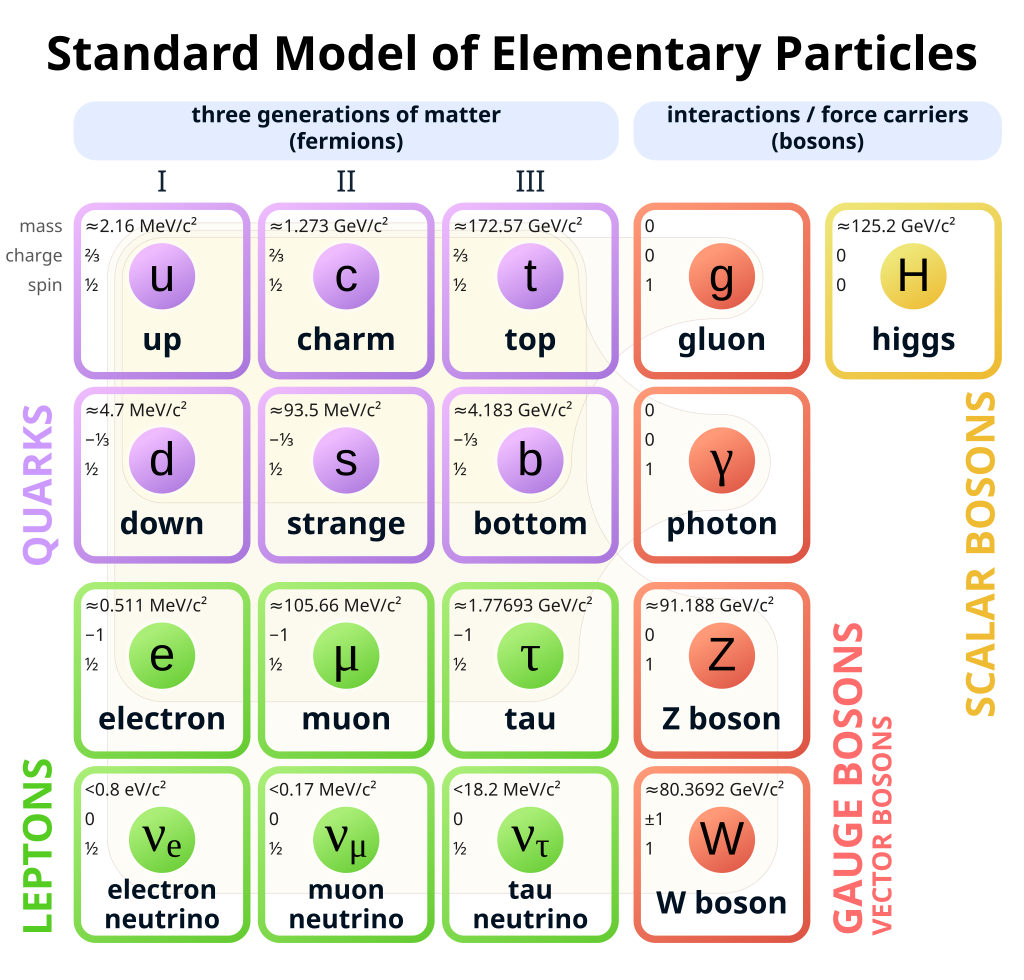
\includegraphics[width=0.75\linewidth]{media/1024px-Standard_Model_of_Elementary_Particles.svg.png}
    \caption{Standard model of elementary particles: the 12 fundamental fermions and 5 fundamental bosons \cite{cush:standard-model}.}
    \label{fig:standard_model}
\end{figure}

A key aspect of the SM is how it accounts for the masses of certain particles. While the symmetry of the SM keeps the photon massless, the W and Z bosons, which are involved in the weak force, need to have mass to match experimental observations. This happens through a process where the symmetry is hidden in the everyday world but still governs the underlying physics, known as spontaneous symmetry breaking \cite{pich2012standardmodelelectroweakinteractions}. The Higgs field, a field that fills all of space and was proposed in the 1960s by physicists like Englert, Brout, and Higgs, makes this possible. The Higgs field gives mass to the W and Z bosons and, in the process, predicts the existence of a new particle: the Higgs boson \cite{pich2012standardmodelelectroweakinteractions}.

For decades, the Higgs boson remained the missing piece of the SM. In 2012, experiments at CERN’s Large Hadron Collider (LHC), conducted by the ATLAS and CMS teams, discovered a new particle with a mass of about 125 GeV \cite{Chatrchyan_2012}. This particle’s properties have been studied extensively and align with the Higgs boson predicted by the SM, confirming the mechanism that gives mass to other particles. Today, the Higgs boson’s mass is measured to be approximately 125 GeV, with only a small uncertainty \cite{Chatrchyan_2012}.

Despite its success in explaining many experimental results, the SM is not a complete theory. It leaves several big questions unanswered. The SM does not explain why there are exactly three generations of particles, each with similar properties but different masses. It also originally assumed neutrinos had no mass, but by now it is know they have tiny masses, meaning the model needs to be adjusted.
The SM does not solve the mystery of why the Higgs boson’s mass is so small compared to what quantum effects suggest either - a problem called the hierarchy problem. These gaps suggest the SM is just part of a bigger picture that has not been fully uncovered yet. To do so, particle accelerators are used to challenge the assumptions made in the SM and even go farther - or in this case smaller and into even higher energy scales - and try to look for physics beyond the SM.

\section{The Large Hadron Collider}

To explore phenomena at distance scales far below $10^{-18}$ m (i.e. at extremely high energy scales), physicists rely on high-energy particle collisions. The LHC at CERN is the world’s largest and most powerful particle accelerator, designed to probe such distance scales by colliding protons at unprecedented energies. It is a 27 km circumference circular accelerator that accelerates two counter-rotating beams of protons to nearly the speed of light and brings them into head-on collision at four interaction points. The LHC, which design centre-of-mass energy is 14 TeV (7 TeV per beam) \cite{Evans:2008zzb}, was built to achieve a peak instantaneous luminosity of $1\times10^{34}$ cm$^{-2}$s$^{-1}$ \cite{Evans:2008zzb}. In its successful Run-1 (2010–2013) and Run-2 (2015–2018) operations, the LHC reached collision energies up to 13 TeV and even exceeded the design luminosity – achieving about $2\times10^{34}$ cm$^{-2}$s$^{-1}$ in 2018 \cite{Hayrapetyan_2024}. The machine is now in Run-3 (2022–present) with a slight energy increase (13.6 TeV). It is being upgraded for the High-Luminosity LHC (HL-LHC) era later this decade, which aims to further boost the luminosity by about an order of magnitude.

\begin{figure}[h]
    \centering
    \includegraphics[width=0.9\linewidth]{media/CCC-v2018-print-v2.pdf}
    \caption{ Sketch of the CERN accelerator complex, adapted from \cite{Mobs:2636343}.}
    \label{fig:lhc}
\end{figure}

Figure \ref{fig:lhc} shows the structure of the CERN complex with the LHC at its heart. On the discovery front, the LHC’s first triumphant success was the Higgs boson. Ongoing searches continue for signs of physics beyond the Standard Model – for example, heavy supersymmetric particles, extra dimensions, or new force carriers – across many possible decay channels. So far, no clear evidence of new particles has appeared; extensive searches in the most promising channels have found no statistically significant deviations from SM expectations \cite{sonneveld2025susyhighlightscurrentresults}.

\section{The CMS Experiment}

Collision events in the LHC produce quarks and gluons that cannot exist as free particles (colour confinement \cite{pich2012standardmodelelectroweakinteractions}). Instead, the outgoing parton radiates additional quarks and gluons, forming a parton shower whose virtuality cascades down to $\mathcal{O}(\mathrm{GeV})$, where hadronisation binds them into colour-neutral hadrons. Because soft and collinear emissions are enhanced in QCD, these hadrons emerge in a narrow cone around the original parton direction, forming a visible spray—a jet. The CMS detector is one of the two general-purpose detectors at the LHC designed to record these jets with high efficiency and precision, enabling a broad physics program from Higgs boson studies to searches for new phenomena. 

The CMS detector is built in a layered, cylindrical geometry around the collision point (see figure \ref{fig:cms_overview}) and, despite the name "Compact", enormous in absolute terms: it is about 15~m in diameter, 21~m in length, and weighs about 14,000 tonnes. At the heart of CMS is a superconducting solenoid coil that generates a magnetic field of 3.8 T within a 6~m inner diameter. This bends the trajectories of charged particles, allowing their momenta to be measured; the steel structure that contains the magnetic flux (the return yoke) also serves as the absorber for muon detection and accounts for the bulk of CMS’s mass. Inside the magnet coil, CMS is packed with high-precision tracking and calorimetry systems, and outside the coil are large muon detector chambers, as shown in figure \ref{fig:cms_overview} \cite{CMS}.

\begin{figure}[h]
\centering
    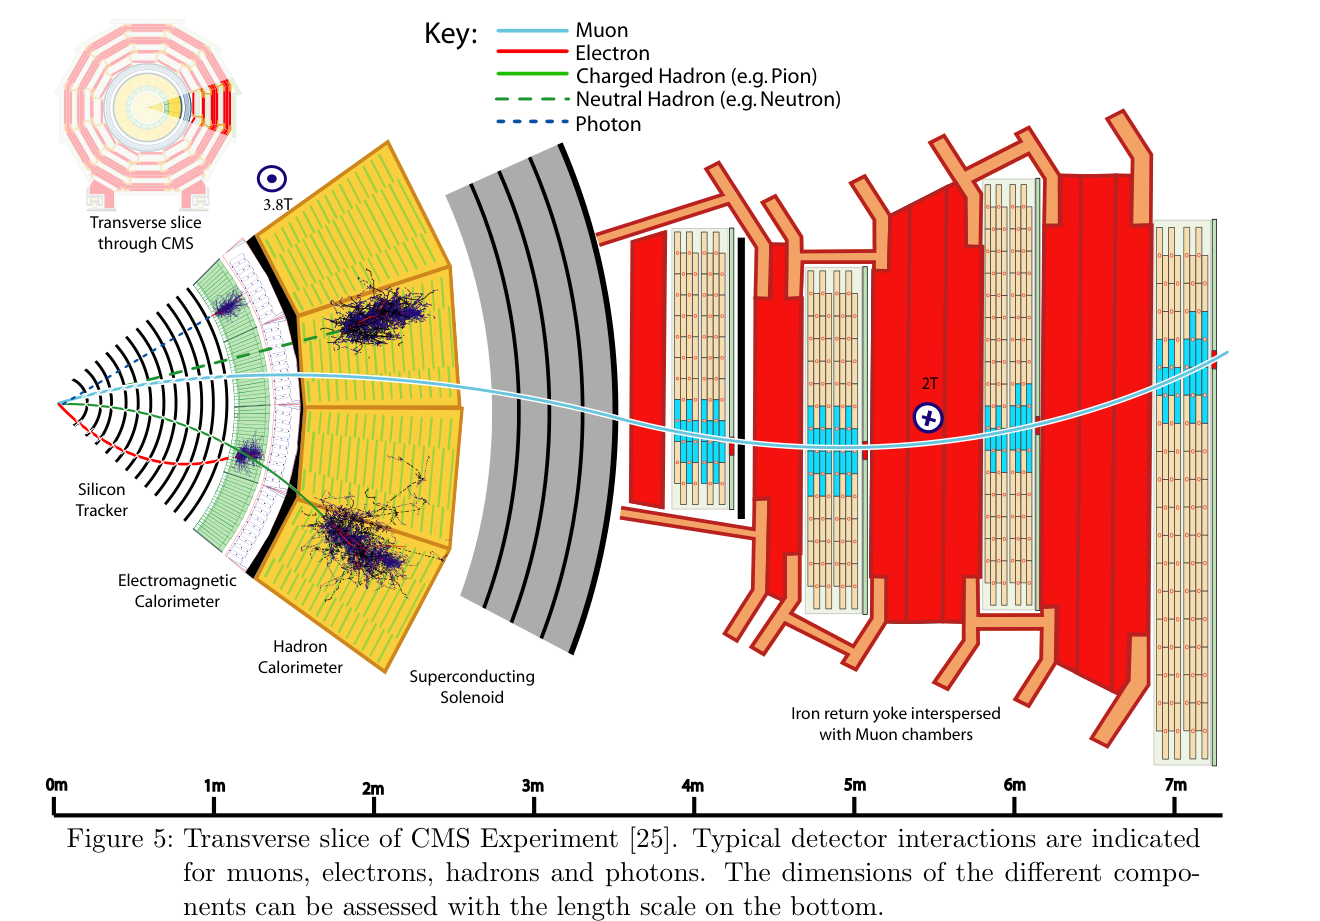
\includegraphics[width=15cm]{media/cms_cutview.png}
    \caption{Slice of the CMS Detector adapted from \cite{Sirunyan_2017}.}
    \label{fig:cms_overview}
\end{figure}

Moving outwards from the beam line, the first subsystem is the silicon tracker, a high-granularity detector made of about 75 million individual silicon strips and pixels arranged in concentric layers \cite{CMS}. When a charged particle from a collision passes through the tracker, it leaves hits in these silicon sensors. By reconstructing sequences of hits, CMS can trace out the tracks of charged particles with fine spatial resolution. The strong magnetic field bends these tracks; the particle’s momentum can be determined from the curvature. The tracker is designed to be extremely precise, allowing the reconstruction of secondary vertices from $b$-hadron decays a few centimetres from the collision point.

Surrounding the tracker is the electromagnetic calorimeter (ECAL), which is made of dense lead tungstate ($\text{PbWO}_4$) crystals. The ECAL’s task is to fully absorb and measure the energy of electrons and photons \cite{CMS}. When an electron or high-energy photon enters the ECAL, it initiates an electromagnetic shower in the crystal. The light output from the crystals is proportional to the particle’s energy. The CMS ECAL provides excellent energy resolution (on the order of 1\% for high-energy electrons/photons) and was pivotal in the Higgs boson discovery via the $H\to\gamma\gamma$ decay mode \cite{Chatrchyan_2012}.

Outside the ECAL lies the hadron calorimeter (HCAL). It is sampling calorimeter using alternating layers of absorber (brass or steel) and plastic scintillator. The HCAL is designed to stop and measure the energy of hadrons (particles made of quarks, such as pions, kaons, protons, etc.) \cite{CMS}. Hadrons penetrate the ECAL but are largely absorbed in the thicker material of the HCAL, producing cascades of secondary particles. By collecting the scintillation light from these showers, the HCAL provides a measurement of the hadronic energy. Although the HCAL’s resolution is coarser than that of the ECAL, combining its information with the ECAL and tracker allows reconstruction of the energy and direction of jets as well as the estimation of missing transverse energy.

The outermost layers of CMS are the dedicated muon detectors, which give the experiment its name. Muons are charged leptons similar to electrons but about 200 times heavier, and they are penetrating: unlike most particles, muons can traverse substantial amounts of matter. In CMS, after passing through the calorimeters, muons still have enough energy to reach the muon chambers interleaved in the steel return yoke \cite{CMS}. CMS employs several types of muon detectors (drift tubes, cathode strip chambers, and resistive plate chambers) to track muons independently of the inner tracker. By matching muon tracks in the muon system with those in the inner tracker, CMS achieves a very accurate muon momentum measurement.

\subsection{Trigger System}
As the LHC collision rate is enormous, CMS cannot record data from every collision. Instead, the experiment uses a trigger system to filter events in real time. CMS employs a two-level trigger system: a Level-1 (L1) trigger implemented in custom electronics (fast hardware logic) and a High-Level Trigger (HLT) implemented in software running on a computing farm \cite{Khachatryan_2017}. The L1 trigger, which is using information from the calorimeters and muon system, reduces the 40 MHz collision rate to around 100 kHz by selecting events with interesting signatures (such as high-energy objects). Then the HLT takes those L1-selected events and runs a streamlined version of the full event reconstruction to apply more refined selection criteria, outputting a final rate of around 1 kHz to permanent storage \cite{Khachatryan_2017}. This multi-tiered trigger is crucial for ensuring that the most interesting collisions – those potentially containing rare new physics or useful signals – are recorded for offline analysis, while discarding the rest.

\subsection{Coordinates}
CMS uses a right-handed coordinate system with the origin at the centre of the detector. The x-axis points radially inward toward the centre of the LHC ring, the y-axis points vertically upward, and the z-axis is aligned with the beam direction (pointing towards the Jura mountains) \cite{Chatrychan_2008}. Instead of simple Cartesian coordinates $(x,y,z)$, it is often convenient to use cylindrical and spherical coordinates $(r,\phi,\theta)$ (or equivalently $(r,\phi,\eta)$) to describe angles and distances. Here, $r$ denotes the distance from the beam line in the transverse plane ($x$–$y$ plane), $\phi$ is the azimuthal angle in that plane (with $\phi=0$ defined along the positive x-axis), and $\theta$ is the polar angle measured from the positive $z$-axis.

In practice, the polar angle $\theta$ is expressed via the pseudorapidity $\eta$, defined as:

\begin{equation}
    \eta = - \ln \left( \tan \frac{\theta}{2}\right)
\end{equation}

For highly relativistic particles (with $E \gg m$), the pseudorapidity $\eta$ is approximately equal to the particle’s rapidity $y$, which is given by

\begin{equation}
    y = \frac{1}{2} \ln\frac{E+p_z}{E-p_z},
\end{equation}

where $E$ is the particle’s energy and $p_z$ is the $z$-component of the momentum; the transverse momentum is $p_T=\sqrt{p_x^2+p_y^2}$. This coordinate choice conveniently captures the detector’s cylindrical symmetry and the boost-invariant nature of motion along the beam axis \cite{Chatrychan_2008}.

% Chapter 2
\chapter{Machine Learning in High Energy Physics (HEP)}

Machine-learning (ML) methods play an increasingly central role in high-energy-physics analyses, from low-level detector reconstruction to high-level statistical inference \cite{PhysRevD.112.016004}. Their usefulness derives from the ability to learn complex, non-linear correlations in high-dimensional feature spaces that are difficult to express in analytic form. Historically, particle physicists pioneered the use of multivariate algorithms in the 1990s and 2000s for analysis tasks, relying on techniques like artificial neural networks and boosted decision trees (BDTs) \cite{Guest_2018}. The emergence of deep learning around 2012 enabled training of very large neural networks that outperformed previous state of the art models \cite{Guest_2018}. This caused a rapid expansion of HEP applications spanning across particle/event identification, reconstruction and even real-time data filtering \cite{albertsson2019machinelearninghighenergy}.


\section{Machine Learning using Deep Neural Networks}

Neural networks (NNs) are computational models designed to approximate a mapping from input variables \textbf{x} to a desired output \textbf{y}. They consist of interconnected nodes organized into layers, inspired by the structure of the human brain \cite{hammad2024artificialneuralnetworkdeep}. The input layer contains one node for each dimension of the training data. The output layer corresponds to the desired output dimensions, reflecting the number of distinct mappings the network needs to learn. Between input and output layer, a varying number of hidden layers number enhance the network’s ability to adapt and model complex patterns. Each node is associated with a weight, a bias, and an activation function, enabling non-linear mappings for intricate problems \cite{Goodfellow-et-al-2016}. During training, a process called backpropagation adjusts these weights by computing gradients across the network from input to output, guided by a specified loss function.

When the number of hidden layers increases significantly, the network is typically referred to as a deep neural network (DNN), capable of modelling highly complex relationships in data. DNNs can approximate arbitrarily complicated functions, making them well-suited for tasks such as particle identification, energy regression, pile-up mitigation, and anomaly detection \cite{Khalaf:2025grv}. In practice, DNN-based algorithms now permeate the workflow of collider and astroparticle experiments, achieving better performance than many traditional methods. For example, convolutional neural networks (CNNs) that treat detector data as images have outperformed physics-motivated features in classifying jet substructure \cite{de_Oliveira_2016}. Likewise, recurrent neural networks (RNNs) or long short-term memory (LSTM) networks can naturally handle sequential data, as demonstrated by their use in jet flavour taggers to process tracks and vertex sequences \cite{Bols_2020}.

A typical supervised-learning workflow in HEP involves several common steps. First, labelled datasets are prepared using Monte Carlo (MC) simulations, which provide ground-truth information for particle types, kinematics, event categories, etc. Supervised training on MC truth is widespread because real collisions cannot be labelled event-by-event with the desired signal/background distinctions \cite{PhysRevD.112.016004}. However, ML models can overfit to simulation-specific artifacts, potentially limiting their ability to generalize to real data \cite{PhysRevD.112.016004}. To mitigate this, physicists carefully design training procedures and validation tests. The dataset is typically split into training and testing portions; models are trained with a suitable loss function (for example, cross-entropy for classification or mean squared error for regression) which reflects the physics goals. Sometimes custom objectives are used – for instance, optimizing directly for a statistical significance metric or incorporating systematic uncertainty penalties – but this is balanced against practical considerations (differentiability, training stability) \cite{Bardhan:2024ibw}.

\section{Adversarial Machine Learning}

Adversarial machine learning studies how deliberately crafted inputs — or unintentional mismodelling — can cause an ML model to make incorrect or biased predictions \cite{doi:10.1142/12294}. In computer vision, the addition of nearly imperceptible perturbations to an image can fool a deep classifier into misidentifying objects \cite{Stein2022}. Resistance to small perturbations is also important in HEP context: Recent studies have raised awareness that supervised HEP models may latch onto simulator-specific quirks — for example, subtle differences in detector response modelling — such that they fail to generalize to real data \cite{PhysRevD.112.016004}. These quirks make HEP models susceptible to data-simulation discrepancies: a slight miscalibration in the simulation or a tiny adjustment in the input features might cause disproportionate shifts in the model output. Ensuring robustness against these effects is therefore important, especially as ML algorithms are integrated into critical physics results.  

\subsection{Adversarial Attacks}

Most textbook adversarial attacks assume continuous, differentiable input spaces (such as pixel intensities in an image) and rely on gradient information to find an effective perturbation. For instance, the Fast Gradient Sign Method (FGSM) and the Projected Gradient Descent (PGD) (see Chapter 4 for detailed descriptions) are two well-known techniques that use the gradient of the model’s loss with respect to the input features to adversarially tweak the input \cite{goodfellow2015explainingharnessingadversarialexamples}. These methods nudge the input in the direction that most increases the model’s error, subject to a constraint on the perturbation size (often measured by an $L_p$ norm). FGSM accomplishes this in one step using the sign of the gradients, while PGD applies multiple small steps iteratively and projects the result to ensure the perturbation is staying within a norm bound \cite{madry2019deeplearningmodelsresistant}. Other attack methods include DeepFool, which finds the smallest perturbation to cross the decision-boundary, and various black-box attacks that do not require gradient access. These techniques have been successfully applied in computer vision, where inputs are continuous pixel arrays and small changes can be carefully crafted to cause misclassifications.

Applying adversarial attacks in HEP is challenging due to the constrained realm of physical features. Despite those complications, researchers have begun to explore HEP-specific adversarial attacks. Initial studies have shown that HEP classifiers are susceptible to small input distortions on continuous input features; one group systematically applied FGSM perturbations to a jet-tagging network's input and found that the classifier's performance degraded significantly \cite{Stein2022}. This is not surprising, given that many networks used in HEP rely on piecewise linear activation functions and high-dimensional feature spaces. Consequently, perturbation of a single high-level feature — analogous to the "one-pixel-attack" in images — could potentially flip a classification if the network is right at a decision boundary \cite{Stein2022}.

\subsection{Adversarial training}

Adversarial training is a defence technique wherein the model is trained on deliberately perturbed examples in addition to the nominal data. In practice, this means augmenting each training batch with adversarial modified inputs and using them with the correct labels to update model parameters (see Figure \ref{fig:adversarial_training}). By learning from these fraudulent examples, the model's decision boundaries become smoother and less sensitive to tiny fluctuations in input features \cite{goodfellow2015explainingharnessingadversarialexamples}.

\begin{figure}
    \centering
    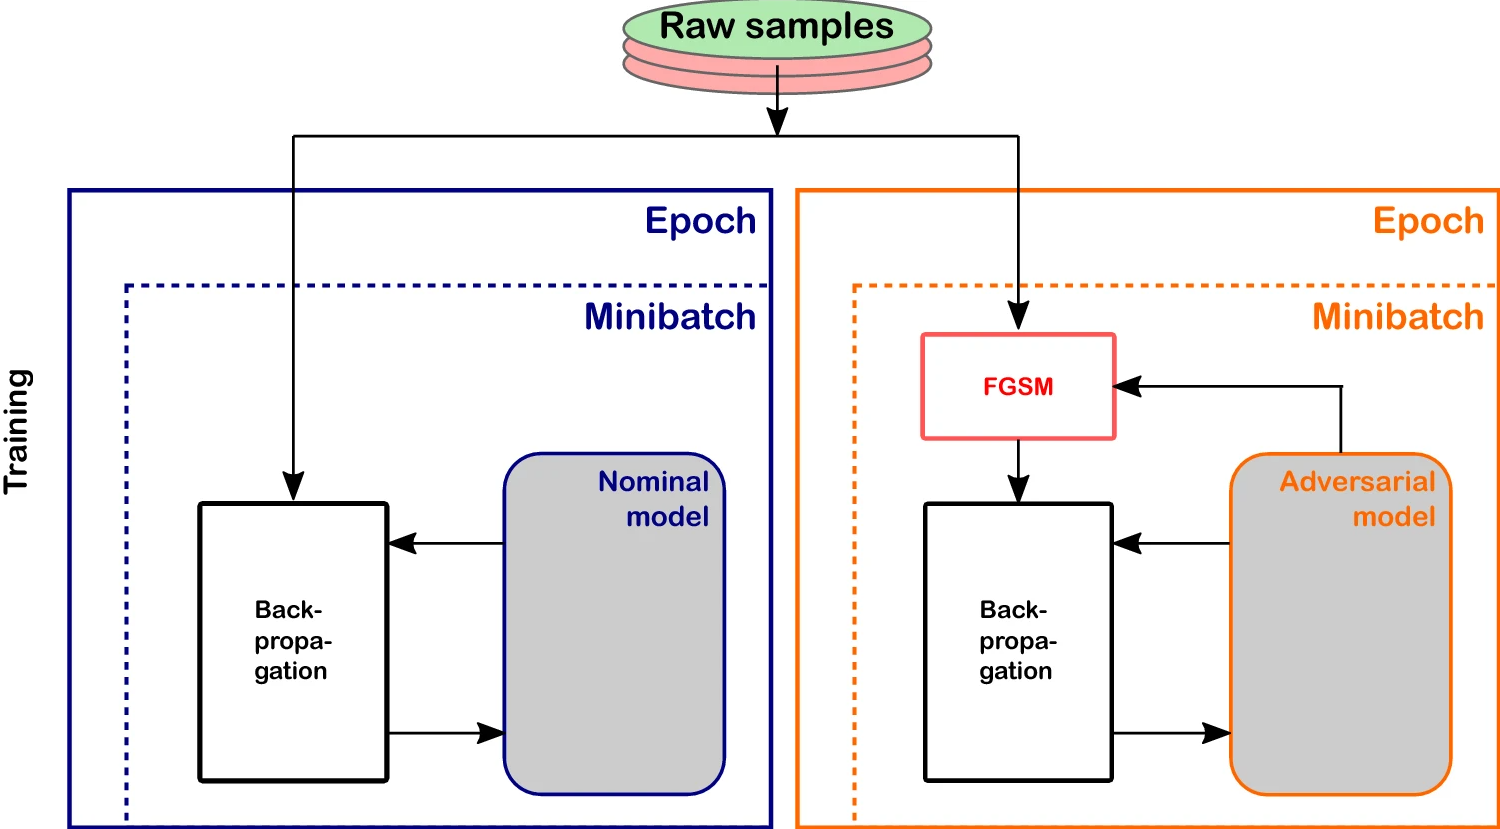
\includegraphics[width=0.8\linewidth]{media/adversarial_training.png}
    \caption{Comparison between nominal and adversarial training procedure for a neural network. The network on the right is trained on adversarial samples that are designed to fool the network, generated by the PGD attack. By training on the adversarial examples, the network is less susceptible to adversarial attacks \cite{Stein2022}.}
    \label{fig:adversarial_training}
\end{figure}

In HEP, adversarial training reduces reliance on simulator-specific quirks and improves resilience to mismodelling. For example, if a tagger leans on a mismodelled feature, training with amplified versions of that mismatch pushes the network to learn more robust discriminants. This strategy was demonstrated by injecting slight perturbations into jet features during training — effectively simulating systematic shifts — and showed that the resulting tagger maintained high nominal performance while becoming significantly less vulnerable to such shifts \cite{Stein2022}. The adversarially-trained model coped better with variations in detector response and particle distribution, suggesting improved generalization to real data.

\section{The DeepJet Tagger}
\label{sec:DeepJet}

The DeepJet tagger represents a successful application of deep learning to a classic HEP problem by distinguishing heavy-flavour jets from light-quark or gluon jets. These taggers employ hierarchical neural-network architectures to combine information from many low-level inputs and produce a single probability for each flavour category. The key insight of DeepJet is to use as much information as possible about each jet, instead of relying on a hand-selected subset of inputs as previous algorithms did \cite{Bols_2020}. Earlier-generation taggers like CSV/DeepCSV used a fixed number of high-quality tracks and secondary vertices as input. In contrast, DeepJet forgoes a broad preselection of jet constituents; it ingests an extensive list of per-particle features – including charged and neutral particle-flow candidates, secondary vertex properties, and global jet attributes – and makes the neural network learn which features are important \cite{Bols_2020}.

\subsection{Candidate selection}

The candidate preselection is built on jets reconstructed using the particle-flow (PF) algorithm of CMS. Jets are clustered from PF candidates with the anti-$k_T$ algorithm that is based on the distance between constituents of the jet \cite{Tumasyan_2022}. The PF event reconstruction identifies and reconstructs individual particles (photons, electrons, muons, charged/neutral hadrons) by optimally combining information from all subdetectors \cite{Tumasyan_2022}. This provides a detailed list of charged and neutral particle candidates for each jet, along with any reconstructed secondary vertices from decays of long-lived particles.

All PF candidates associated with a jet – both charged and neutral – are used as inputs, supplemented by up to four secondary vertices and a set of global jet features. To maintain a fixed-size input representation, a maximum of 25 charged PF candidates and 25 neutral PF candidates are included per jet. This “no strict preselection” approach retains as much information as possible, avoiding the loss of potentially useful tracks that earlier methods discarded \cite{Bols_2020}.

\subsection{Architecture}

\begin{figure}[h]
    \centering
    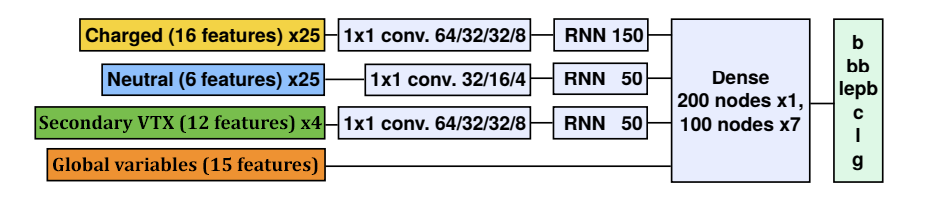
\includegraphics[width=1\linewidth]{media/deepJet_architecture.png}
    \caption{Illustration of the DeepJet architecture, adapted from \cite{Bols_2020} to fit our dataset (see \ref{sec:dataset}). Charged and neutral particle-flow
candidates, secondary vertices, and global variables are used as inputs to the tagger, which are processed by the hidden layers (white). The model outputs the probabilities for a jet to belong to one of the six jet classes.}
    \label{fig:deepjetArchitecture}
\end{figure}

The DeepJet Tagger takes 15 global input variables, 16 charged ParticleFlow (CPF) input variables for 25 candidates, 6 neutral ParticleFlow (NPF) input variables for 25 candidates and 12 secondary vertex (SV) input variables for 4 candidates, constituting 613 inputs per jet (see figure \ref{fig:deepjetArchitecture}). In the first stage, separate input streams are established for each type of low-level object: one for charged particles (tracks), one for neutral particles, and one for secondary vertices. Each stream passes through a stack of $1\times1$ convolutional layers with \textit{kernel size = 1} with bias parameters. These layers compute per-particle features without mixing information across particles, so each particle receives the same operation regardless of order \cite{Bols_2020}. Essentially, this track learns a representation for each track, each neutral, and each vertex input. Next, the outputs of these convolutional streams are fed into recurrent layers (LSTMs \cite{Goodfellow-et-al-2016}). The charged candidate LSTM uses 150 nodes, the neutral LSTM and secondary vertex LSTM each use 50 nodes. The LSTM outputs then are fed into a dense layer of 200 nodes followed by seven layers of 100 nodes each, using ReLU activation throughout. The final output layer is based on a softmax activation function and consists of six nodes, which are the model outputs for the six jet categories.

% Chapter 3
\chapter{Methodology}

\section{Initial Epxloration of PDG}
Lorem ipsum set dolor.

\subsection{PGD on Continious Inputs}
Lorem ipsum set dolor.

\subsection{PGD with naive Integer Handling}
Lorem ipsum set dolor.

\section{Probabilistic Integer Pertubation (IntProb)}
Lorem ipsum set dolor.

\section{Combination of PGD and IntProb}
Lorem ipsum set dolor.

\section{Implementation Details}
Lorem ipsum set dolor.

\subsection{Feature Relevance and Input Clamping}
Lorem ipsum set dolor.

\subsection{Integration into DeepJet Framework}
Lorem ipsum set dolor.

\section{Evaluation Metrics and Threat Model}
Lorem ipsum set dolor.


% Chapter 4
\chapter{Adversarial Studies on DeepJet}

To evaluate the performance of adversarial attacks, the models nominal performance is assessed as a baseline for unperturbed input data. Based on this data, the input similarity (see \ref{sec:input_similarity}) is addressed for multi-iterational attacks of PGD, PIP and PIP-PGD. Furthermore, a PGD attack is applied as a reference for a successful attack. The JSD value is used throughout this entire chapter to quantify the mismatching of the given adversarial input. ROC Curves act as labels for the success of the attacks while being complemented by additional loss/validation curves that offer a broader view of the attacks performance. All attacks are evaluated in terms of attack severity, performance on nominal data, and adversarial-trained performance, followed by an analysis of their transferability and cross-robustness to determine whether PIP — alone or in combination with continuous-domain attacks — offers robustness beyond existing methods.

\section{Reference study}

This section establishes critical benchmarks for evaluating adversarial attacks on DeepJet. It first assesses the model's nominal performance under standard conditions to provide a baseline for unperturbed data. Then, it examines the impact of PGD attacks to set a reference for comparing subsequent adversarial strategies.

\subsection{Nominal Performance}

At nominal training and testing, the training validation yields a stable curve with a convergence at around 0.93. The validation is sitting slightly below at roughly 0.90 offering stable convergence too (see figure \ref{fig:nominal_training}). Figure \ref{fig:nominal_roc} portrays the identification score for BvsL found to be $AUC=0.965$.

\begin{figure}[htbp]
  \centering
  \begin{subfigure}[t]{0.59\textwidth}
    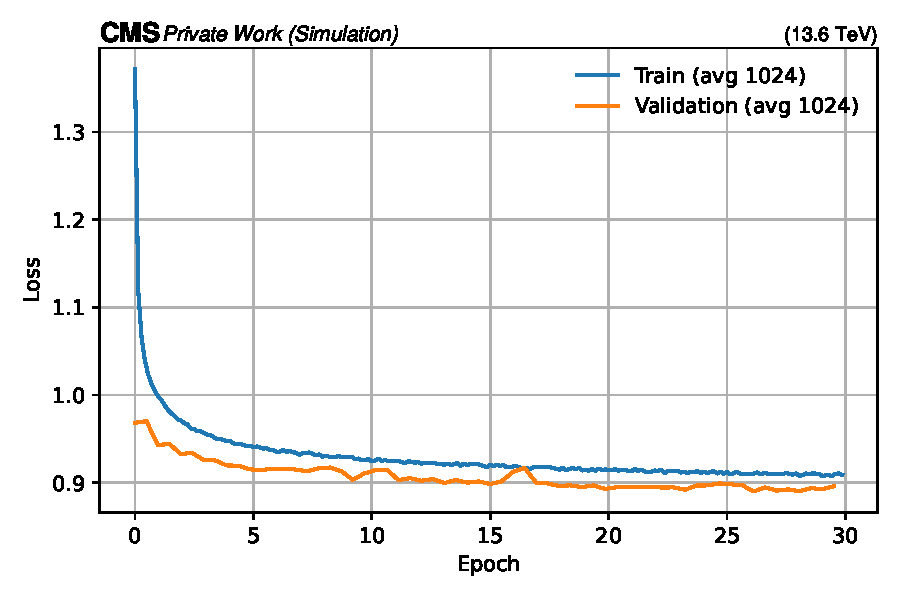
\includegraphics[width=\linewidth]{media/output/nominal_loss_validation.pdf}
    \caption{Training and validation loss for nominal training up to 30 epochs.}
    \label{fig:nominal_training}
  \end{subfigure}\hfill
  \begin{subfigure}[t]{0.41\textwidth}
    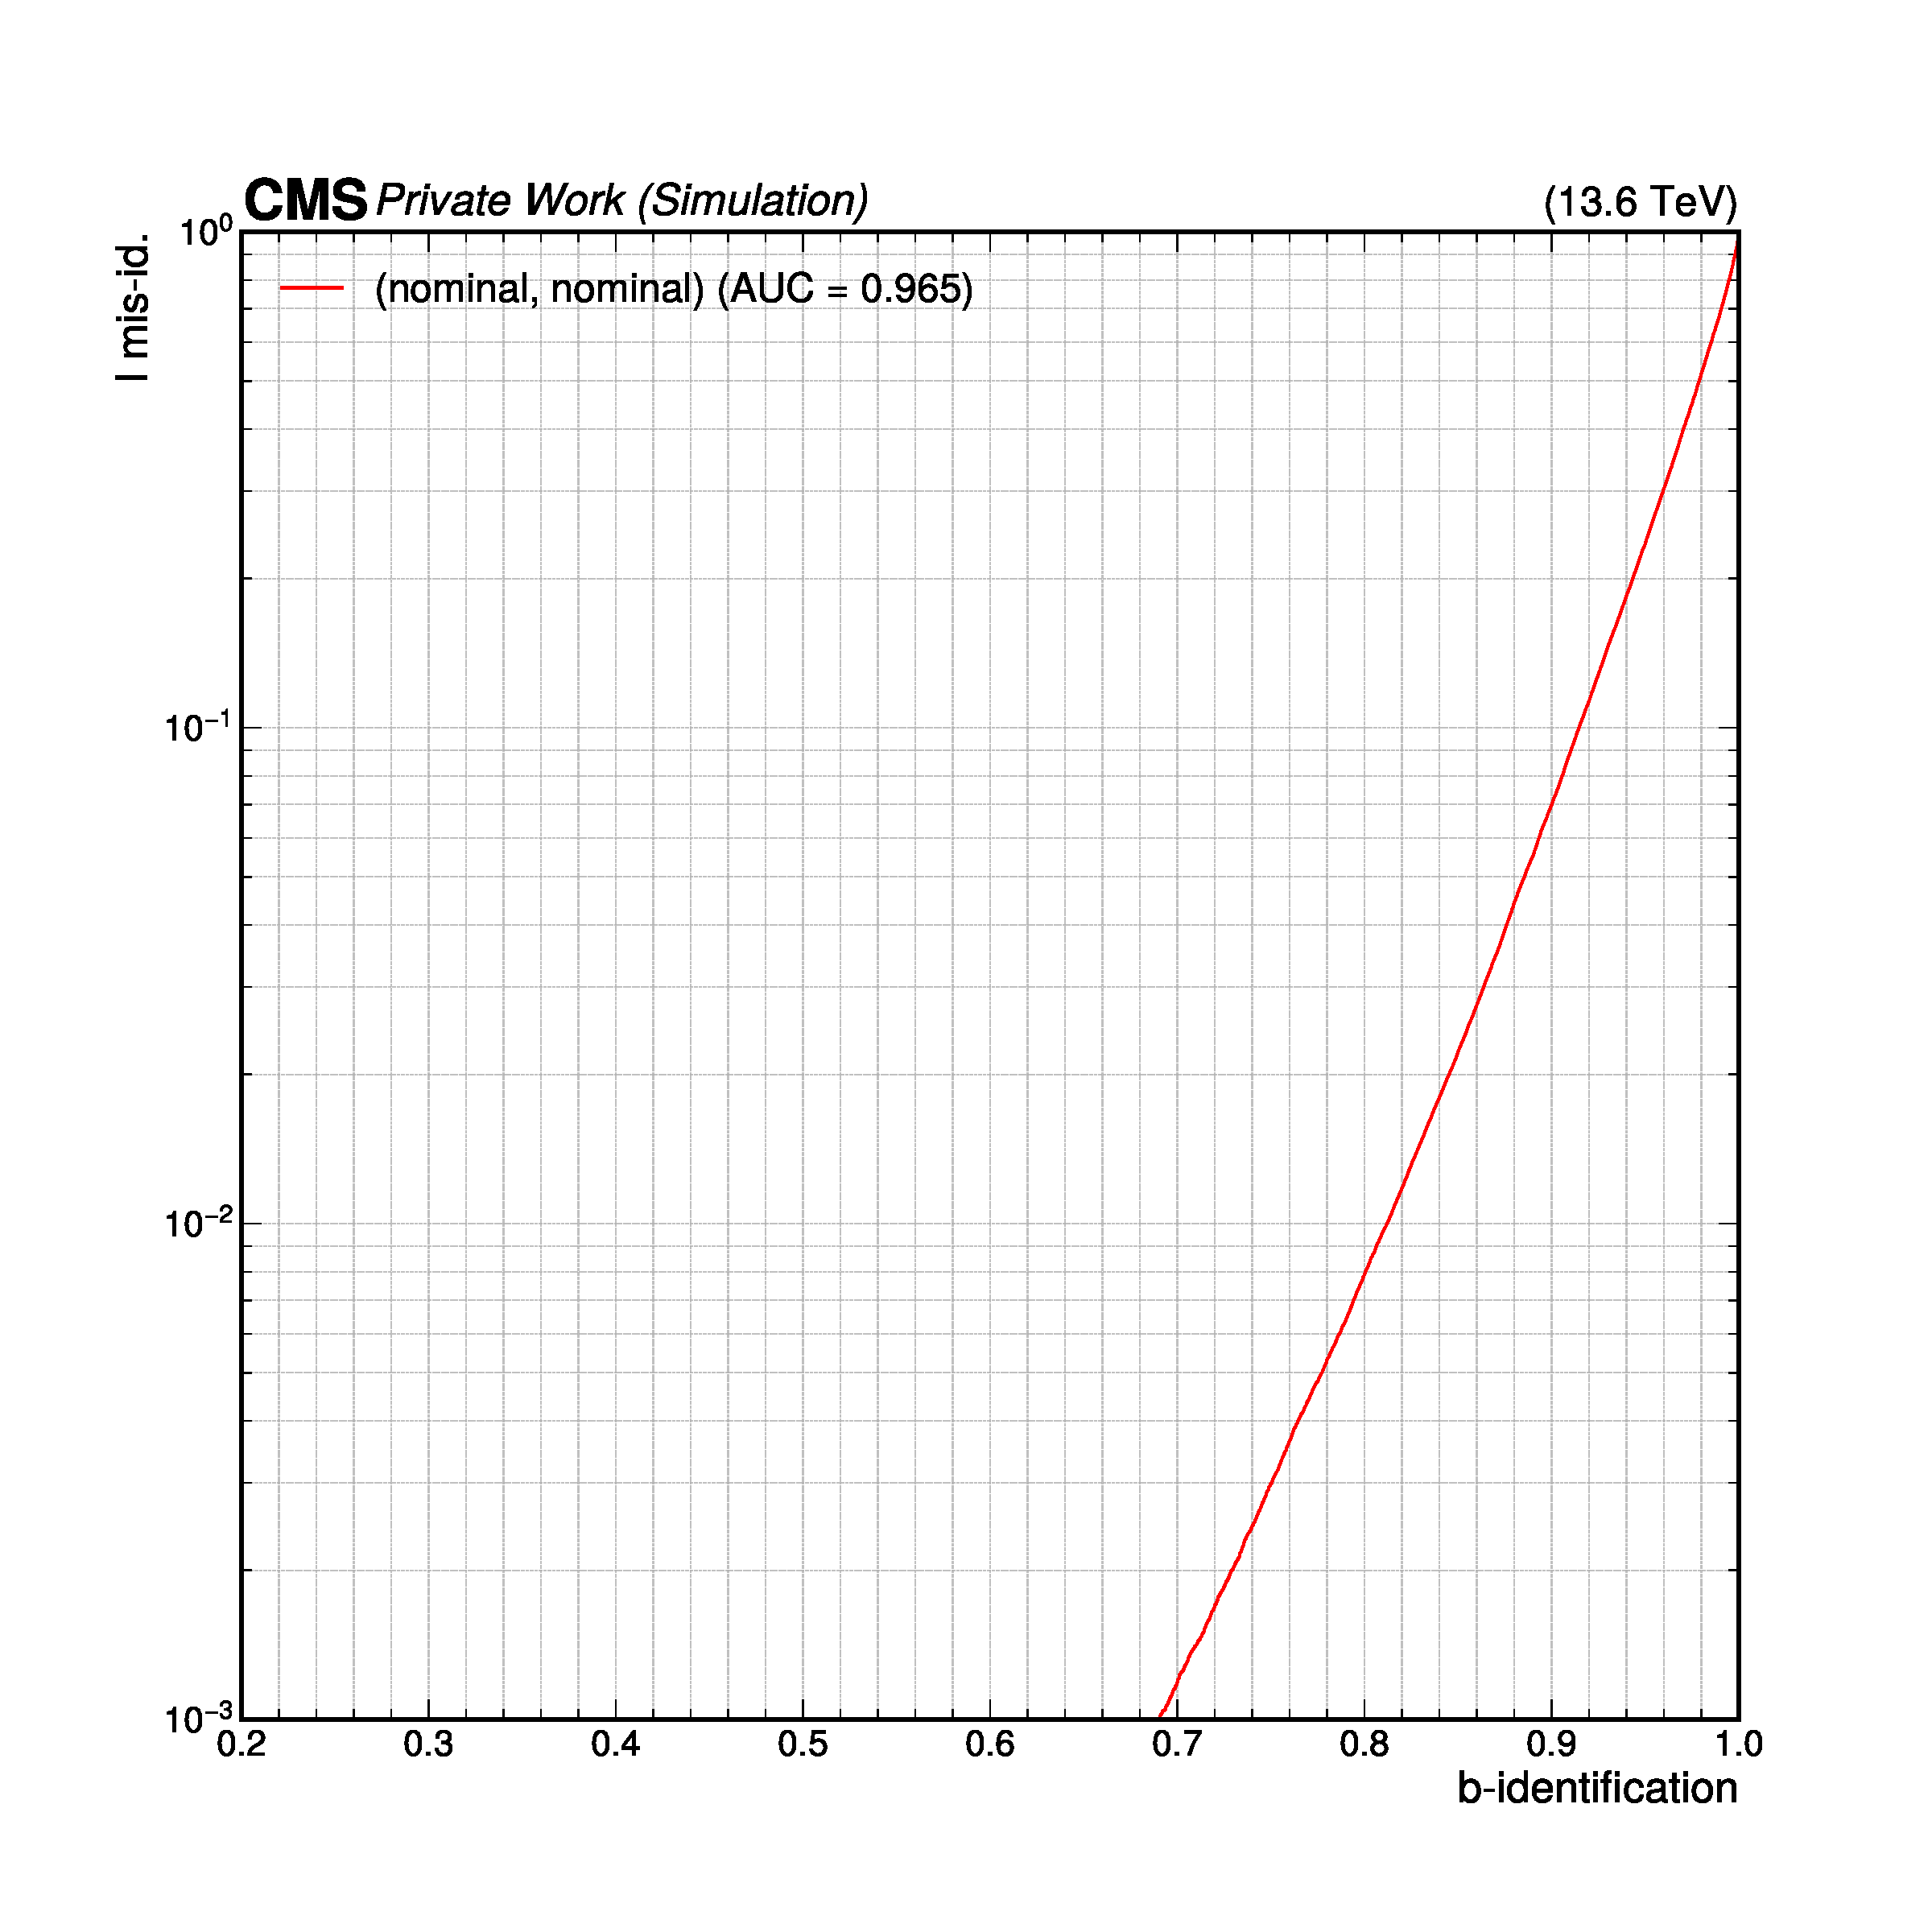
\includegraphics[width=\linewidth]{media/output/roc_bvsl_nominal_nominal.pdf}
    \caption{ROC Curve for the nominal trained baseline tested against nominal input.}
    \label{fig:nominal_roc}
  \end{subfigure}\hfill
\end{figure}

\FloatBarrier
\subsection{Projected Gradient Descent}

To assess the efficacy of the novel approach it is also necessary to look at well established adversarial attacks as an adversarial baseline — in this case PGD. For the sake of simplicity a magnitude of $\epsilon=0.1$ is applied for all following PGD attacks\footnote{As briefly discussed in section \ref{sec:fgsm_methodology} an additional scaling is applied proportional to the relative feature scale tensor $\varepsilon_{i,i}$. The behaviour for varying PGD magnitudes does not fall into the scope of this thesis.}.

\paragraph{Severity:} Figure \ref{fig:pgd_input_overview} provides a comprehensive view of input similarity across the entire input domain for up to three PGD iterations. The figure reveals an important patterns: 
(1) The JSD values for all features and iterations fall within the range of $\mathcal{O}(10^{-2})$ to $\mathcal{O}(10^{-3})$, in agreement to the threshold typically considered for stealthy attacks.
(2) The perturbation magnitude generally stays constant over multiple iteration. However, this is not uniform across all features; some features show minimal change even after multiple iterations, while others exhibit significant perturbation from the first iteration.

This selective perturbation behaviour stems from the gradient reassessment process inherent in PGD. Unlike single-step methods like FGSM that always assume the worst-case perturbation direction, PGD's iterative approach allows for more nuanced optimization. Features with strong gradients in the initial iterations may see their gradients diminish or even reverse direction in subsequent iterations, causing them to "project back" toward their original values. The overall perturbation pattern suggests that PGD attacks are highly targeted. They focus computational effort on features that provide the most leverage for compromising the classifier's performance.

\begin{figure}[H]
\centering
    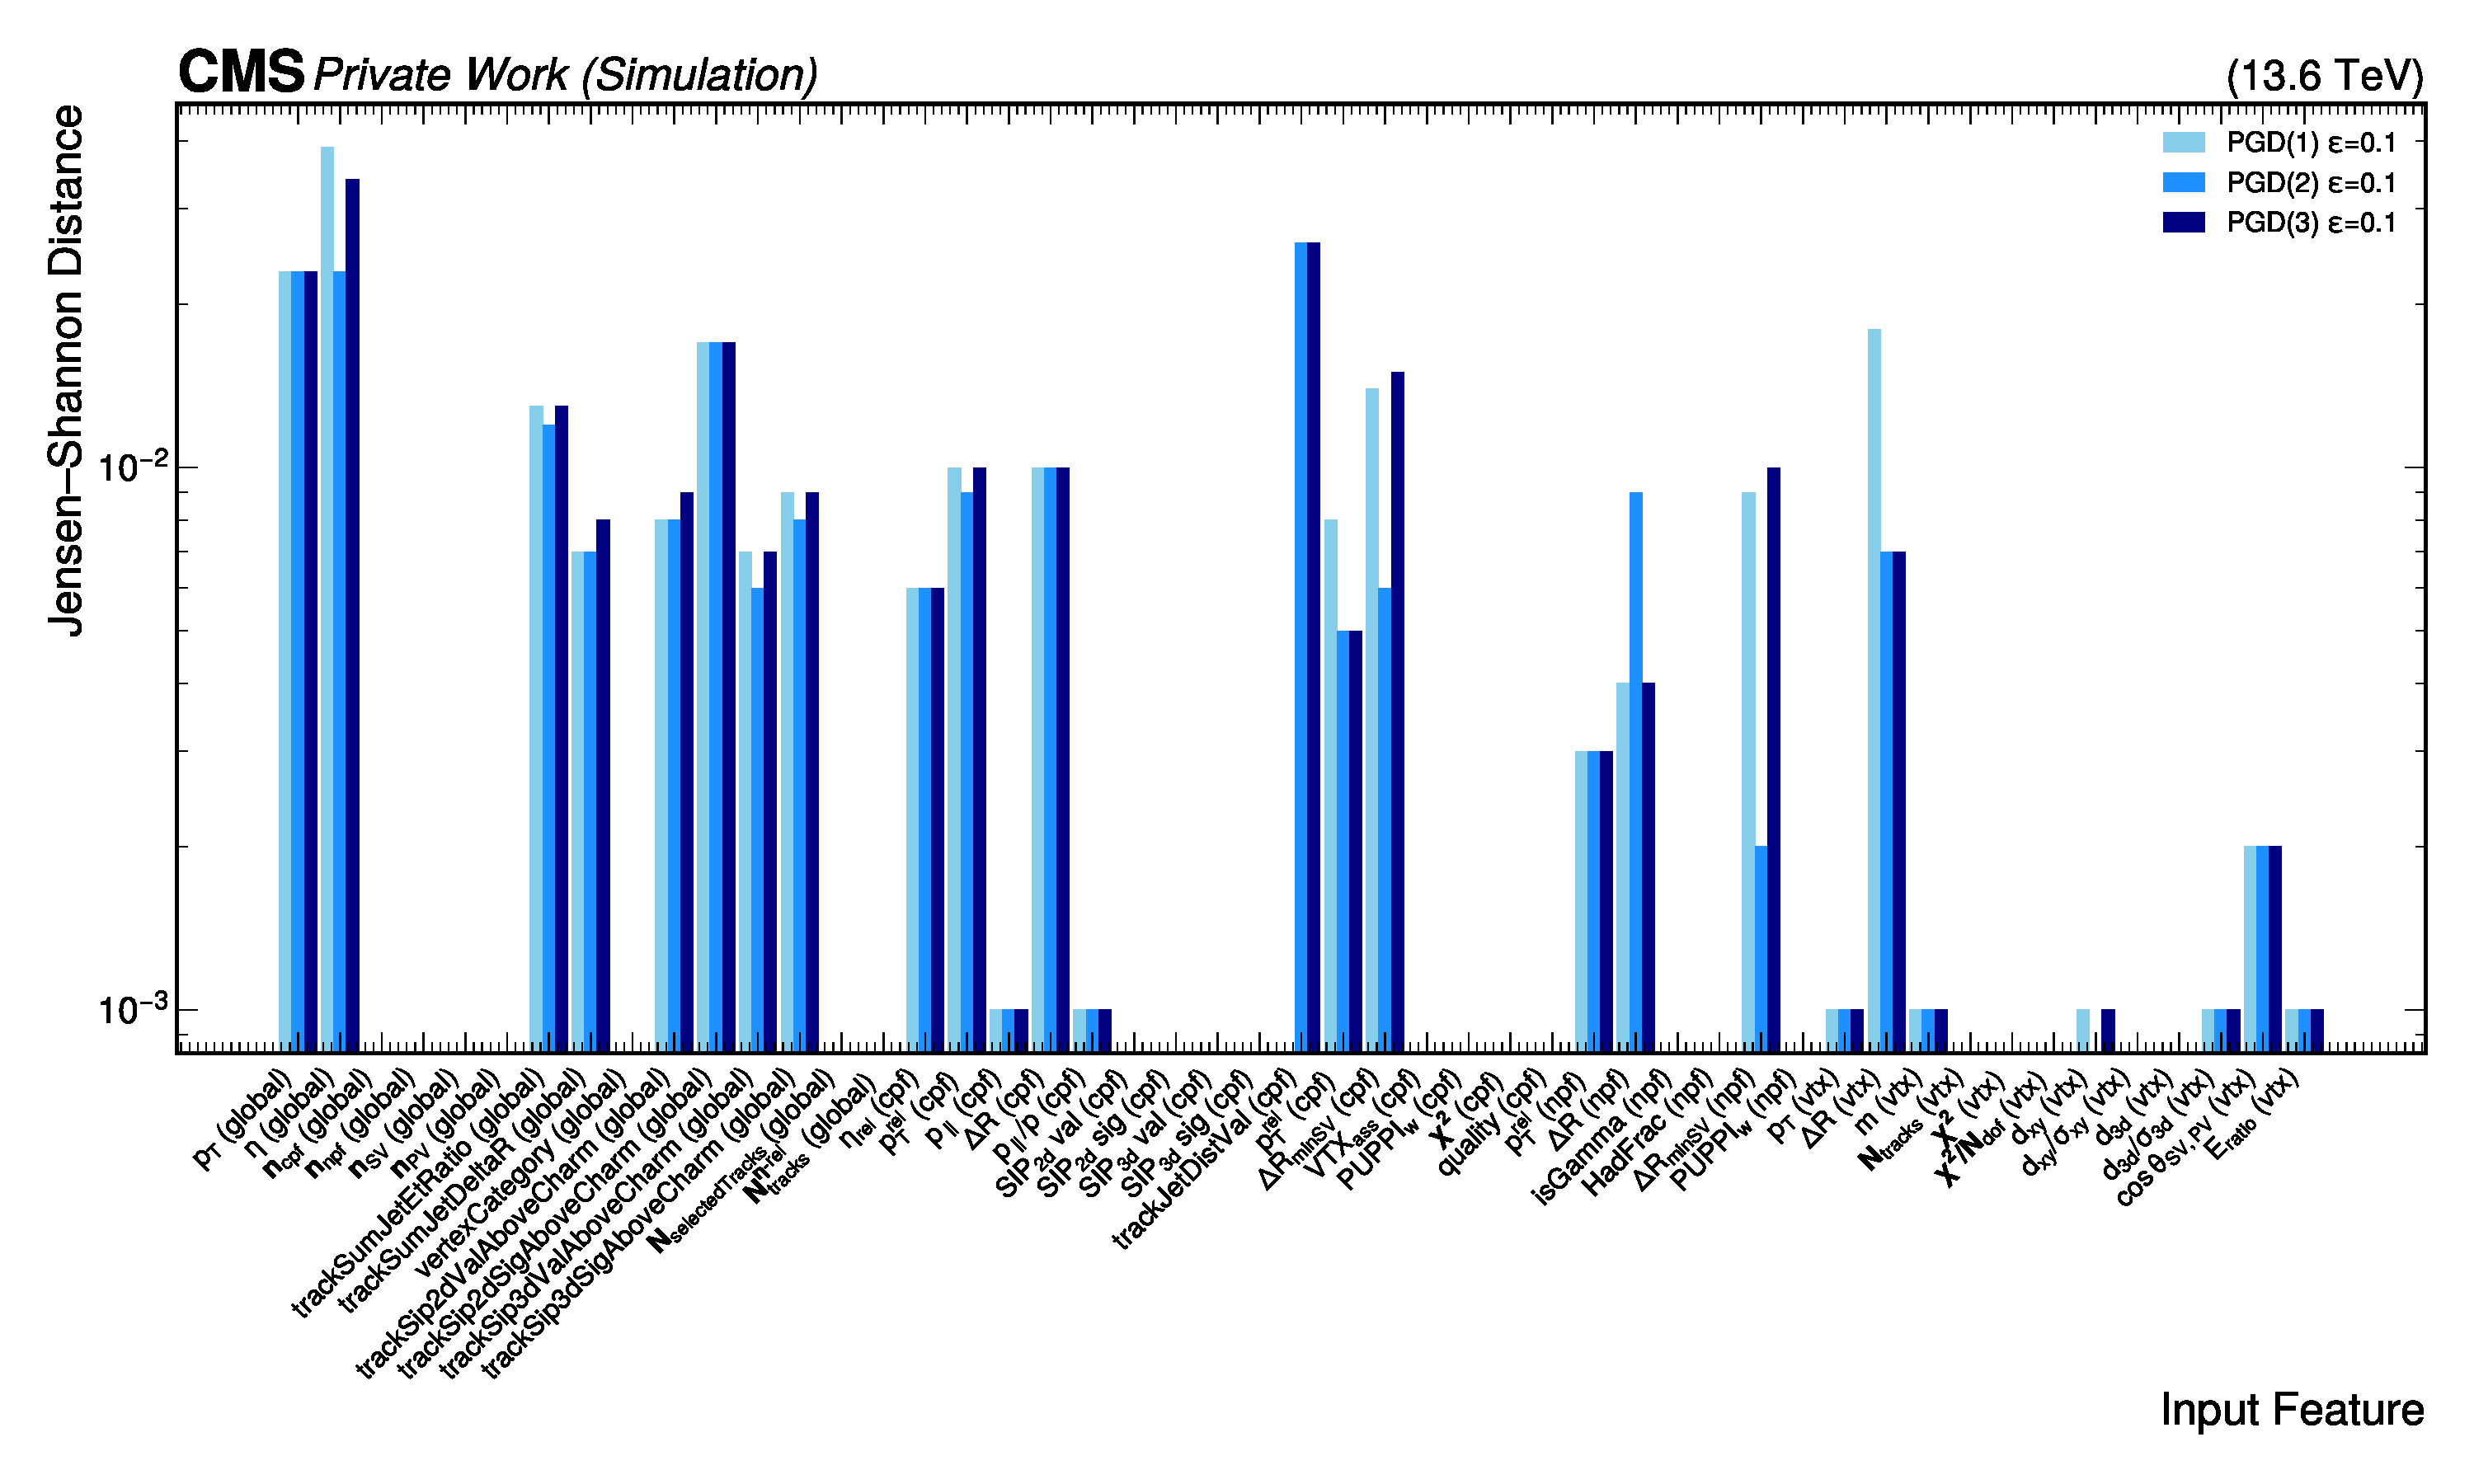
\includegraphics[width=15cm]{media/output/features/compare/jsd_pgd_iterations_featurewise_hor.pdf}
    \caption{JSD input similarity development for up to three iterations of the PGD attack with $\epsilon=0.1$ tested against a nominal trained model.}
    \label{fig:pgd_input_overview}
\end{figure}
\FloatBarrier
\newpage
\paragraph{Attack:} Figure \ref{fig:pgd_iterations} illustrates the impact of multiple PGD iterations on the BvsL discrimination task. The baseline nominal performance (AUC = 0.965) serves as the reference point against which attack efficacy is measured. The single-iteration PGD(1) attack achieves an AUC of approximately $0.937$, representing a clear reduction in performance. This initial attack demonstrates that even minimal adversarial perturbation can compromise the classifier's discriminative power. The two-iteration PGD(2) attack yields the same AUC score as PGD(1), while the three-iteration variant  reduces the AUC slightly to approximately 0.936.

This progressive degradation highlights two important aspects of PGD attacks. The iterative nature allows for more sophisticated perturbation strategies that can exploit the model's decision boundaries more effectively than single-step methods. Moreover, the diminishing returns observed between iterations 2 and 3 suggest that the attack approaches a performance floor, beyond which additional iterations provide minimal benefit.

\begin{figure}[h]
\centering
    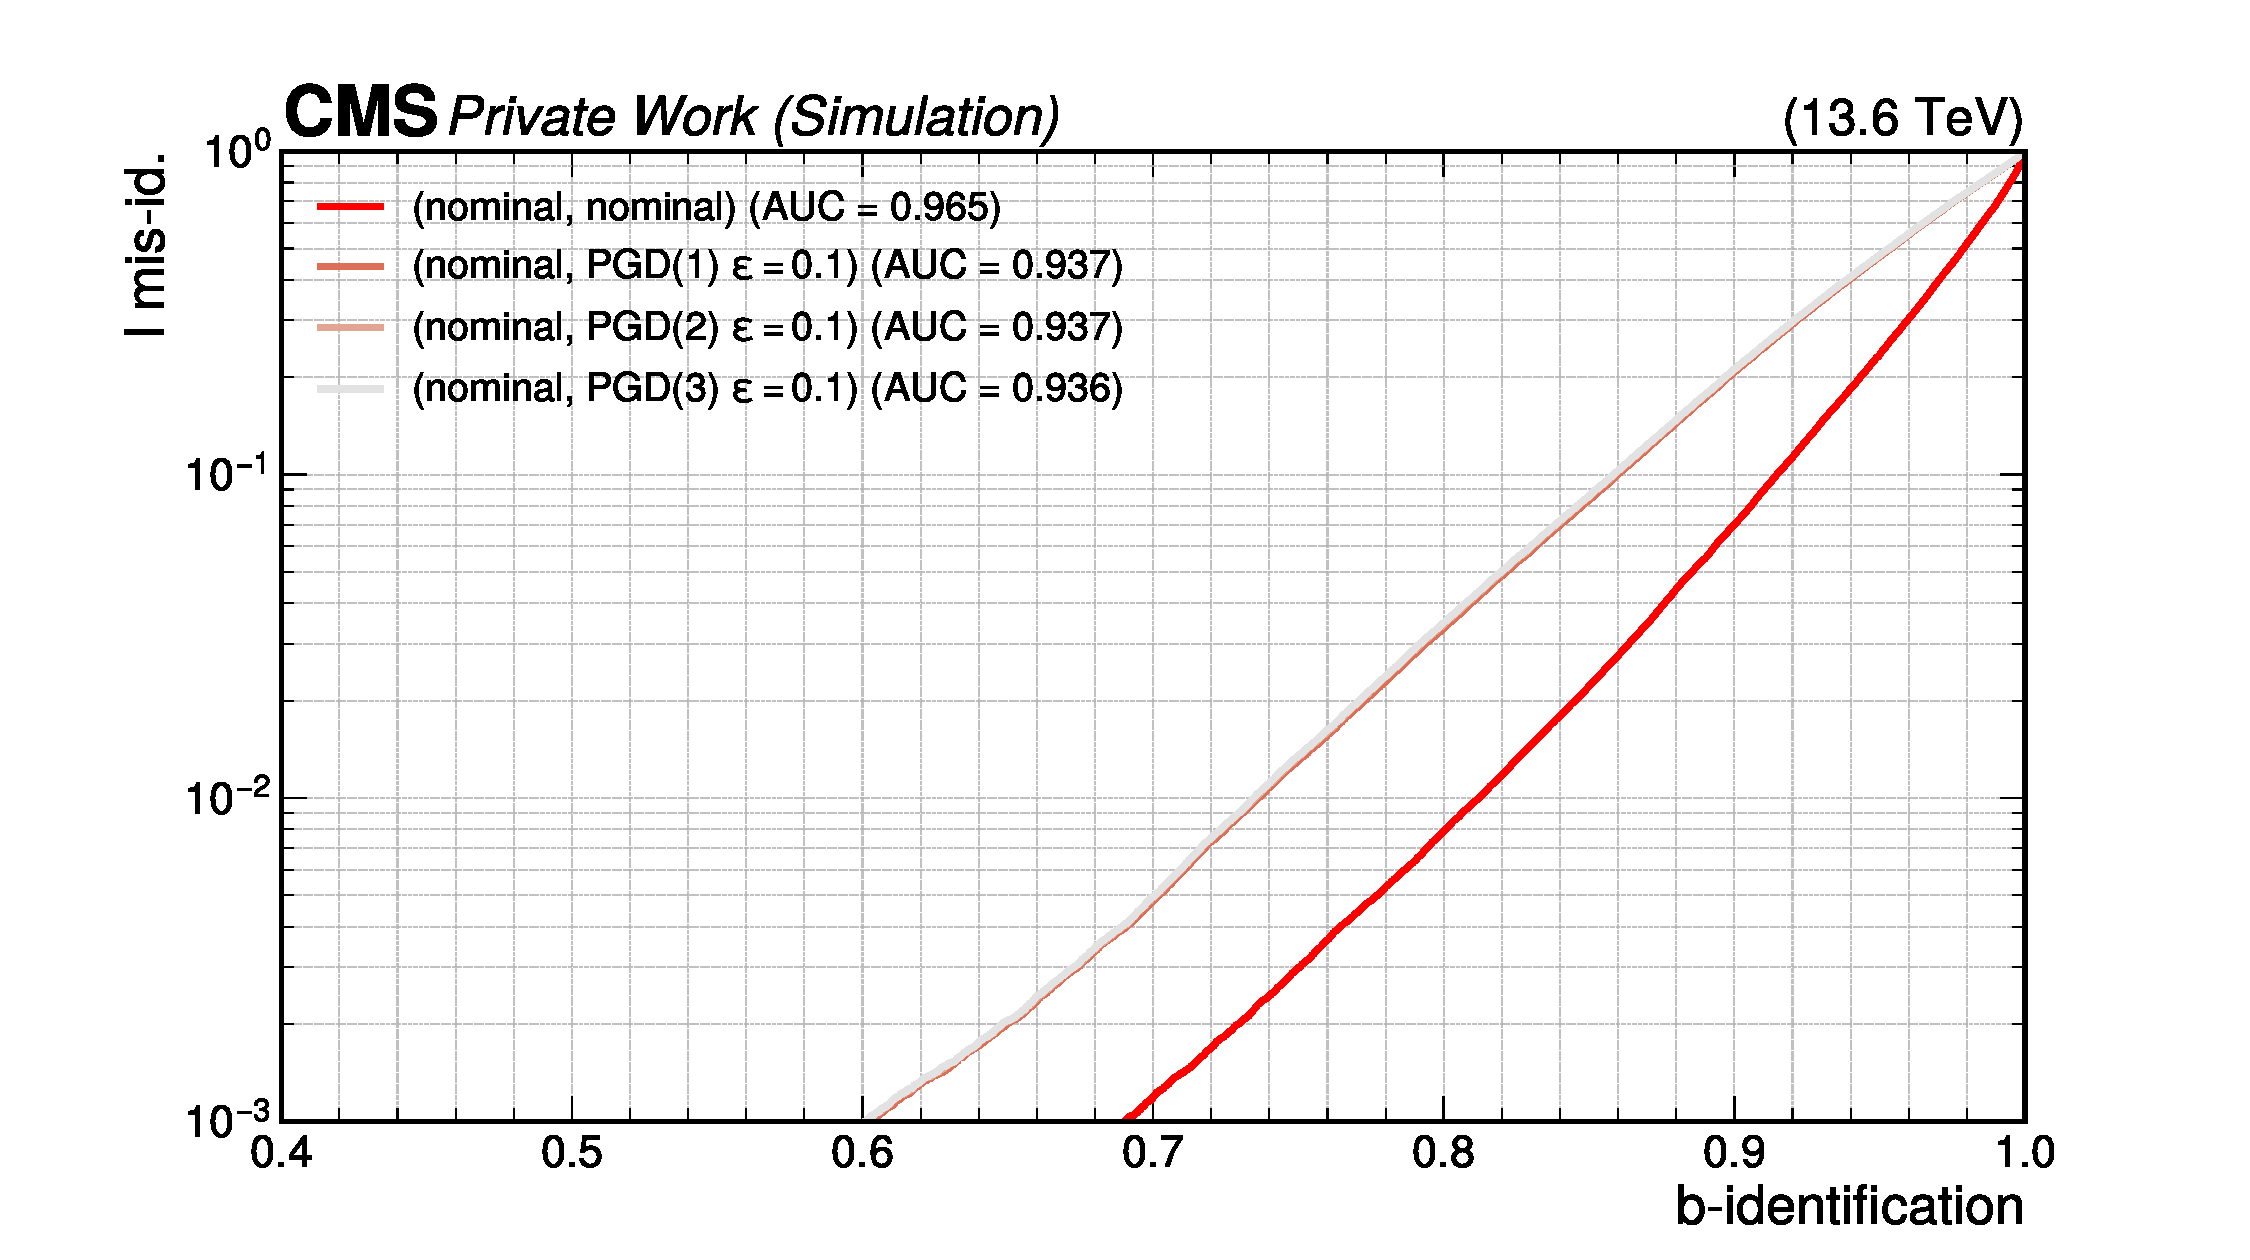
\includegraphics[width=15cm]{media/output/roc_bvsl_pgd_its_1_2_3.pdf}
    \caption{ROC curves for BvsL misidentification. Nominal trained model tested against one, two, and three iterations of PGD attacked inputs with $\epsilon=0.1$.}
    \label{fig:pgd_iterations}
\end{figure}

\paragraph{Adversarial Training:} Adversarial training with PGD perturbations introduces unique challenges to the learning process. The training and loss curve ( figure \ref{fig:pgd_loss_curve}) exhibit a higher spread between the convergence in loss (training sitting at approximately 1.0, validation at roughly 0.95), reflecting the inherent difficulty of learning robust representations under continuous adversarial perturbation. This is caused due to the necessity to simultaneously optimize for performance on clean data while developing defences against gradient-based attacks.

Notably, the training process achieves stable convergence despite the adversarial component. This means that PGD-based adversarial training is a viable strategy for improving model robustness.

\begin{figure}[h]
\centering
    
    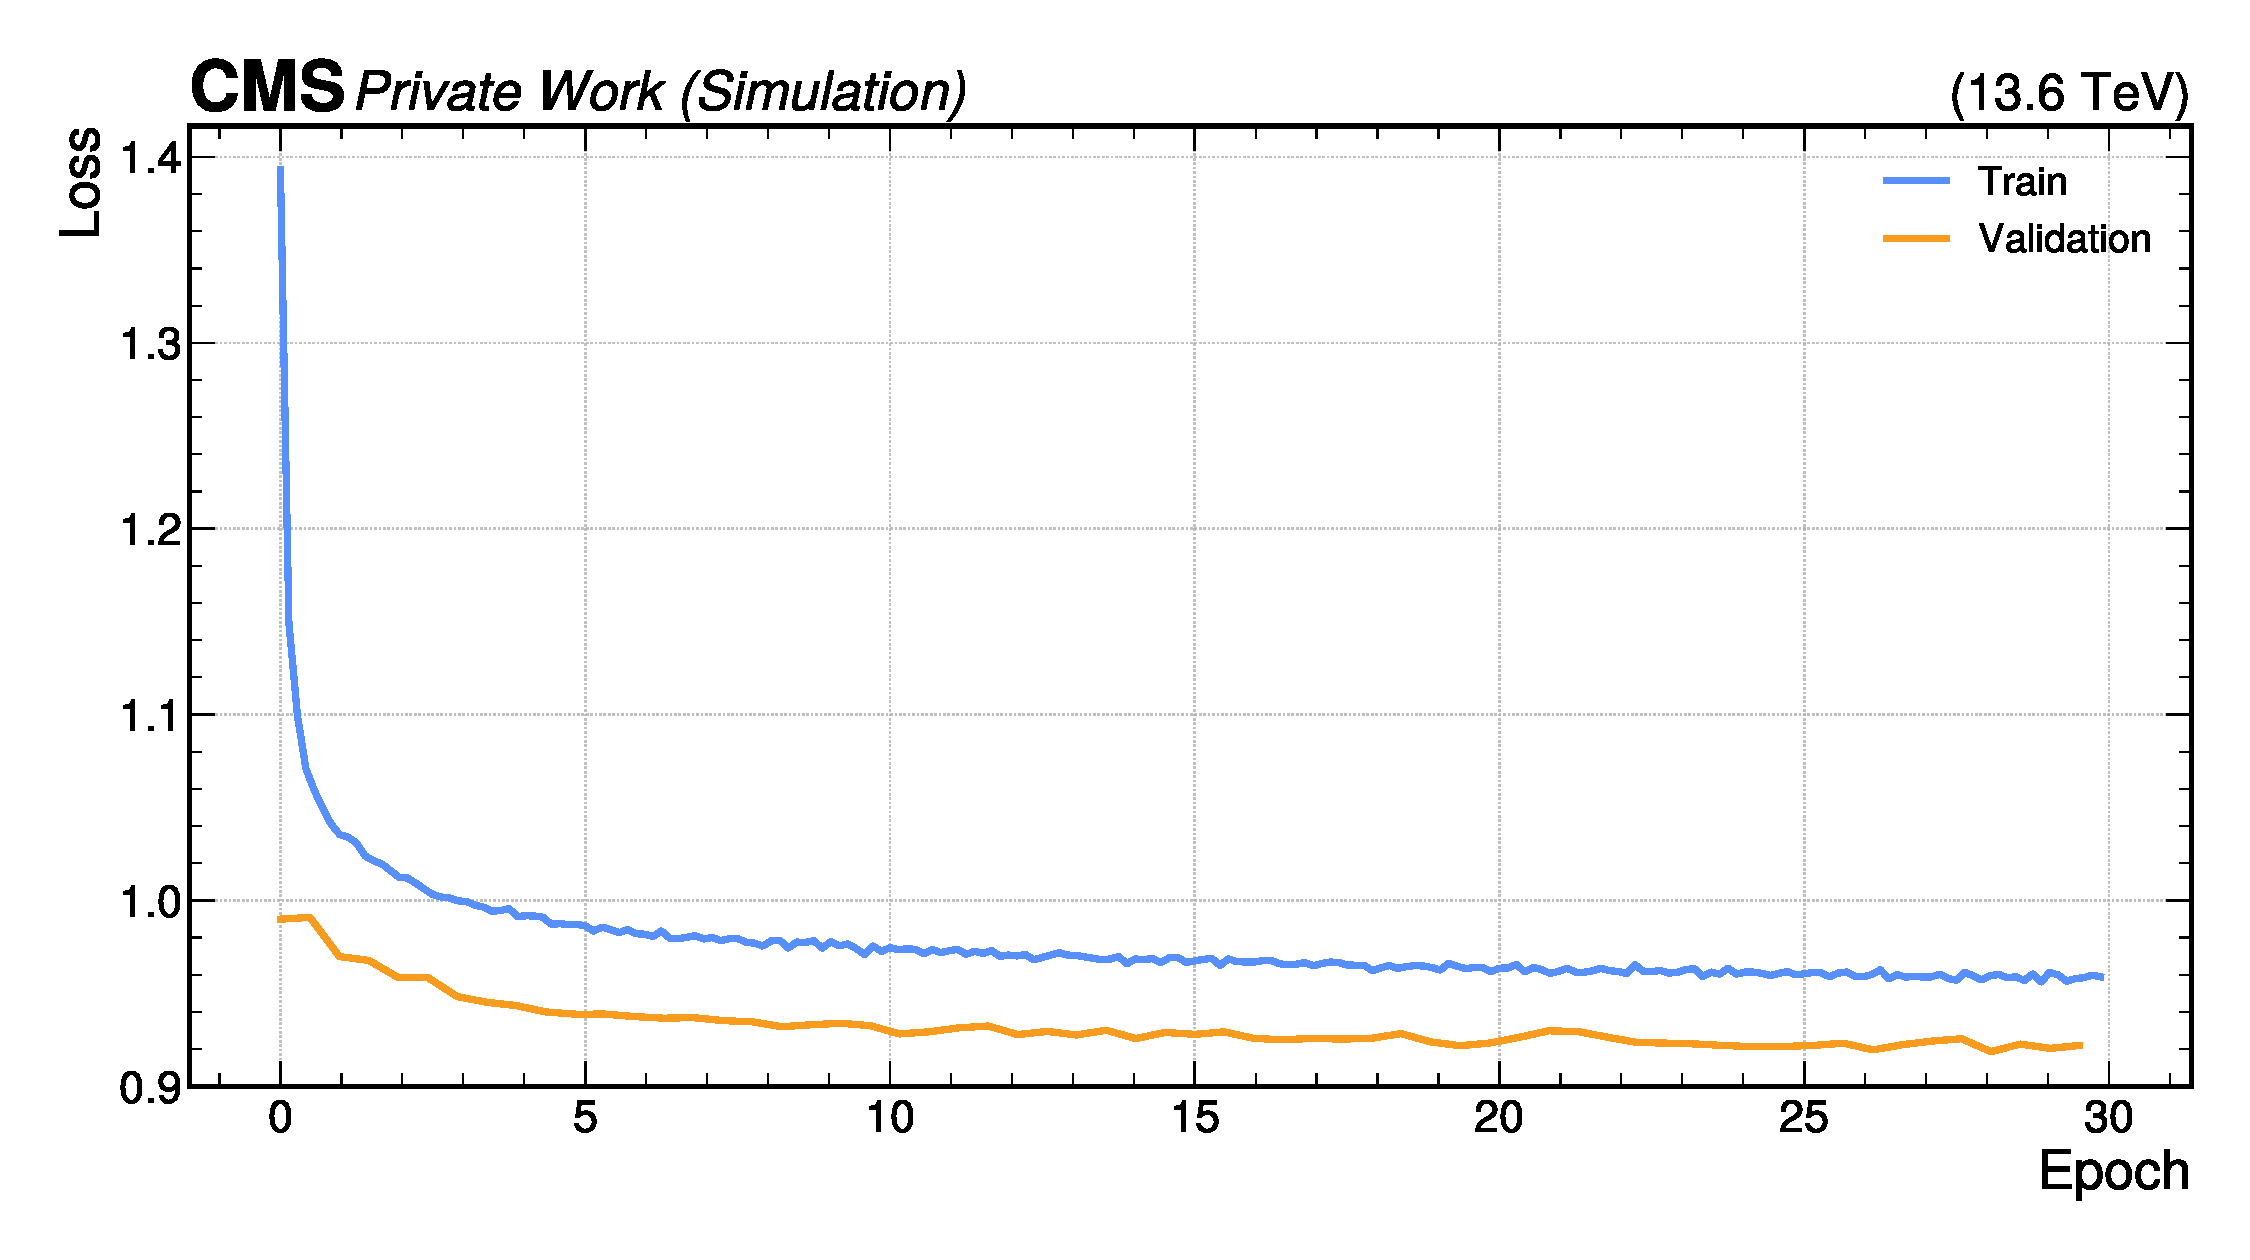
\includegraphics[width=15cm]{media/output/pgd_loss_validation.pdf}
    \caption{Training and validation loss for a PGD(1) trained model with a magnitude of $\epsilon=0.1$ for up to 30 epochs.}
    \label{fig:pgd_loss_curve}
\end{figure}

A PGD trained model offers robustness across PGD inferred data ($AUC=0.955$), while remaining a high AUC score for nominal data ($AUC=0.960$). Compared to the nominal trained model against PGD ($AUC=0.937$), it offers effective defence while staying true nominal performance of ($AUC=0.955$). The corresponding ROC curves are depicted in figure \ref{fig:pgd_trained}. 

\begin{figure}[h]
\centering
    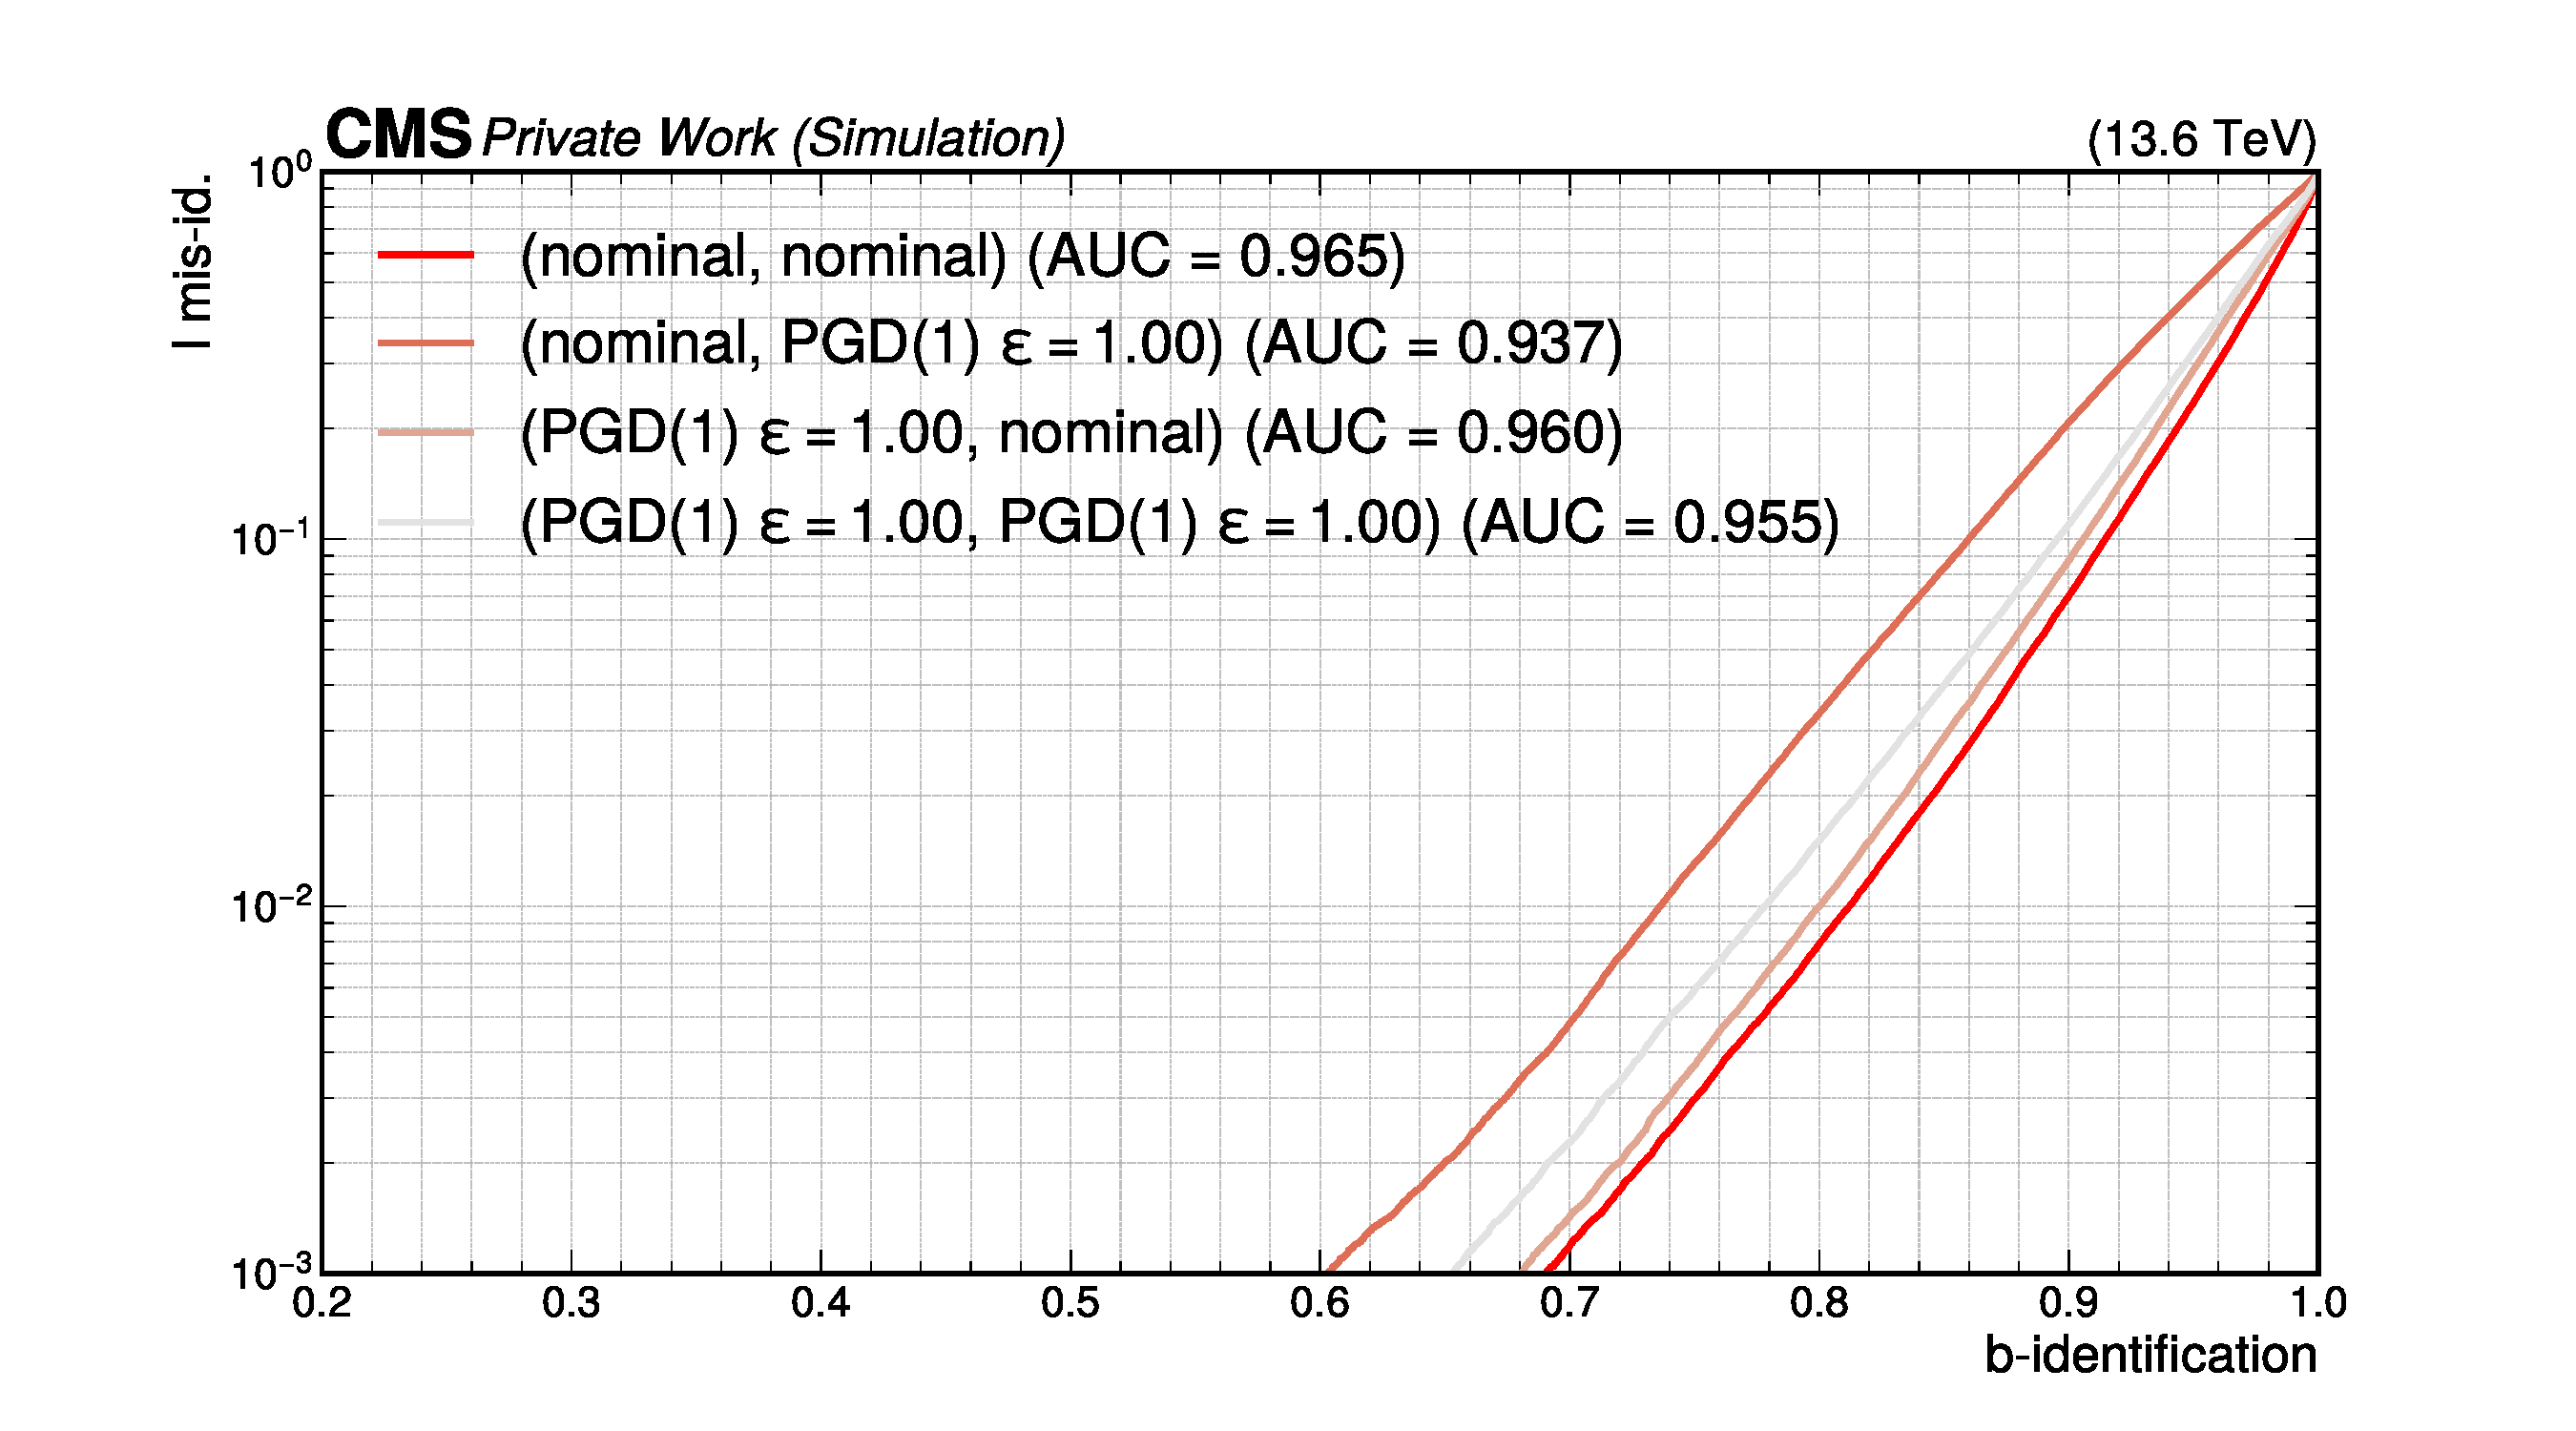
\includegraphics[width=15cm]{media/output/roc_bvsl_pgd_perms.pdf}
    \caption{ROC curves for BvsL misidentification for a PGD(1) and nominal trained model tested against nominal or PGD(1) perturbed inputs with a magnitude of $\epsilon=0.1$.}
    \label{fig:pgd_trained}
\end{figure}

\FloatBarrier
% PIP
\section{Probabilistic Integer Perturbation}
\label{sec:inprob_result}

If not declared specifically a sharpness of $s=1$ is assumed throughout this section. This value was chosen as it represents a compromise between nominal performance and a full-blown attack (see section \ref{sec:intprob_variability} for more details).

\paragraph{Severity:} The stealth characteristics of PIP attacks are fundamentally different from continuous perturbation methods due to their discrete nature. Figures \ref{fig:intprob_joint_overview} illustrates the perturbation severity over the targeted input domain. A comprehensive list of histograms for the input similarity of all features is provided in the Appendix \ref{appendix:intprob}.

The JSD analysis reveals that PIP perturbations maintain higher characteristics compared to PGD, with divergence values typically in the range of $\mathcal{O}(10^{-2})$ and some values going as far as $\mathcal{O}(10^{-1})$. These values occur as PIP is inherently discrete and its impact is generally dependent on the value range of each feature (e.g. for features such as \texttt{Npfcan\_isGamma} — a boolean flag — flipping a bit corresponds to a 100\% change in the respective input domain).

The comparison of single and double-iteration for PIP attacks — as seen in figures \ref{fig:intprob_severity_npv} and \ref{fig:intprob_severity_vtxAss} — indicates a relatively minimal difference in perturbation severity.

\begin{figure}[h]
\centering
    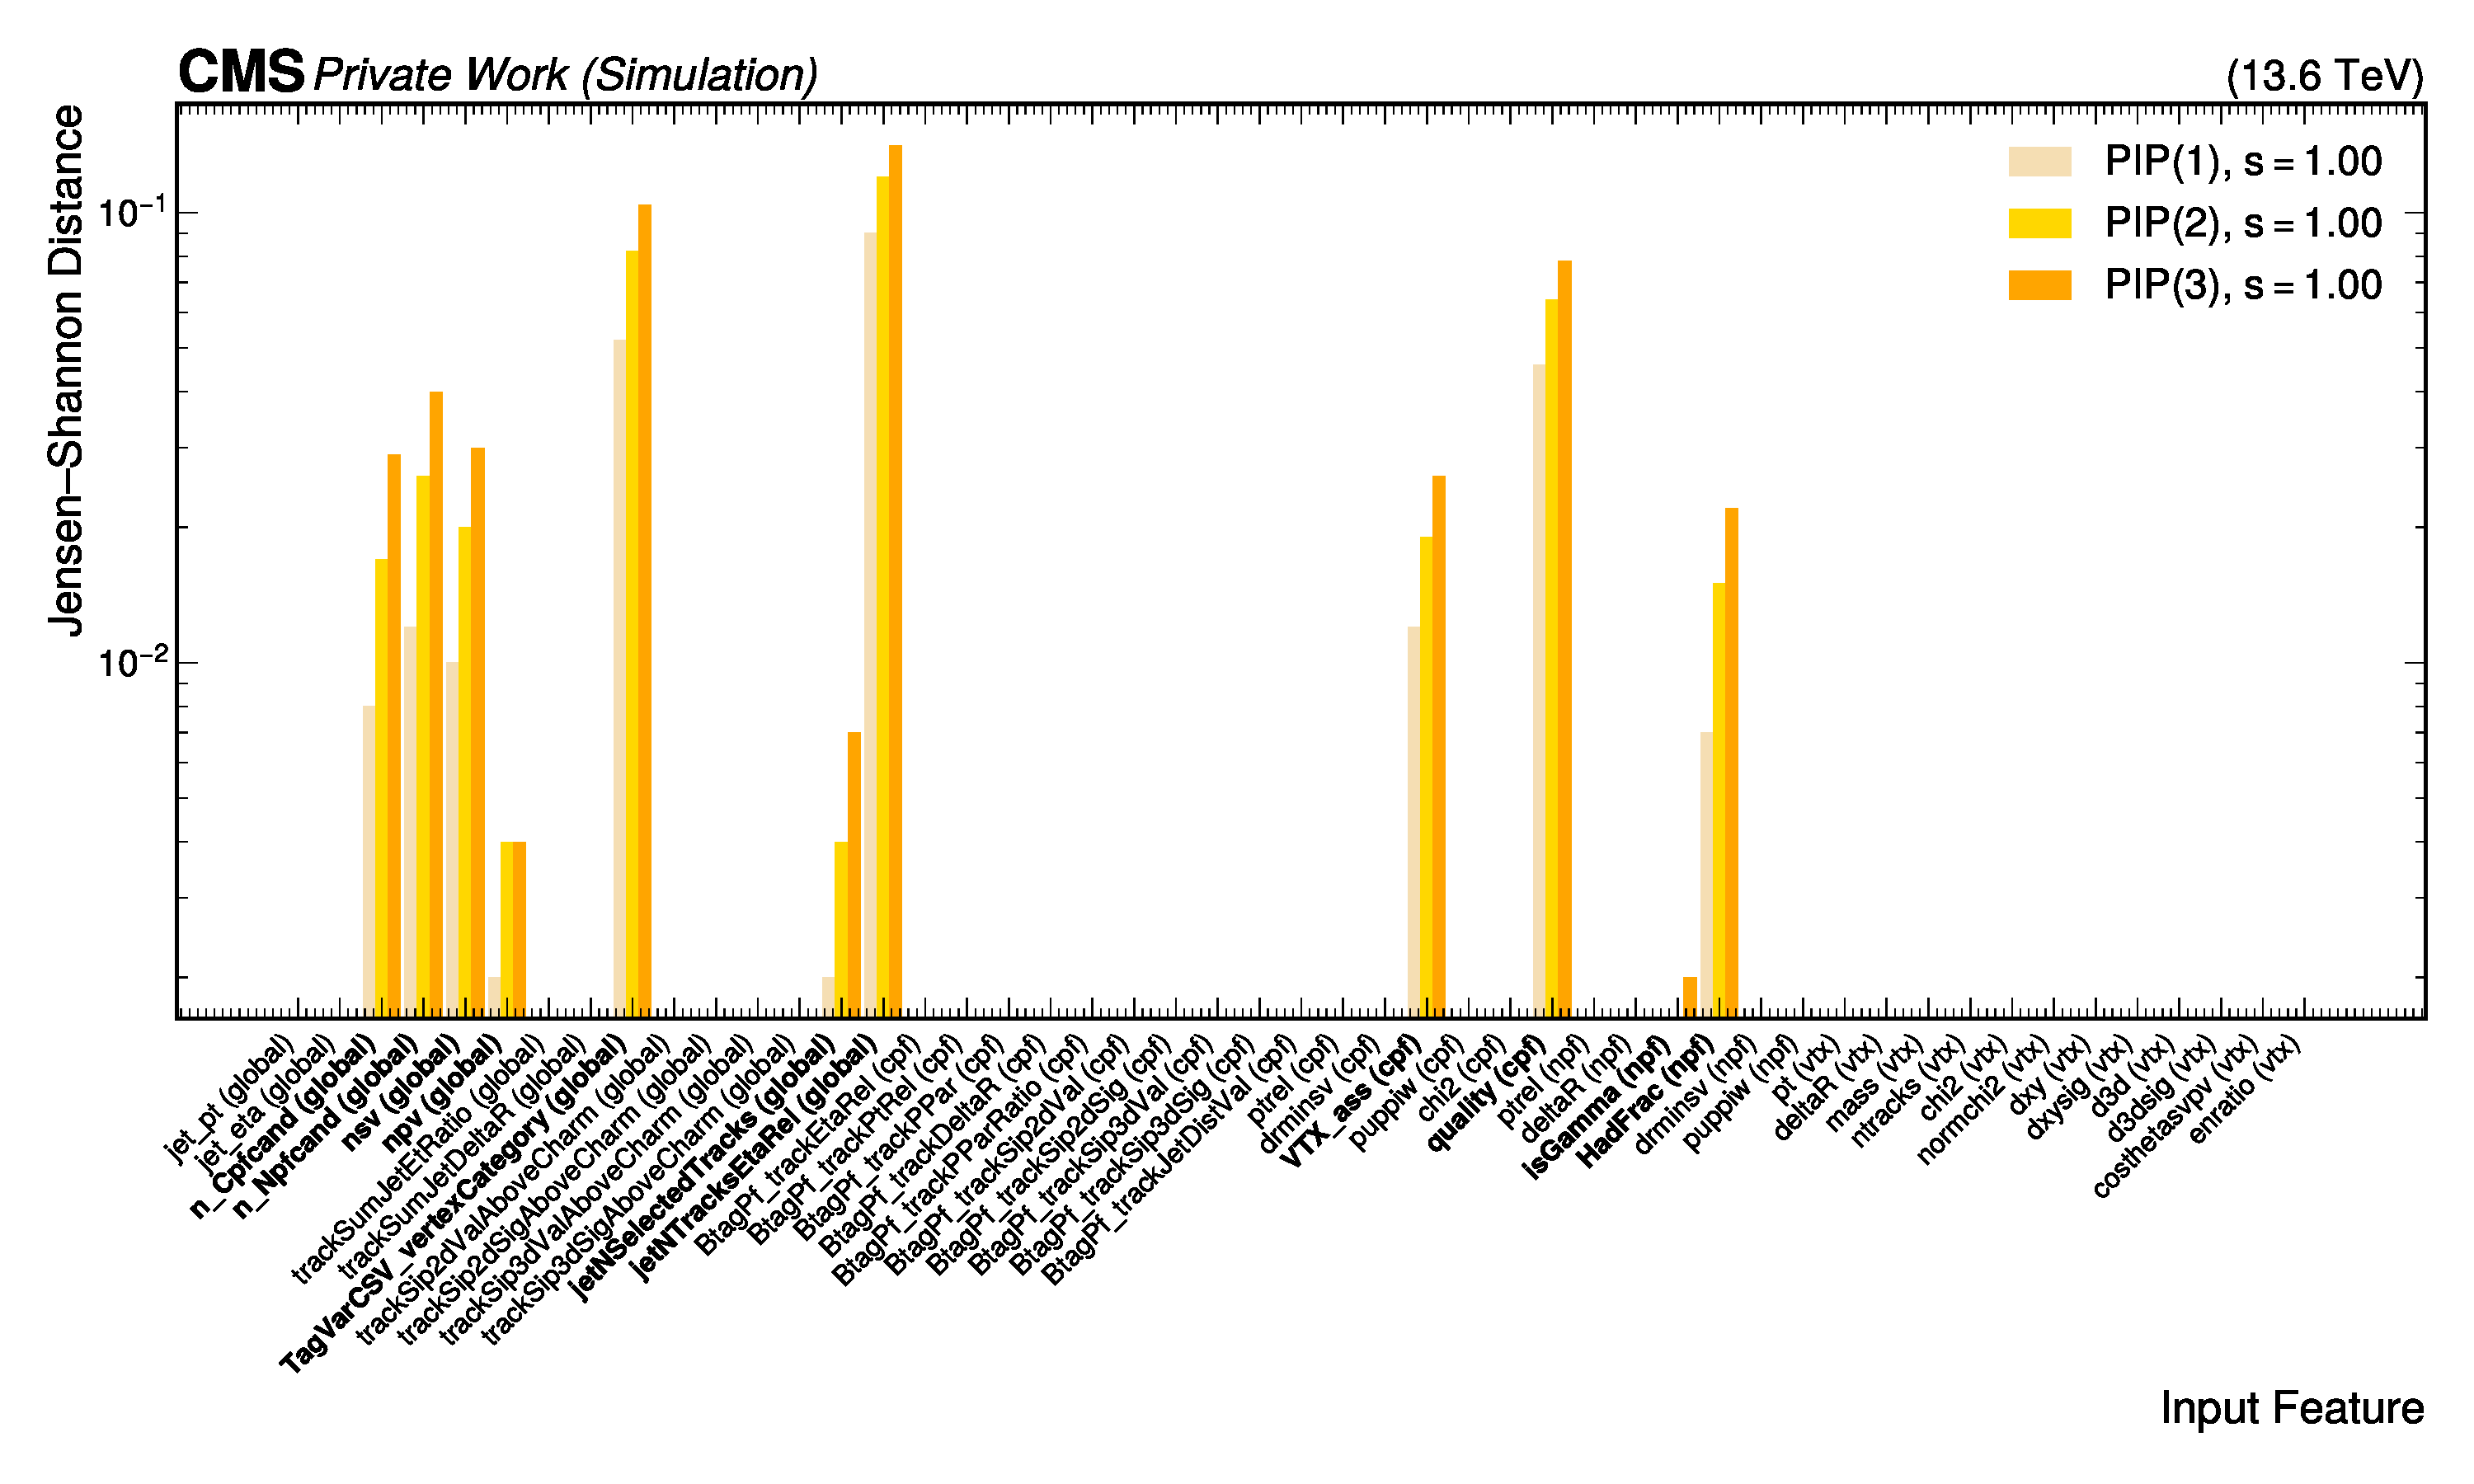
\includegraphics[width=15cm]{media/output/features/compare/jsd_intprob_per_feature.pdf}
    \caption{JSD input similarity development for up to three iterations of the PIP attack with $s=1$ compared against a nominal trained model.}
    \label{fig:intprob_joint_overview}
\end{figure}

\begin{figure}[htbp]
  \centering
  \begin{subfigure}[t]{0.5\textwidth}
    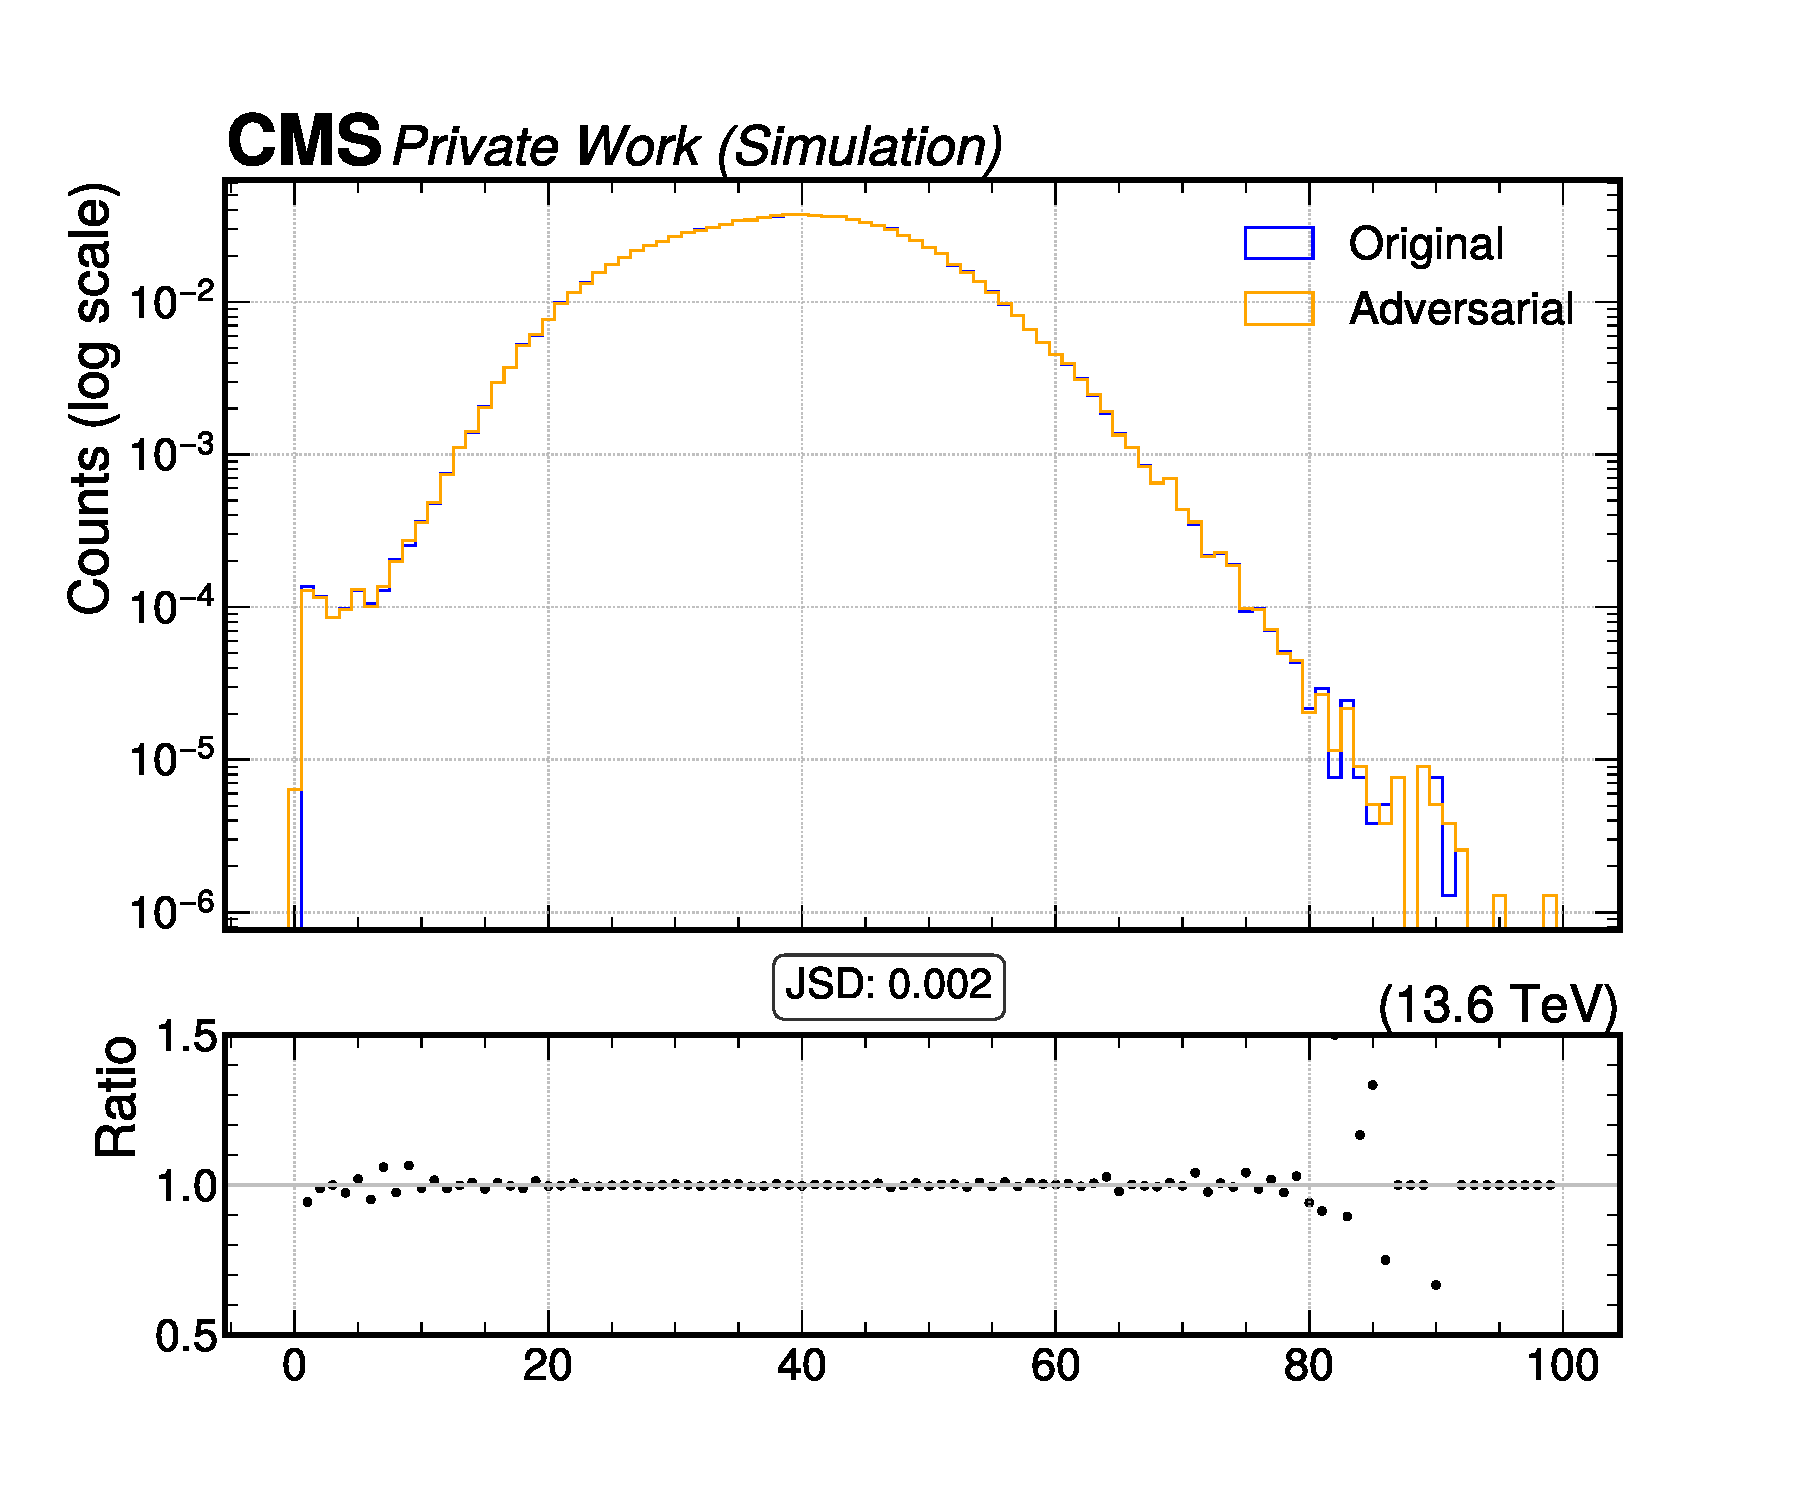
\includegraphics[width=\linewidth]{media/output/features/compare/intprob_1/cmp_global_features_npv.pdf}
    \caption{Input similarity for PIP(1).}
    \label{fig:left}
  \end{subfigure}\hfill
  \begin{subfigure}[t]{0.5\textwidth}
    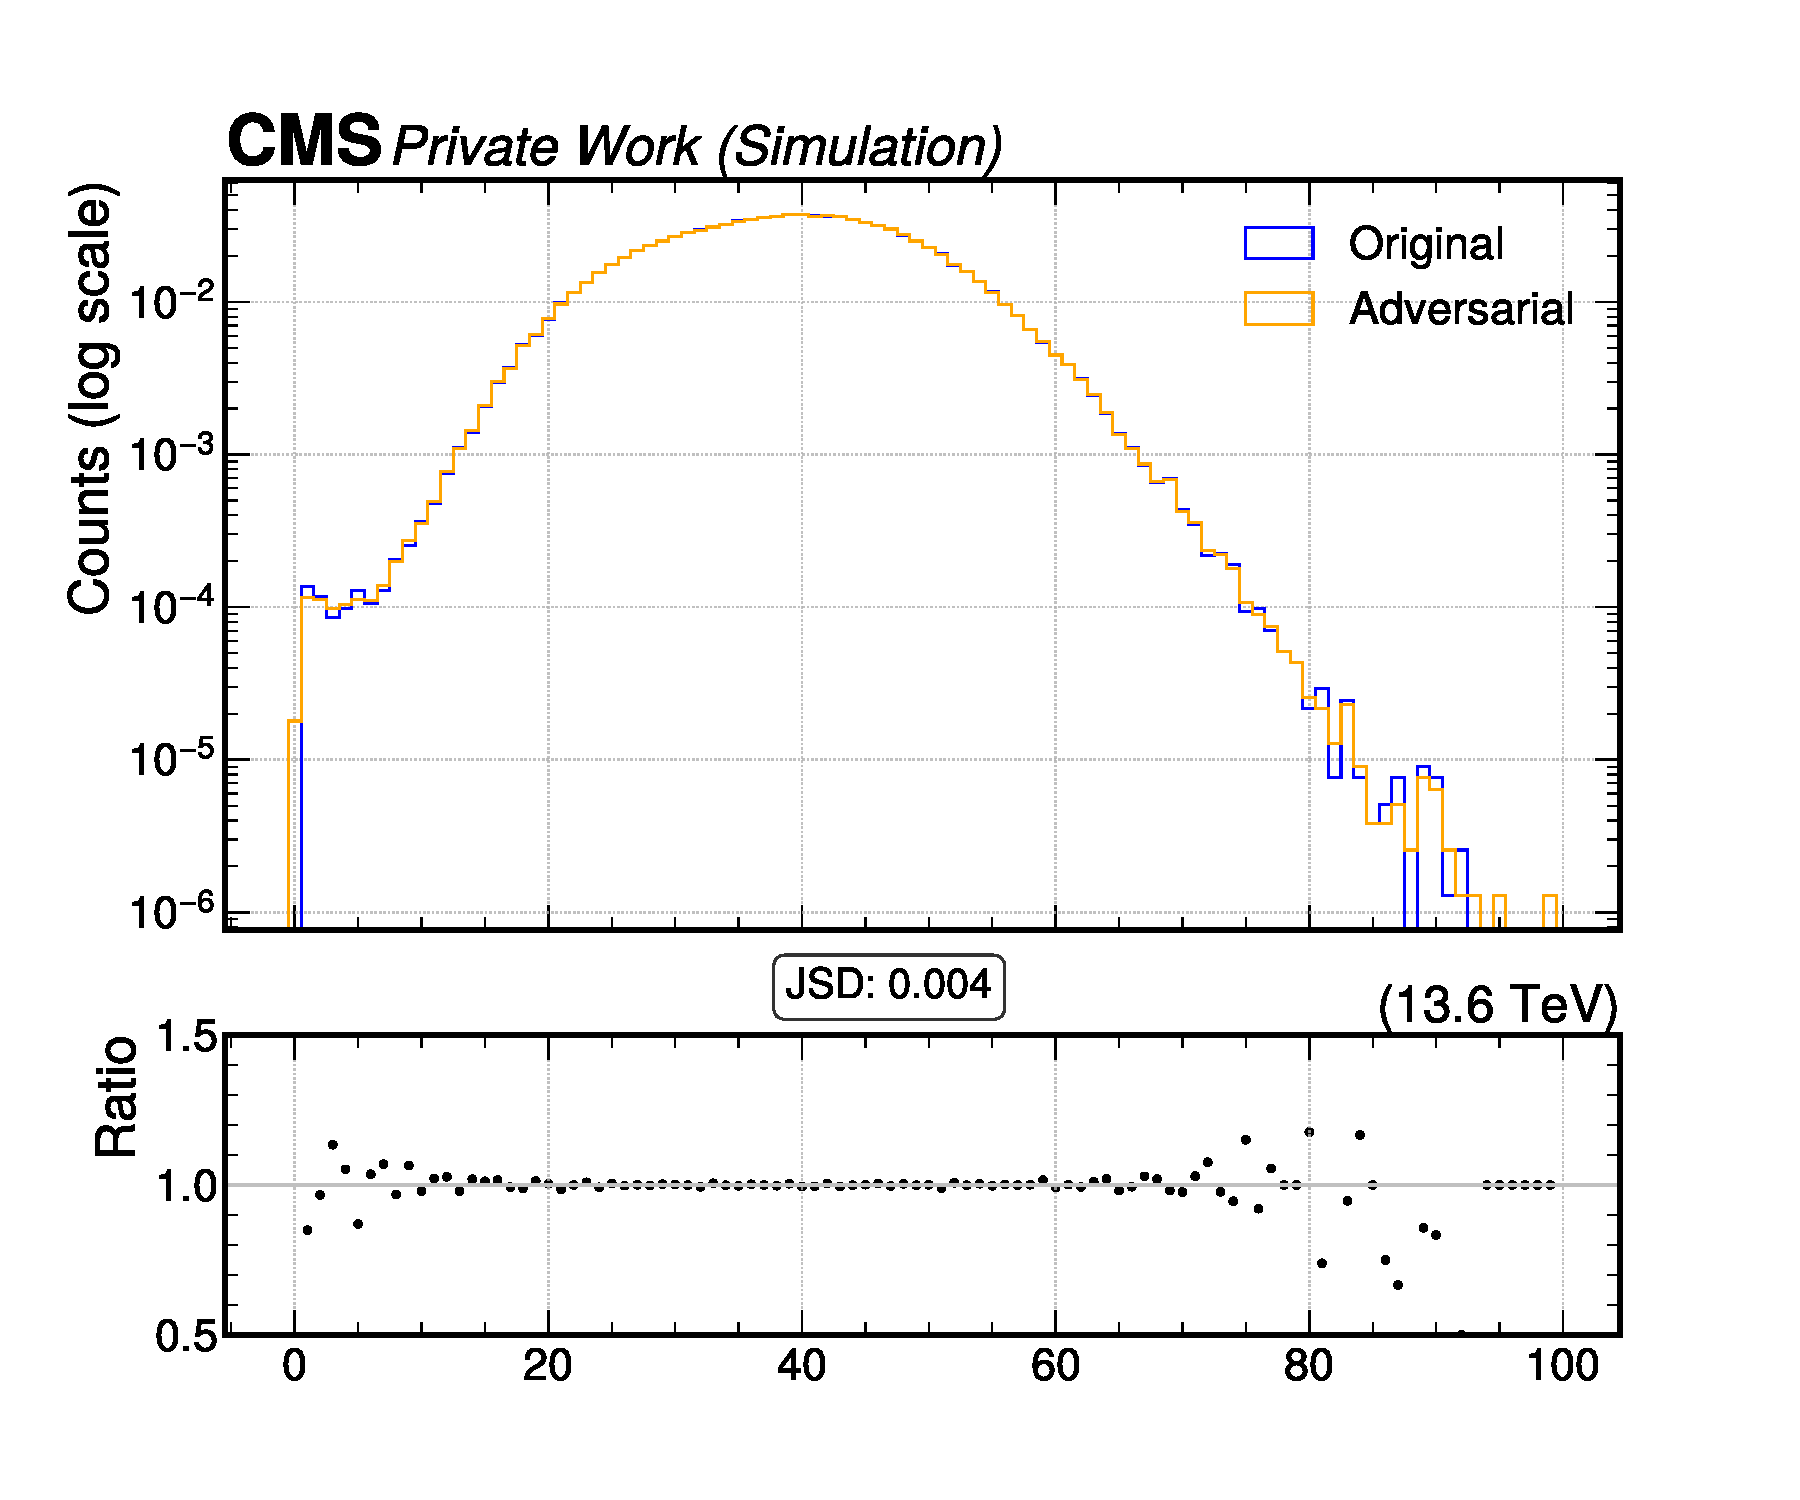
\includegraphics[width=\linewidth]{media/output/features/compare/intprob_2/cmp_global_features_npv.pdf}
    \caption{Input similarity for PIP(2).}
  \end{subfigure}\hfill

  \caption{Histogram for global \texttt{npv} for one and two iterations (left and right respectively) of PIP with a sharpness of $s=1$ compared against nominal inputs.}
  \label{fig:intprob_severity_npv}
  
  \begin{subfigure}[t]{0.5\textwidth}
    \includegraphics[width=\linewidth]{media/output/features/compare/intprob_1/cmp_global_features_nsv.pdf}
    \caption{Input similarity for PIP(1).}
    \label{fig:left}
  \end{subfigure}\hfill
  \begin{subfigure}[t]{0.5\textwidth}
    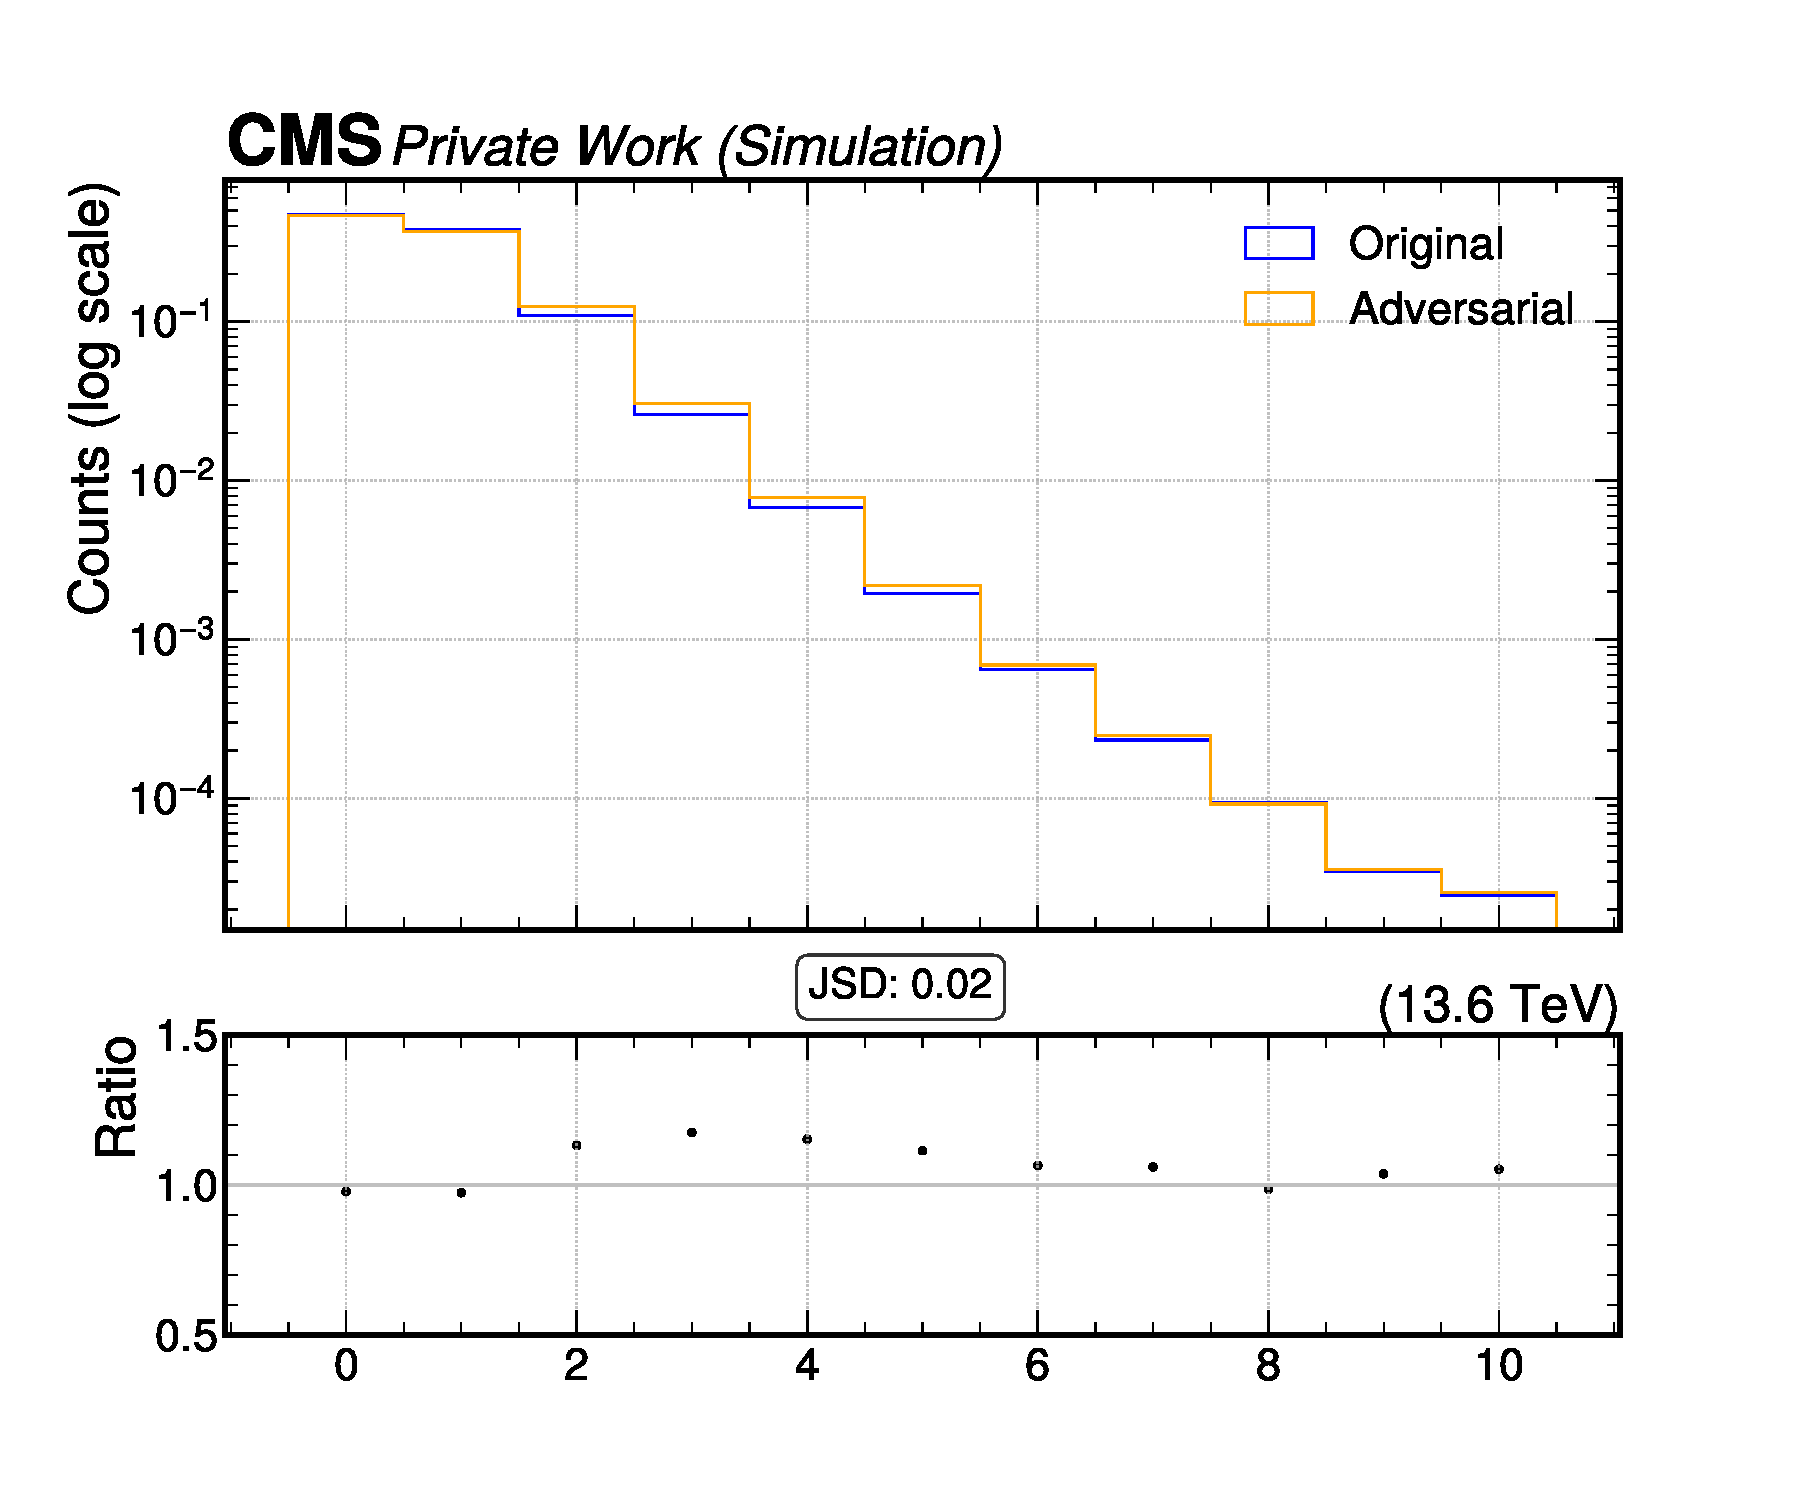
\includegraphics[width=\linewidth]{media/output/features/compare/intprob_2/cmp_global_features_nsv.pdf}
    \caption{Input similarity for PIP(2).}
  \end{subfigure}\hfill

  \caption{Histogram for global \texttt{nsv} for one and two iterations (left and right respectively) of PIP with a sharpness of $s=1$ compared against nominal inputs.}
  \label{fig:intprob_severity_vtxAss}
\end{figure}

\newpage
\paragraph{Attack:} The PIP attack exhibits a distinct characteristic compared to PGD. Its effectiveness depends on the number of iterations and the sharpness parameter in roughly same parts. Figure \ref{fig:intprob_rocs_vs_sharpness} illustrates this relationship, showing how varying sharpness values affect the attack's ability to compromise the classifier:

\begin{figure}[H]
\centering
    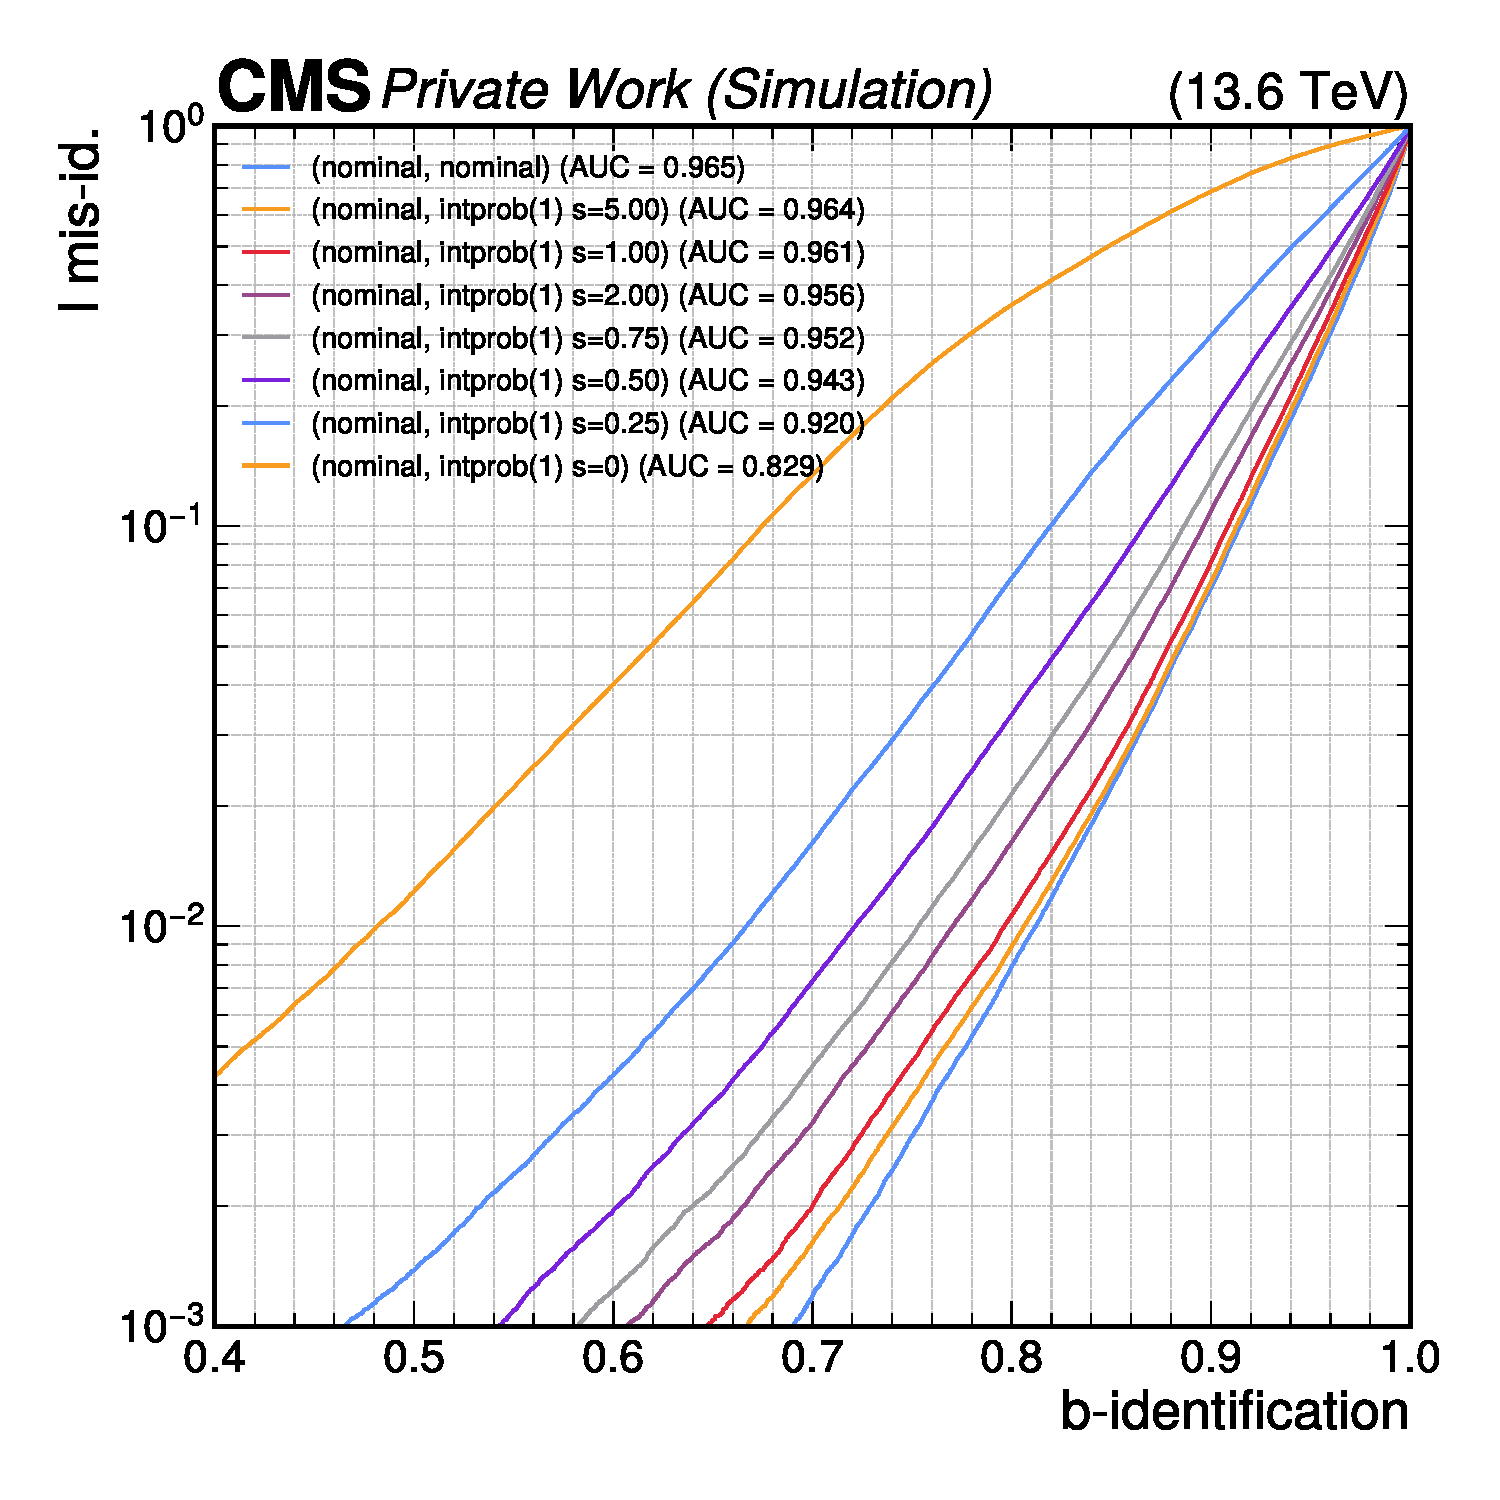
\includegraphics[width=15cm]{media/output/roc_bvsl_intprob_sharpness.pdf}
    \caption{ROC curves for BvsL misidentification of the nominal trained model tested against different sharpness values for the PIP attack at one iteration.}
    \label{fig:intprob_rocs_vs_sharpness}
\end{figure}

\begin{itemize}
    \item At \textbf{high sharpness} ($s = 5$), the attack exhibits minimal impact, with AUC values remaining close to the nominal baseline. This reflects the probabilistic nature of the PIP method—when the sharpness is high, the probability of flipping integer features remains small, resulting in perturbations that are too subtle to significantly affect the classifier's decision boundaries.
    \item At \textbf{moderate sharpness} around $s = 1.0$, a more pronounced degradation becomes apparent, with the AUC dropping to approximately 0.961. This represents the sweet spot where the attack achieves meaningful perturbation while maintaining reasonable stealth characteristics. 
    \item A \textbf{low sharpness} of $s = 0$ corresponds to a completely deterministic attack, where all features with a gradient unequal to zero get eventually increased/decreased. It produces the most aggressive attack, reaching an AUC of around 0.829.
\end{itemize}


Likewise, figure \ref{fig:intprob_rocs_vs_iterations} highlights PIP's iterative behaviour. Unlike PGD, where additional iterations yield progressively smaller changes, PIP exhibits steady AUC degradation, with subsequent iterations reducing the AUC from 0.956 at one iteration to 0.916 at five iterations. This behaviour arises from PIP's stochastic nature, where features unaltered in prior iterations gain further opportunities for modification in later ones. This increases their cumulative perturbation probability across iterations.


\begin{figure}[h]
\centering
    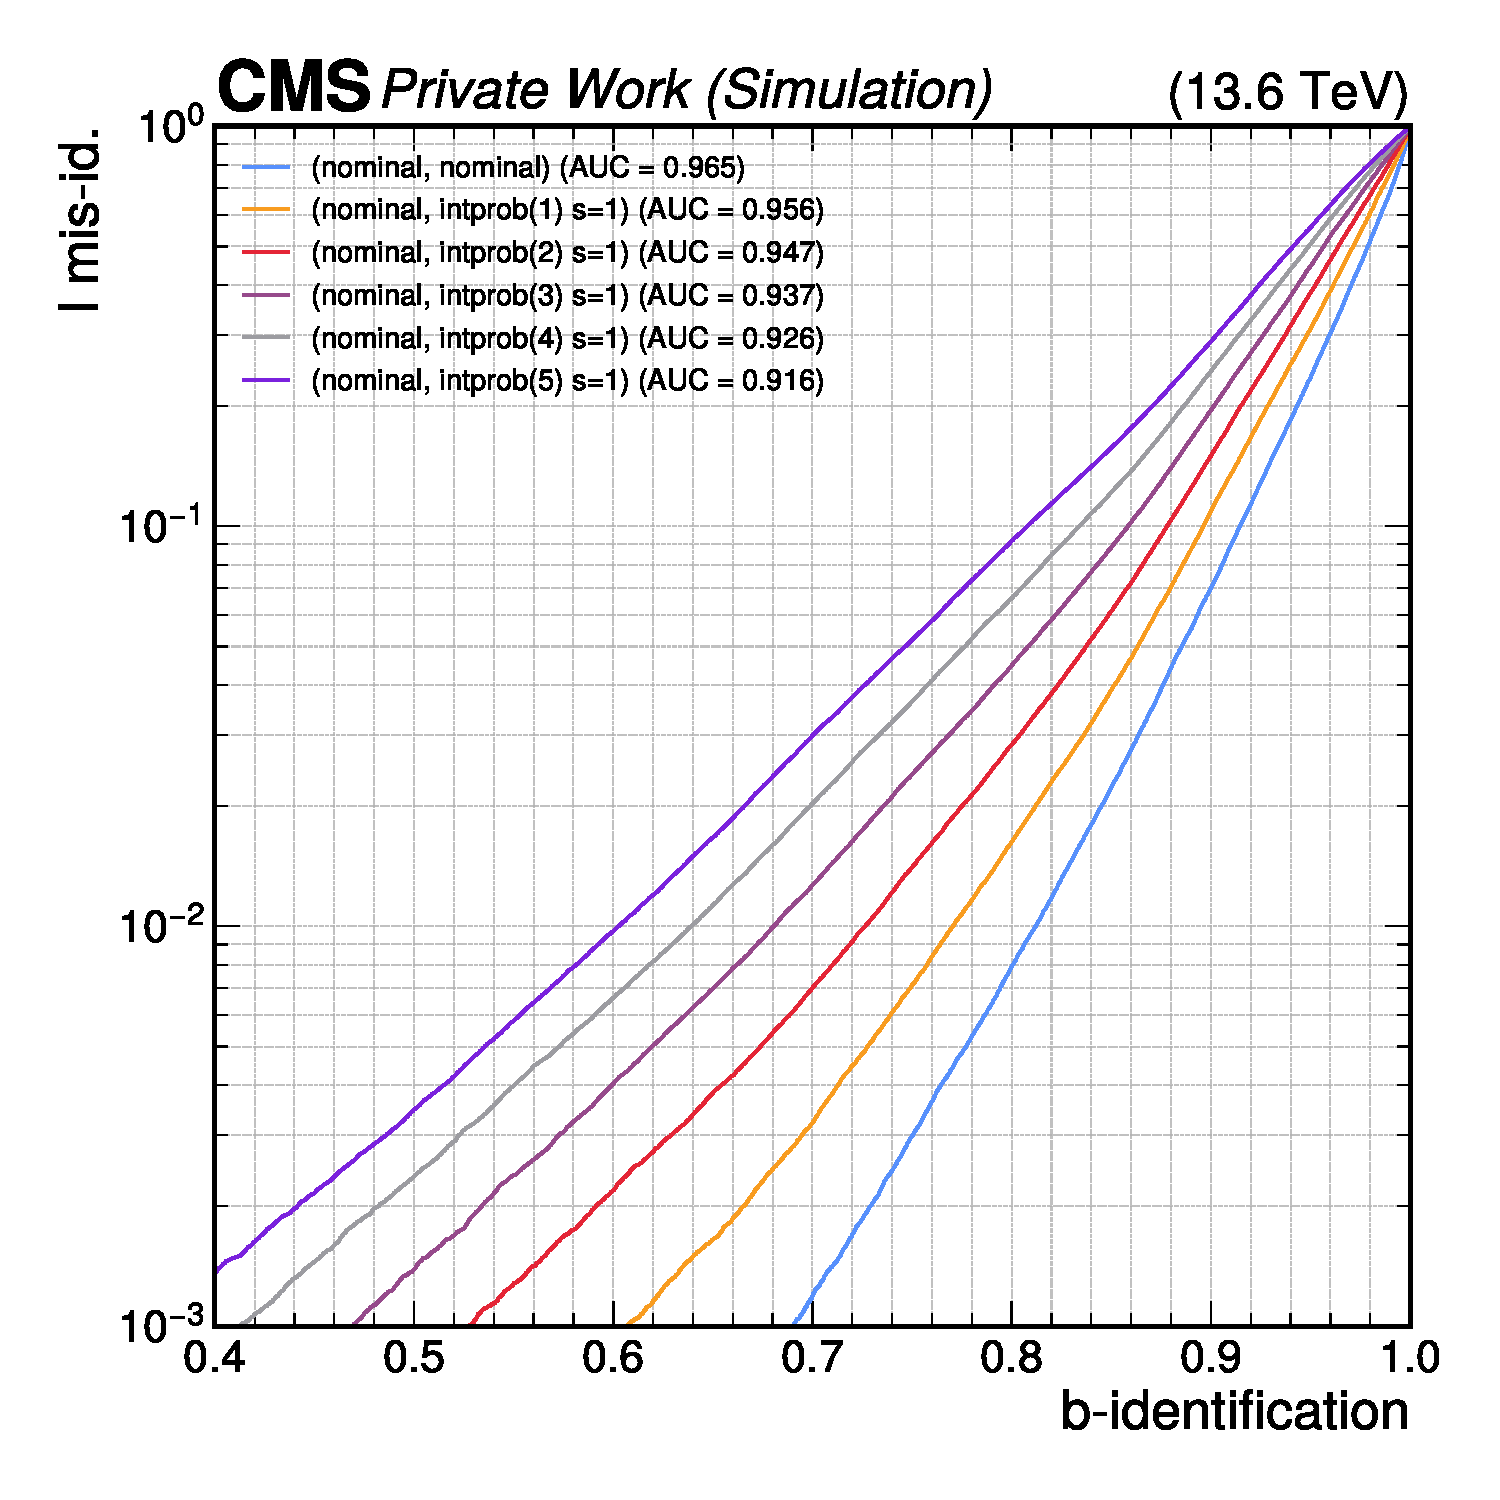
\includegraphics[width=15cm]{media/output/roc_bvsl_intprob_iterations.pdf}
    \caption{ROC curve for BvsL misidentification of the nominal trained model tested against up to five iteration of the PIP attack at $s=1$.}
    \label{fig:intprob_rocs_vs_iterations}
\end{figure}

\paragraph{Adversarial Training:} PIP's adversarial training presents a distinct learning scenario compared to continuous perturbation methods. 
Figure \ref{fig:intprob_training} shows the training dynamics for PIP with sharpness $s=1$ over 30 epochs, revealing several interesting characteristics of discrete adversarial training.

\begin{figure}[h]
\centering
    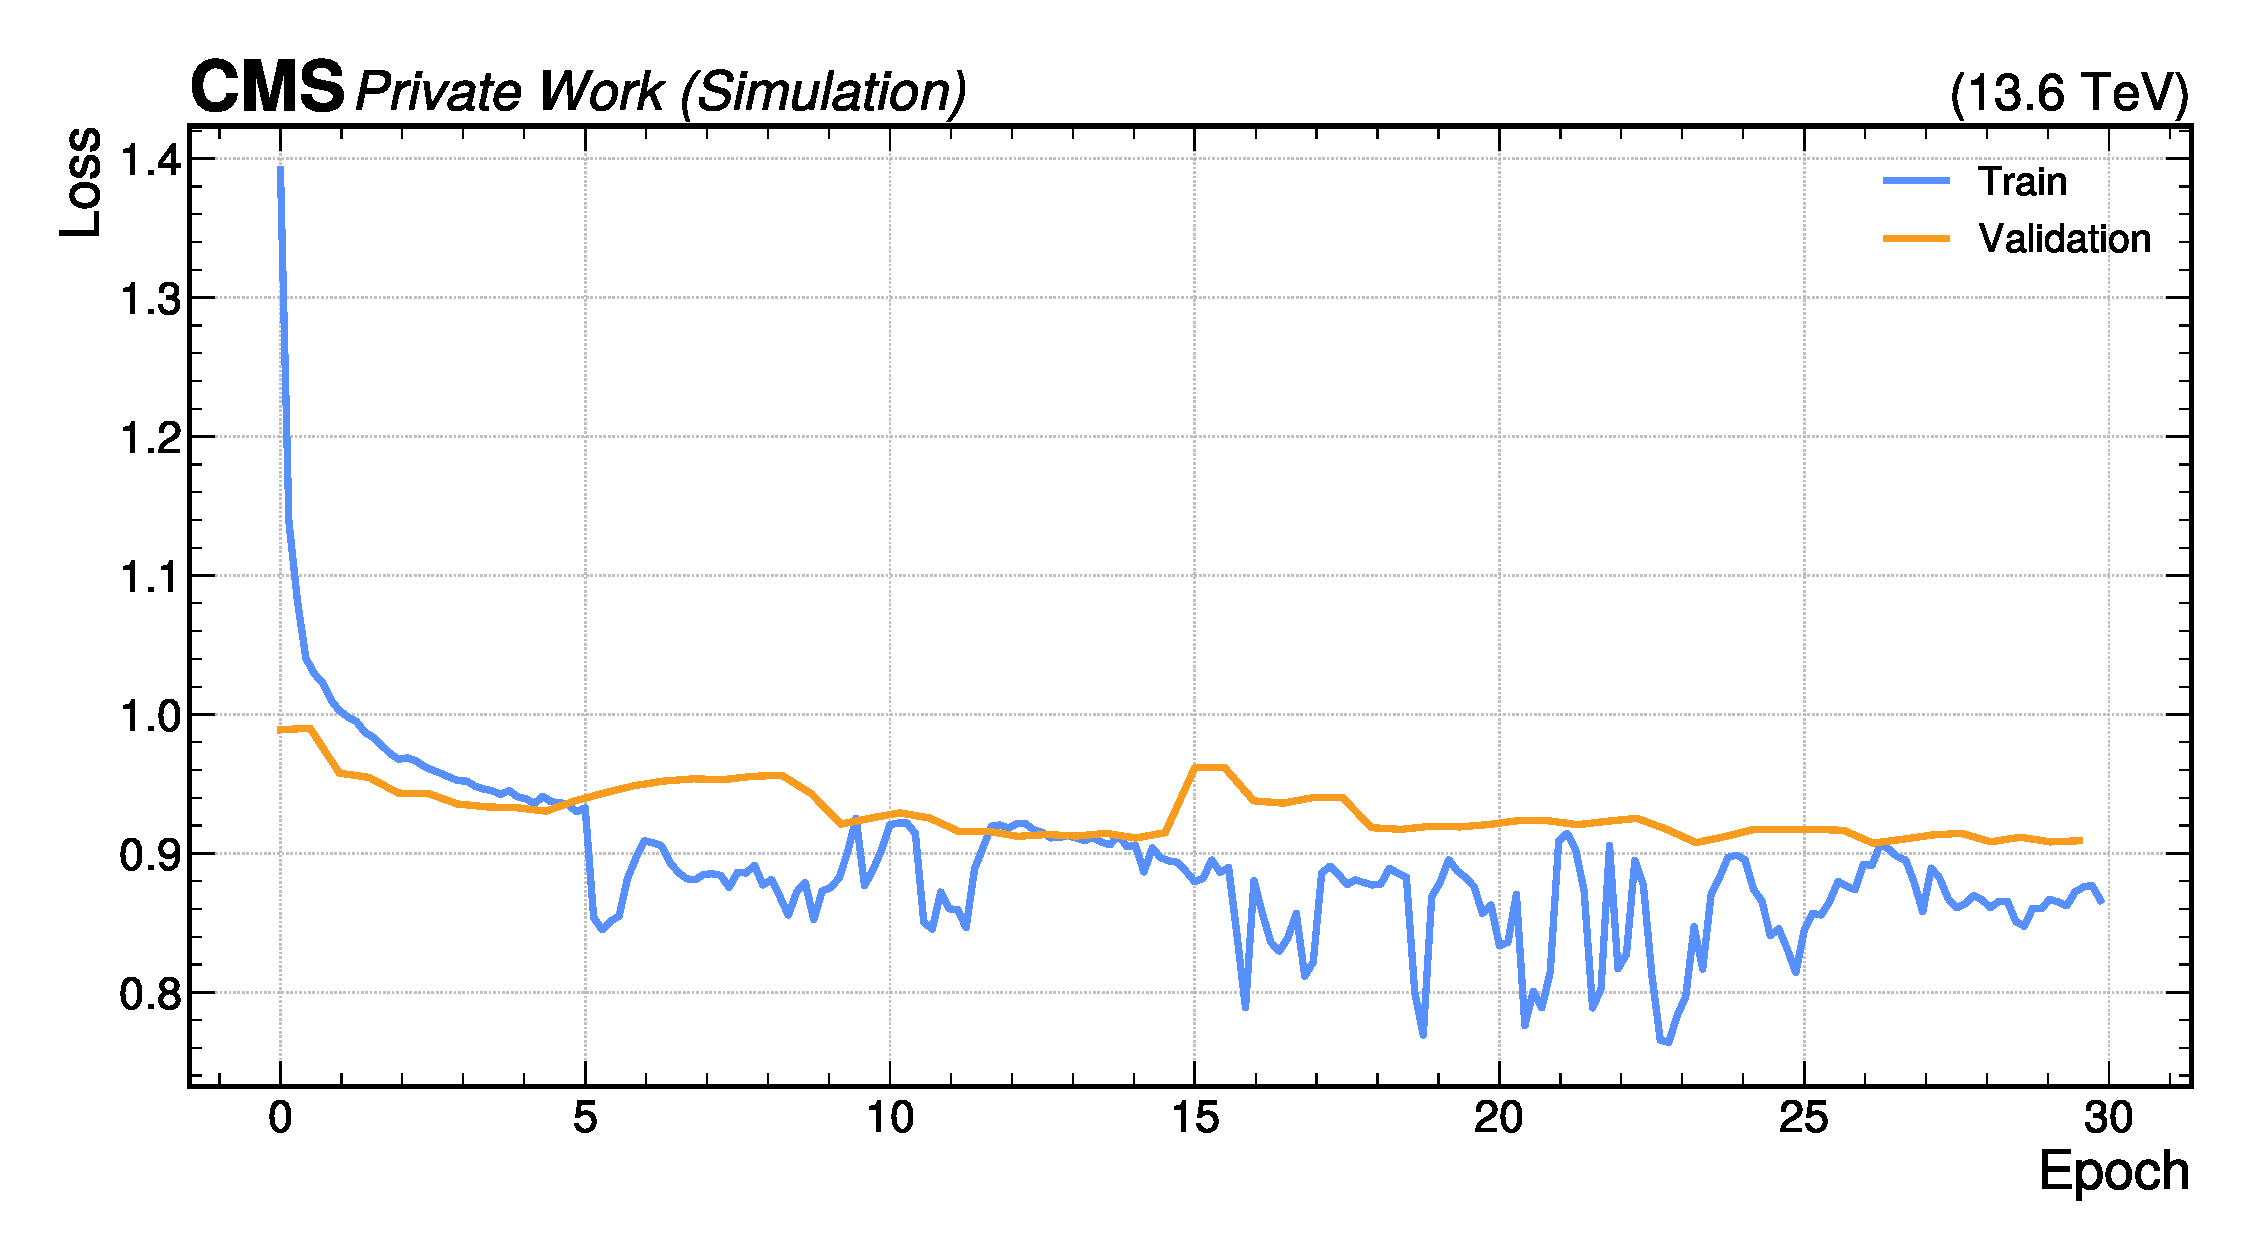
\includegraphics[width=15cm]{media/output/intprob_loss_validation.pdf}
    \caption{Training and validation loss for a PIP trained model over 30 epochs with a sharpness of 1.}
    \label{fig:intprob_training}
\end{figure}

The training loss curve demonstrates visible fluctuations, particularly in comparison to PGD-based training. This instability stems from the discrete nature of PIP perturbations — unlike continuous methods that can produce arbitrarily small perturbations, PIP operates on a finite set of possible integer modifications. This creates less but more pronounced perturbations offering a greater challenge in the training procedure. This instability reflects in the validation loss too, indicating problems to generalize for unseen PIP perturbations. Compared to nominal training or PGD, the validation loss slightly exceeds the training loss, suggesting mild adaptation to the lower-severity PIP perturbations \ref{fig:intprob_rocs_training}).

Figure \ref{fig:intprob_rocs_training} shows that the PIP-trained model achieves robust performance against PIP-perturbed data, with an AUC of $0.967$, slightly surpassing the nominal-trained baseline ($AUC = 0.965$) by approximately $0.2\%$. When evaluated on nominal data, the model maintains a strong AUC of $0.962$, indicating minimal performance degradation compared to the undisturbed model.

\begin{figure}[h]
\centering
    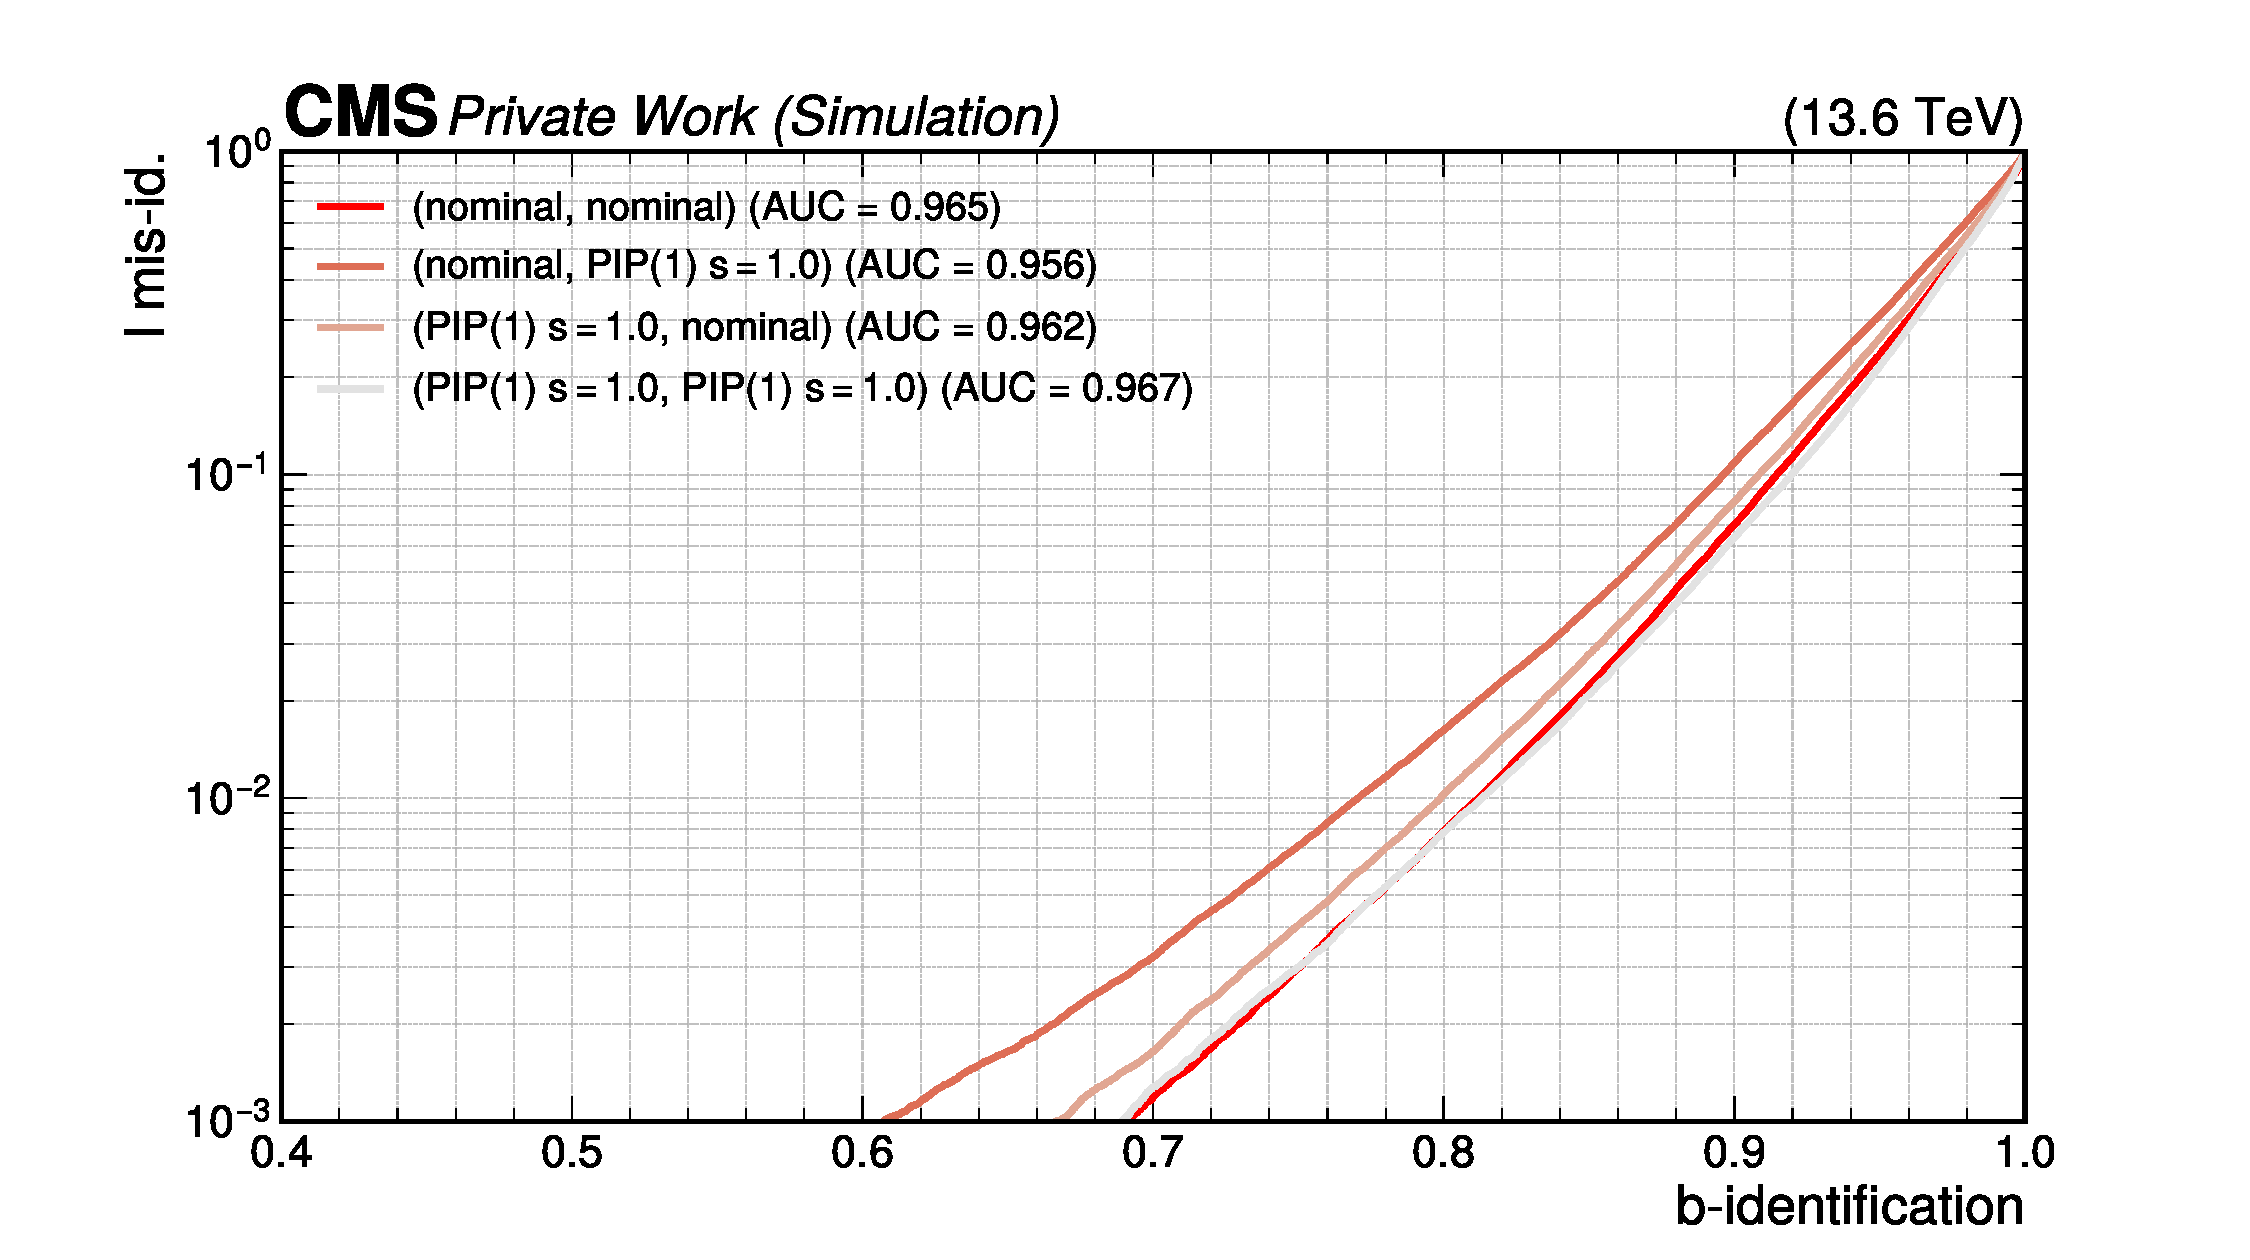
\includegraphics[width=15cm]{media/output/roc_bvsl_intprob_permutations.pdf}
    \caption{ROC curves for BvsL misidentification for a PIP(1) and nominal trained model tested against nominal or PIP(1) perturbed inputs with a sharpness of $s=1.0$.}
    \label{fig:intprob_rocs_training}
\end{figure}

\FloatBarrier
% Joint Application of PIP and PGD
\section{Probabilistic Integer-Perturbed Projected Gradient Descent}

As described in Sec.~\ref{sec:method_combined}, the PIP-PGD attack perturbs floating-point and integer features independently in a single pass. The following analysis examines its effect on input similarity, model performance, and training behaviour.

\paragraph{Severity:} The JSD analysis reveals that combined attacks retain stealth characteristics comparable to standalone PIP or PGD attacks, with JSD values ranging from $\mathcal{O}(10^{-3})$ to $\mathcal{O}(10^{-1})$ across the entire attack domain. A detailed list of JSD values for individual features is provided in Appendix \ref{appendix:combined}.

The histograms between one and two iterations for \texttt{jet\_eta} (float) and \texttt{nsv} (integer) is depicted in figures \ref{fig:combined_input_eta} and \ref{fig:combined_input_vtxAss} respectively. These features were specifically chosen to show the perturbation across discrete and continuous inputs. Their respective JSDs lie approximately within the same order of magnitude.

\begin{figure}[htbp]
  \centering
  \begin{subfigure}[t]{0.5\textwidth}
    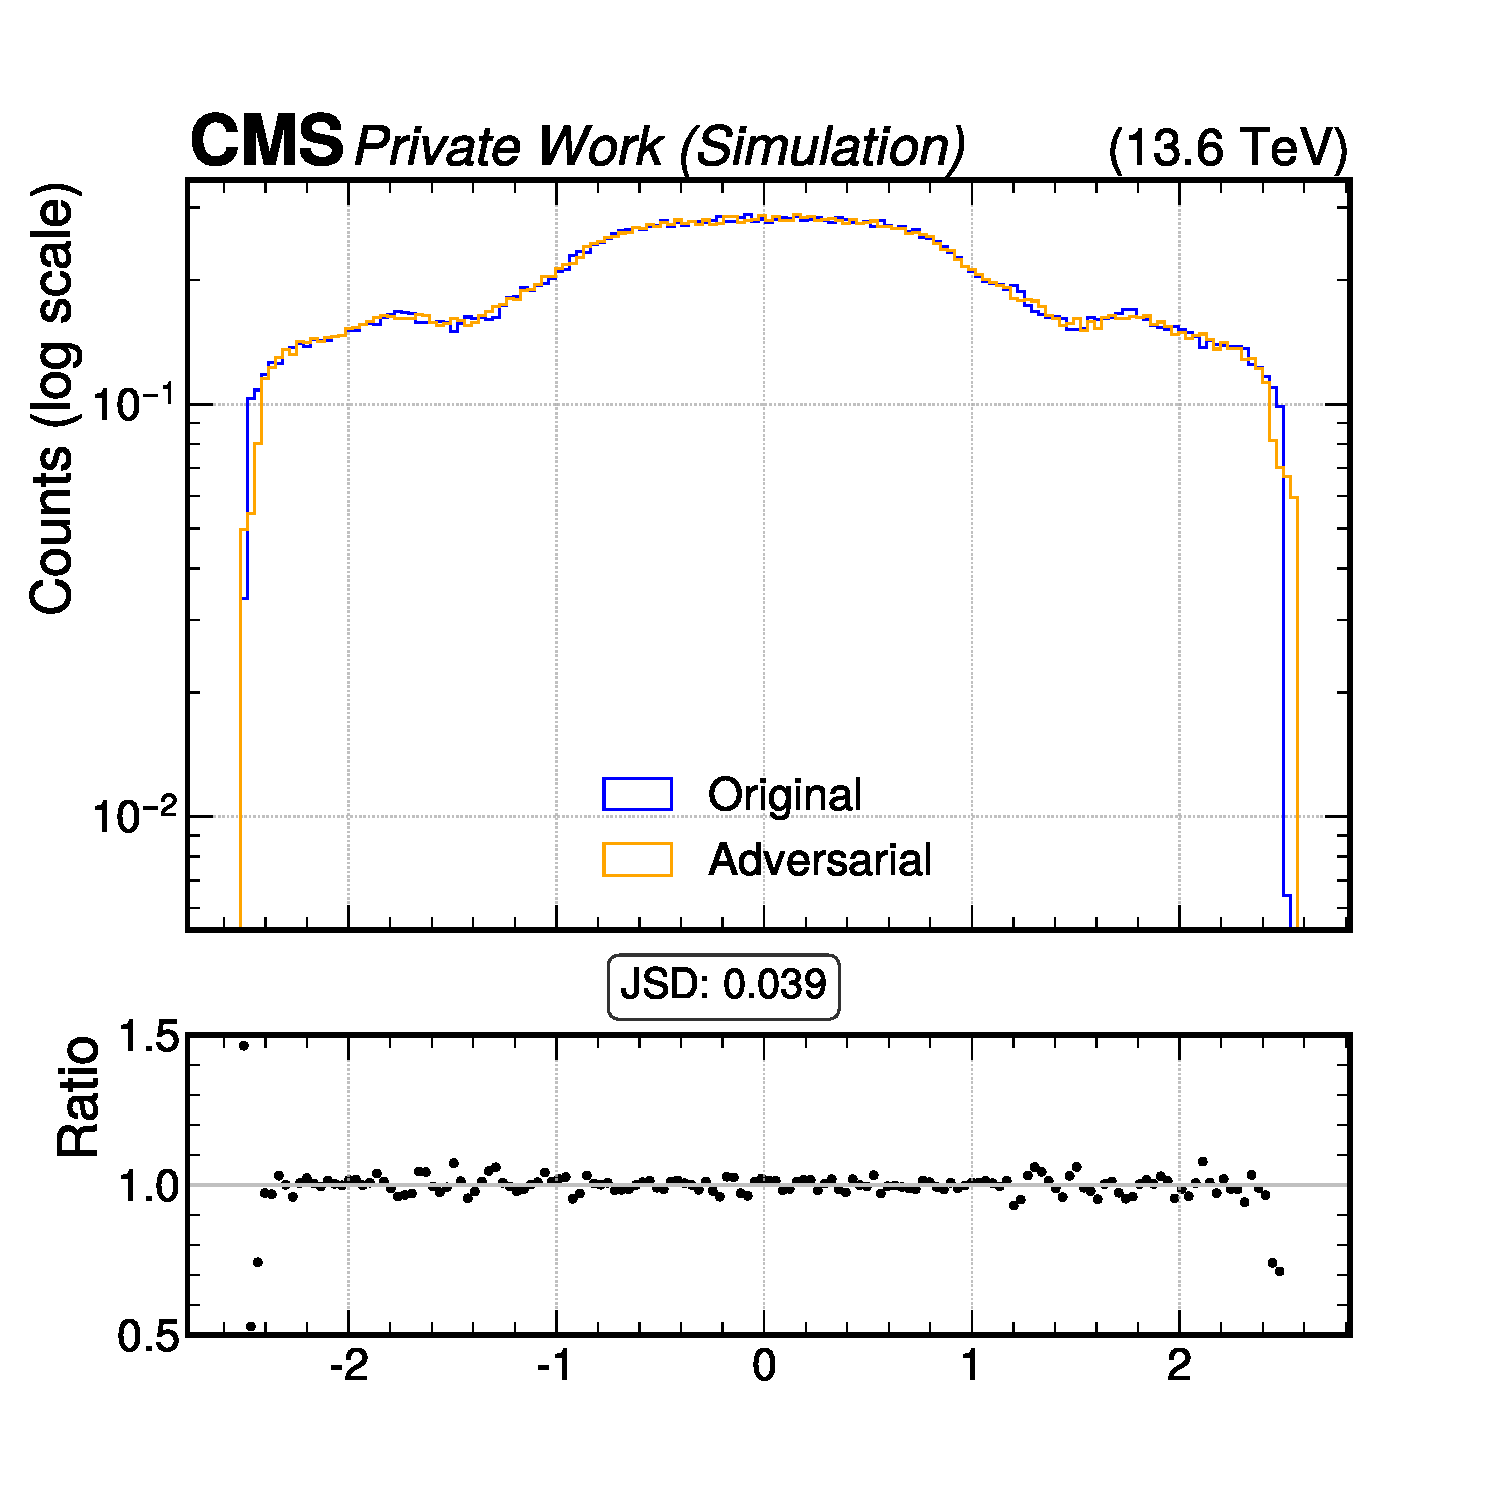
\includegraphics[width=\linewidth]{media/output/features/compare/combined_it_1/cmp_global_features_jet_eta.pdf}
    \caption{Input similarity for PIP-PGD(1).}
    \label{fig:left}
  \end{subfigure}\hfill
  \begin{subfigure}[t]{0.5\textwidth}
    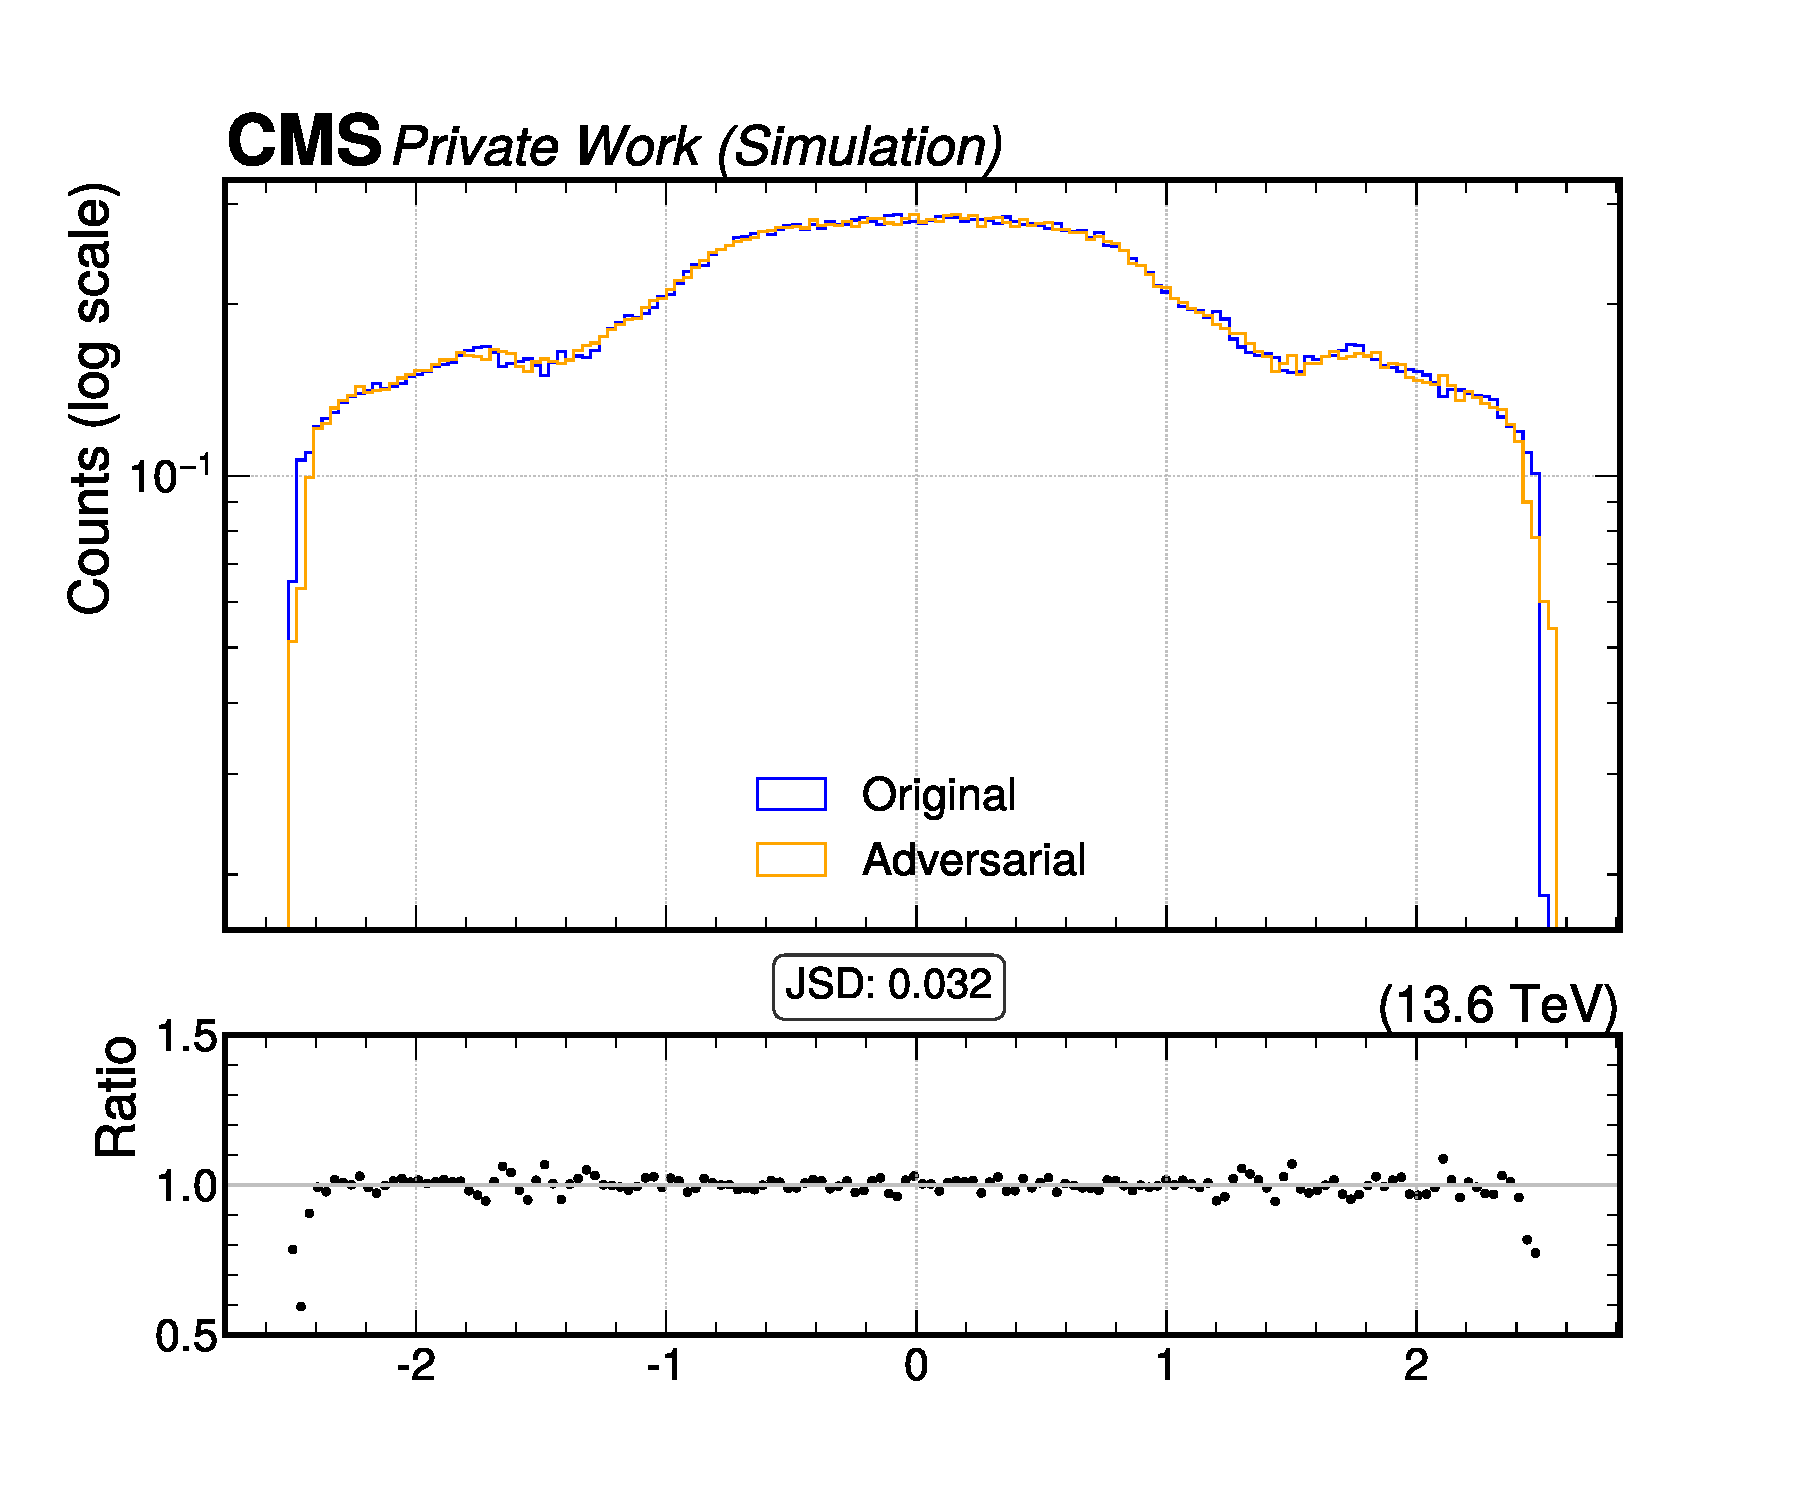
\includegraphics[width=\linewidth]{media/output/features/compare/combined_it_2/cmp_global_features_jet_eta.pdf}
    \caption{Input similarity for PIP-PGD(2).}
    \label{fig:middle}
  \end{subfigure}\hfill

  \caption{Histogram of input perturbation for continuously-valued global \texttt{jet\_eta} for one (left) and two (right) iterations of PIP-PGD compared against nominal inputs.}
  \label{fig:combined_input_eta}
\end{figure}

\begin{figure}[htbp]
  \centering
  \begin{subfigure}[t]{0.5\textwidth}
    \includegraphics[width=\linewidth]{media/output/features/compare/combined_it_1/cmp_global_features_nsv.pdf}
    \caption{Input similarity for PIP-PGD(1).}
    \label{fig:left}
  \end{subfigure}\hfill
  \begin{subfigure}[t]{0.5\textwidth}
    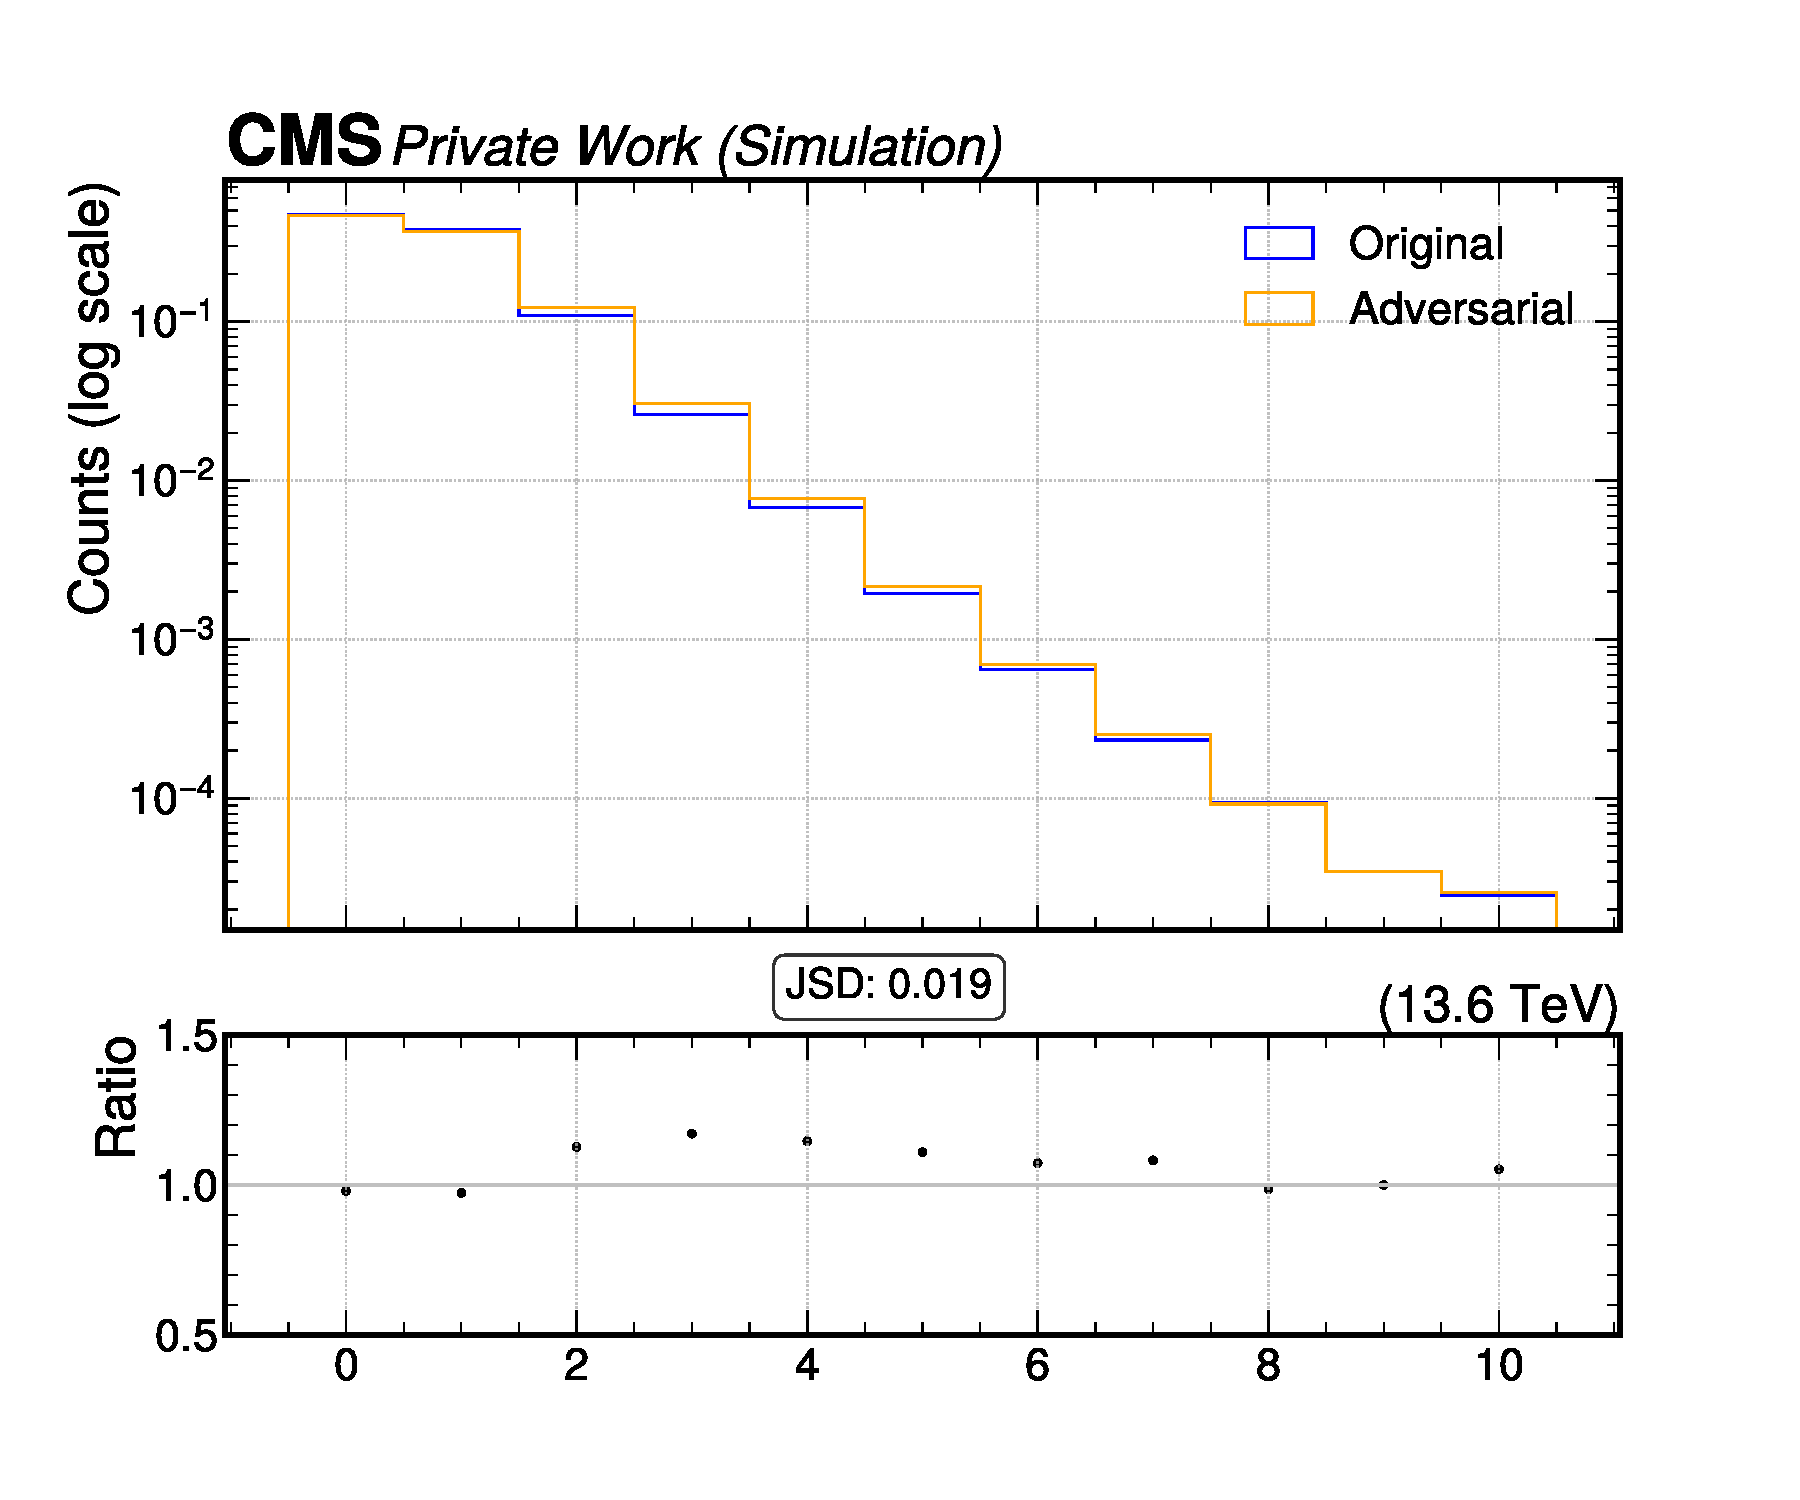
\includegraphics[width=\linewidth]{media/output/features/compare/combined_it_2/cmp_global_features_nsv.pdf}
    \caption{Input similarity for PIP-PGD(2).}
    \label{fig:middle}
  \end{subfigure}\hfill

  \caption{Histogram of input perturbation for discrete-valued global \texttt{nsv} for one (left) and two (right) iterations of PIP-PGD compared against nominal inputs.}
  \label{fig:combined_input_vtxAss}
\end{figure}

Figure \ref{fig:combined_joint_overview} provides an overview of input similarity across all features for the combined PIP-PGD attack, highlighting how different feature types respond to the hybrid perturbation strategy. While certain integer features — which are denoted orange in the figure — such as \\ \texttt{TagVarCSV\_jetNTracksEtaRel}, \texttt{TagVarCSV\_vertexCategory} or \texttt{Cpfcan\_quality} exhibit larger perturbations than others, their overall similarity remains comparable.


\begin{figure}[H]
\centering
    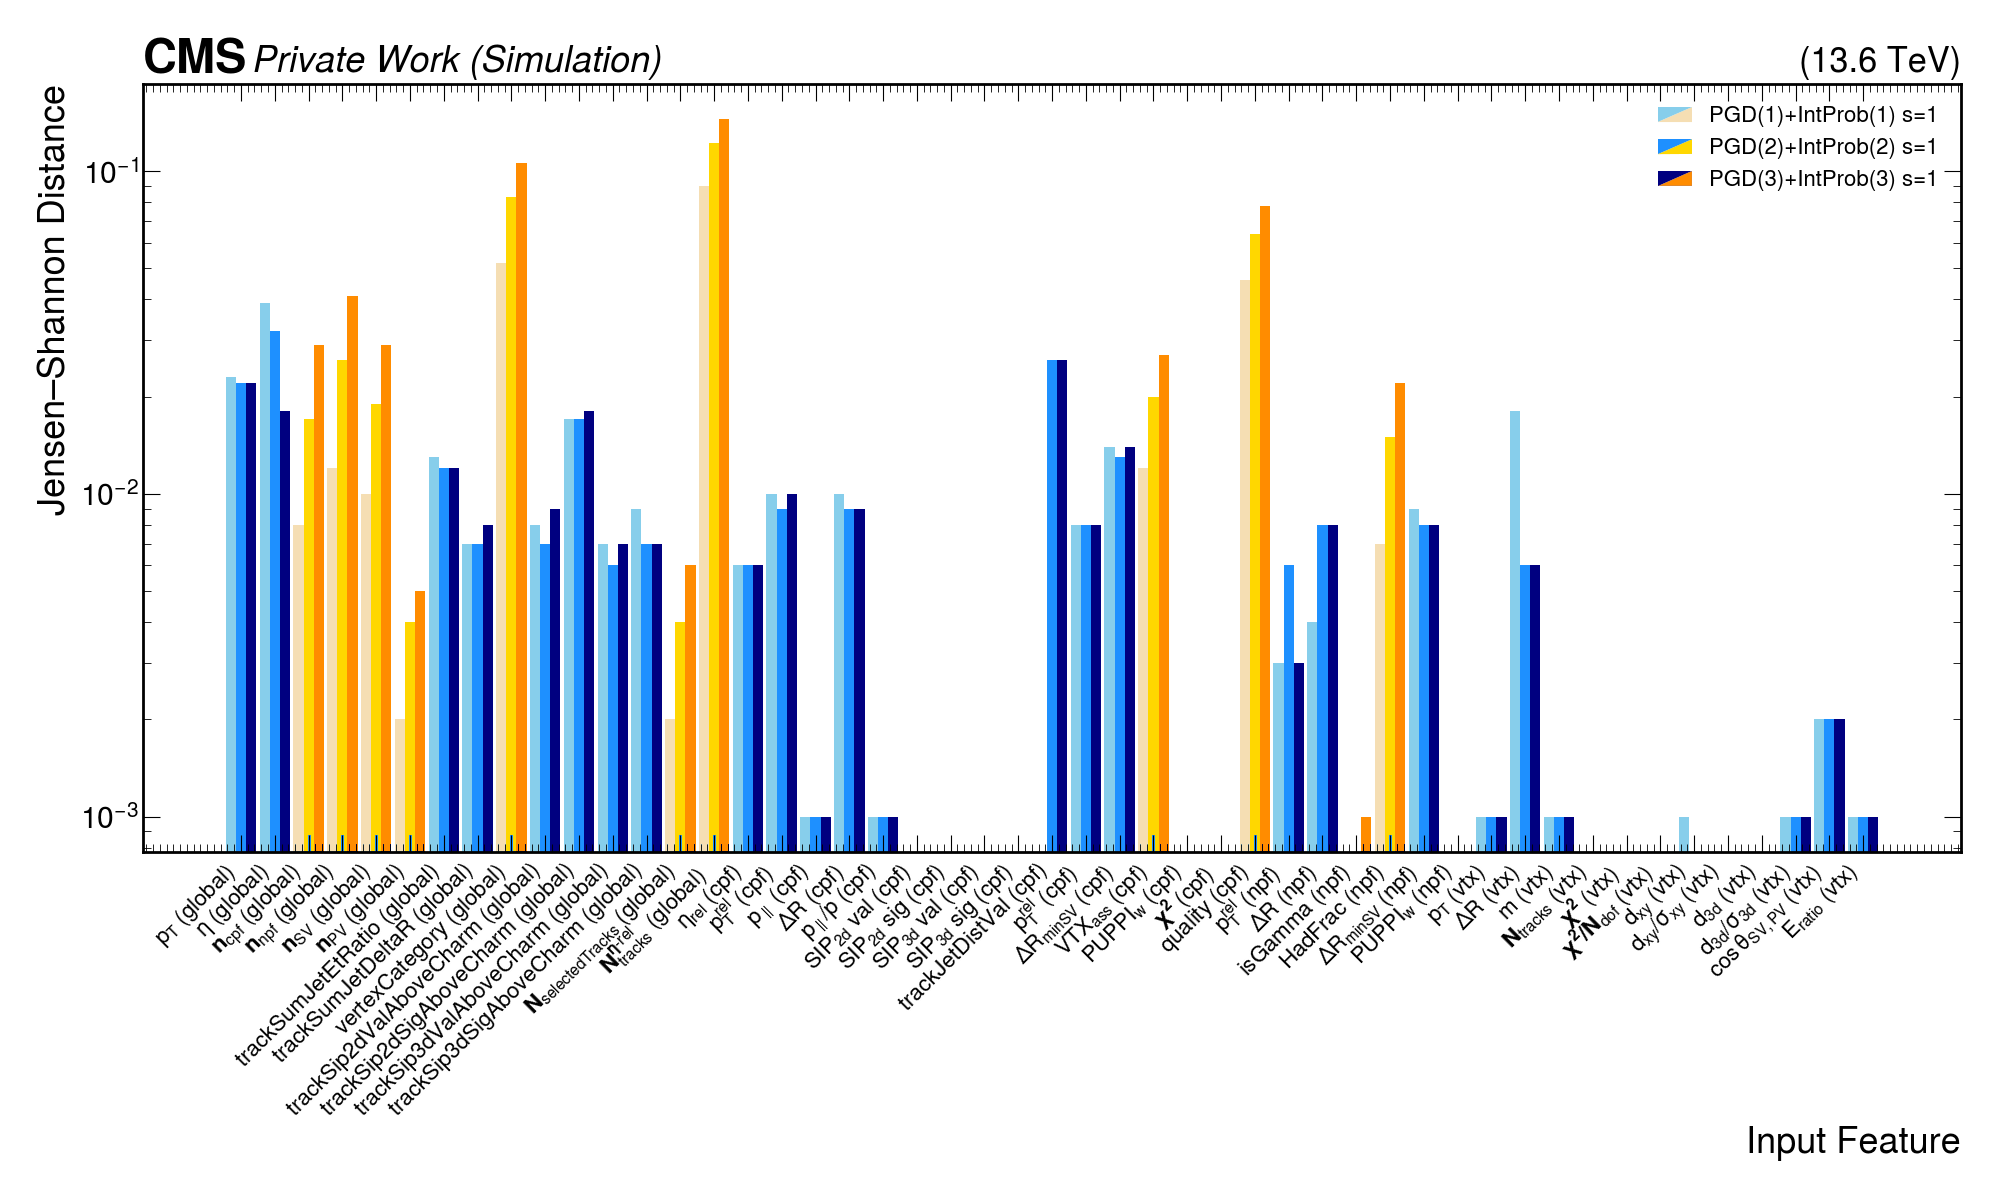
\includegraphics[width=15cm]{media/output/features/compare/jsd_comb_per_feature.pdf}
    \caption{JSD input similarity development for different iterations of the PIP-PGD attack for $s=1$ and $\epsilon=0.1$ while attributing for individual features. Orange bars denote integer based features, blue bars correspond to floating-point features. Values below $10^{-1}$ are not included due to rounding.}
    \label{fig:combined_joint_overview}
\end{figure}

The pattern indicates that the combined attack balances stealth and efficacy effectively: integer features introduce targeted modifications atop continuous feature perturbations, enabling a more aggressive perturbation strategy. 

\paragraph{Attack:} This increased aggression is apparent for variations in the applied sharpness ranging from a slight degradation at $s=5$ ($AUC=0.936$) towards a moderate impact at $s=1$ ($AUC=0.928$) and a severe degradation at $s=0.5$ with an AUC of $0.916$  as seen in figure \ref{fig:combined_testing_sharpness}. The gap between nominal performance ($AUC=0.965$) and PIP at $s=5$ is predominately caused by PGD(1) ($AUC=0.937$, see figure \ref{fig:pgd_trained}).

\begin{figure}[h]
\centering
    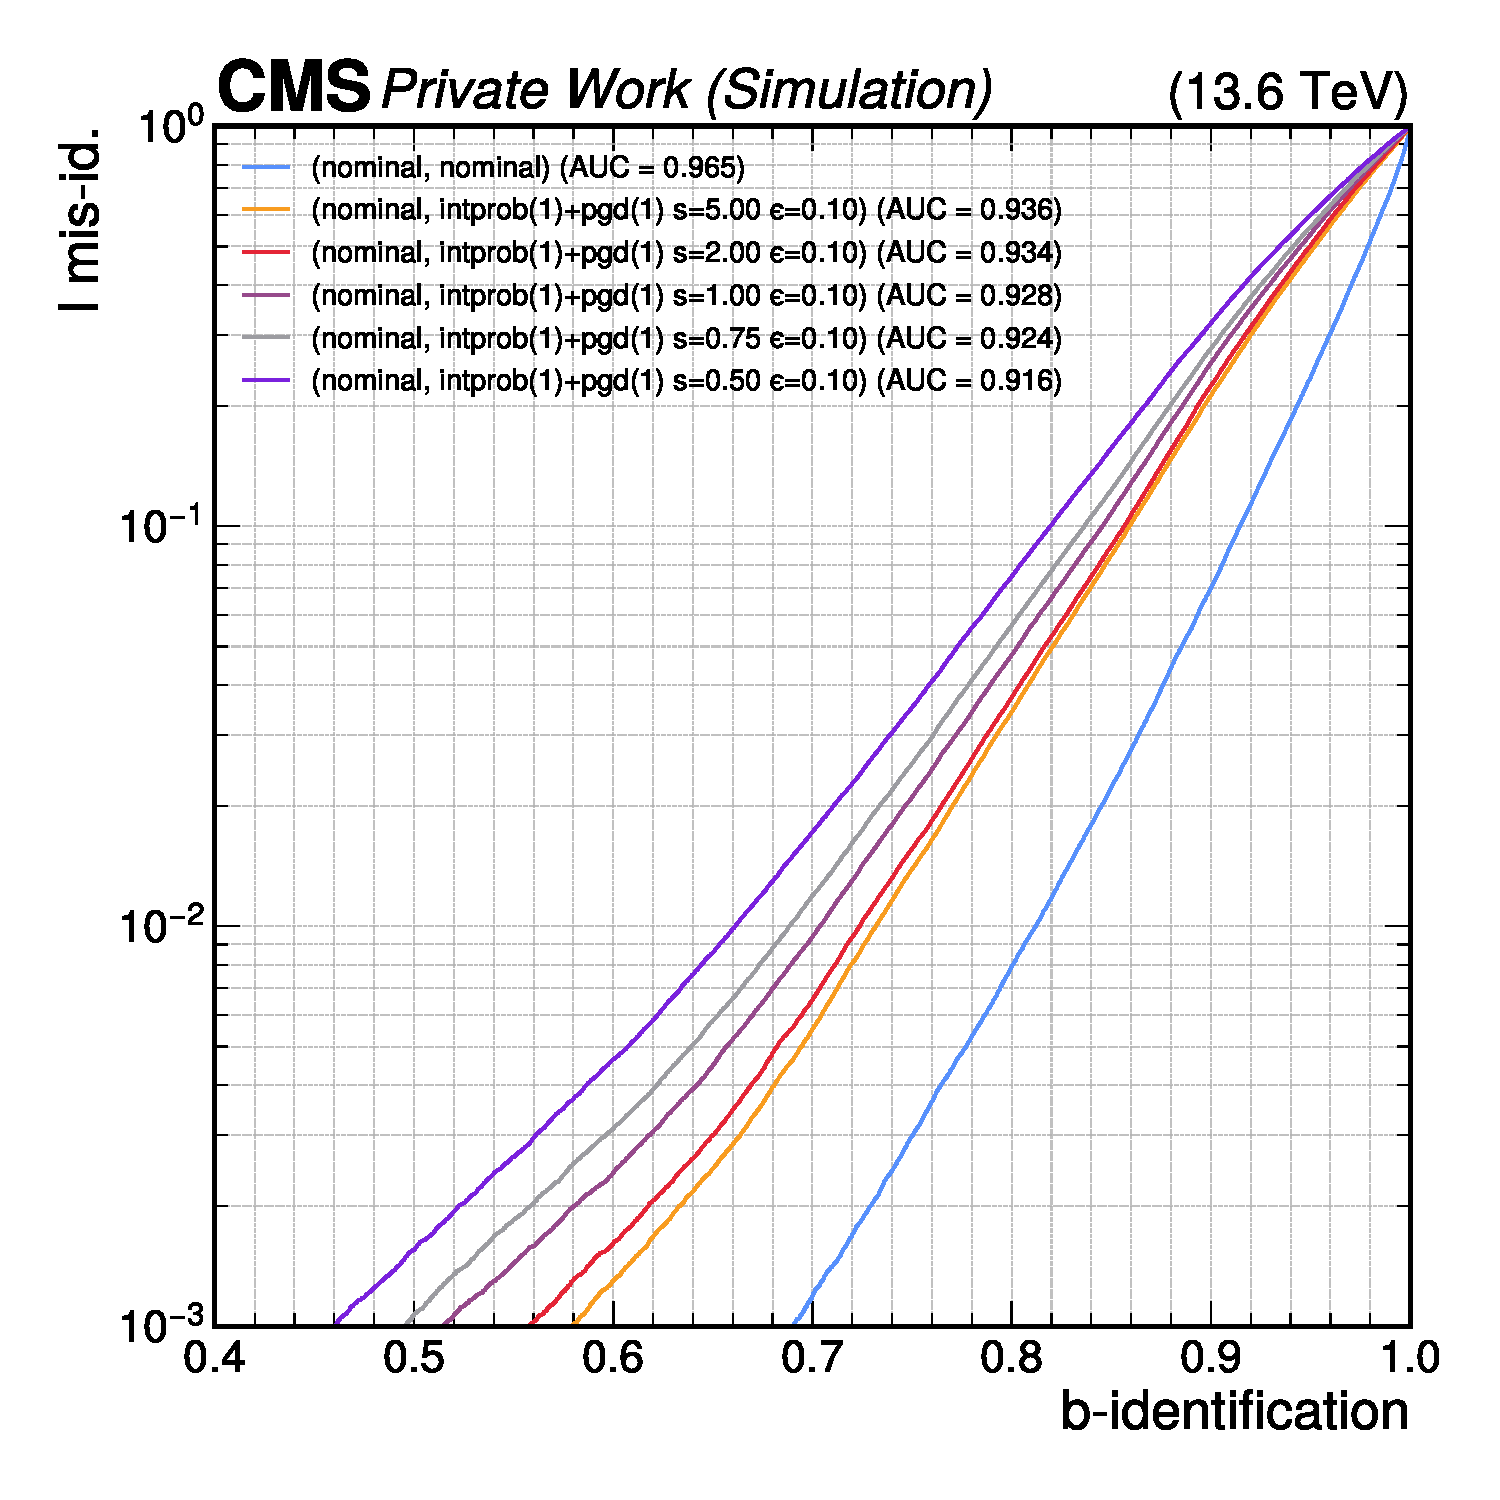
\includegraphics[width=15cm]{media/output/roc_bvsl_combined_sharpness.pdf}
    \caption{AUC score of BvsL misidentification for PIP-PGD with sharpness between $s=0.5$ and $s=5$ at one iteration with a magnitude of $\epsilon=0.10$ tested against the nominal trained model.}
    \label{fig:combined_testing_sharpness}
\end{figure}

Likewise, the AUC score degrades with increasing iterations for the combined PIP-PGD attack from $AUC=0.928$ at one iteration towards stark inference of $AUC=0.885$ at five (see figure \ref{fig:combined_testing_iterations}). The continued AUC decline for iterations > 1 is largely due to PIP stochastic nature, as discussed in Section \ref{sec:inprob_result}.

\begin{figure}[h]
\centering
    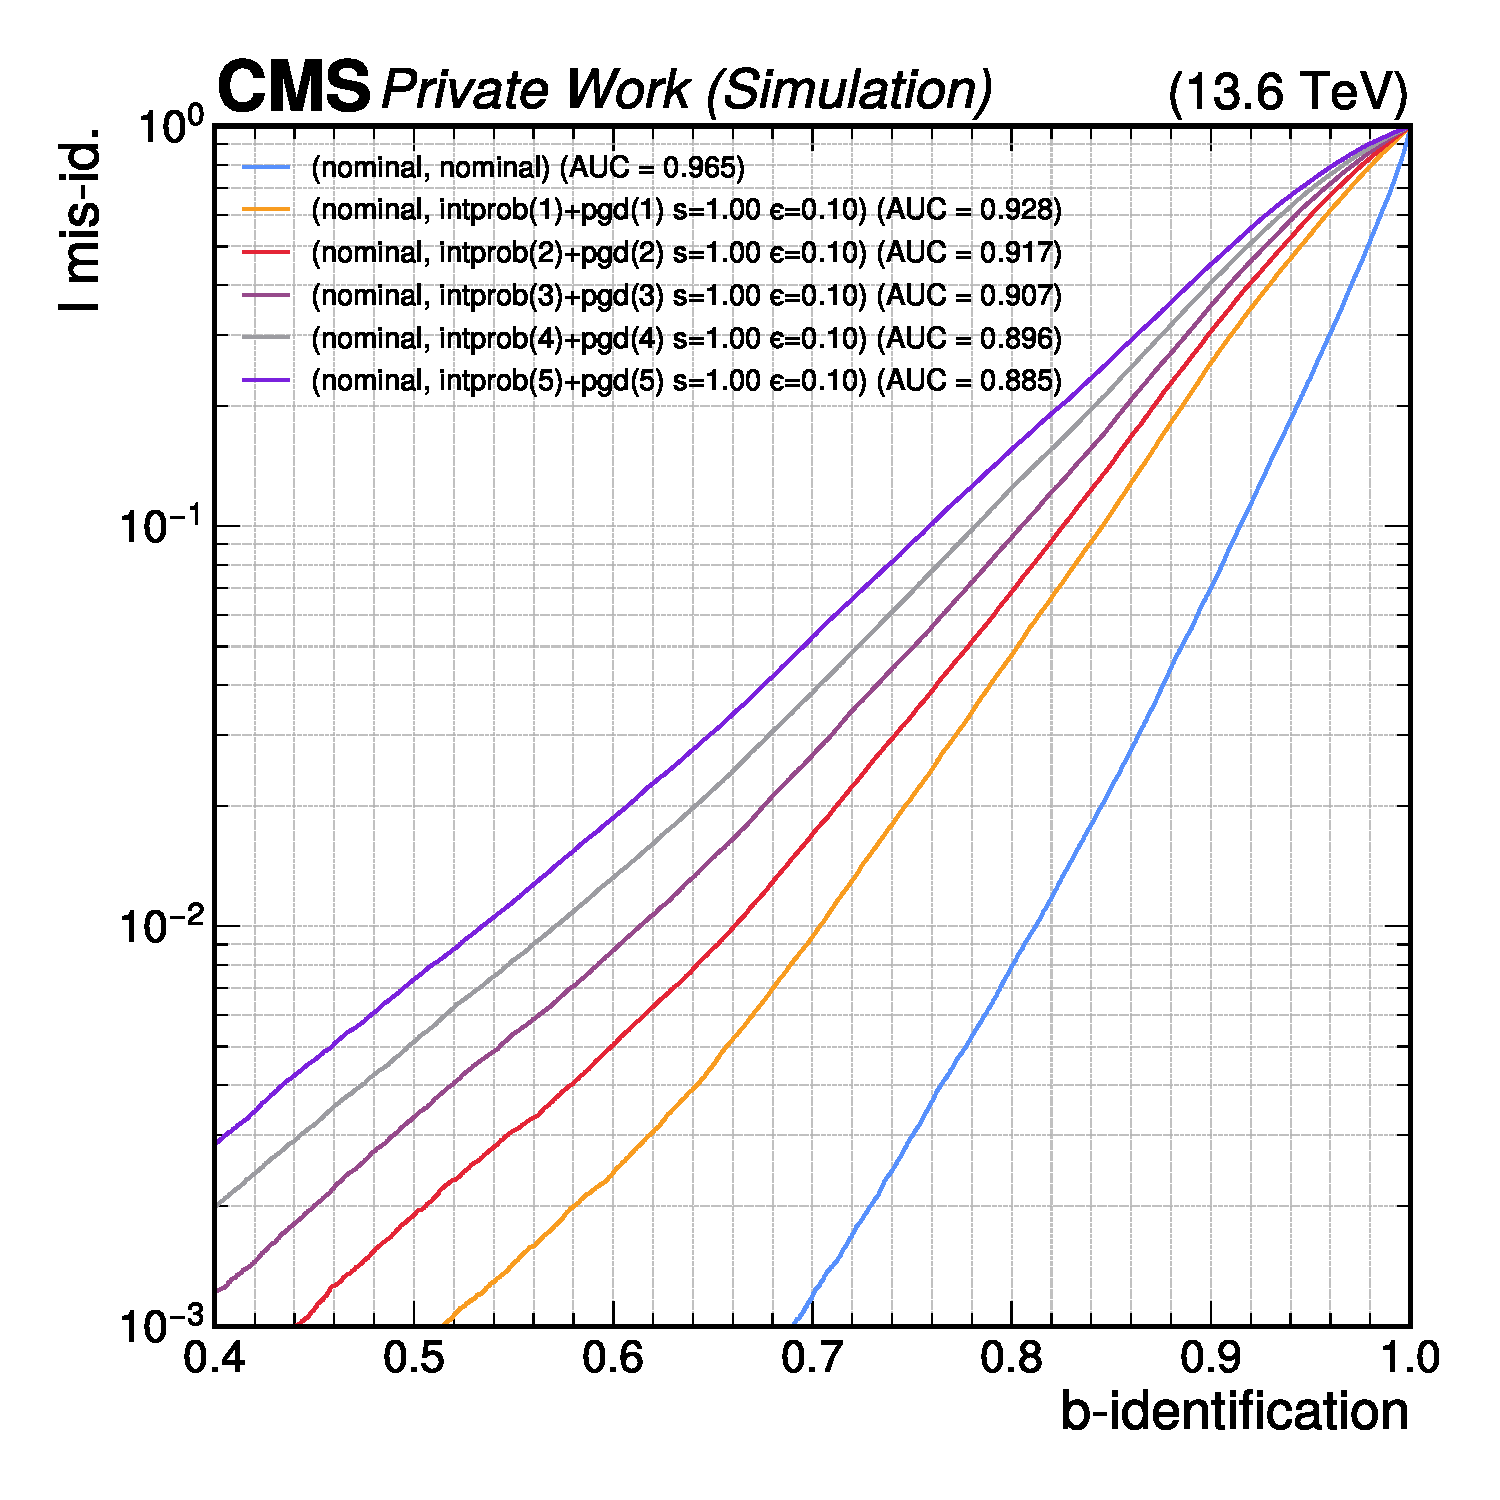
\includegraphics[width=15cm]{media/output/roc_bvsl_combined_iterations.pdf}
    \caption{AUC score of PIP-PGD for BvsL misidentification for up to 5 iterations with a fixed magnitude of $\epsilon=0.1$ and a sharpness of $s=1$ tested against the nominal trained model.}
    \label{fig:combined_testing_iterations}
\end{figure}


\begin{figure}[H]
\centering
    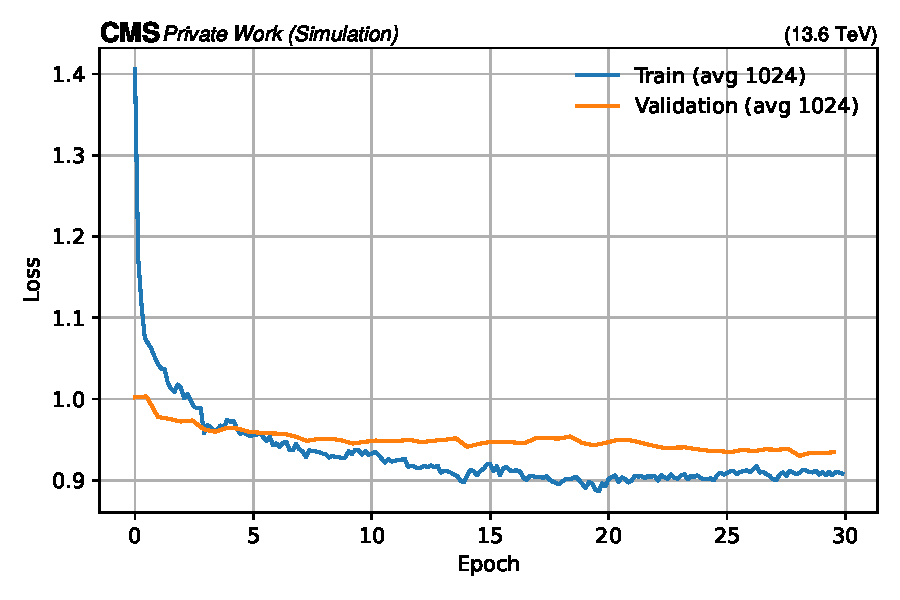
\includegraphics[width=15cm]{media/output/combined_loss_validation.pdf}
    \caption{Training and validation loss for PIP-PGD(1) with a sharpness of $s=1$ and a magnitude of $\epsilon=0.1$, while scaling individual attack features based on an epsilon tensor.}
    \label{fig:combined_training_loss}
\end{figure}


\FloatBarrier
\paragraph{Adversarial Training:} The training loss curve (see figure \ref{fig:combined_training_loss}) for PIP-PGD exhibits moderate volatility, falling between the stability of pure PGD training and the higher volatility of PIP training . This intermediate behaviour is attributable to the model's need to develop defences that are effective against continuous and probabilistic discrete modifications.



The validation loss demonstrates robust generalization, suggesting that the combined training approach successfully teaches the model to recognize and resist both perturbation types. The convergence pattern indicates that the model learns to balance the competing objectives of maintaining nominal performance while developing comprehensive adversarial defences.

Notably, the final validation loss values are competitive with single-method adversarial training and even surpass pure PIP training. This is an indication that the combined approach does not sacrifice overall performance for broader robustness. It furthermore suggests that the two perturbation types target complementary aspects of the model's decision boundaries, allowing for more comprehensive defence development.

The training efficiency appears reasonable, with convergence achieved within a similar time frame to single-method approaches. This efficiency is particularly important given the increased computational complexity of generating both types of adversarial examples during training.

\begin{figure}[h]
\centering
    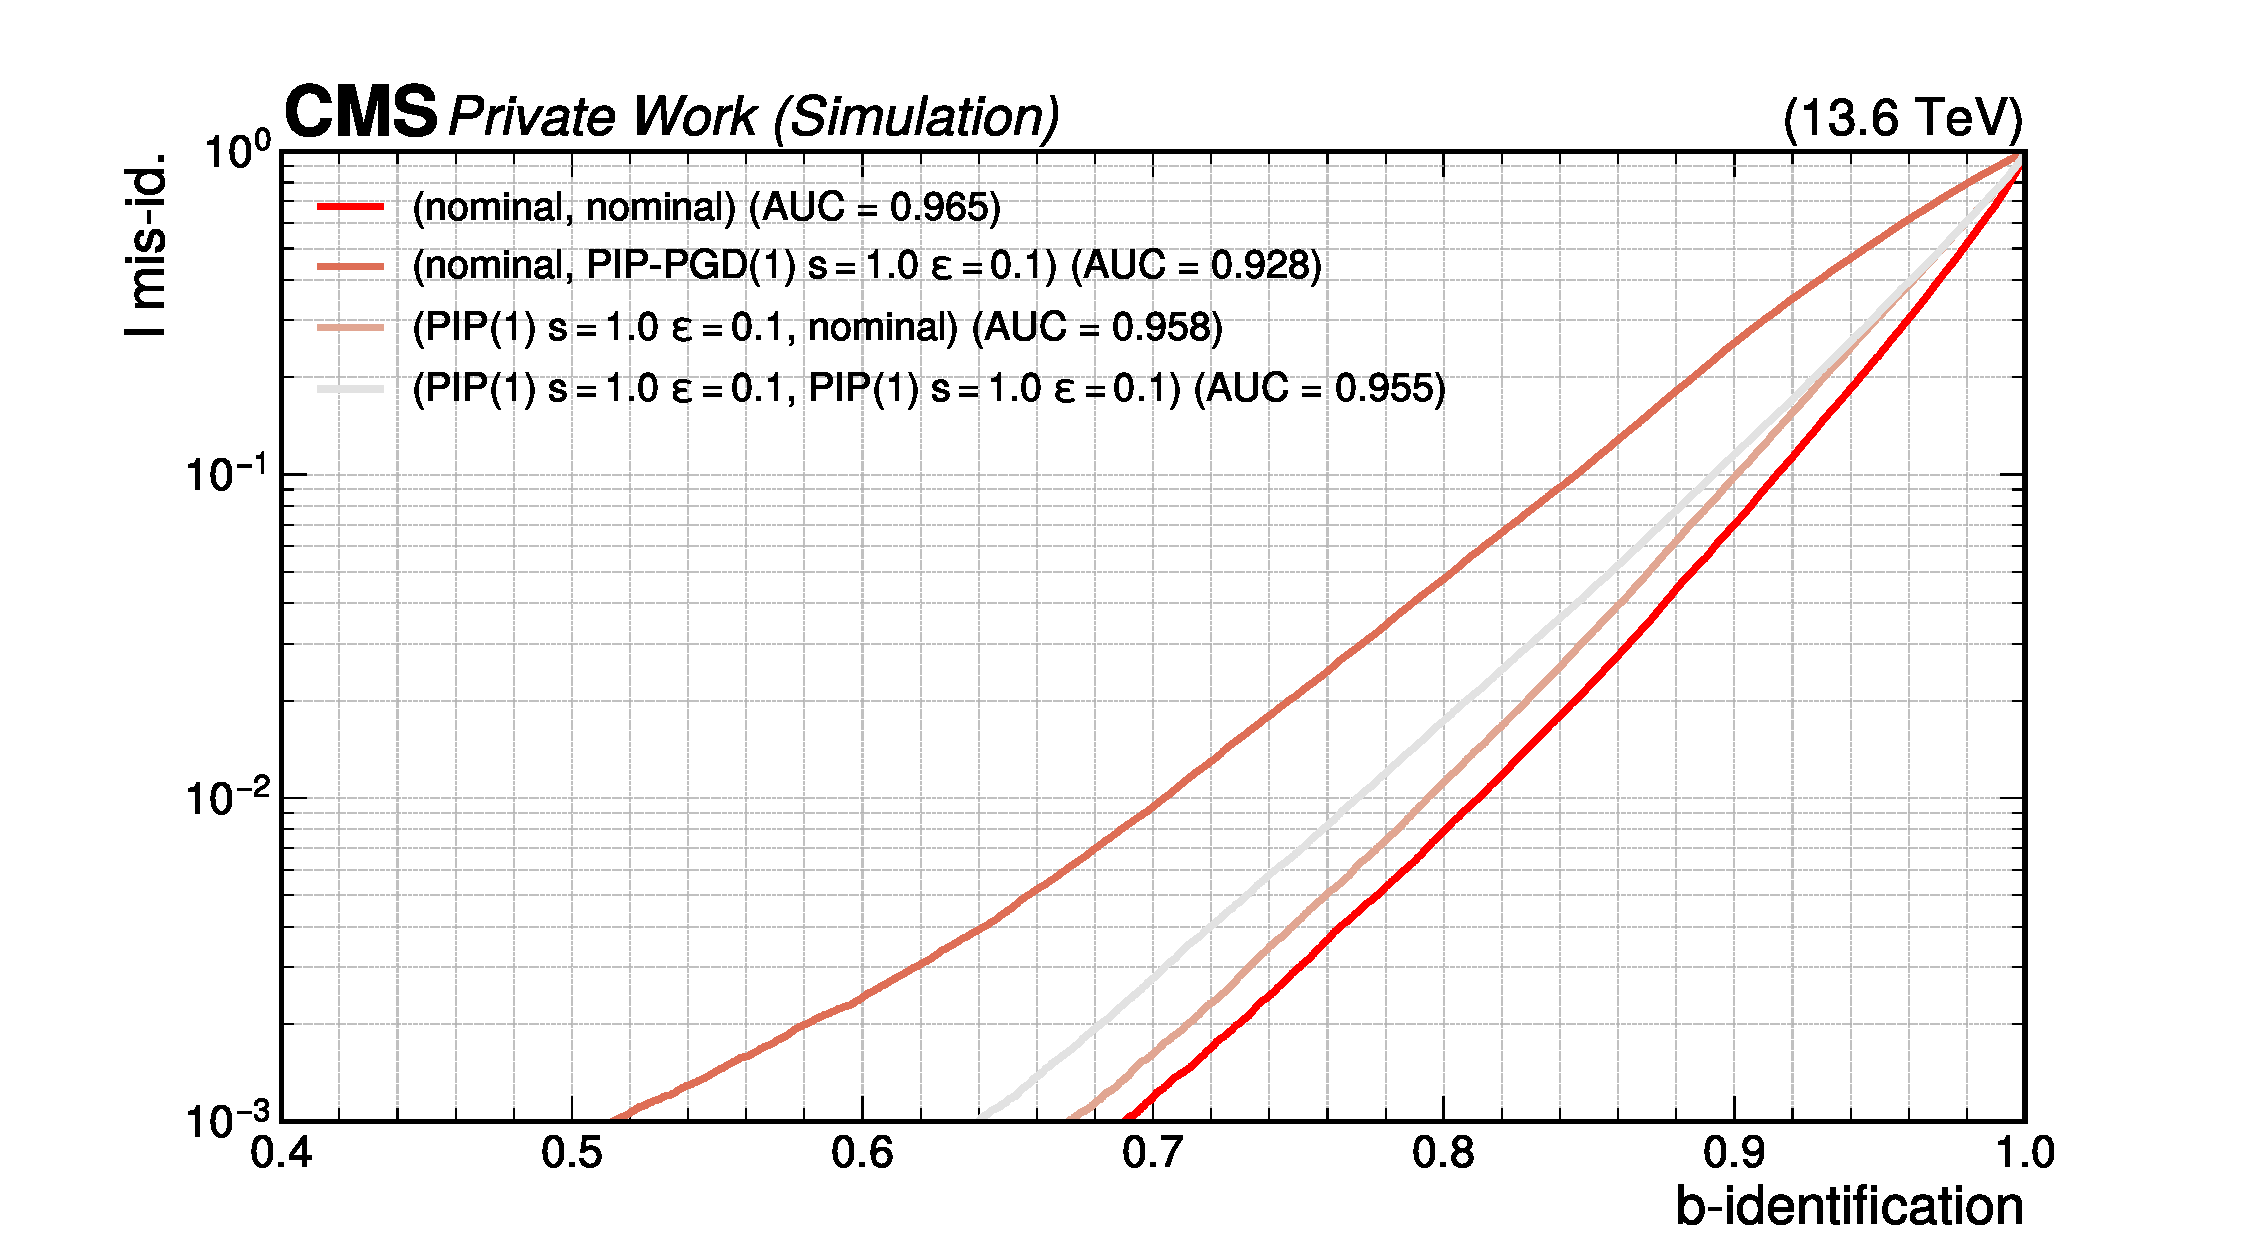
\includegraphics[width=15cm]{media/output/roc_bvsl_combined_crossing.pdf}
    \caption{ROC curves for BvsL misidentification for a PIP-PGD(1) and nominal trained model tested against nominal or PIP-PGD(1) perturbed inputs with $s=1.0$ and $\epsilon=0.1$.}
    \label{fig:joint_training_crossing}
\end{figure}

Figure \ref{fig:joint_training_crossing} shows that the adversarially trained PIP-PGD model, with an AUC of $0.958$ against nominal inputs, closely matches the baseline AUC for nominal inputs ($AUC = 0.965$). It also demonstrates robustness across PGD ($AUC = 0.952$), PIP ($AUC = 0.960$), and itself ($AUC = 0.955$). Compared to the nominal-trained model on PIP-PGD perturbed data ($AUC = 0.928$), the PIP-PGD model achieves consistently strong performance across all tested scenarios.




\FloatBarrier
\section{Transferability and Cross-Robustness}

This section concludes the evaluation of PIP by assessing the transferability and cross-robustness of adversarial training strategies, with a focus on the combined PIP-PGD attack. By analysing the interplay of \textit{iteration count} and \textit{sharpness} in PIP’s variability and assessing robustness across diverse attack scenarios, it is demonstrated how the hybrid approach balances efficacy and generalization.

\subsection{Variability of PIP}
\label{sec:intprob_variability}

\begin{figure}[h]
\centering
    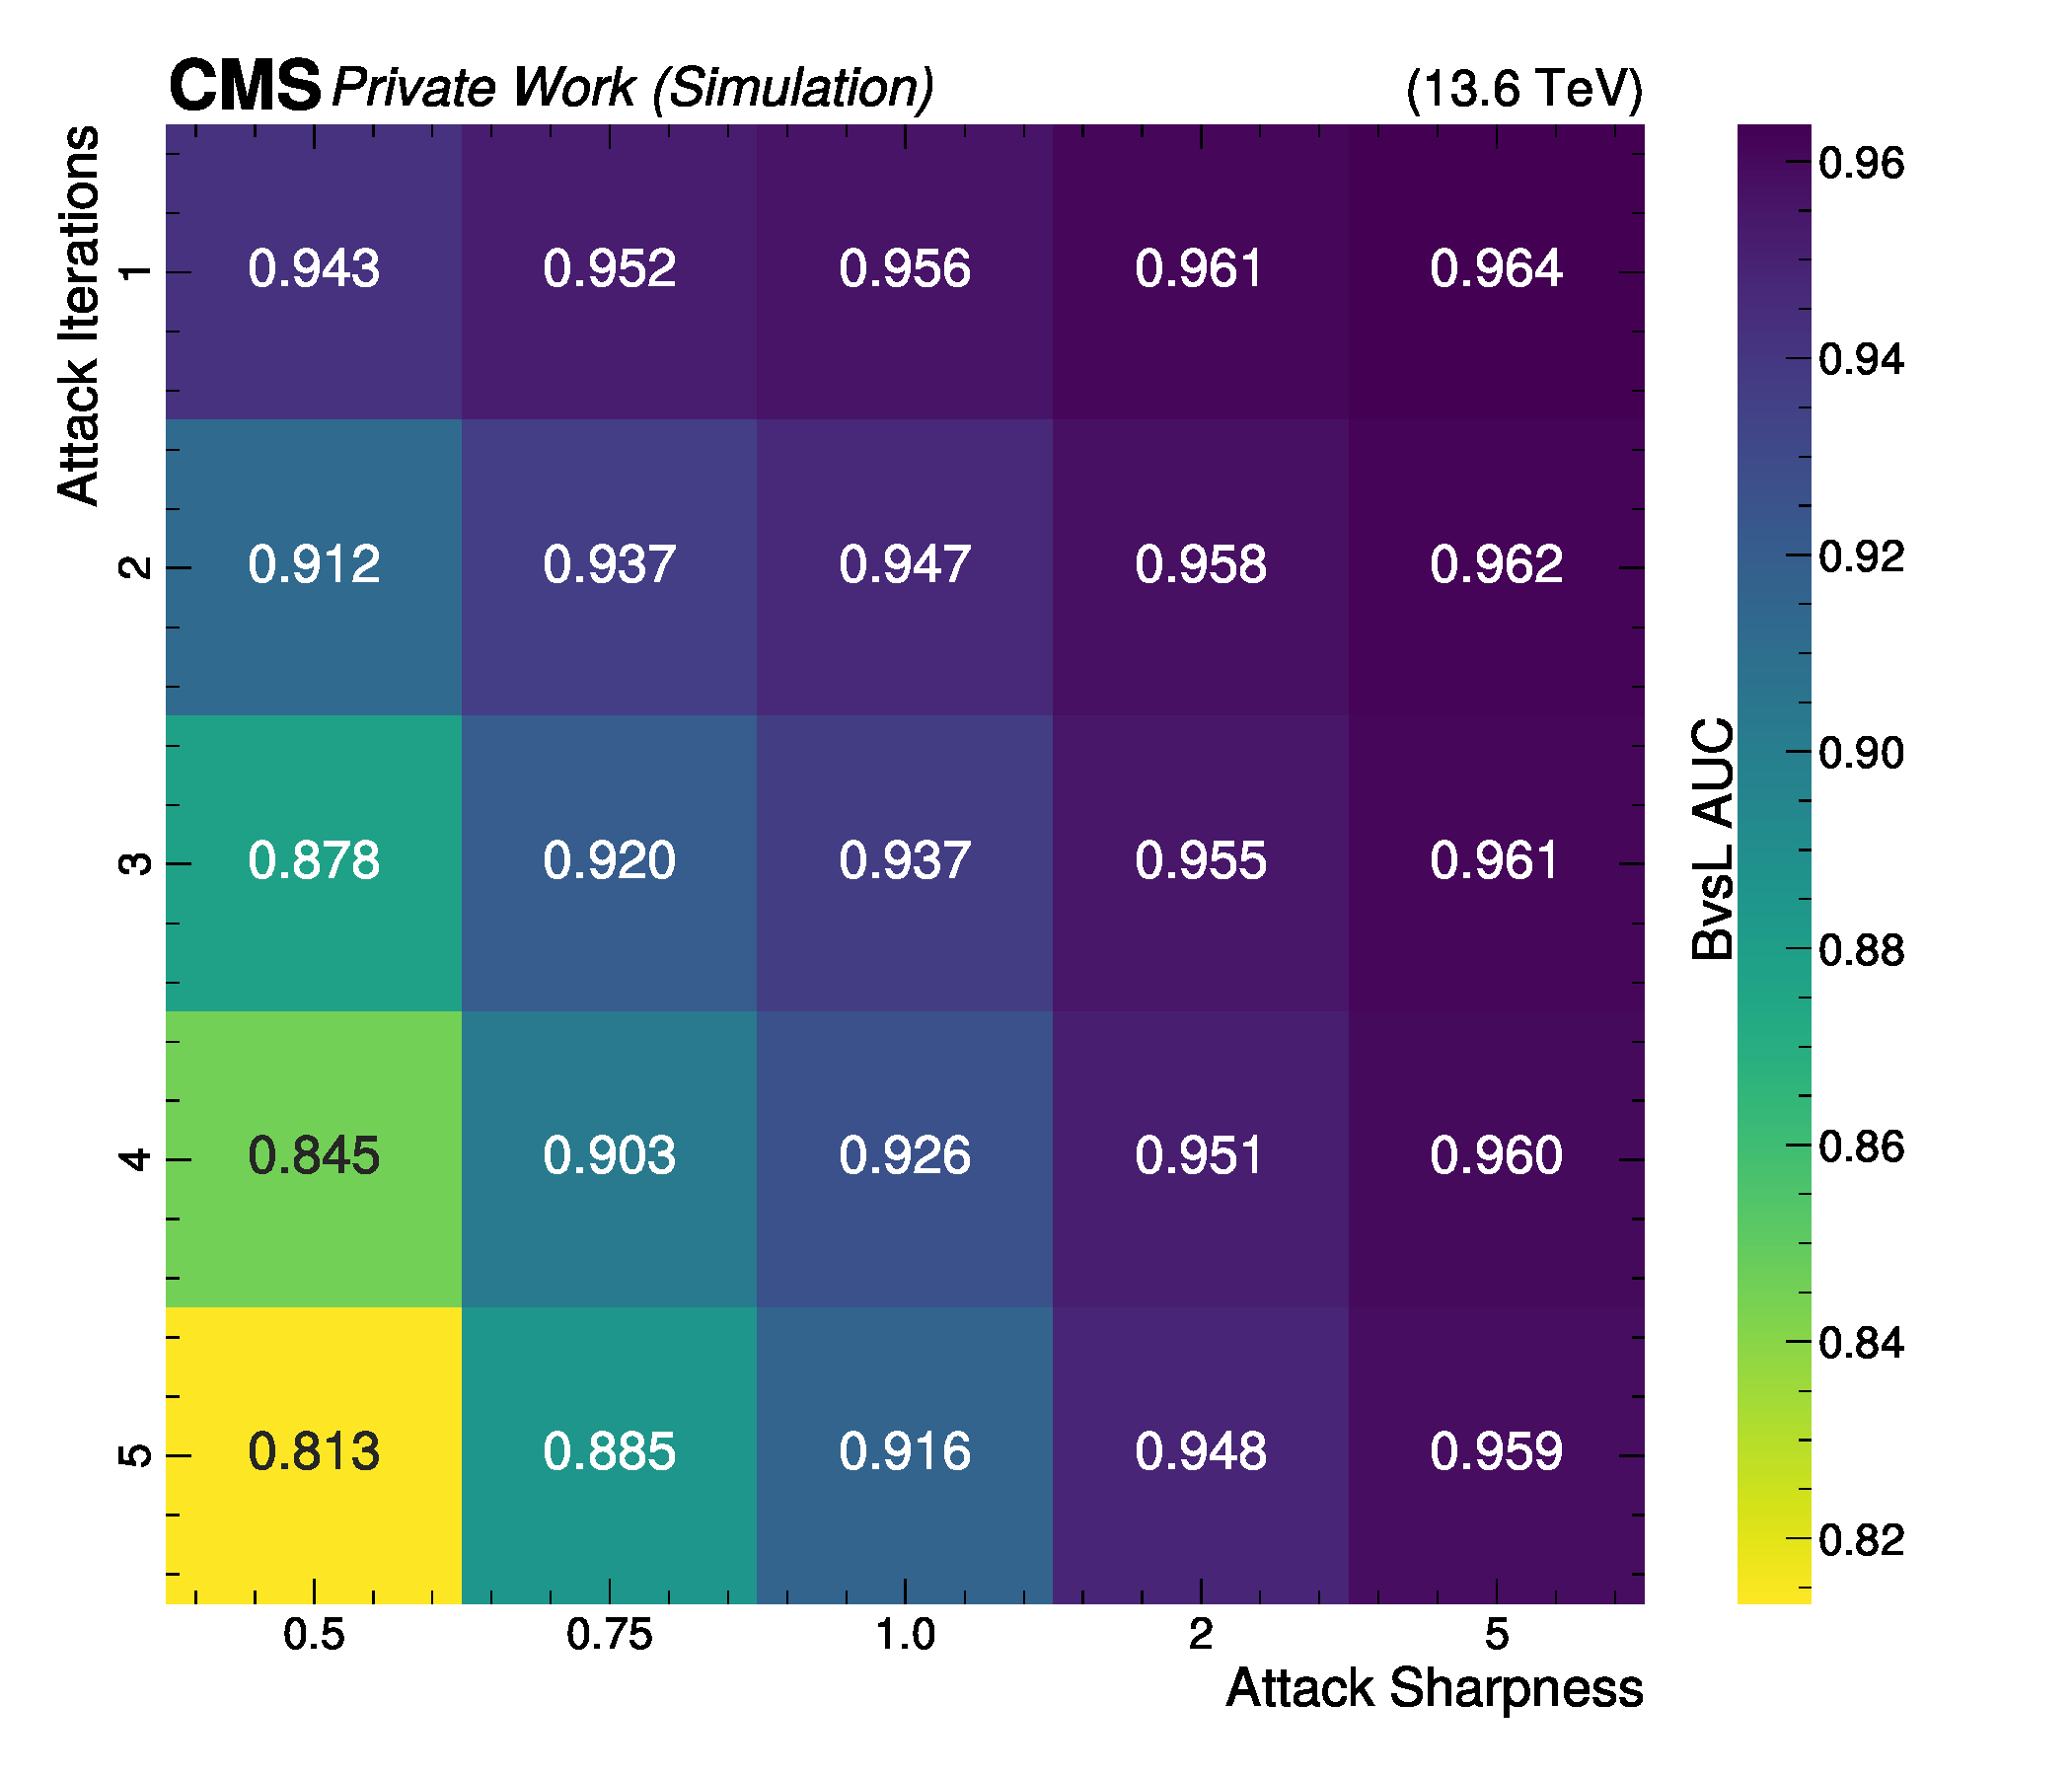
\includegraphics[width=15cm]{media/output/sharpness_iterations_scan.pdf}
    \caption{AUC score matrix of BvsL misidentification for different iteration and sharpness values in the PIP-PGD attack tested against the nominal trained model.}
    \label{fig:joint_sharpness_vs_iterarions}
\end{figure}

Figure~\ref{fig:joint_sharpness_vs_iterarions} visualises the impact of jointly varying the \emph{iteration count} $k$ (rows) and the \emph{sharpness} parameter $s$ (columns) on the attack efficacy for PIP. For each $(k,s)$ point the resulting BvsL AUC is reported after the attack has been applied to the nominally trained model. Notably, the heatmap is inverted to emphasize stronger degradation from the nominal baseline.

\newpage
\paragraph{Key trends.}
\begin{enumerate}
  \item \textbf{Iteration depth controls raw attack power.}  
        Increasing from $k=1$ (single-step FGSM/PIP) to $k=5$ the AUC degrades monotonically, with the most pronounced drop occurring for low-$s$ columns.  Concretely, the AUC falls from $0.943$ to $0.813$ at
        $(s{=}0.5)$ — a relative reduction of roughly 13\% for only four extra gradient evaluations.
  \item \textbf{Sharpness $s$ trades off focus against coverage.}
        As anticipated in section \ref{sec:intprob_methodology}, large $s$ produces a more sparse integer perturbation pattern, meaning the attack relies mainly on the continuous PGD component. This yields noticeably smaller AUC drops (right-most column remains ${\gtrsim}0.959$ even at $k{=}5$).
        Conversely, $s\!\le\!1$ flips a broader set of integer features; the
        attack strength then scales almost linearly with $k$.
  \item \textbf{Region for practical settings.}  
        The contour where $\text{AUC}\!\approx\!0.937$ — the same degradation as for PGD(1) — occurs at $(k{=}3,\,s{=}1)$. Any application of a combined attack should therefore lie below this threshold (so at higher sharpness or less iterations) to not overshadow the application of PGD(1).
\end{enumerate}

The heatmap highlights the flexibility of PIP: by adjusting iteration count $k$ and sharpness $s$, one can interpolate between subtle, nearly imperceptible perturbations and aggressive attacks that reduce the tagger’s performance by $\gtrsim15\%$, targeting only integer features. The $(k,s)$ plane is non-degenerate, with no single optimal setting; the ideal configuration depends on prioritizing stealth (larger $s$, smaller $k$) or maximum performance degradation (smaller $s$, larger $k$). Thus, PIP can be tuned to remain subtle when combined with other attacks while enhancing robustness against integer-based corruption, extending existing adversarial algorithms.

\subsection{Cross-Robustness of PIP-PGD}

The last section of this thesis focuses on a cross-robustness study between trained and tested models across all previous mentioned adversarial attacks. For the sake of simplicity, a sharpness of $s=1$, PGD magnitude of $\epsilon=0.1$, and only one iteration is discussed here.

Figure \ref{fig:cross_robustness} illustrates a key property of adversarial training with integer-based attacks. The model trained on PIP achieves excellent performance against the same attack ($AUC = 0.967$), slightly outperforming the nominal model on unperturbed data ($AUC = 0.965$). This suggests strong adaptation to the characteristic perturbations of probabilistic integer modifications. However, this enhanced robustness is highly specific to the trained attack pattern. When evaluated against other attacks, such as PGD or PIP-PGD, performance degrades noticeably, indicating a form of adversarial overfitting where the model resists a narrow class of perturbations but struggles to generalize.

In contrast, adversarial training with the PIP-PGD strategy yields more balanced robustness across all tested attack scenarios. Although its AUC on the PIP attack is slightly lower than that of models trained solely on PIP or PGD, the combined model exhibits better transferability, maintaining robust performance under both PIP ($AUC = 0.960$) and PGD ($AUC = 0.952$) attacks. This suggests that combined adversarial training mitigates attack-specific overfitting, fostering a more generalizable defence.

\begin{figure}[h]
\centering
    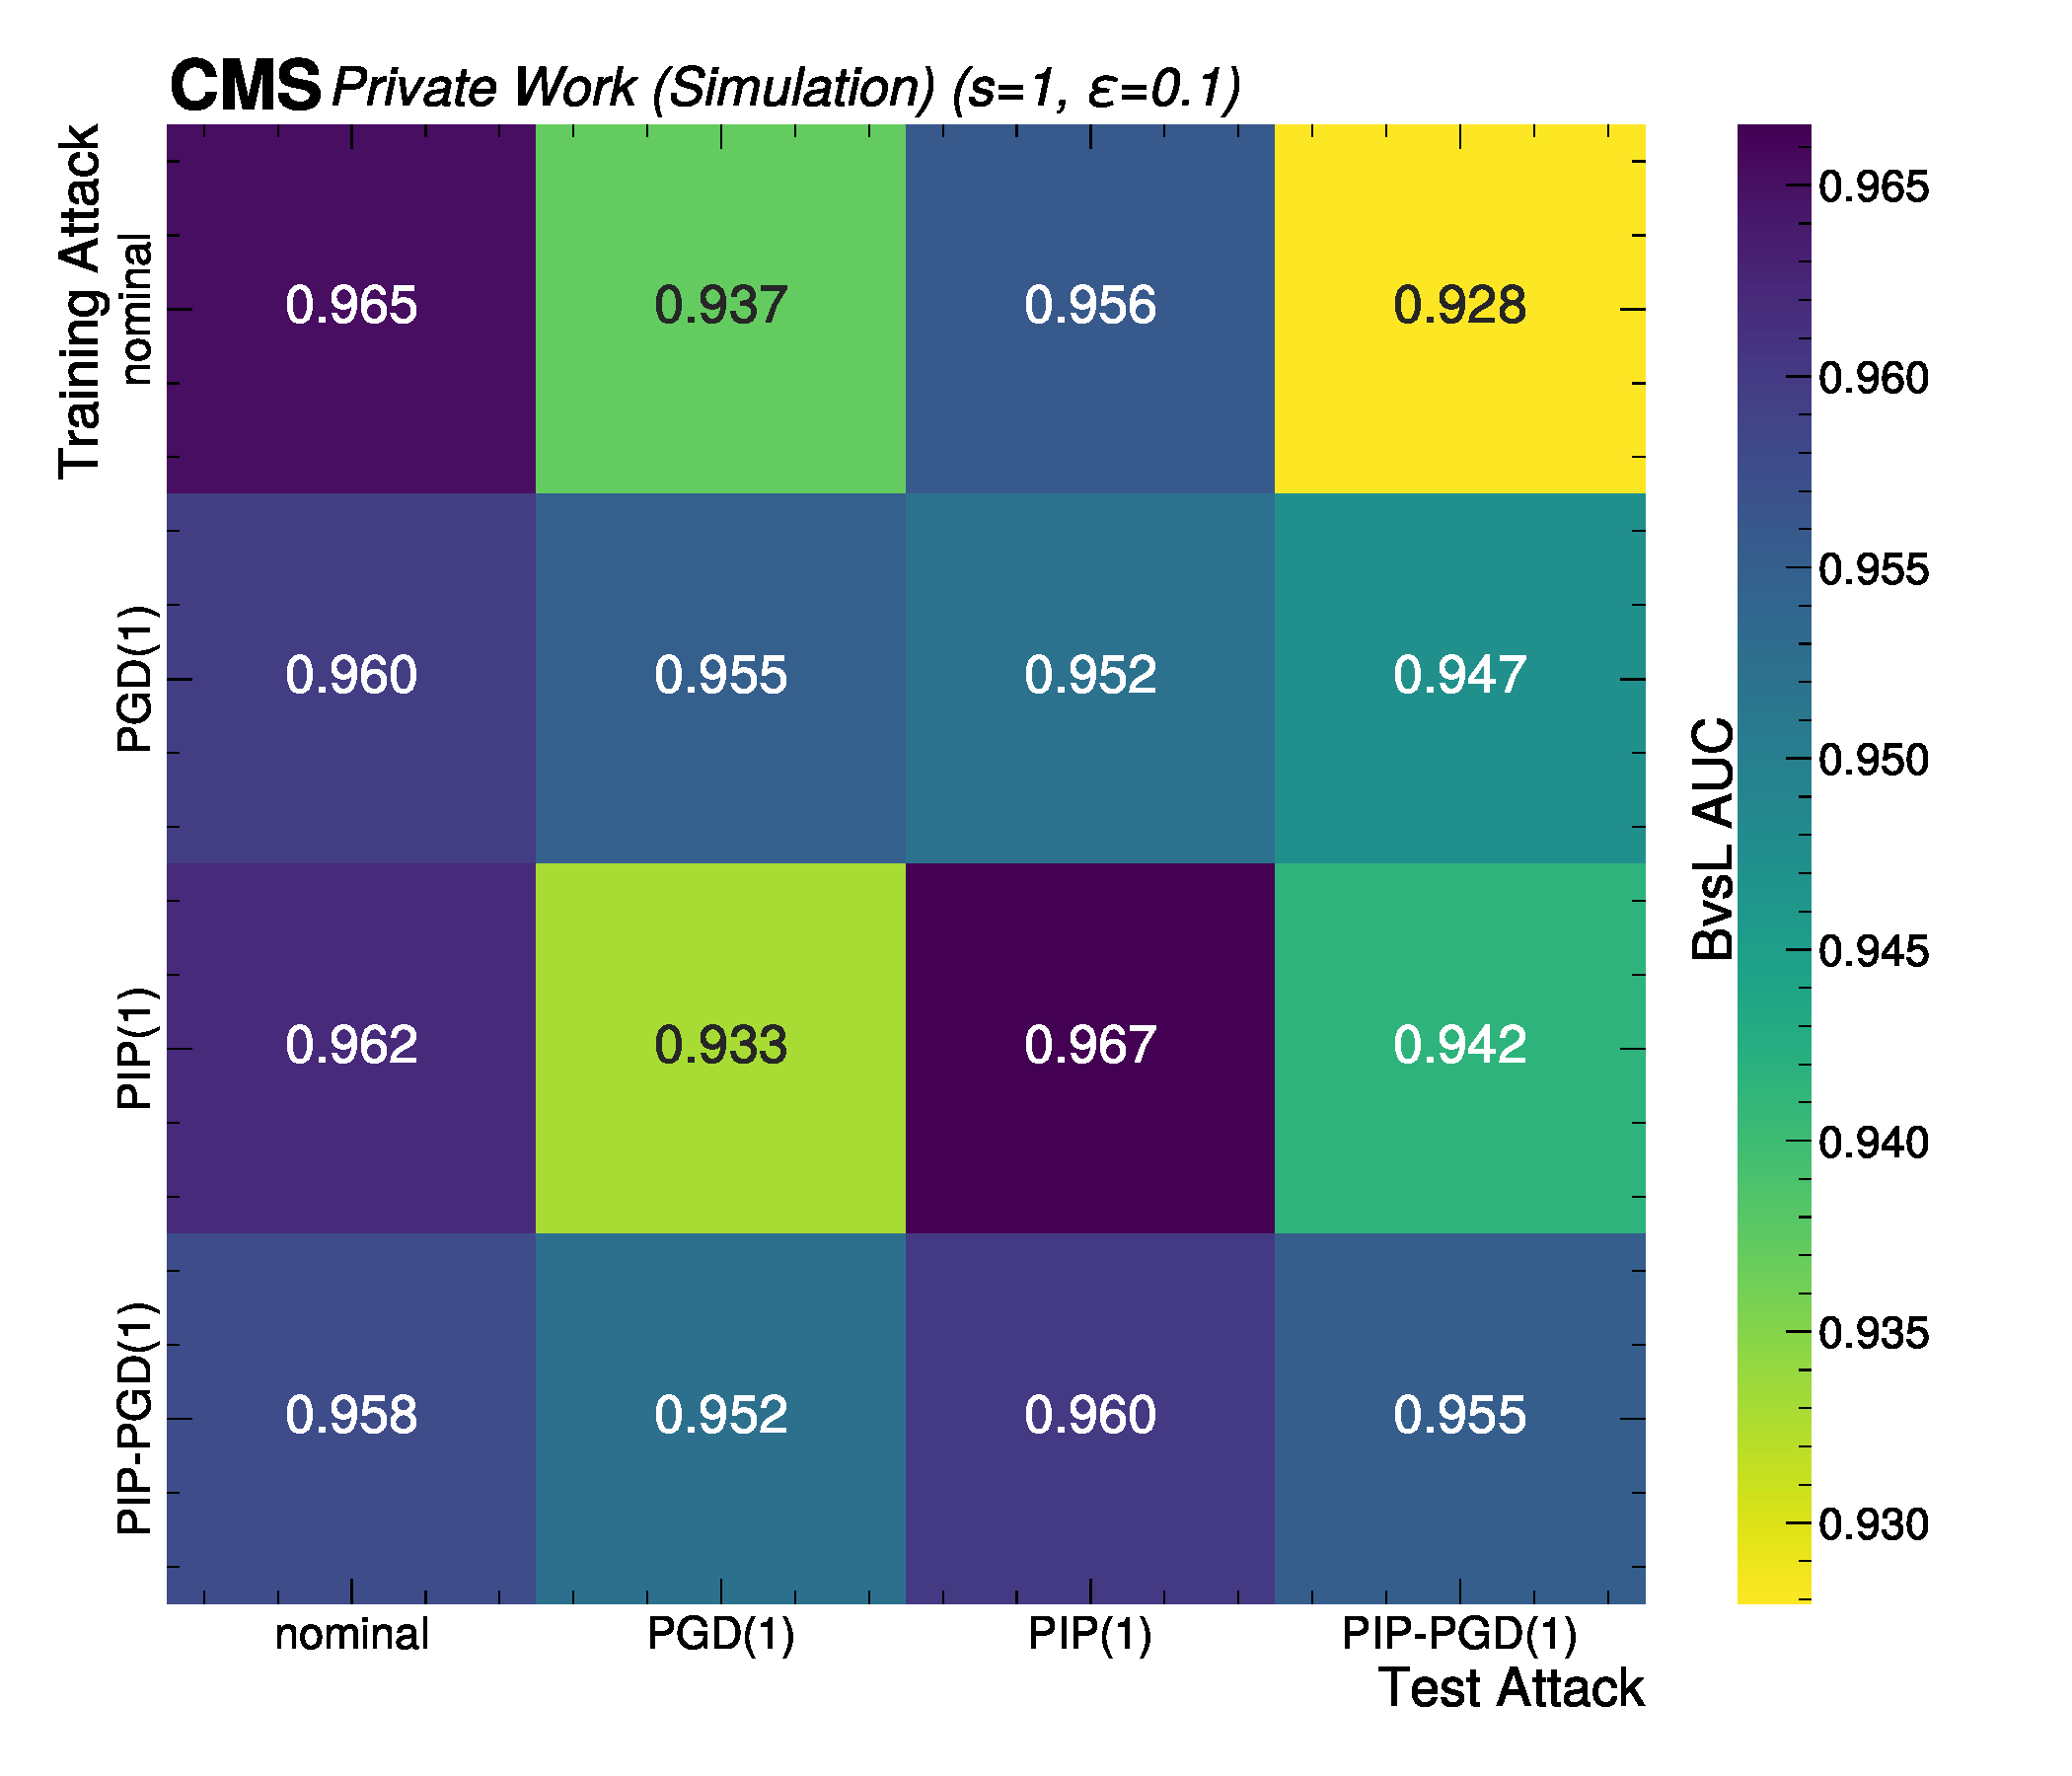
\includegraphics[width=15cm]{media/cross_robustness.pdf}
    \caption{AUC score for BvsL misidentification for all combinations of adversarial training and adversarial testing between nominal, PGD(1), PIP(1), and joint PIP-PGD(1) attacks with a sharpness of $s=1.0$ and $\epsilon=0.1$ while attributing for individual features.}
    \label{fig:cross_robustness}
\end{figure}

Models trained solely on PGD struggle to achieve robustness against integer-based attacks, with an AUC of  $\le0.952$, though they remain stable against PGD perturbations.

Overall, the PIP-PGD training strategy offers the best cross-attack robustness while closely preserving nominal performance, with degradation of approximately 1.3\% for PGD-perturbed data, 0.5\% for PIP-perturbed data, and 1\% for PIP-PGD-perturbed data.

% Chapter 5
\chapter{Conclusion and Outlook}

This thesis has introduced PIP, specifically designed for discrete features in particle physics applications. Applied to the DeepJet flavour tagging algorithm used in CMS, this work demonstrates how to develop a robustness against vulnerabilities in state-of-the-art machine learning models that were previously disregarded.

The key innovation of PIP comes from its probabilistic approach to discrete perturbations without continuous relaxation. Unlike continuous attack methods that generate non-physical fractional values when being applied to integer features, PIP uses gradient information to probabilistically determine whether to increment or decrement discrete features by integer units. This ensures all perturbations remain physically meaningful while effectively probing model robustness. A tunable sharpness parameter controls the attack's aggressiveness, allowing researchers to balance effectiveness with stealth considerations.

The investigation of PIP-PGD attacks reveals synergistic effects exceeding the impact of either method alone. Attacking both, continuous and discrete, features simultaneously exploits complementary vulnerabilities, leading to more severe performance degradation than expected from individual attack impacts.

Adversarial training experiments show that models trained against only one attack type exhibit limited transferability to other attack types, indicating attack-specific overfitting. However, adversarial training with PIP-PGD attacks provides balanced robustness across all tested scenarios while maintaining nominal performance within 1-2\% of baseline levels. This combined training approach offers the most comprehensive protection against both continuous and discrete adversarial perturbations.

Beyond the specific application to DeepJet, this work contributes to the broader field of adversarial machine learning by suggesting a general and computational cheap framework for attacking discrete features on top of continuous values that can be adapted to other scientific domains. The successful combination of continuous and discrete attacks demonstrates the importance of considering multiple perturbation modalities in robustness evaluation, particularly relevant for scientific applications involving mixed data types.

\newpage

While PIP offers a robust method that can be applied in conjunction with existing continuous attack methods, several improvements could enhance its effectiveness. The current implementation does not account for relative feature scaling in the same way that PGD uses feature-specific scaling factors. Incorporating relative scaling based on feature importance or sensitivity has the potential to enhance the efficacy while maintaining physical realism.

The synergy between PGD and PIP could may be attributable to both methods acting on simple gradient information that are generally aligned. However, it remains uncertain whether PIP works equally well with other more sophisticated attack methods. Future research could explore integration with advanced continuous attacks to reveal new synergistic opportunities.

Beyond methodological improvements, PIP could be extended to other scientific machine learning applications where discrete features play important roles. Research areas such as astronomy, materials science, and bioinformatics often involve mixed data types that could benefit from similar robustness analysis approaches. Additionally, incorporating domain-specific knowledge about particle physics has the potential to create more realistic and targeted adversarial perturbations, improving both attack effectiveness and physical interpretability.

\printbibliography

\appendix

% Exclude appendix figures from list of illustrations
\let\oldaddcontentsline\addcontentsline
\renewcommand{\addcontentsline}[3]{%
  \ifnum\pdfstrcmp{#2}{figure}=0
    \ifnum\value{chapter}>0
      % Don't add figures to list of illustrations in appendix
    \else
      \oldaddcontentsline{#1}{#2}{#3}%
    \fi
  \else
    \oldaddcontentsline{#1}{#2}{#3}%
  \fi
}

\chapter{Appendix}

\begin{table}[ht]
\centering
\caption{Evaluation metrics used to quantify model performance and perturbation impact.}
\begin{tabularx}{\textwidth}{@{} l X X @{}}
\toprule
\textbf{Metric} & \textbf{Definition / Calculation} & \textbf{Physical Interpretation} \\
\midrule
\textbf{ROC / AUC} &
The Receiver Operating Characteristic (ROC) curve plots the True Positive Rate (TPR, or sensitivity) against the False Positive Rate (FPR) across varying classification thresholds. The Area Under the Curve (AUC) is the integral of the ROC curve, ranging from 0.5 (random classifier) to 1.0 (perfect classifier). &
The ROC curve illustrates the trade-off between correctly identifying heavy-flavour jets (TPR) and mistakenly tagging background jets (FPR). A higher AUC indicates better model performance in distinguishing signal from background, critical for robust jet tagging. \\
\addlinespace
\textbf{\(\Delta\)AUC (AUC Drop)} &
Difference in the model’s Area Under the ROC Curve (AUC) between nominal (unperturbed) and adversarial datasets. Often reported as a percentage of the nominal AUC. &
Measures the loss of discriminative power for jet tagging. A larger drop means the adversarial attack significantly degrades the classifier’s ability to distinguish heavy-flavour jets from background (attack success). \\
\addlinespace
\textbf{Jensen–Shannon Distance (JSD)} &
The square root of the Jensen–Shannon divergence between the distribution of a given feature for nominal vs. attacked samples (see Equation~(\ref{eq:jsd})). Computed on each feature’s 1D histogram, excluding default/padding values. &
Quantifies the \emph{statistical difference} between original and perturbed feature distributions. Low JSD (near 0) indicates minimal change (stealthy), while high JSD reveals visible distribution shifts. \\
\hline
\end{tabularx}
\label{tab:evaluation_metrics}
\end{table}



\begin{figure}[h]
\centering
    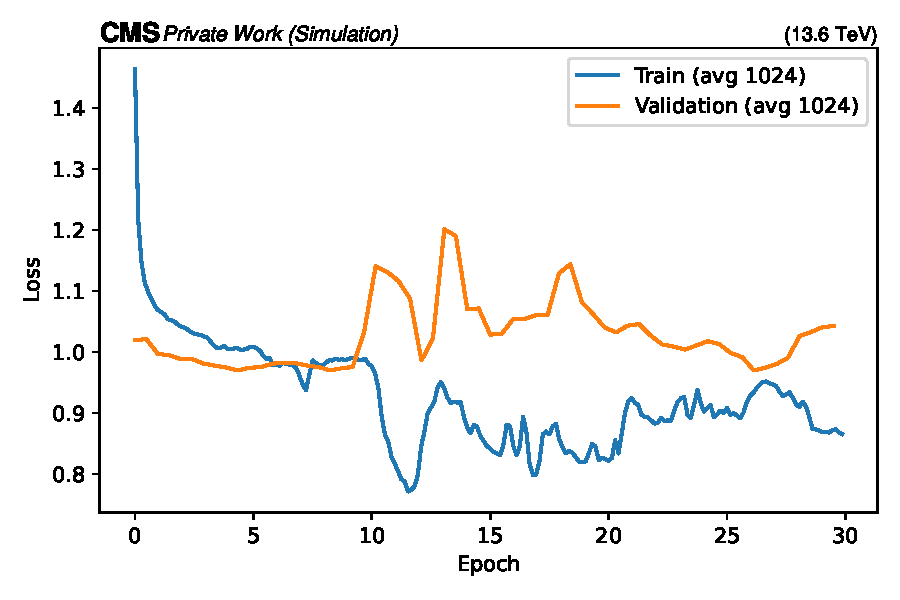
\includegraphics[width=13cm]{media/output/intpgd_loss_validation.pdf}
    \caption{Training and validation loss for FGSM applied to the entire input spectrum training.}
    \label{fig:intpgd_train}
\end{figure}

\section{Input Features}

% Table for global input features
\begin{table}[ht]
\centering
\caption{Descriptions of the global input features with applied masks $\mathcal{M_{\text{float}}}$, $\mathcal{M_{\text{int}}}$, $\mathcal{M_{\text{int}}^*\subset M_{\text{int}}}$.}
\begin{tabularx}{\textwidth}{|c|c|X|c|}
\hline
\textbf{variable name} & \textbf{type} & \textbf{description} & \textbf{mask} \\
\hline
\texttt{jet\_pt} & float & transverse momentum of the jet in GeV & \cellcolor{green!50}$\mathcal{M_{\text{float}}}$ \\
\hline
\texttt{jet\_eta} & float & pseudorapidity of the jet & \cellcolor{green!50}$\mathcal{M_{\text{float}}}$ \\
\hline
\texttt{n\_Cpfcand} & int & number of charged PF candidates in the jet & \cellcolor{orange!50}$\mathcal{M_{\text{int}}}$ \\
\hline
\texttt{n\_Npfcand} & int & number of neutral PF candidates in the jet & \cellcolor{orange!50}$\mathcal{M_{\text{int}}}$ \\
\hline
\texttt{nsv} & int & number of secondary vertices in the jet & \cellcolor{orange!50}$\mathcal{M_{\text{int}}}$ \\
\hline
\texttt{npv} & int & number of primary vertices in the event & \cellcolor{orange!50}$\mathcal{M_{\text{int}}}$ \\
\hline
\texttt{TagVarCSV\_trackSumJetEtRatio} & float & transverse energy ratio of tracks and jet & \cellcolor{green!50}$\mathcal{M_{\text{float}}}$ \\
\hline
\texttt{TagVarCSV\_trackSumJetDeltaR} & float & spatial distance between the sum of tracks and jet axis & \cellcolor{green!50}$\mathcal{M_{\text{float}}}$ \\
\hline
\texttt{TagVarCSV\_vertexCategory} & int & secondary vertex category index & \cellcolor{orange!50}$\mathcal{M_{\text{int}}}$ \\
\hline
\texttt{TagVarCSV\_trackSip2dValAboveCharm} & float & 2D signed impact parameter of first track lifting mass above charm in cm & \cellcolor{green!50}$\mathcal{M_{\text{float}}}$ \\
\hline
\texttt{TagVarCSV\_trackSip2dSigAboveCharm} & float & 2D signed impact parameter significance of first track lifting mass above charm & \cellcolor{green!50}$\mathcal{M_{\text{float}}}$ \\
\hline
\texttt{TagVarCSV\_trackSip3dValAboveCharm} & float & 3D signed impact parameter of first track lifting mass above charm in cm & \cellcolor{green!50}$\mathcal{M_{\text{float}}}$ \\
\hline
\texttt{TagVarCSV\_trackSip3dSigAboveCharm} & float & 3D signed impact parameter significance of first track lifting mass above charm & \cellcolor{green!50}$\mathcal{M_{\text{float}}}$ \\
\hline
\texttt{TagVarCSV\_jetNSelectedTracks} & int & number of tracks associated to jet & \cellcolor{orange!50}$\mathcal{M_{\text{int}}}$ \\
\hline
\texttt{TagVarCSV\_jetNTracksEtaRel} & int & number of tracks associated to jet for which \( \eta_{\text{rel}} \) is computed & \cellcolor{orange!50}$\mathcal{M_{\text{int}}}$ \\
\hline
\end{tabularx}
\label{tab:global_input_features}
\end{table}


% Table for CPF input features
\begin{table}[ht]
\centering
\caption{Descriptions of the CPF input features with applied masks $\mathcal{M_{\text{float}}}$, $\mathcal{M_{\text{int}}}$, $\mathcal{M_{\text{int}}^*\subset M_{\text{int}}}$.}
\begin{tabularx}{\textwidth}{|c|c|X|c|}
\hline
\textbf{variable name} & \textbf{type} & \textbf{description} & \textbf{mask} \\
\hline
\texttt{Cpfcan\_BtagPf\_trackEtaRel} & float & pseudorapidity of charged track relative to jet axis & \cellcolor{green!50}$\mathcal{M_{\text{float}}}$ \\
\hline
\texttt{Cpfcan\_BtagPf\_trackPtRel} & float & momentum of charged track transverse to jet axis in GeV & \cellcolor{green!50}$\mathcal{M_{\text{float}}}$ \\
\hline
\texttt{Cpfcan\_BtagPf\_trackPPar} & float & momentum of charged track along jet axis in GeV & \cellcolor{green!50}$\mathcal{M_{\text{float}}}$ \\
\hline
\texttt{Cpfcan\_BtagPf\_trackDeltaR} & float & spatial distance between track and jet axis & \cellcolor{green!50}$\mathcal{M_{\text{float}}}$ \\
\hline
\texttt{Cpfcan\_BtagPf\_trackPParRatio} & float & momentum fraction of charged track along jet axis & \cellcolor{green!50}$\mathcal{M_{\text{float}}}$ \\
\hline
\texttt{Cpfcan\_BtagPf\_trackSip2dVal} & float & 2D signed impact parameter of charged track in cm & \cellcolor{green!50}$\mathcal{M_{\text{float}}}$ \\
\hline
\texttt{Cpfcan\_BtagPf\_trackSip2dSig} & float & 2D signed impact parameter significance of charged track & \cellcolor{green!50}$\mathcal{M_{\text{float}}}$ \\
\hline
\texttt{Cpfcan\_BtagPf\_trackSip3dVal} & float & 3D signed impact parameter of charged track in cm & \cellcolor{green!50}$\mathcal{M_{\text{float}}}$ \\
\hline
\texttt{Cpfcan\_BtagPf\_trackSip3dSig} & float & 3D signed impact parameter significance of charged track & \cellcolor{green!50}$\mathcal{M_{\text{float}}}$ \\
\hline
\texttt{Cpfcan\_BtagPf\_trackJetDistVal} & float & minimum distance between track and jet axis & \cellcolor{green!50}$\mathcal{M_{\text{float}}}$ \\
\hline
\texttt{Cpfcan\_ptrel} & float & transverse momentum fraction of the track & \cellcolor{green!50}$\mathcal{M_{\text{float}}}$ \\
\hline
\texttt{Cpfcan\_drminsv} & float & spatial distance between the track and the closest secondary vertex & \cellcolor{green!50}$\mathcal{M_{\text{float}}}$ \\
\hline
\texttt{Cpfcan\_VTX\_ass} & int & integer flag: usage of track in primary vertex fit & \cellcolor{orange!50}$\mathcal{M_{\text{int}}}^*$ \\
\hline
\texttt{Cpfcan\_puppiw} & int & PUPPI weight of the charged PF candidate & \cellcolor{red!50}$\mathcal{M_{\text{int}}}$ \\
\hline
\texttt{Cpfcan\_chi2} & int & \( \chi^2 \) of charged track fit & \cellcolor{red!50}$\mathcal{M_{\text{int}}}$ \\
\hline
\texttt{Cpfcan\_quality} & int & integer flag: quality of fitted track & \cellcolor{orange!50}$\mathcal{M_{\text{int}}}^*$ \\
\hline
\end{tabularx}
\label{tab:cpf_input_features}
\end{table}


% Table for NPF input features
\begin{table}[ht]
\centering
\caption{Descriptions of the NPF input features with applied masks $\mathcal{M_{\text{float}}}$, $\mathcal{M_{\text{int}}}$, $\mathcal{M_{\text{int}}^*\subset M_{\text{int}}}$.}
\begin{tabularx}{\textwidth}{|c|c|X|c|}
\hline
\textbf{variable name} & \textbf{type} & \textbf{description} & \textbf{mask} \\
\hline
\texttt{Npfcan\_ptrel} & float & transverse momentum fraction of the track & \cellcolor{green!50}$\mathcal{M_{\text{float}}}$ \\
\hline
\texttt{Npfcan\_deltaR} & float & spatial distance between track and jet axis & \cellcolor{green!50}$\mathcal{M_{\text{float}}}$ \\
\hline
\texttt{Npfcan\_isGamma} & int & integer flag: particle identity (1 = photon, 0 = no photon) & \cellcolor{orange!50}$\mathcal{M_{\text{int}}}^*$ \\
\hline
\texttt{Npfcan\_HadFrac} & int & fraction of the energy deposited in the hadronic calorimeter & \cellcolor{orange!50}$\mathcal{M_{\text{int}}}^*$ \\
\hline
\texttt{Npfcan\_drminsv} & float & spatial distance between the track and the closest secondary vertex & \cellcolor{green!50}$\mathcal{M_{\text{float}}}$ \\
\hline
\texttt{Npfcan\_puppiw} & int & PUPPI weight of the neutral PF candidate & \cellcolor{red!50}$\mathcal{M_{\text{int}}}$ \\
\hline
\end{tabularx}
\label{tab:npf_input_features}
\end{table}


% Table for SV input features
\begin{table}[ht]
\centering
\caption{Descriptions of the SV input features with applied masks $\mathcal{M_{\text{float}}}$, $\mathcal{M_{\text{int}}}$, $\mathcal{M_{\text{int}}^*\subset M_{\text{int}}}$.}
\begin{tabularx}{\textwidth}{|c|c|X|c|}
\hline
\textbf{variable name} & \textbf{data type} & \textbf{description} & \textbf{mask} \\
\hline
\texttt{sv\_pt} & float & transverse momentum of the SV in GeV & \cellcolor{green!50}$\mathcal{M_{\text{float}}}$ \\
\hline
\texttt{sv\_deltaR} & float & spatial distance between SV and jet axis & \cellcolor{green!50}$\mathcal{M_{\text{float}}}$ \\
\hline
\texttt{sv\_mass} & float & mass of the SV in GeV & \cellcolor{green!50}$\mathcal{M_{\text{float}}}$ \\
\hline
\texttt{sv\_ntracks} & int & number of tracks associated to the SV & \cellcolor{red!50}$\mathcal{M_{\text{int}}}$ \\
\hline
\texttt{sv\_chi2} & int & \( \chi^2 \) of the SV fit & \cellcolor{red!50}$\mathcal{M_{\text{int}}}$ \\
\hline
\texttt{sv\_normchi2} & int & \( \chi^2 \) divided by the degrees of freedom & \cellcolor{red!50}$\mathcal{M_{\text{int}}}$ \\
\hline
\texttt{sv\_dxy} & float & 2D flight distance of SV in cm & \cellcolor{green!50}$\mathcal{M_{\text{float}}}$ \\
\hline
\texttt{sv\_dxysig} & float & 2D flight distance significance of SV & \cellcolor{green!50}$\mathcal{M_{\text{float}}}$ \\
\hline
\texttt{sv\_d3d} & float & 3D flight distance of SV in cm & \cellcolor{green!50}$\mathcal{M_{\text{float}}}$ \\
\hline
\texttt{sv\_d3dsig} & float & 3D flight distance significance of SV & \cellcolor{green!50}$\mathcal{M_{\text{float}}}$ \\
\hline
\texttt{sv\_costhetasvpv} & float & cosine of the angle between SV flight direction and SV momentum & \cellcolor{green!50}$\mathcal{M_{\text{float}}}$ \\
\hline
\texttt{sv\_enratio} & float & energy fraction of the SV & \cellcolor{green!50}$\mathcal{M_{\text{float}}}$ \\
\hline
\end{tabularx}
\label{tab:sv_input_features}
\end{table}


\section{PIP Input Similarities}
\label{appendix:intprob}

\subsection*{Global Features}

\begin{figure}[h]
  \centering
  \begin{subfigure}[t]{0.32\textwidth}
    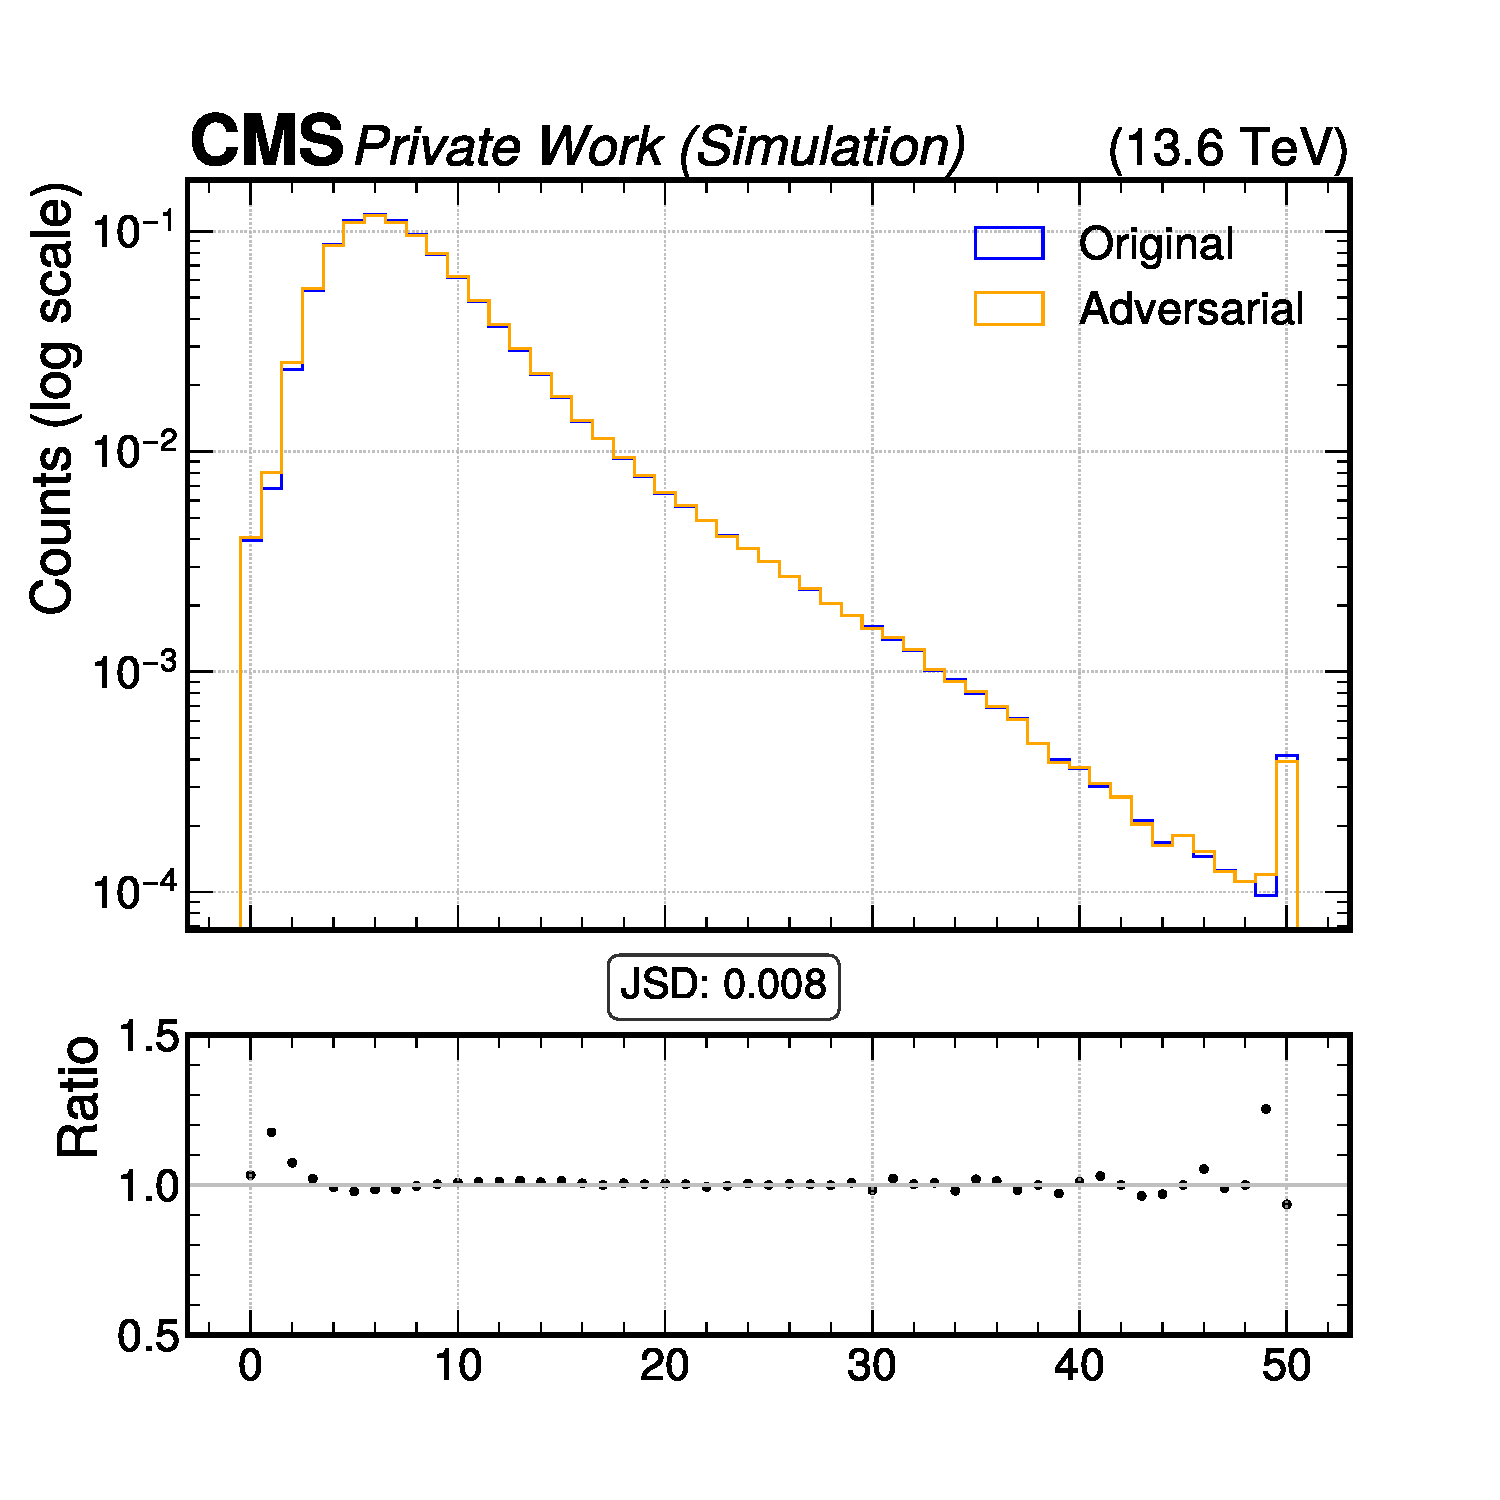
\includegraphics[width=\linewidth]{media/output/features/compare/intprob_1/cmp_global_features_n_Cpfcand.pdf}
    \caption{Input similarity for PIP(1).}
  \end{subfigure}\hfill
  \begin{subfigure}[t]{0.32\textwidth}
    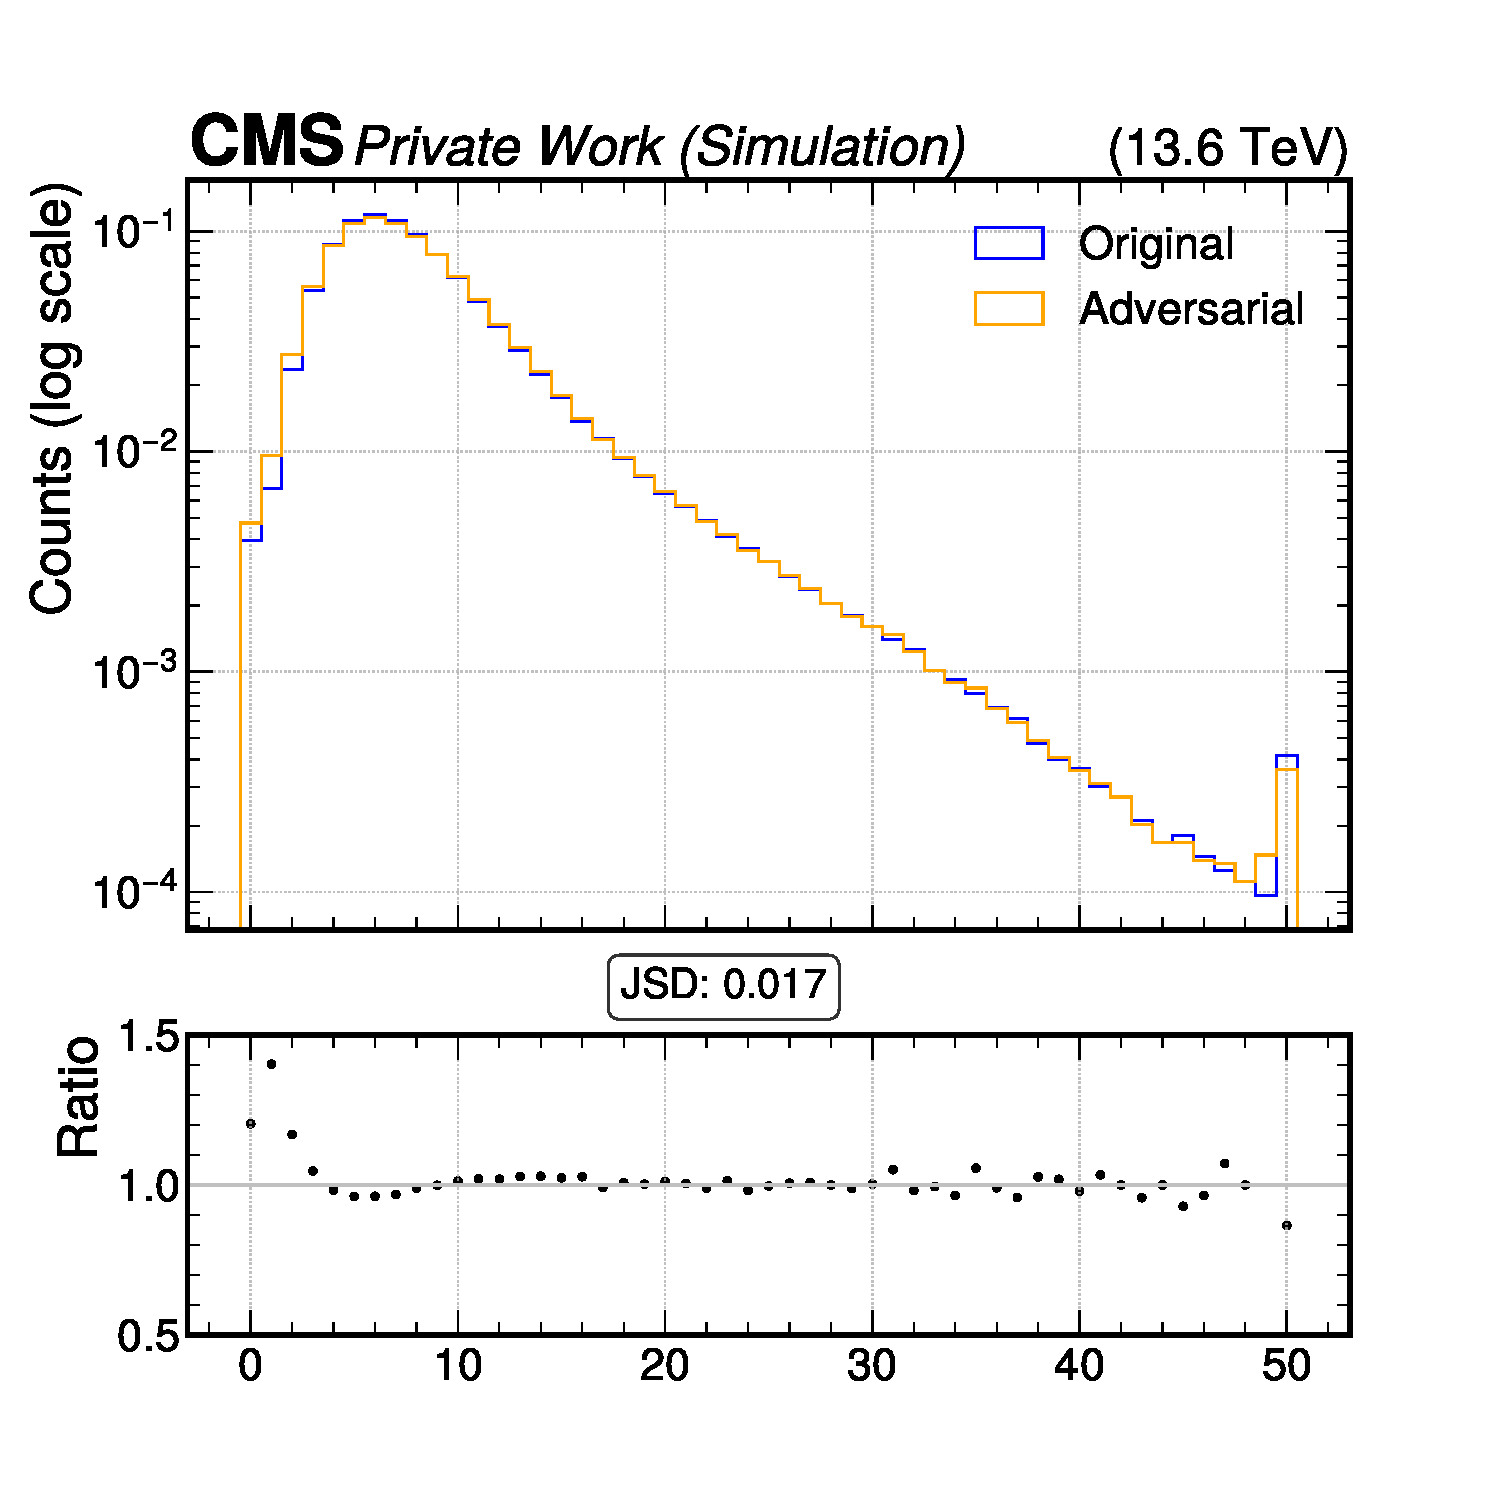
\includegraphics[width=\linewidth]{media/output/features/compare/intprob_2/cmp_global_features_n_Cpfcand.pdf}
    \caption{Input similarity for PIP(2).}
  \end{subfigure}\hfill
  \begin{subfigure}[t]{0.32\textwidth}
    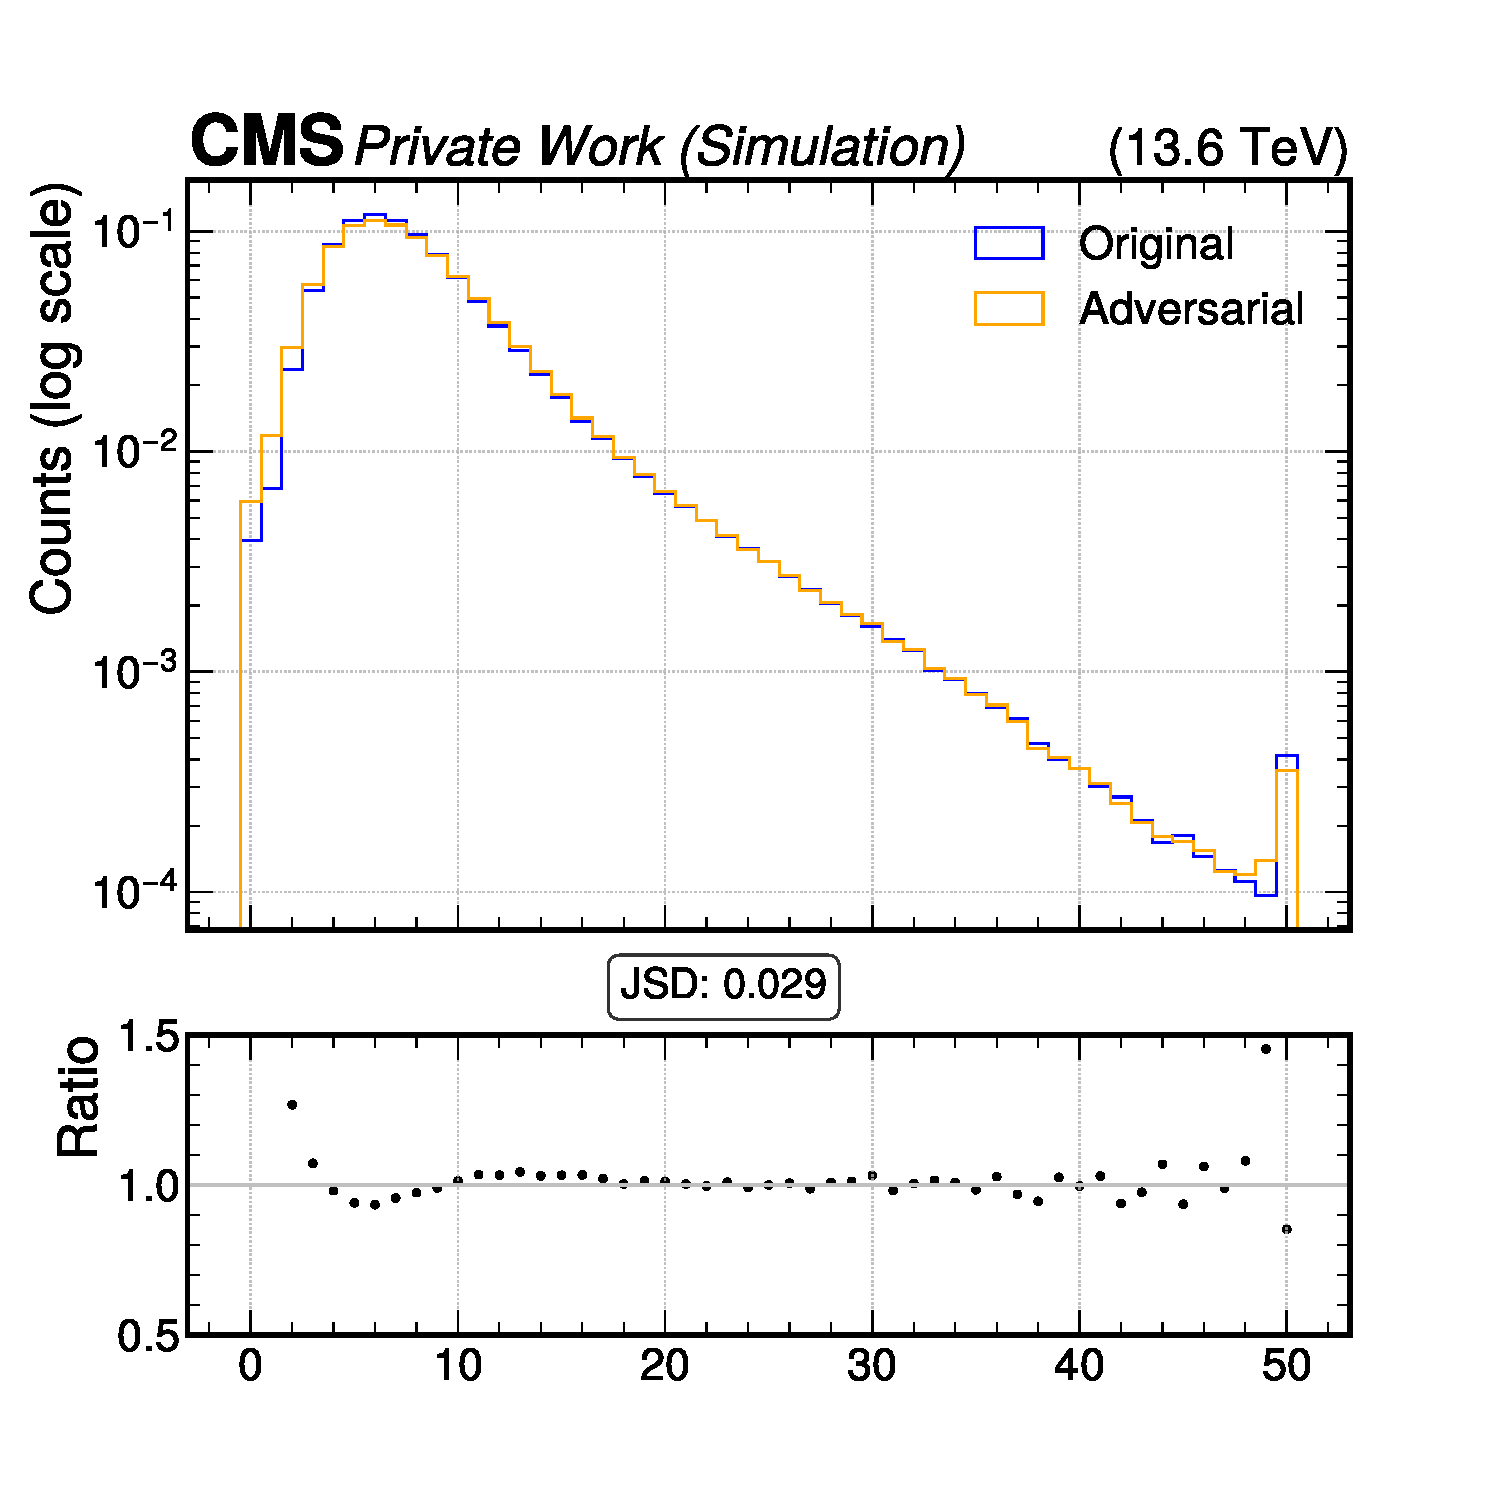
\includegraphics[width=\linewidth]{media/output/features/compare/intprob_3/cmp_global_features_n_Cpfcand.pdf}
    \caption{Input similarity for PIP(3).}
  \end{subfigure}

  \caption{Histogram for \texttt{n\_Cpfcand} for multiple iterations of PIP tested against nominal inputs.}
  \label{fig:intprob_input_n_Cpfcand}
\end{figure}
\begin{figure}[h]
  \centering
  \begin{subfigure}[t]{0.32\textwidth}
    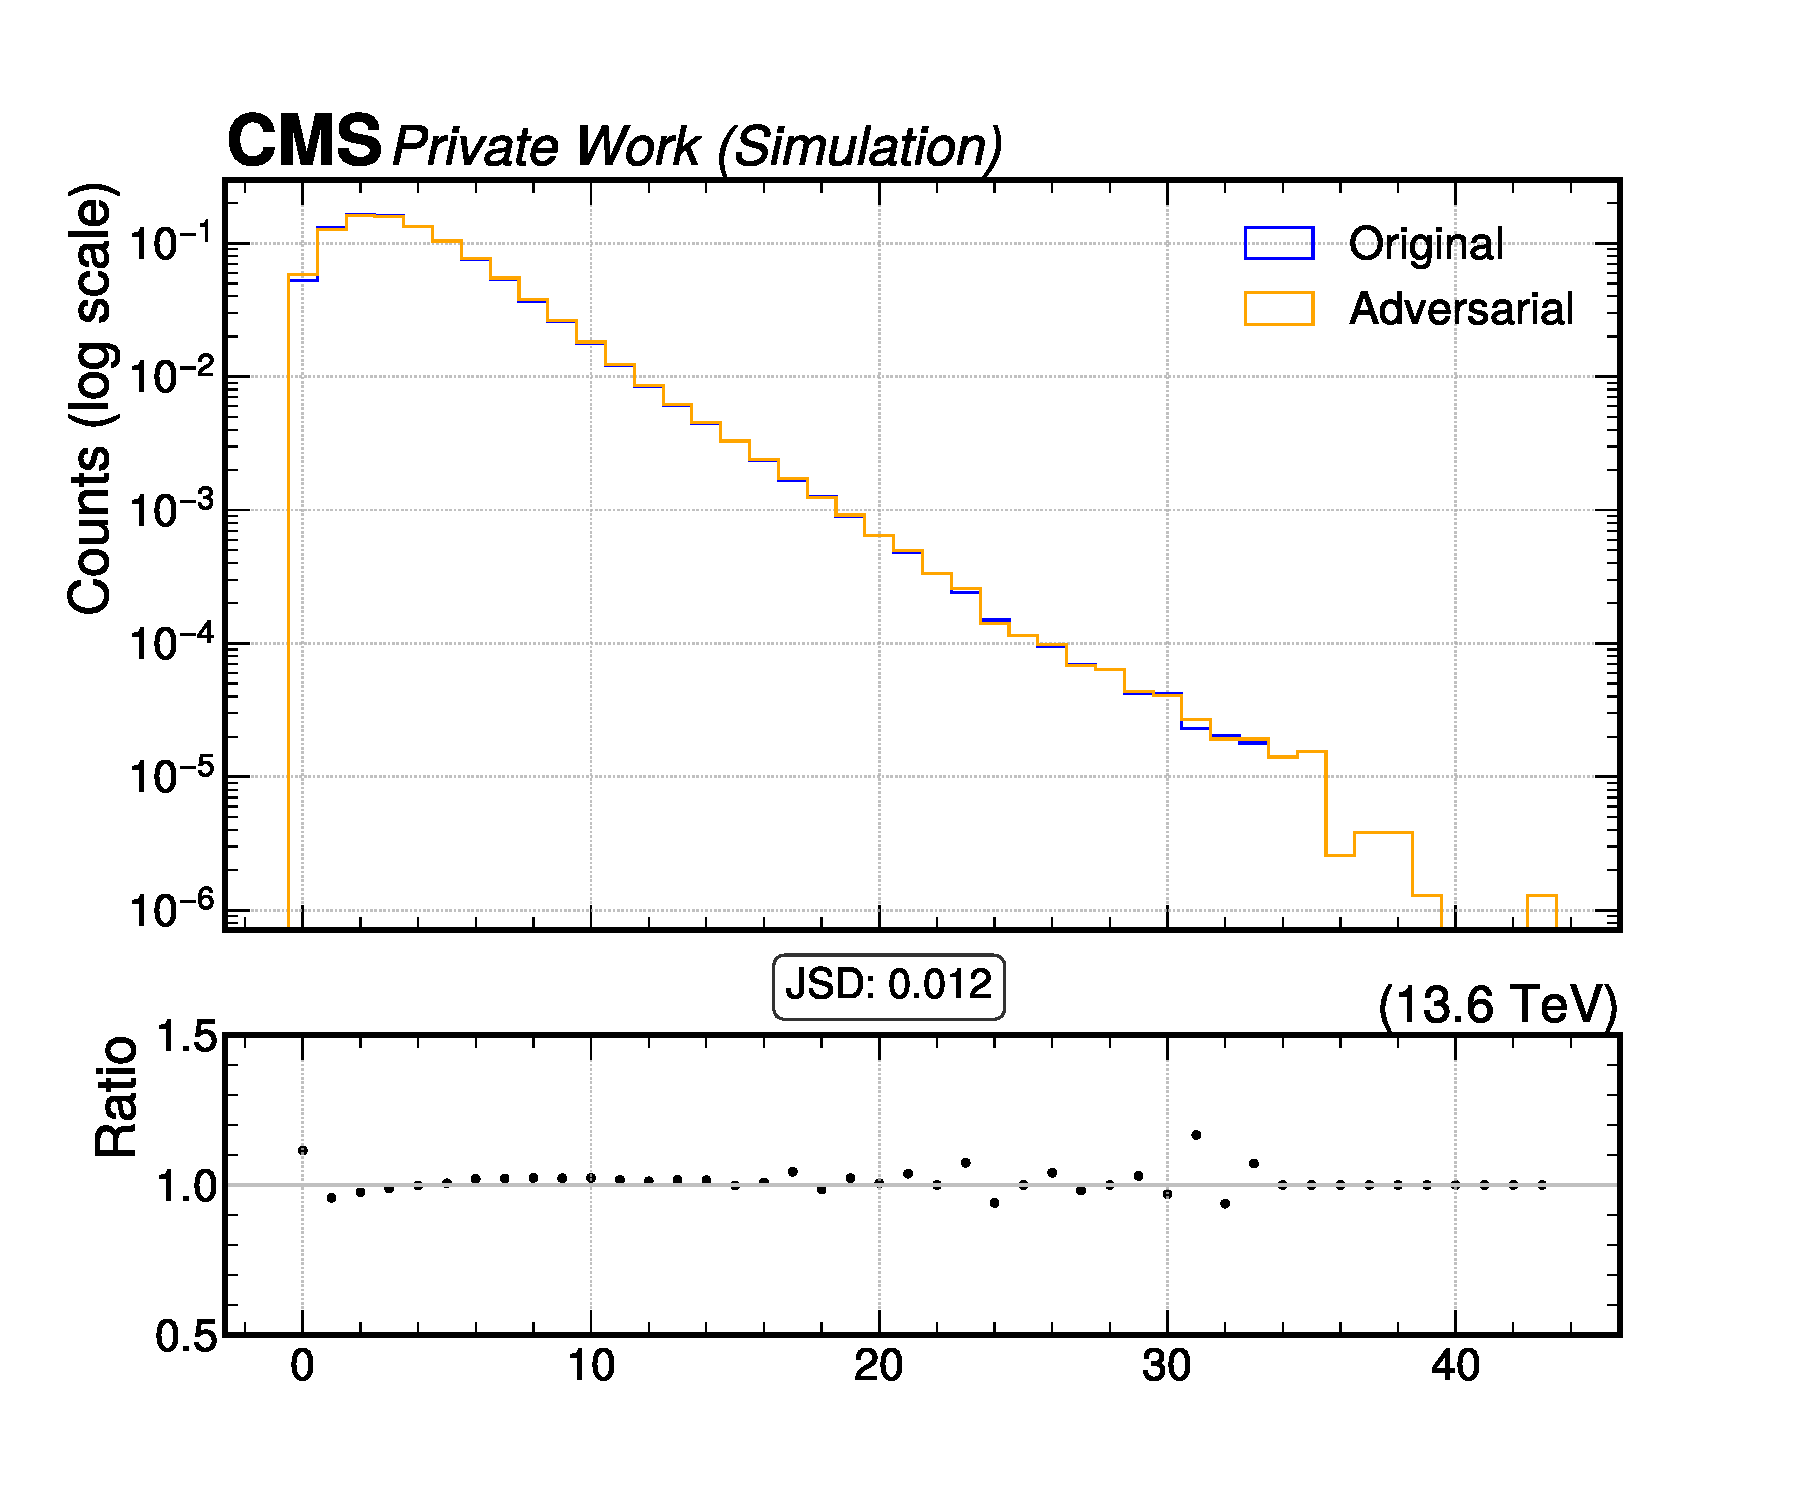
\includegraphics[width=\linewidth]{media/output/features/compare/intprob_1/cmp_global_features_n_Npfcand.pdf}
    \caption{Input similarity for PIP(1).}
  \end{subfigure}\hfill
  \begin{subfigure}[t]{0.32\textwidth}
    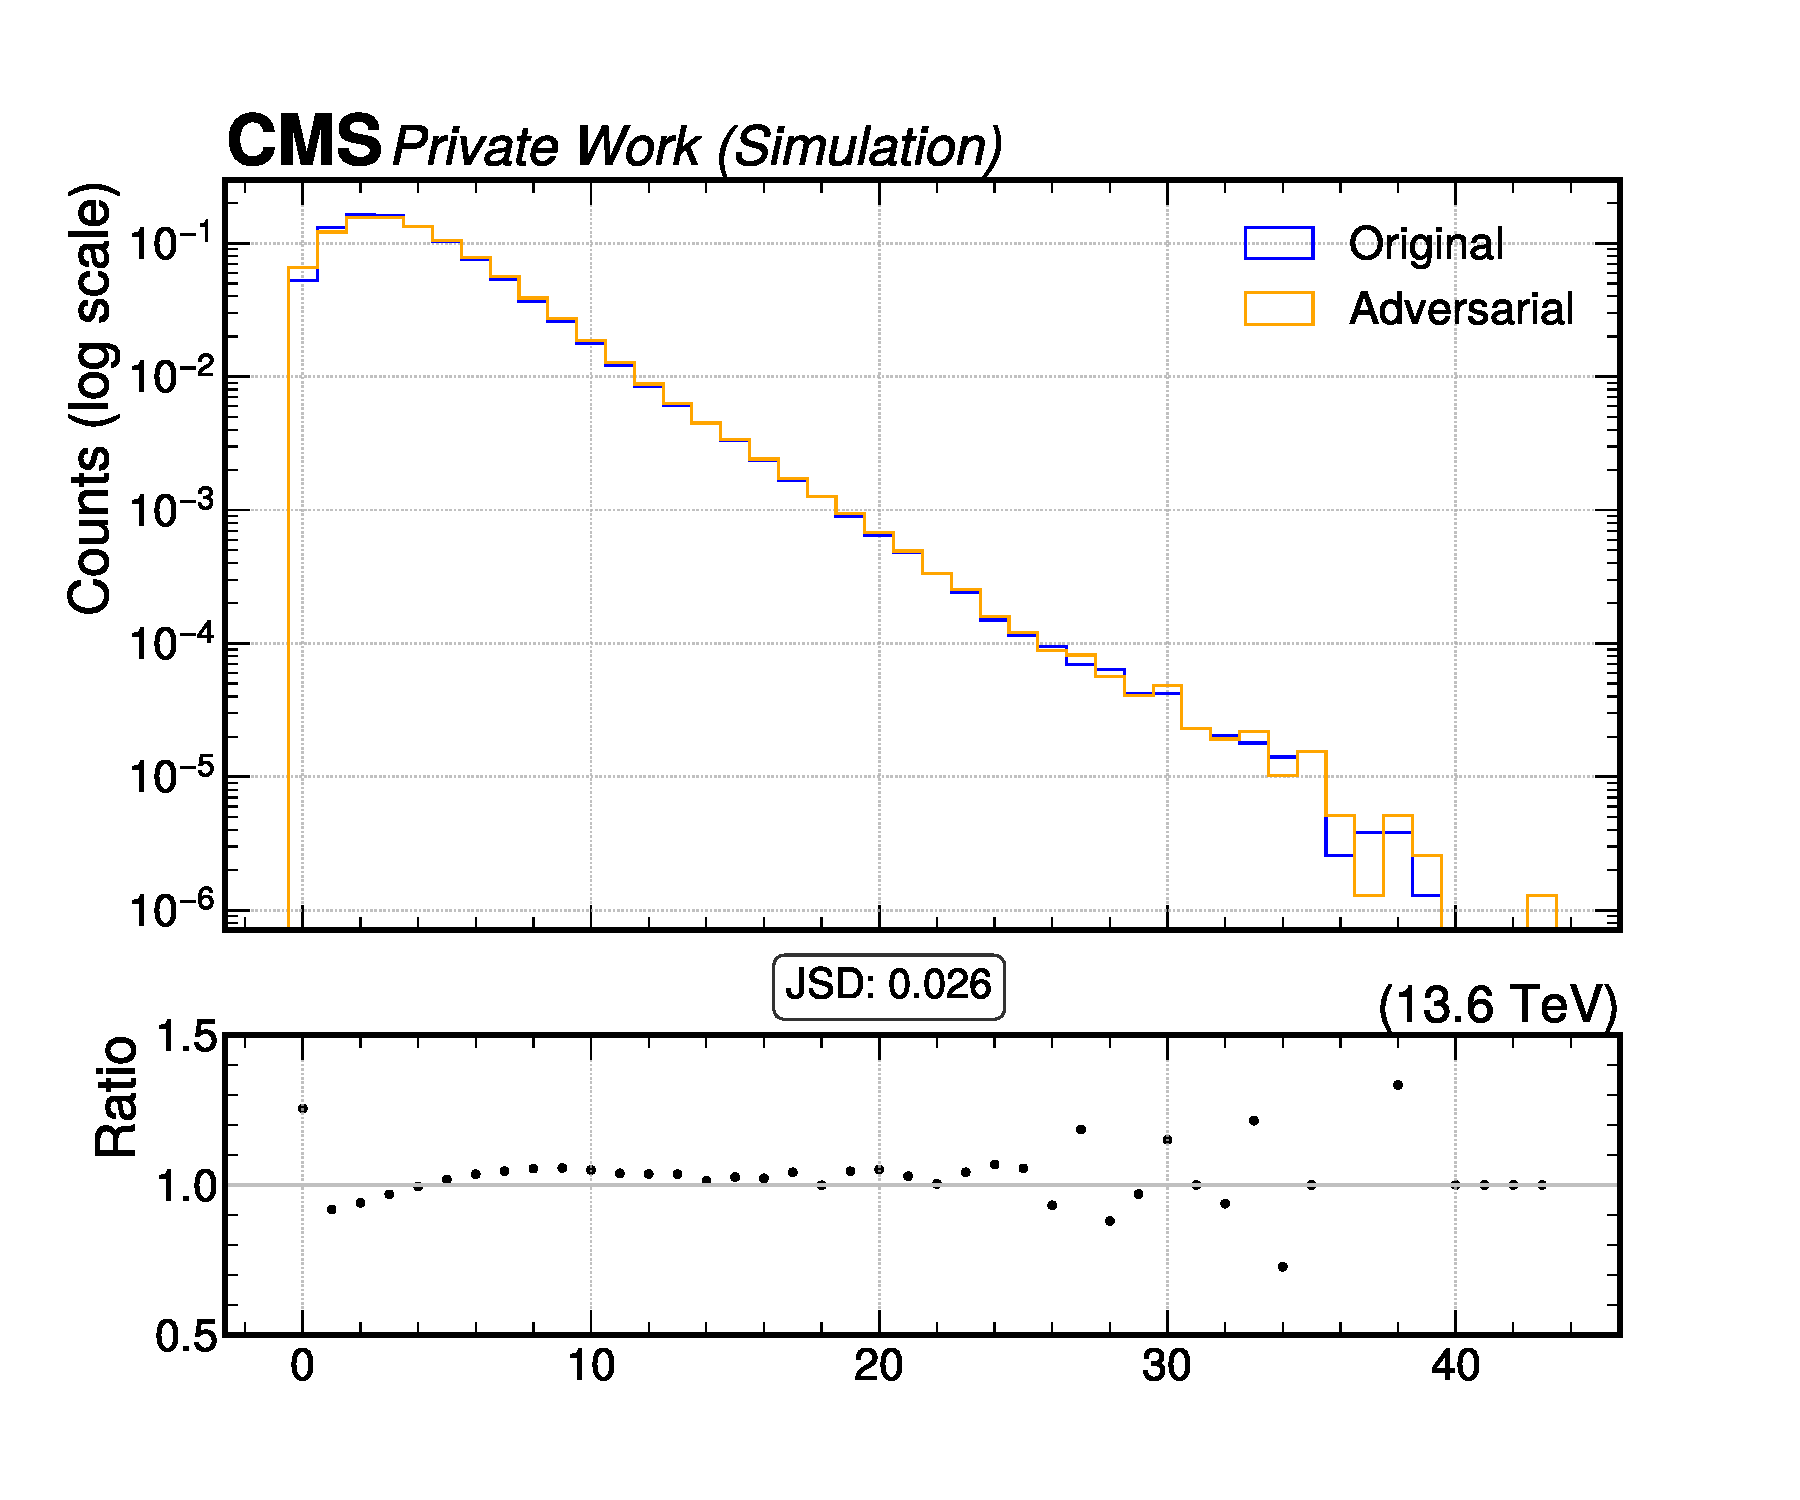
\includegraphics[width=\linewidth]{media/output/features/compare/intprob_2/cmp_global_features_n_Npfcand.pdf}
    \caption{Input similarity for PIP(2).}
  \end{subfigure}\hfill
  \begin{subfigure}[t]{0.32\textwidth}
    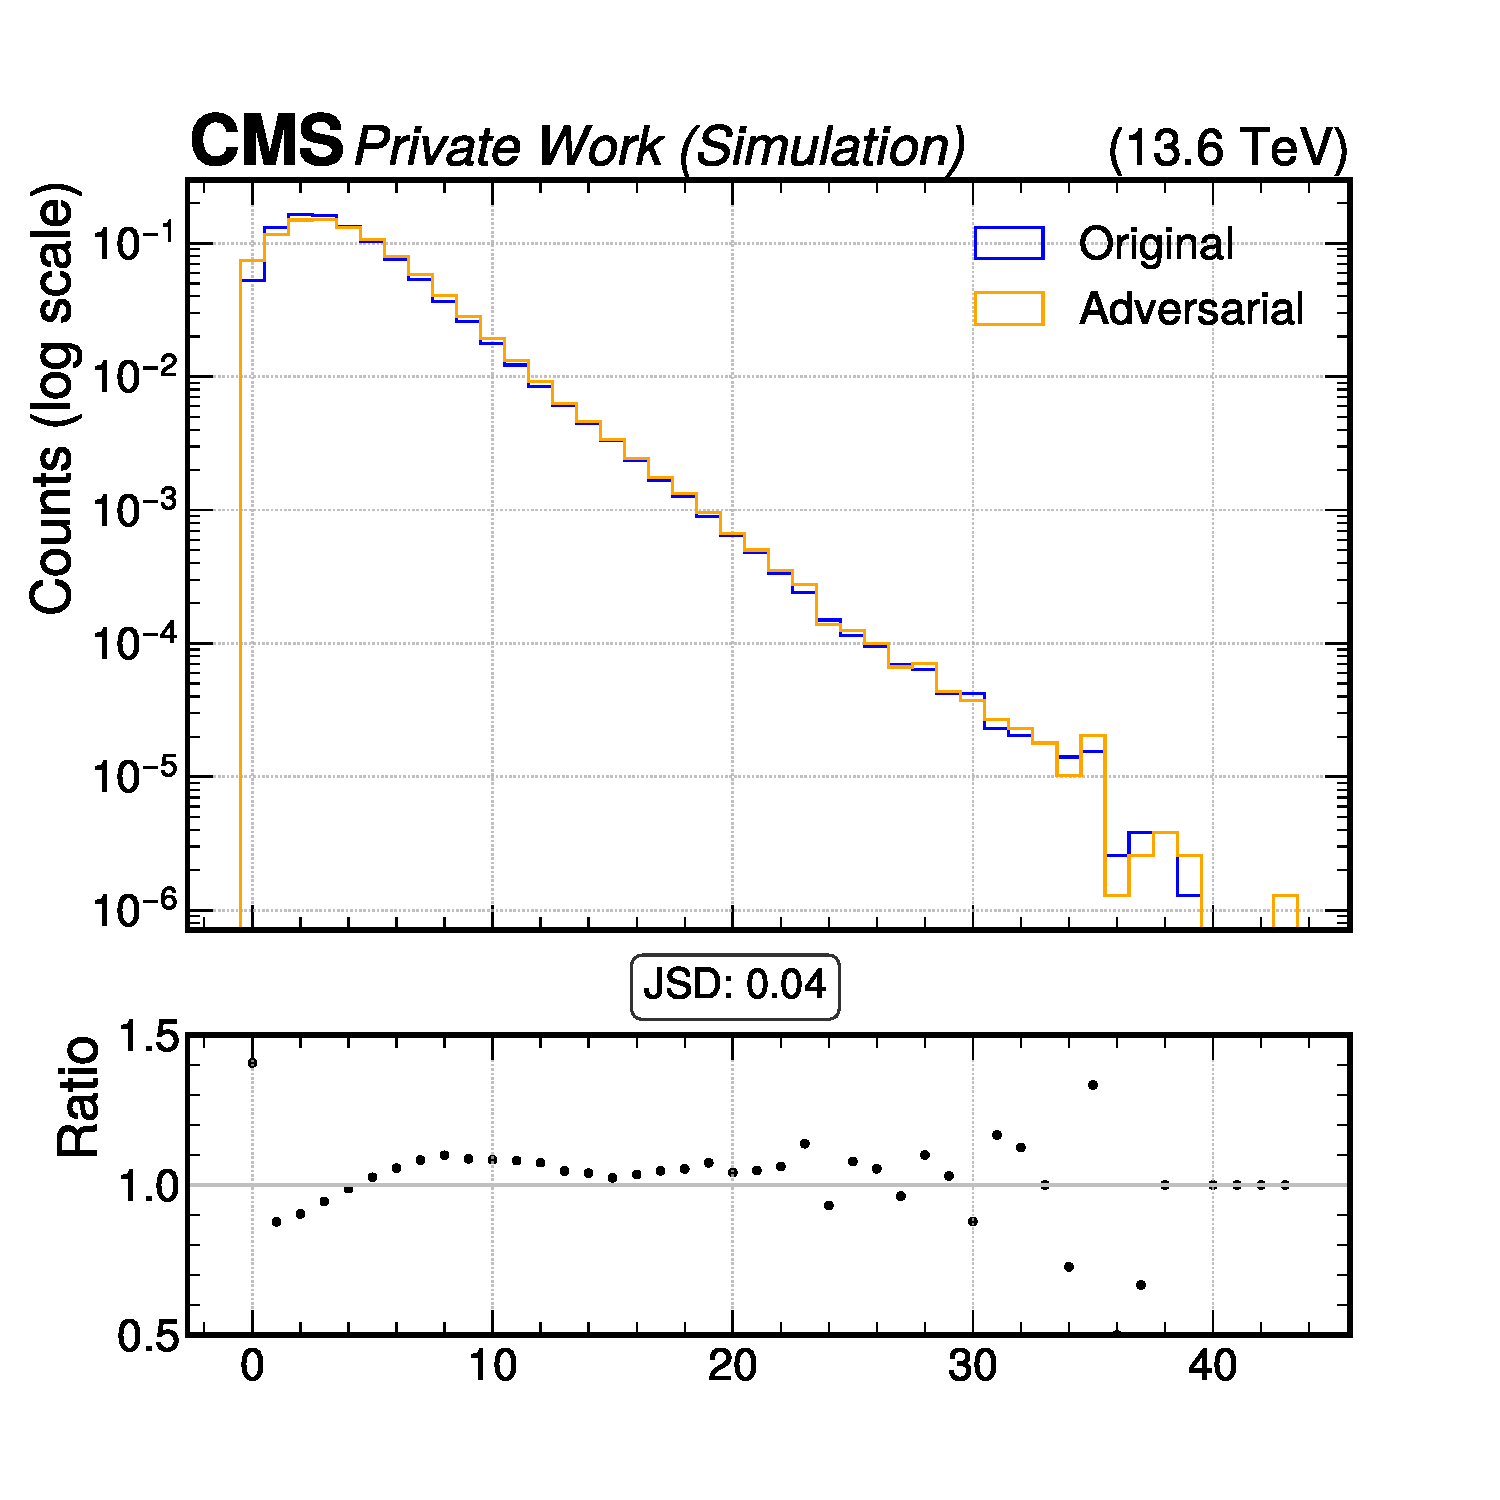
\includegraphics[width=\linewidth]{media/output/features/compare/intprob_3/cmp_global_features_n_Npfcand.pdf}
    \caption{Input similarity for PIP(3).}
  \end{subfigure}

  \caption{Histogram for \texttt{n\_Npfcand} for multiple iterations of PIP tested against nominal inputs.}
  \label{fig:intprob_input_n_Npfcand}
\end{figure}
\begin{figure}[h]
  \centering
  \begin{subfigure}[t]{0.32\textwidth}
    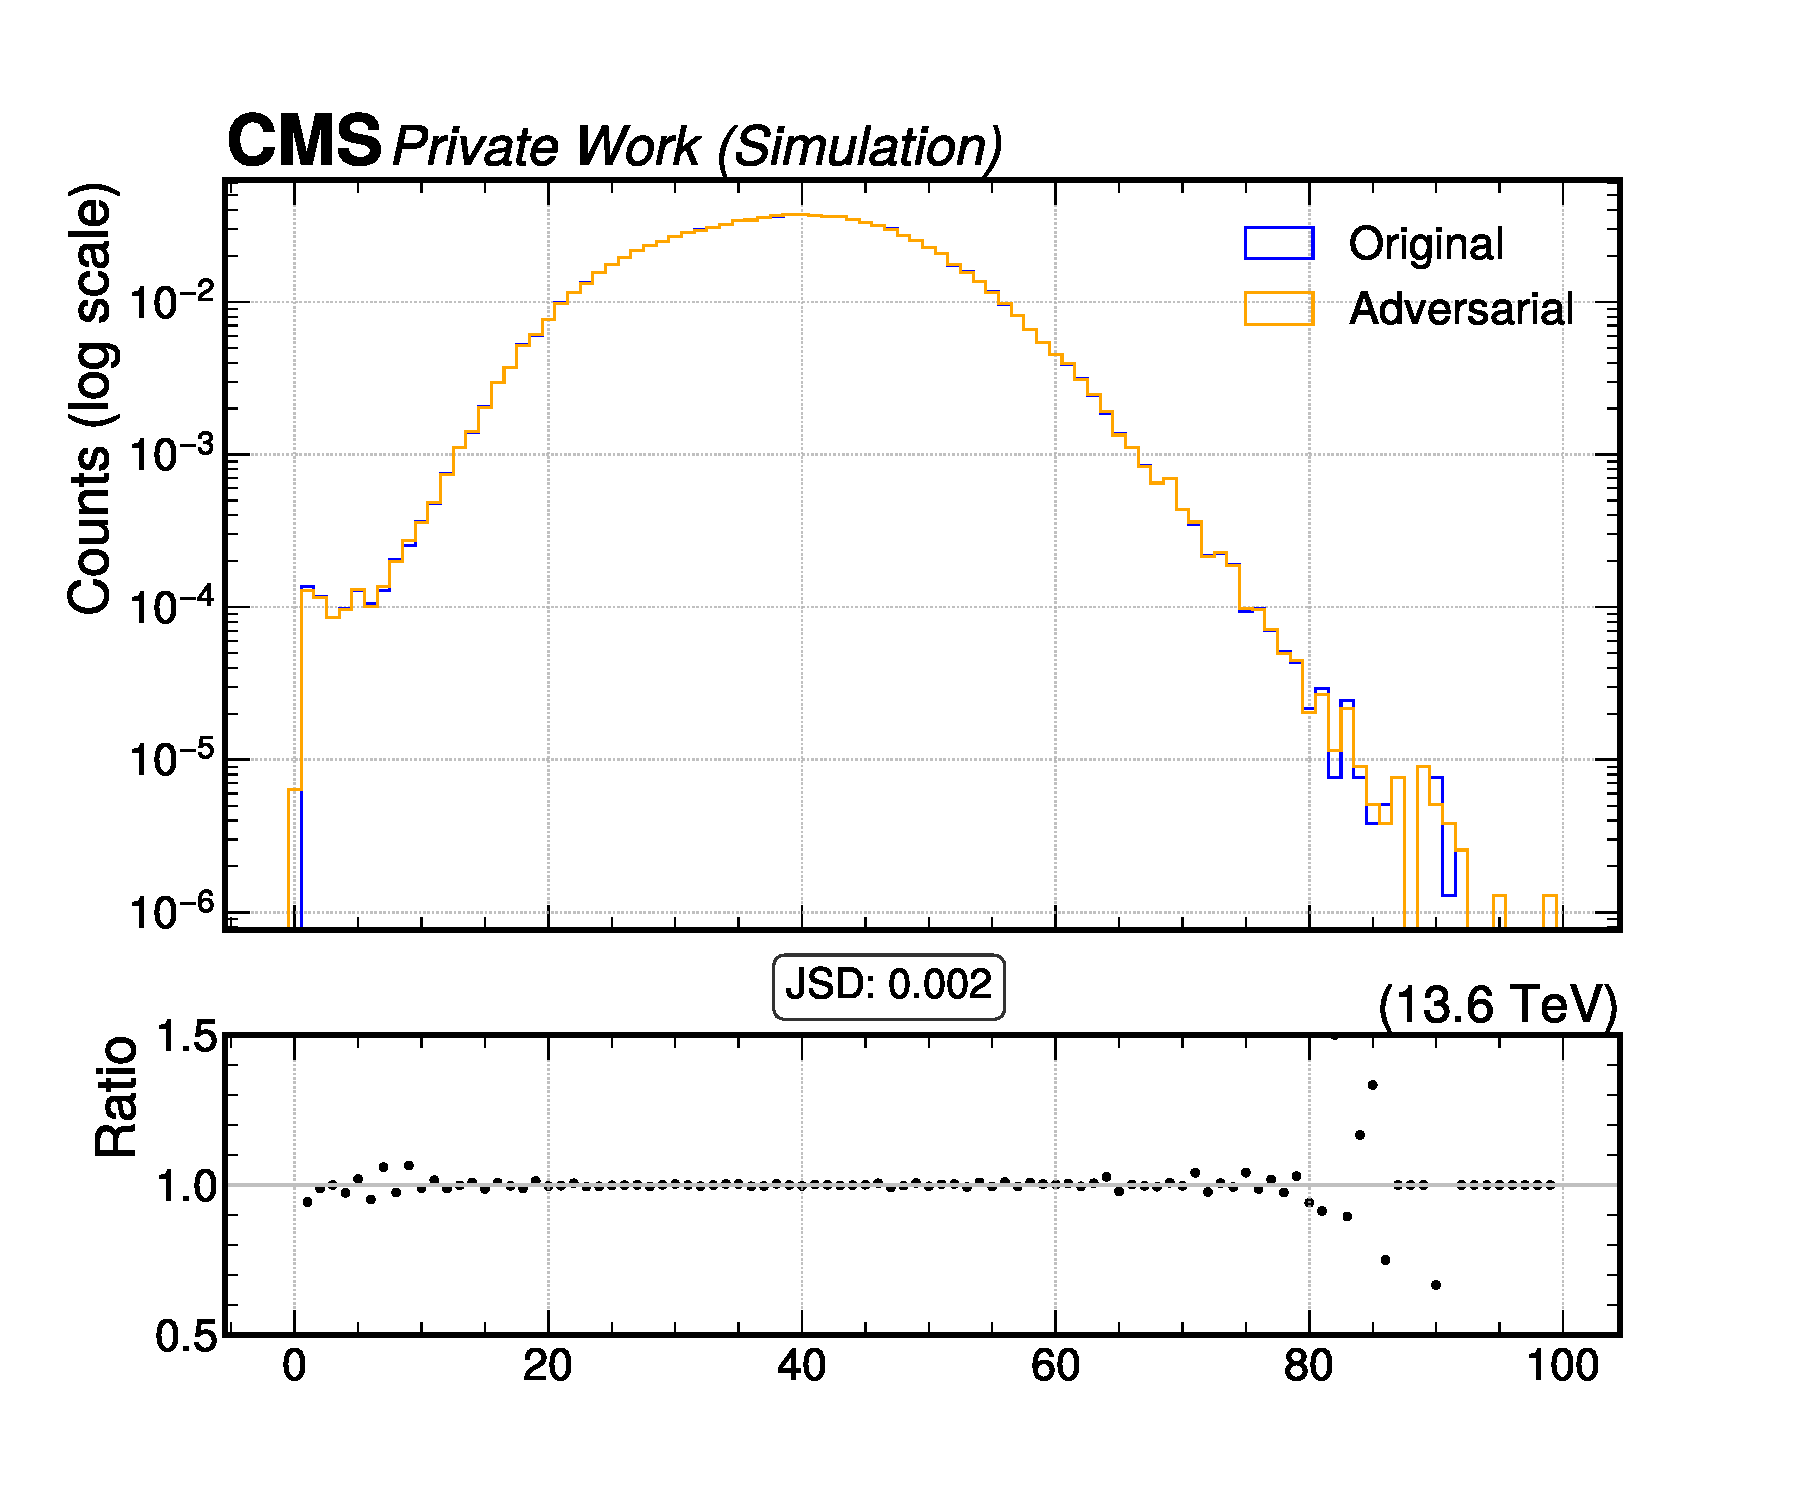
\includegraphics[width=\linewidth]{media/output/features/compare/intprob_1/cmp_global_features_npv.pdf}
    \caption{Input similarity for PIP(1).}
  \end{subfigure}\hfill
  \begin{subfigure}[t]{0.32\textwidth}
    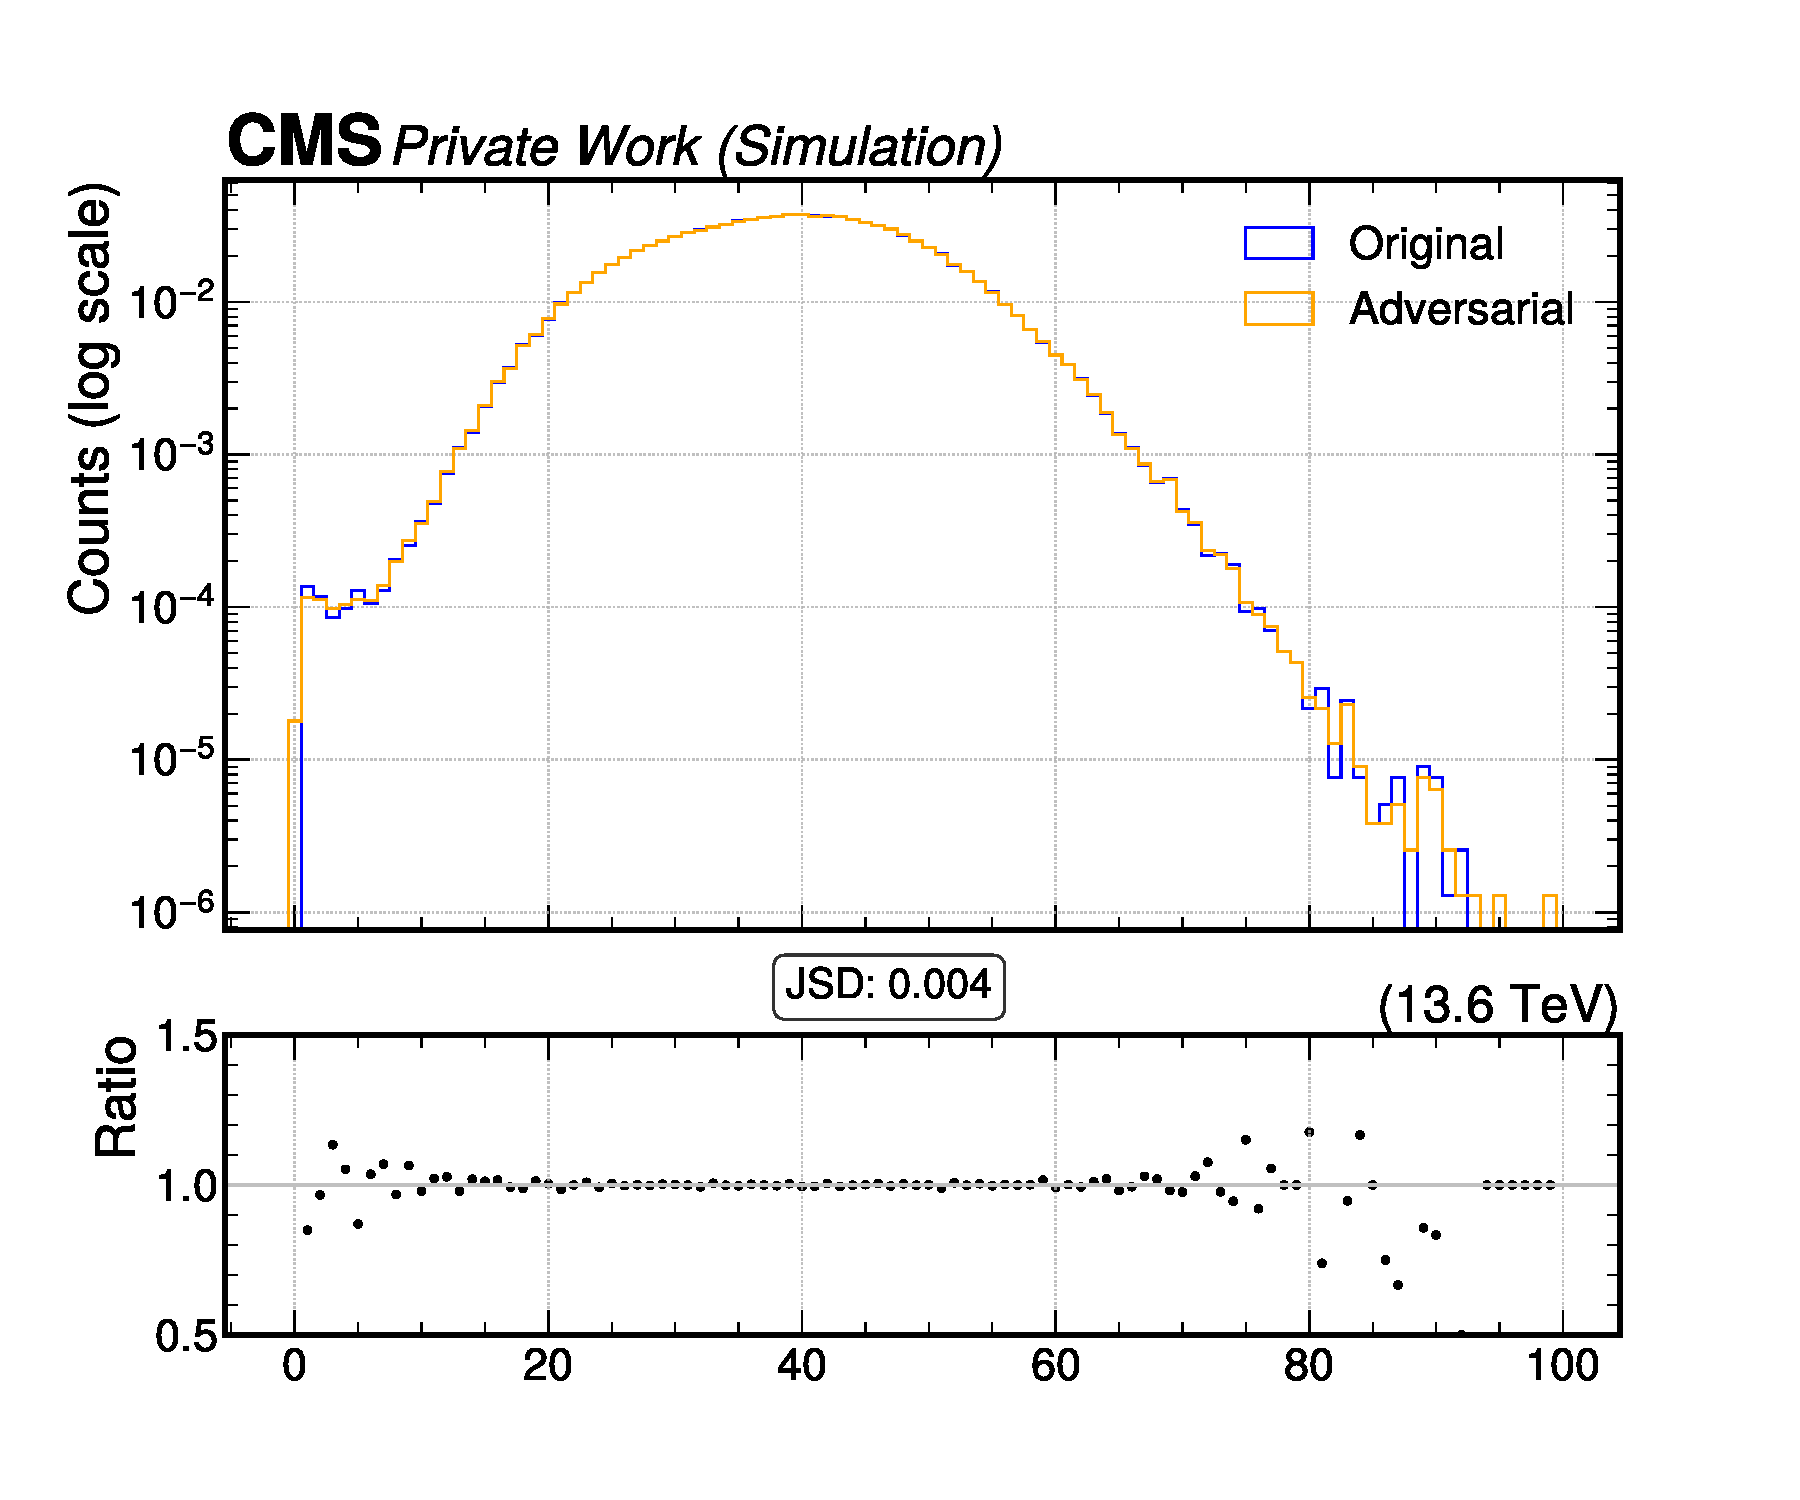
\includegraphics[width=\linewidth]{media/output/features/compare/intprob_2/cmp_global_features_npv.pdf}
    \caption{Input similarity for PIP(2).}
  \end{subfigure}\hfill
  \begin{subfigure}[t]{0.32\textwidth}
    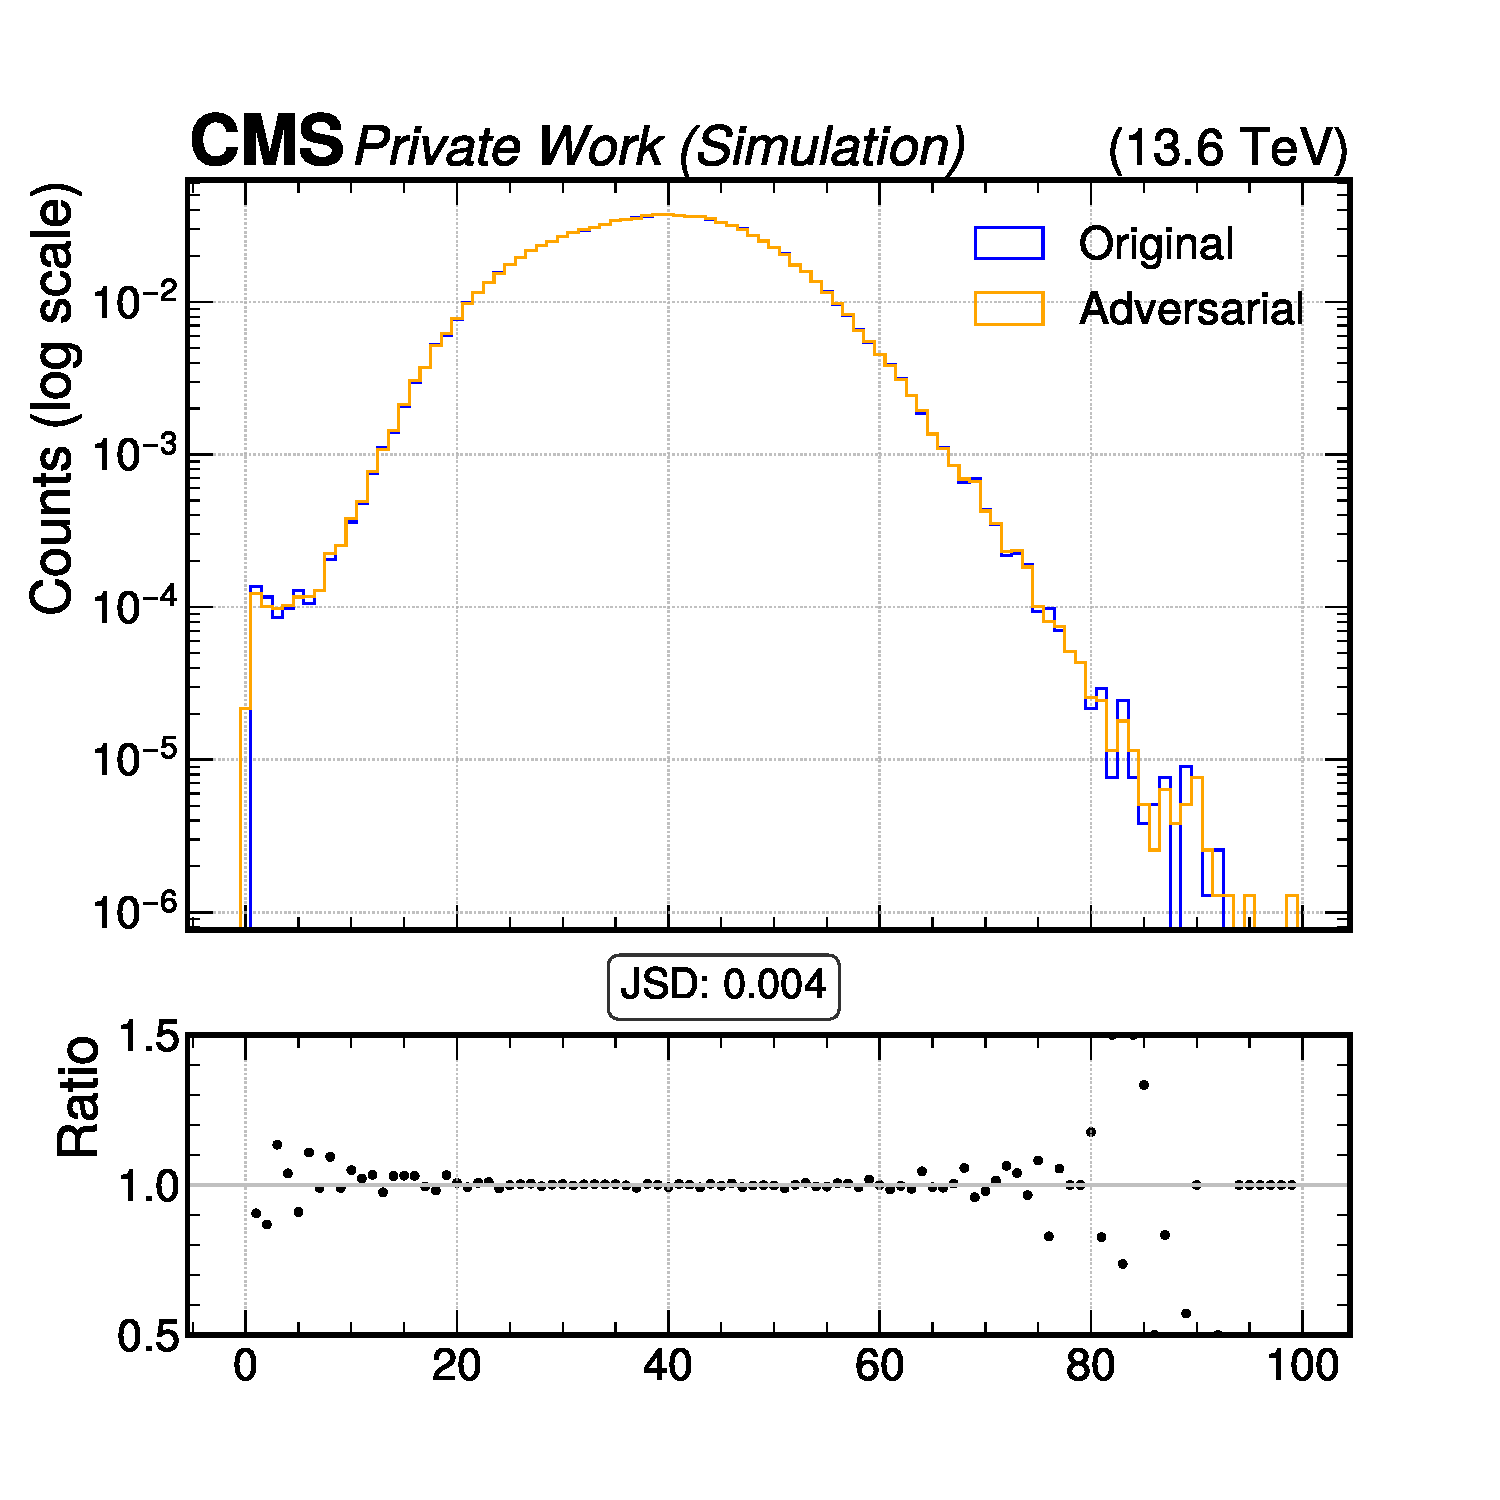
\includegraphics[width=\linewidth]{media/output/features/compare/intprob_3/cmp_global_features_npv.pdf}
    \caption{Input similarity for PIP(3).}
  \end{subfigure}

  \caption{Histogram for \texttt{npv} for multiple iterations of PIP tested against nominal inputs.}
  \label{fig:intprob_input_npv}
\end{figure}
\begin{figure}[h]
  \centering
  \begin{subfigure}[t]{0.32\textwidth}
    \includegraphics[width=\linewidth]{media/output/features/compare/intprob_1/cmp_global_features_nsv.pdf}
    \caption{Input similarity for PIP(1).}
  \end{subfigure}\hfill
  \begin{subfigure}[t]{0.32\textwidth}
    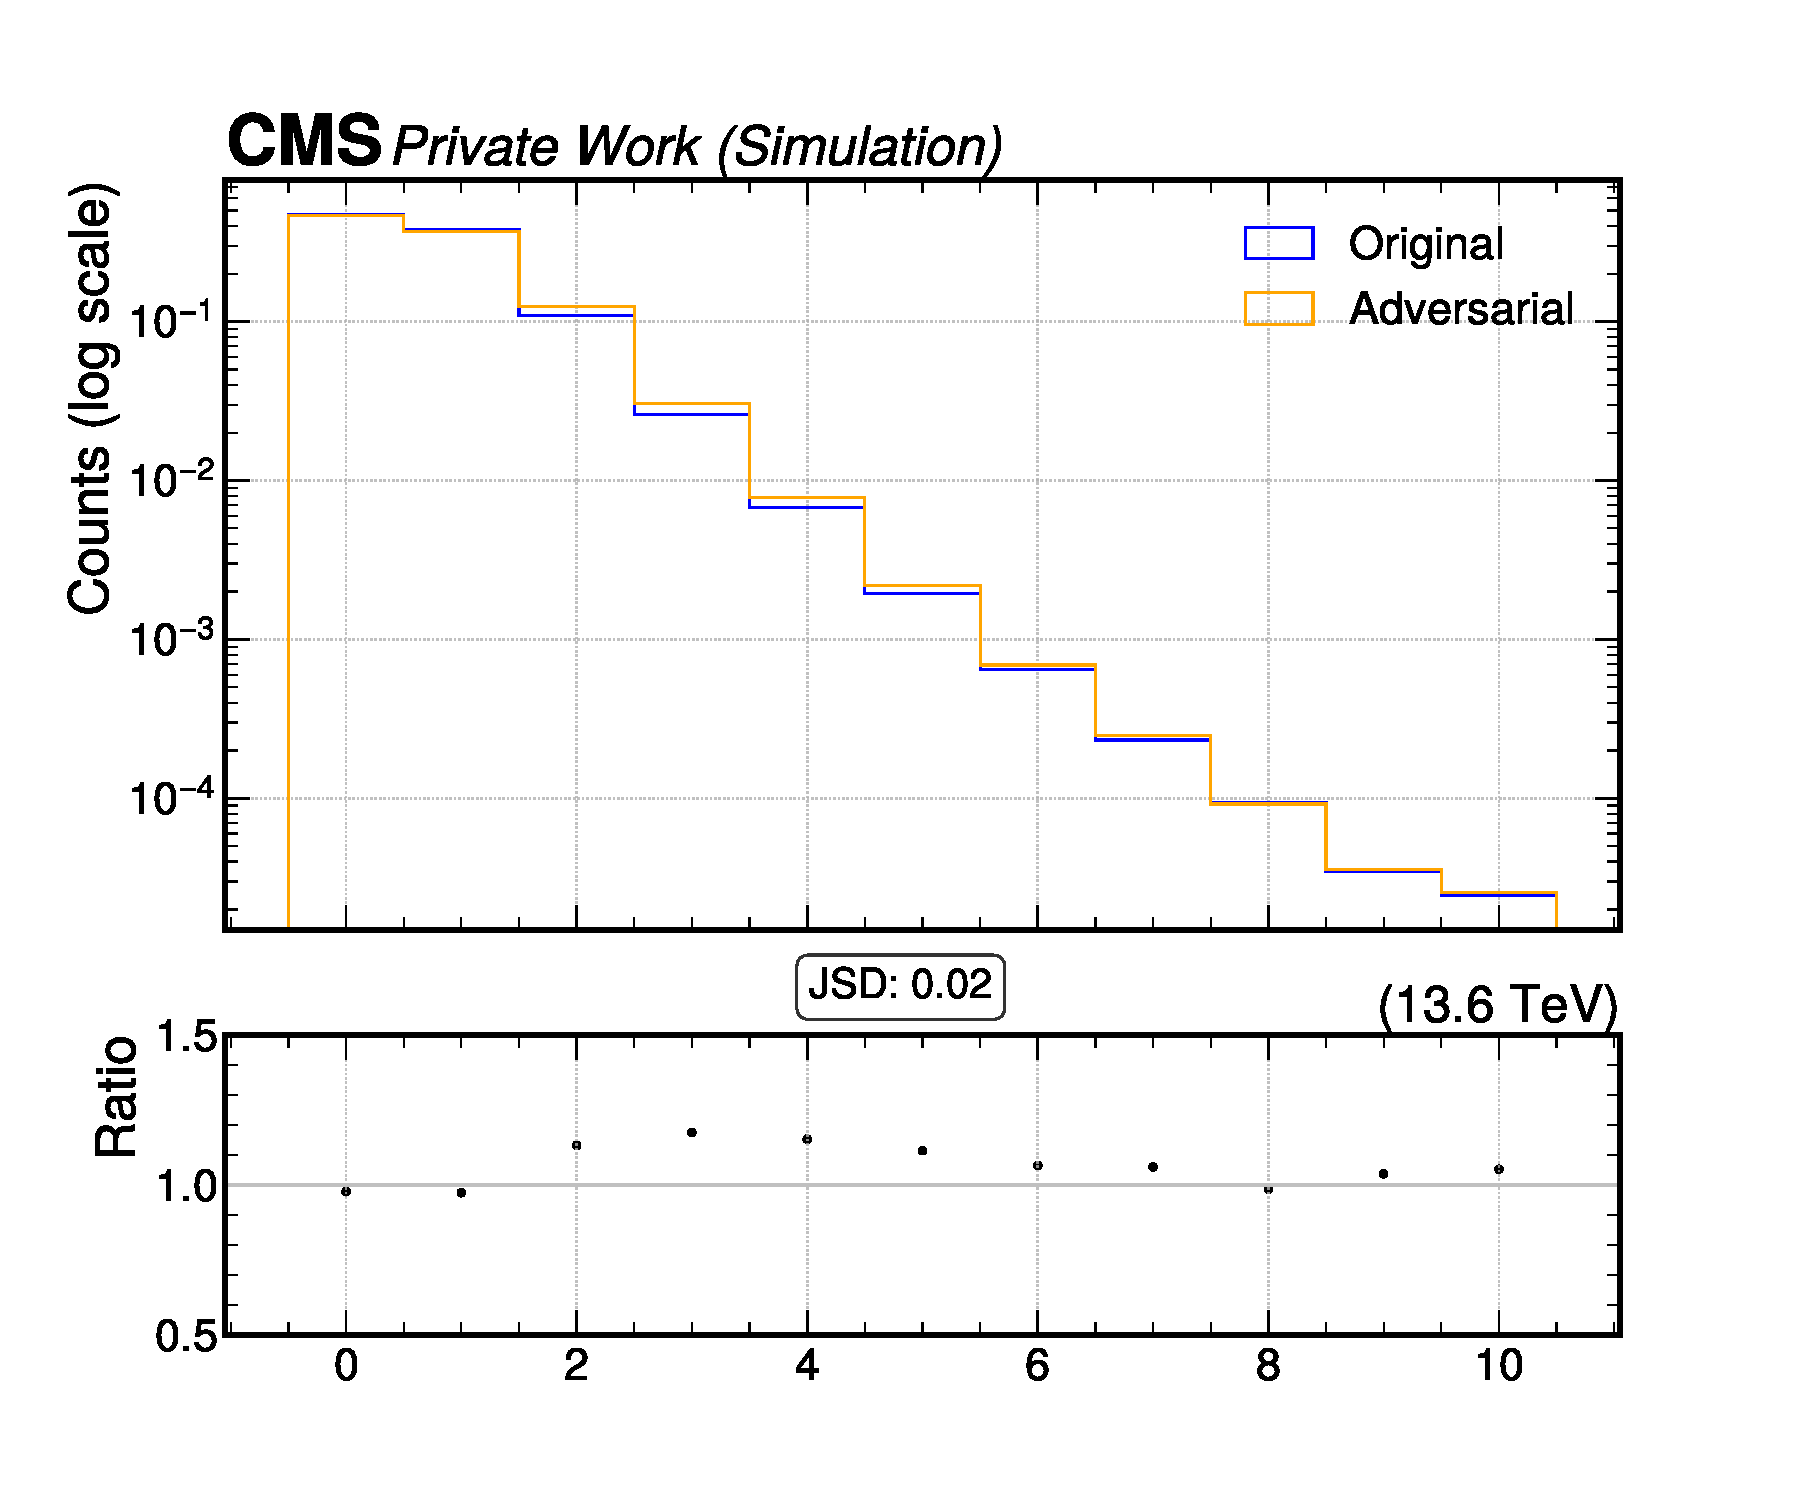
\includegraphics[width=\linewidth]{media/output/features/compare/intprob_2/cmp_global_features_nsv.pdf}
    \caption{Input similarity for PIP(2).}
  \end{subfigure}\hfill
  \begin{subfigure}[t]{0.32\textwidth}
    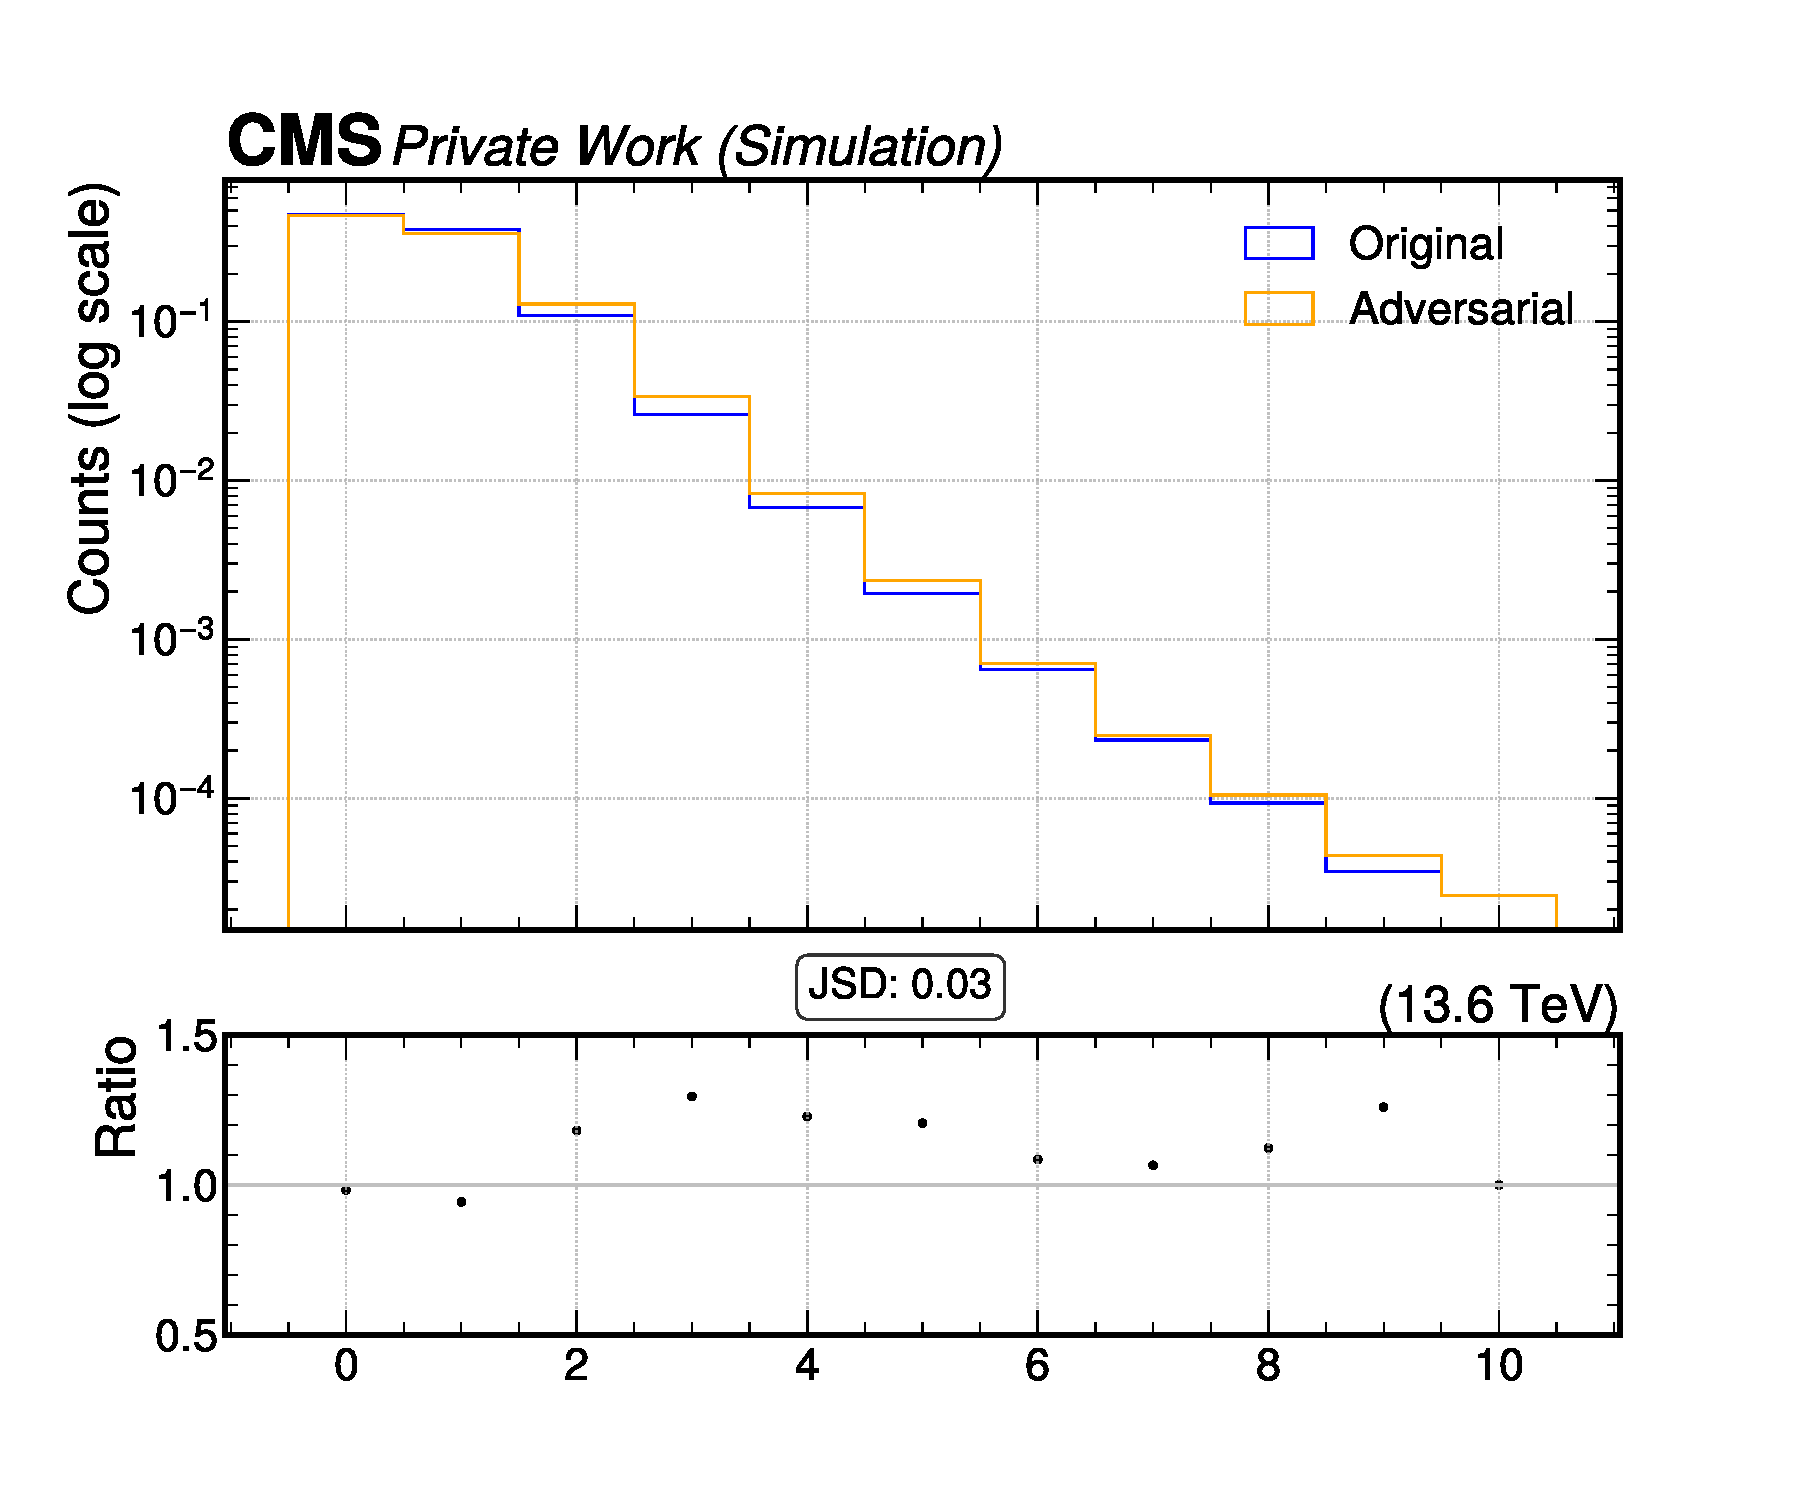
\includegraphics[width=\linewidth]{media/output/features/compare/intprob_3/cmp_global_features_nsv.pdf}
    \caption{Input similarity for PIP(3).}
  \end{subfigure}

  \caption{Histogram for \texttt{nsv} for multiple iterations of PIP tested against nominal inputs.}
  \label{fig:intprob_input_nsv}
\end{figure}
\begin{figure}[h]
  \centering
  \begin{subfigure}[t]{0.32\textwidth}
    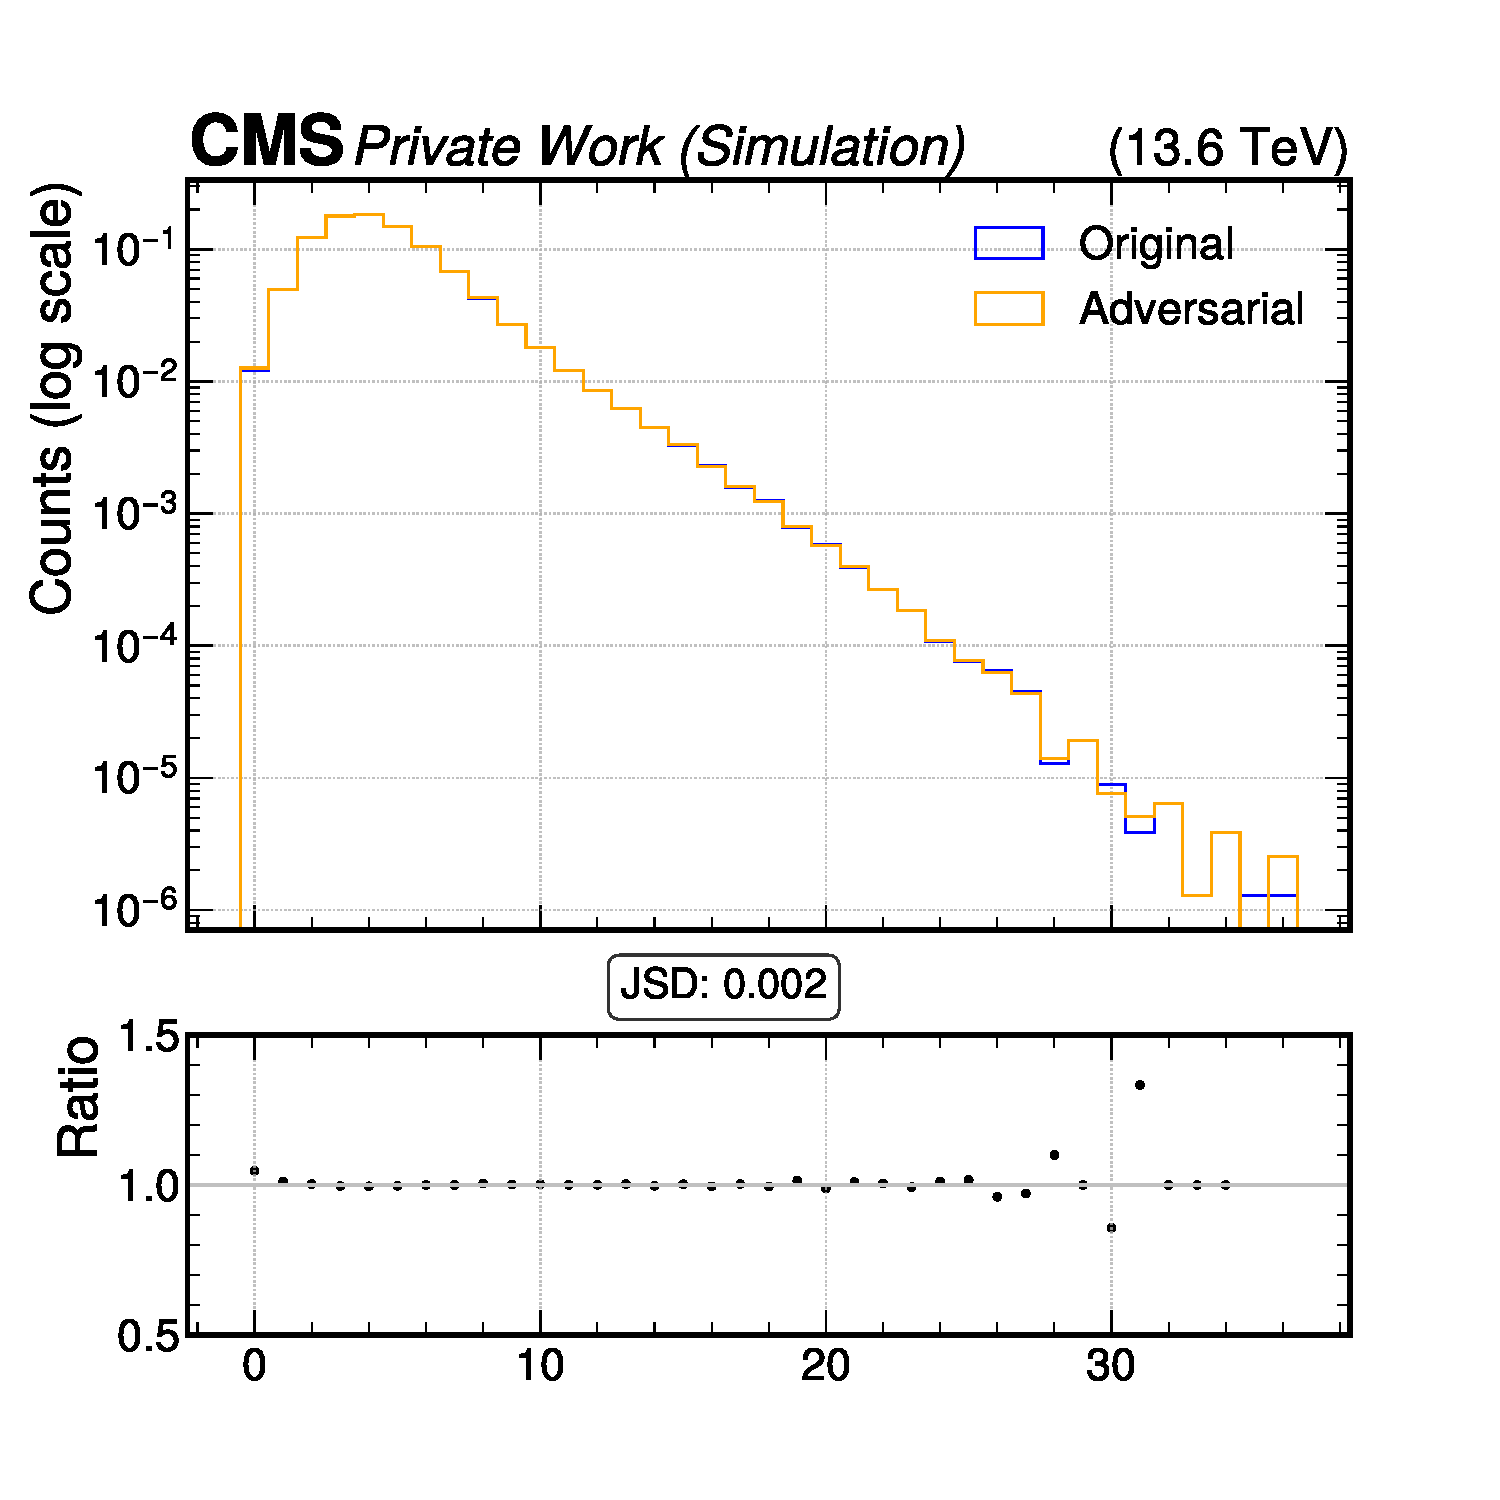
\includegraphics[width=\linewidth]{media/output/features/compare/intprob_1/cmp_global_features_TagVarCSV_jetNSelectedTracks.pdf}
    \caption{Input similarity for PIP(1).}
  \end{subfigure}\hfill
  \begin{subfigure}[t]{0.32\textwidth}
    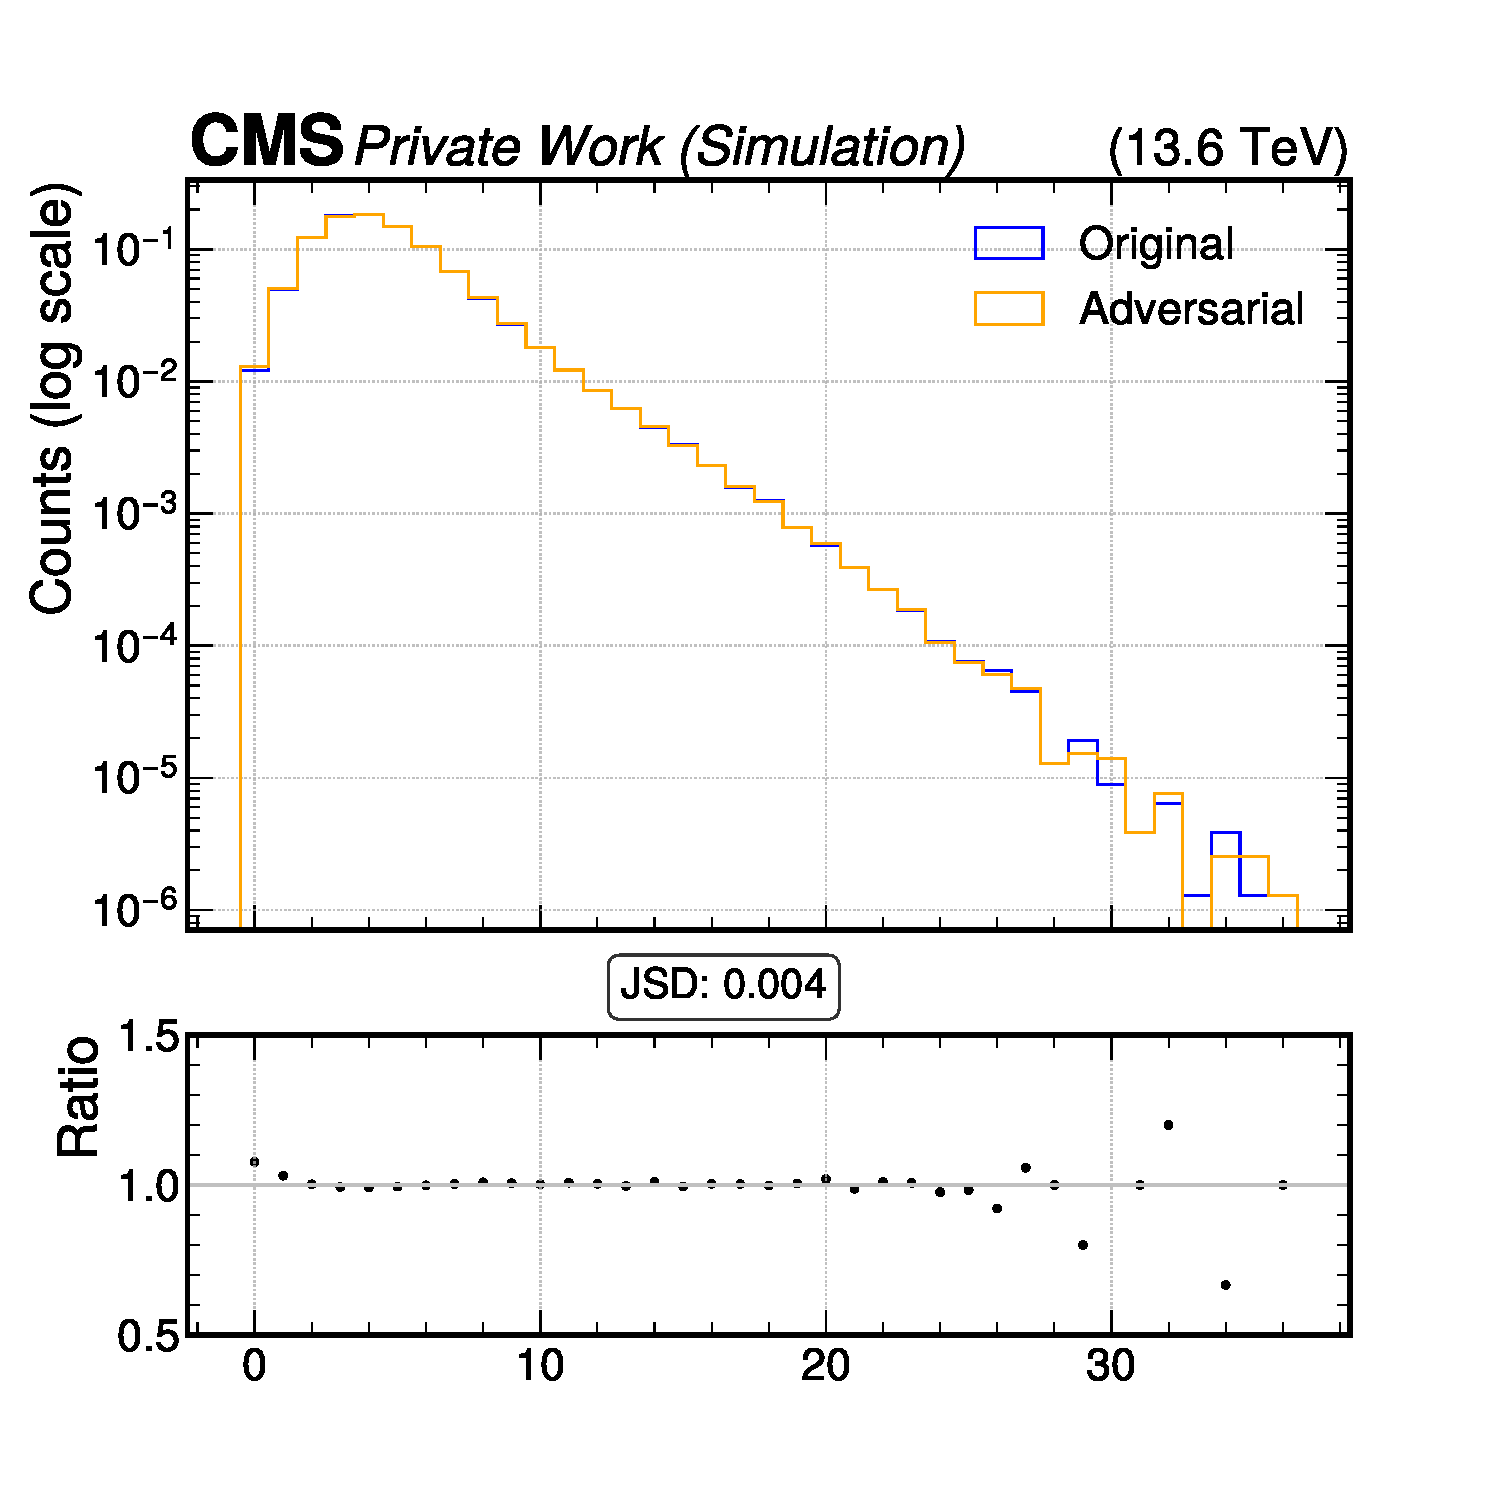
\includegraphics[width=\linewidth]{media/output/features/compare/intprob_2/cmp_global_features_TagVarCSV_jetNSelectedTracks.pdf}
    \caption{Input similarity for PIP(2).}
  \end{subfigure}\hfill
  \begin{subfigure}[t]{0.32\textwidth}
    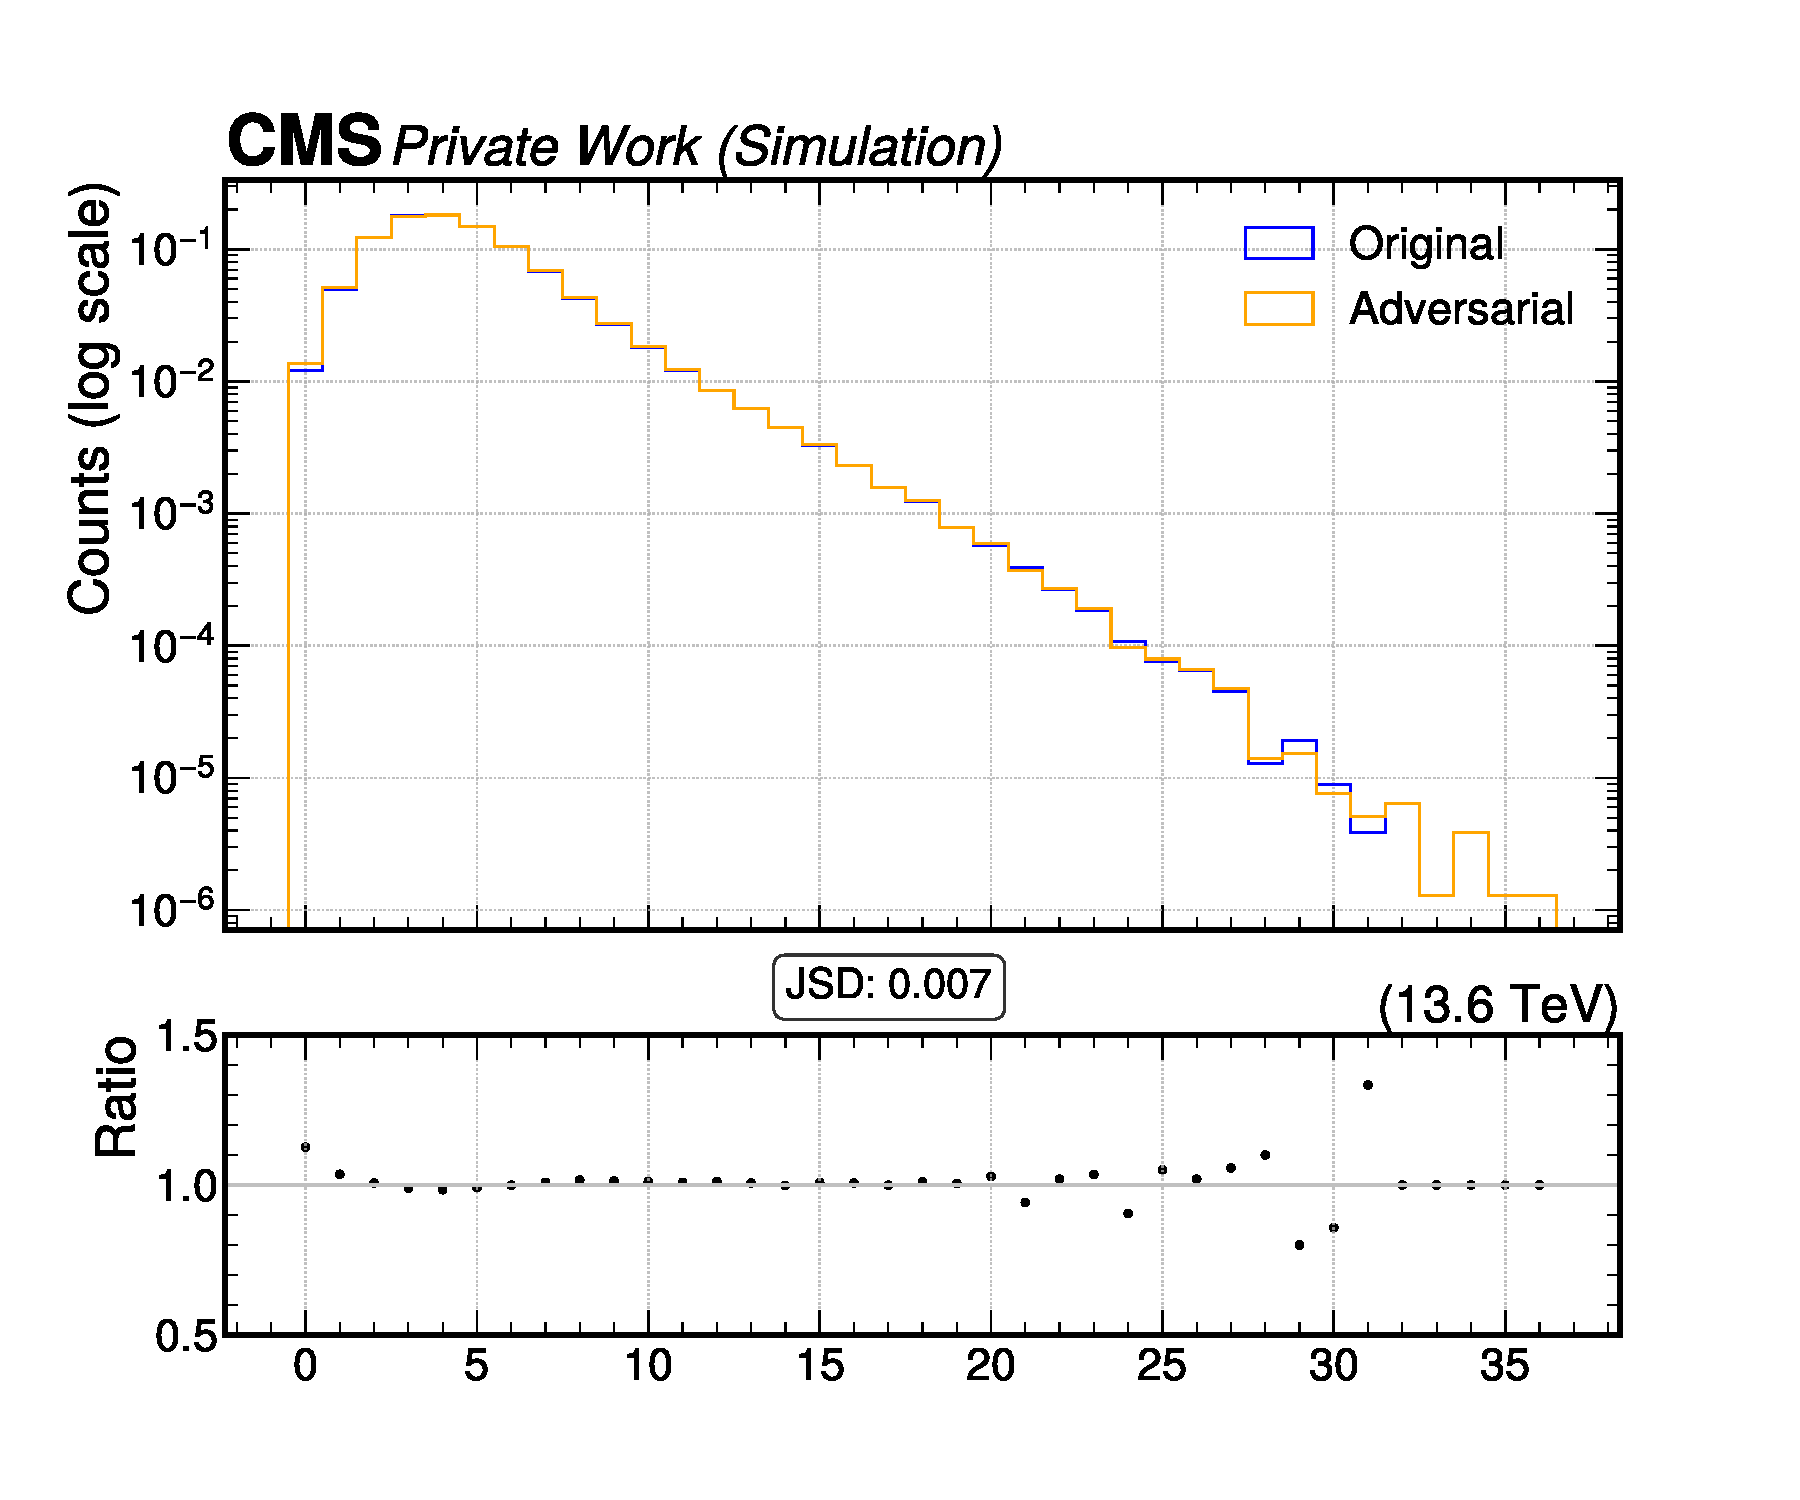
\includegraphics[width=\linewidth]{media/output/features/compare/intprob_3/cmp_global_features_TagVarCSV_jetNSelectedTracks.pdf}
    \caption{Input similarity for PIP(3).}
  \end{subfigure}

  \caption{Histogram for \texttt{TagVarCSV\_jetNSelectedTracks} for multiple iterations of PIP tested against nominal inputs.}
  \label{fig:intprob_input_TagVarCSV_jetNSelectedTracks}
\end{figure}
\begin{figure}[h]
  \centering
  \begin{subfigure}[t]{0.32\textwidth}
    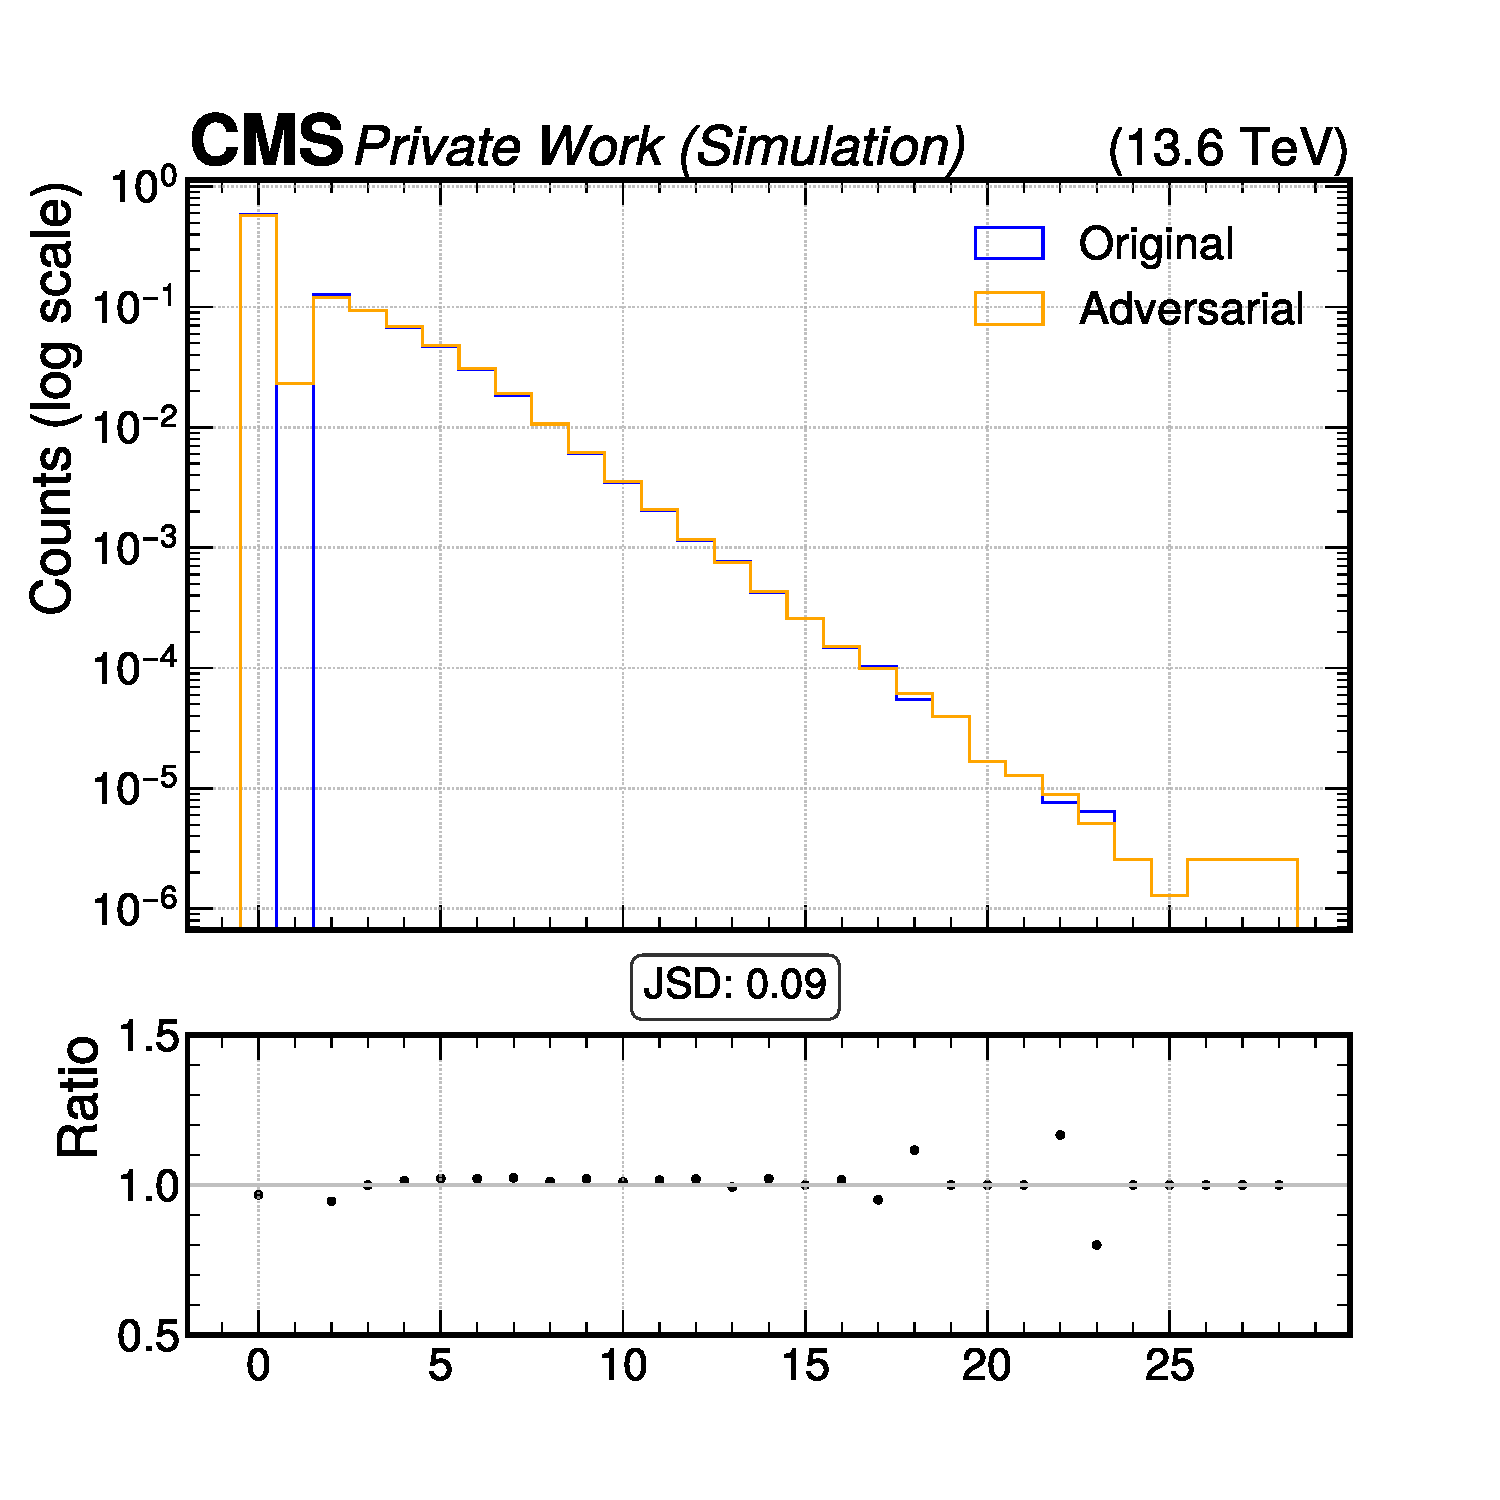
\includegraphics[width=\linewidth]{media/output/features/compare/intprob_1/cmp_global_features_TagVarCSV_jetNTracksEtaRel.pdf}
    \caption{Input similarity for PIP(1).}
  \end{subfigure}\hfill
  \begin{subfigure}[t]{0.32\textwidth}
    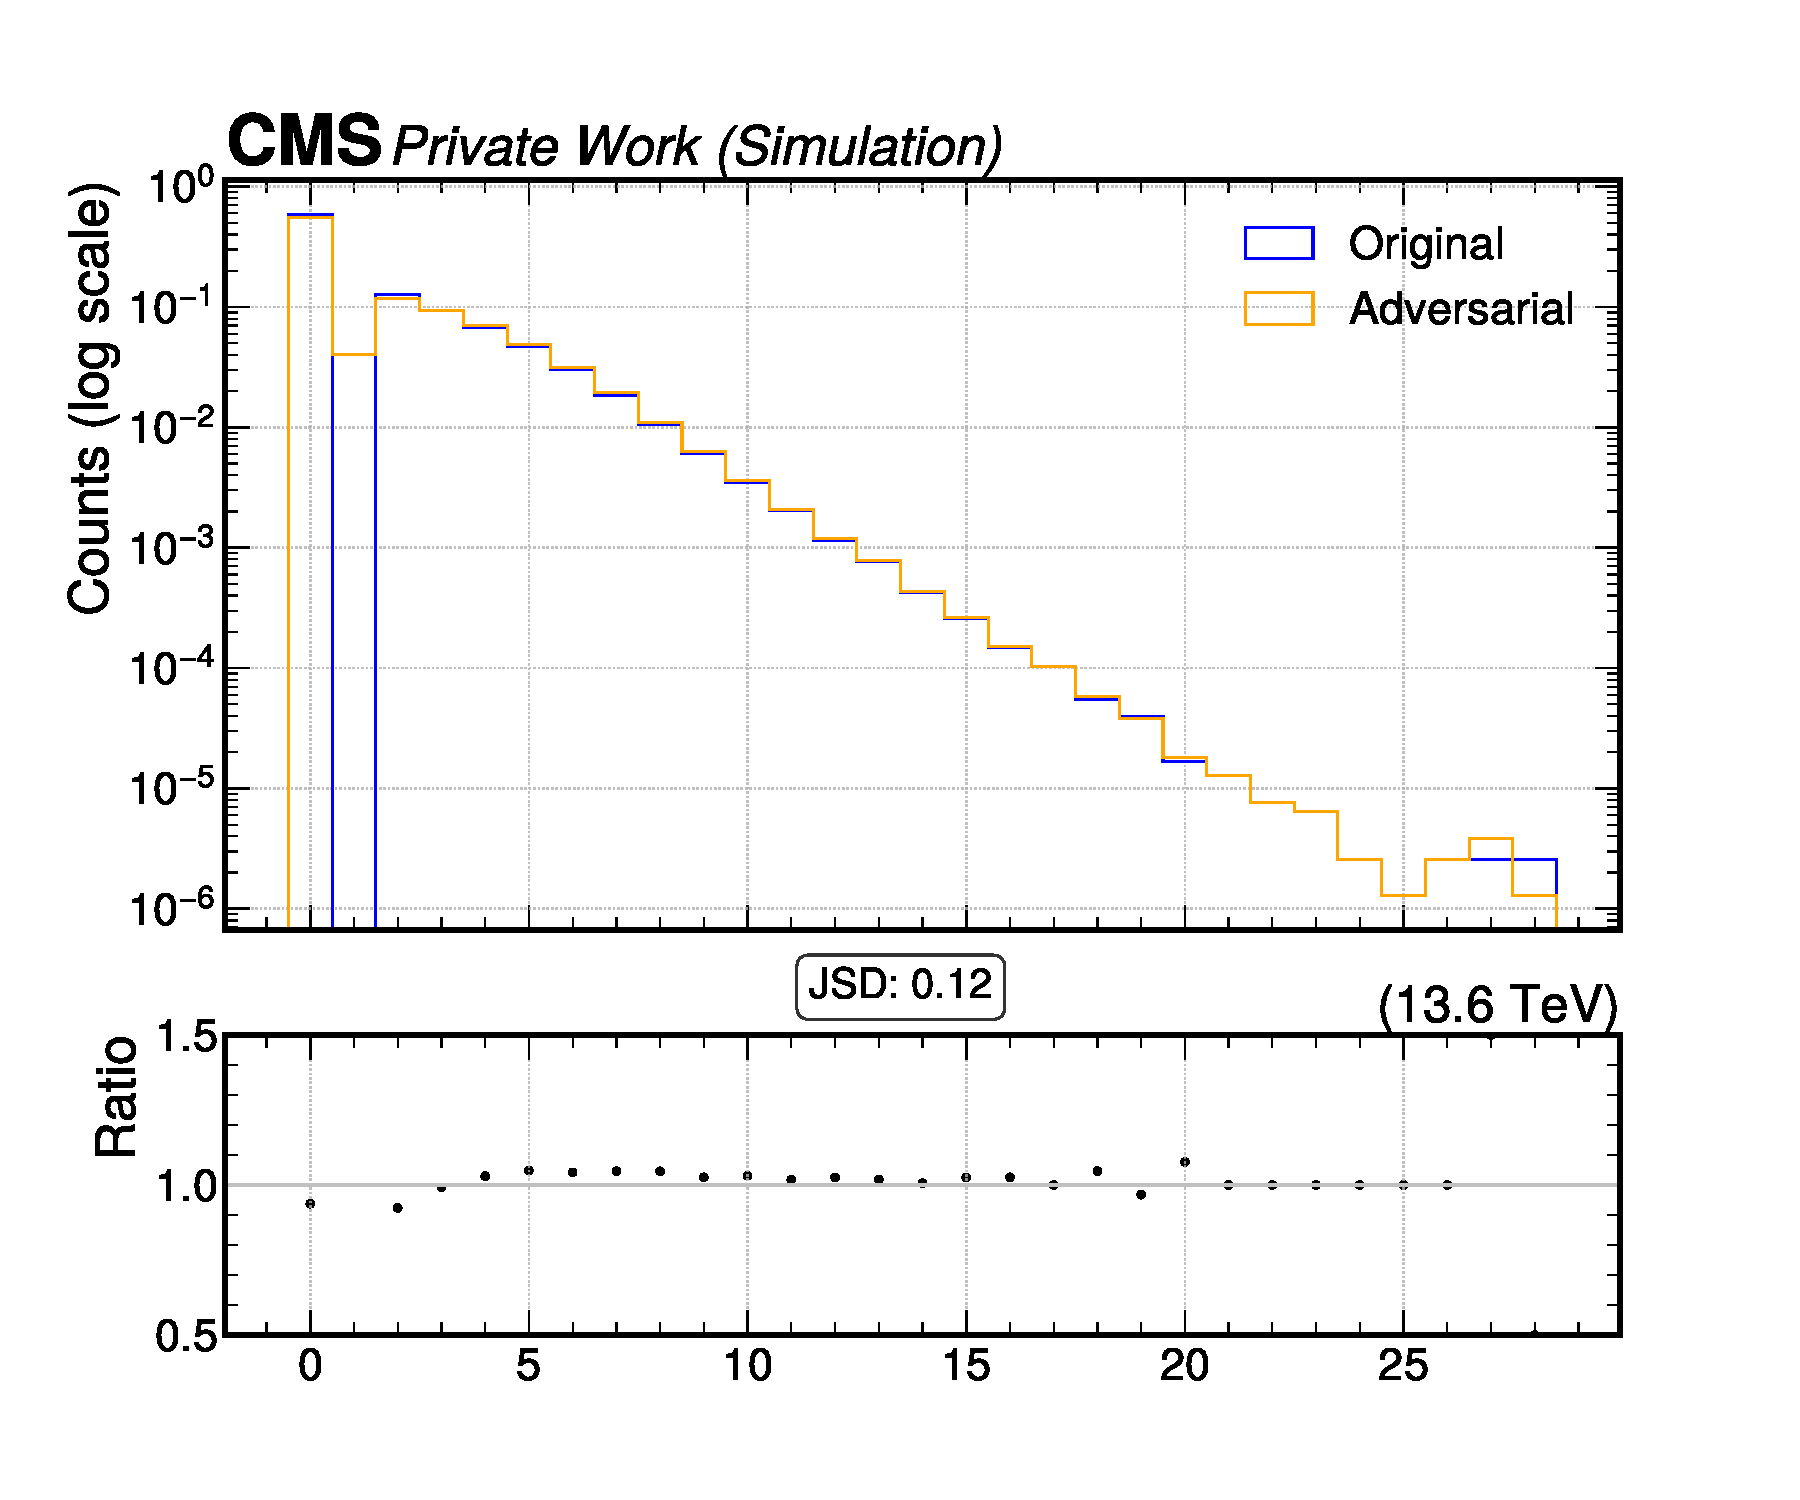
\includegraphics[width=\linewidth]{media/output/features/compare/intprob_2/cmp_global_features_TagVarCSV_jetNTracksEtaRel.pdf}
    \caption{Input similarity for PIP(2).}
  \end{subfigure}\hfill
  \begin{subfigure}[t]{0.32\textwidth}
    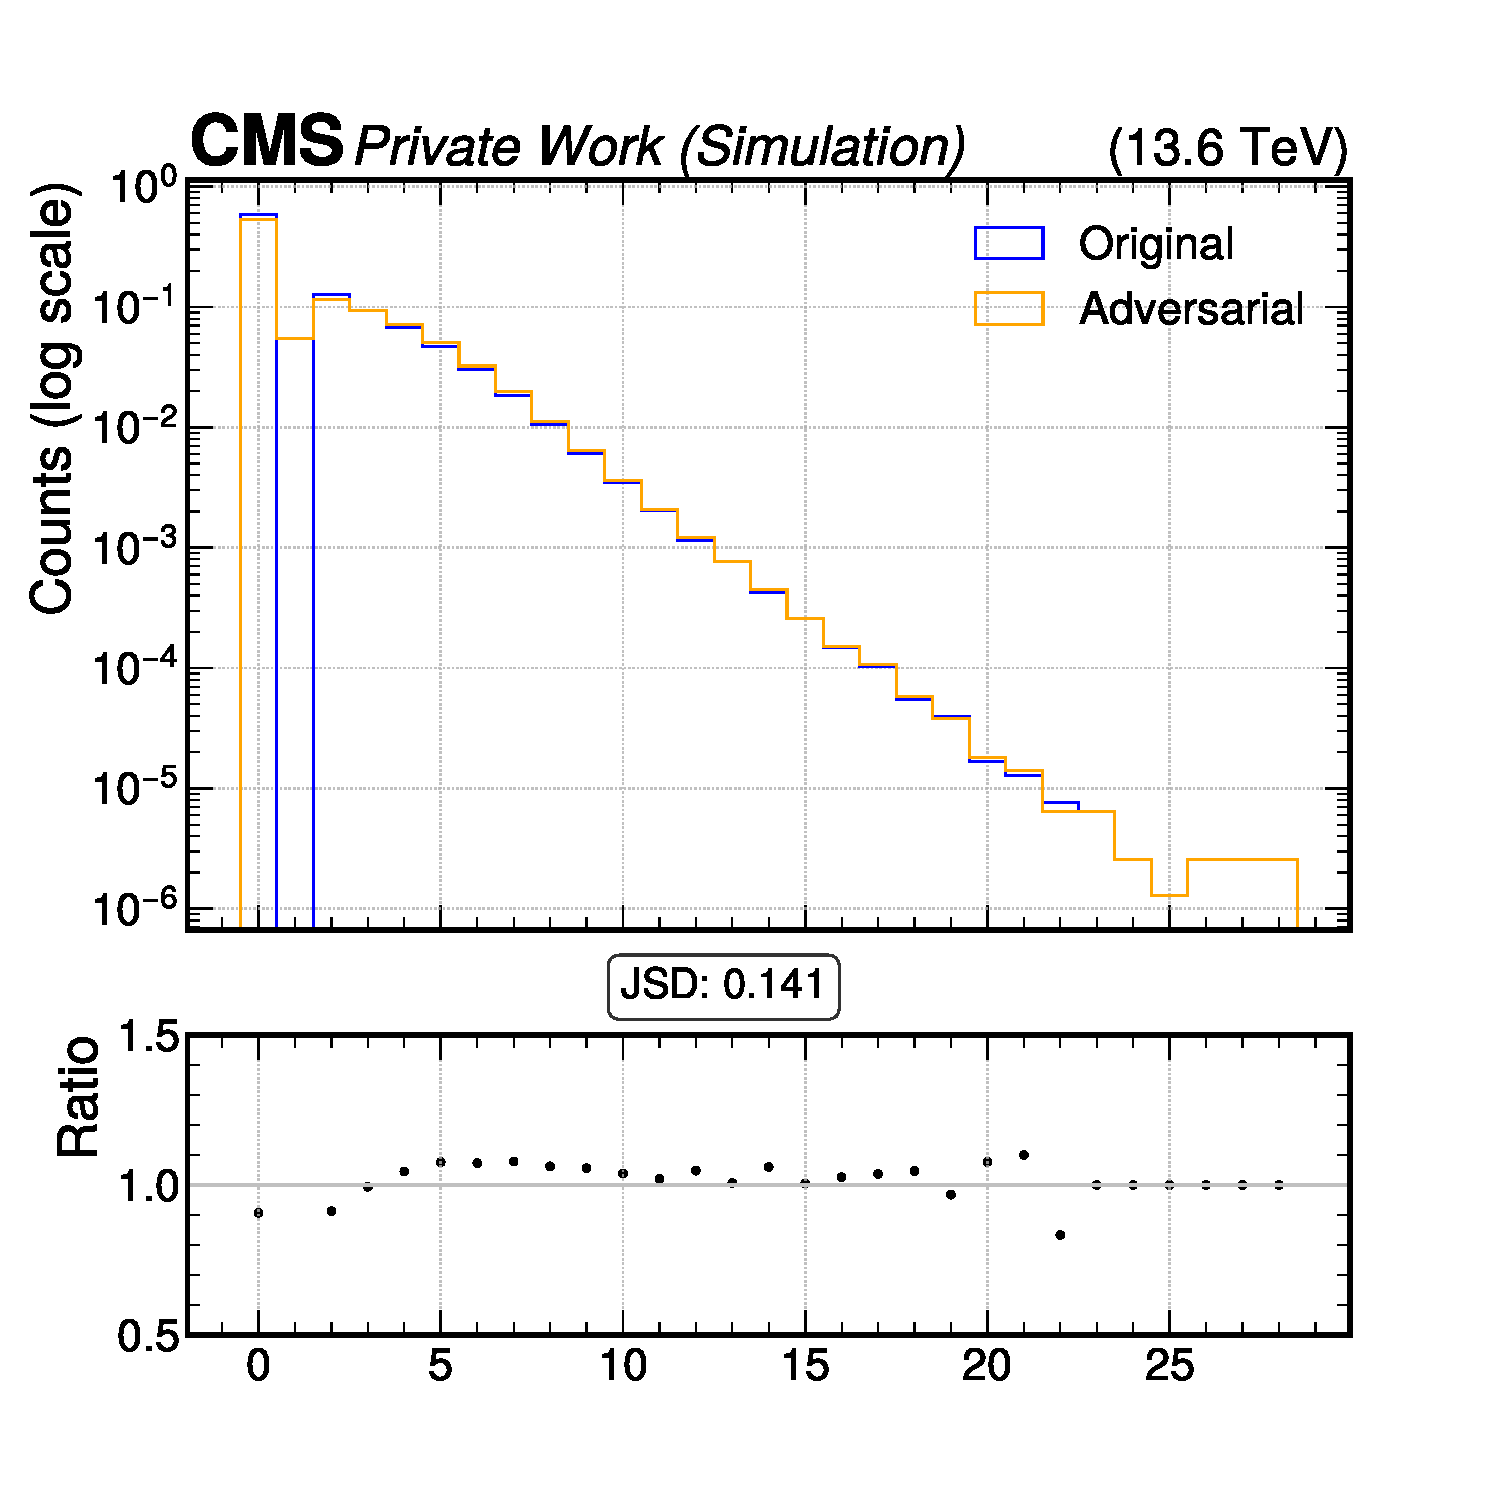
\includegraphics[width=\linewidth]{media/output/features/compare/intprob_3/cmp_global_features_TagVarCSV_jetNTracksEtaRel.pdf}
    \caption{Input similarity for PIP(3).}
  \end{subfigure}

  \caption{Histogram for \texttt{TagVarCSV\_jetNTracksEtaRel} for multiple iterations of PIP tested against nominal inputs.}
  \label{fig:intprob_input_TagVarCSV_jetNTracksEtaRel}
\end{figure}
\begin{figure}[h]
  \centering
  \begin{subfigure}[t]{0.32\textwidth}
    \includegraphics[width=\linewidth]{media/output/features/compare/intprob_1/cmp_global_features_TagVarCSV_vertexCategory.pdf}
    \caption{Input similarity for PIP(1).}
  \end{subfigure}\hfill
  \begin{subfigure}[t]{0.32\textwidth}
    \includegraphics[width=\linewidth]{media/output/features/compare/intprob_2/cmp_global_features_TagVarCSV_vertexCategory.pdf}
    \caption{Input similarity for PIP(2).}
  \end{subfigure}\hfill
  \begin{subfigure}[t]{0.32\textwidth}
    \includegraphics[width=\linewidth]{media/output/features/compare/intprob_3/cmp_global_features_TagVarCSV_vertexCategory.pdf}
    \caption{Input similarity for PIP(3).}
  \end{subfigure}

  \caption{Histogram for \texttt{TagVarCSV\_vertexCategory} for multiple iterations of PIP tested against nominal inputs.}
  \label{fig:intprob_input_TagVarCSV_vertexCategory}
\end{figure}

\FloatBarrier
\newpage
\subsection*{CPF Features}

\begin{figure}[h]
  \centering
  \begin{subfigure}[t]{0.32\textwidth}
    \includegraphics[width=\linewidth]{media/output/features/compare/intprob_1/cmp_cpf_arr_Cpfcan_quality.pdf}
    \caption{Input similarity for PIP(1).}
  \end{subfigure}\hfill
  \begin{subfigure}[t]{0.32\textwidth}
    \includegraphics[width=\linewidth]{media/output/features/compare/intprob_2/cmp_cpf_arr_Cpfcan_quality.pdf}
    \caption{Input similarity for PIP(2).}
  \end{subfigure}\hfill
  \begin{subfigure}[t]{0.32\textwidth}
    \includegraphics[width=\linewidth]{media/output/features/compare/intprob_3/cmp_cpf_arr_Cpfcan_quality.pdf}
    \caption{Input similarity for PIP(3).}
  \end{subfigure}

  \caption{Histogram for \texttt{Cpfcan\_quality} for multiple iterations of PIP tested against nominal inputs.}
  \label{fig:intprob_input_Cpfcan_quality}
\end{figure}
\begin{figure}[h]
  \centering
  \begin{subfigure}[t]{0.32\textwidth}
    \includegraphics[width=\linewidth]{media/output/features/compare/intprob_1/cmp_cpf_arr_Cpfcan_VTX_ass.pdf}
    \caption{Input similarity for PIP(1).}
  \end{subfigure}\hfill
  \begin{subfigure}[t]{0.32\textwidth}
    \includegraphics[width=\linewidth]{media/output/features/compare/intprob_2/cmp_cpf_arr_Cpfcan_VTX_ass.pdf}
    \caption{Input similarity for PIP(2).}
  \end{subfigure}\hfill
  \begin{subfigure}[t]{0.32\textwidth}
    \includegraphics[width=\linewidth]{media/output/features/compare/intprob_3/cmp_cpf_arr_Cpfcan_VTX_ass.pdf}
    \caption{Input similarity for PIP(3).}
  \end{subfigure}

  \caption{Histogram for \texttt{Cpfcan\_VTX\_ass} for multiple iterations of PIP tested against nominal inputs.}
  \label{fig:intprob_input_Cpfcan_VTX_ass}
\end{figure}

\newpage
\subsection*{NPF Features}

\begin{figure}[h]
  \centering
  \begin{subfigure}[t]{0.32\textwidth}
    \includegraphics[width=\linewidth]{media/output/features/compare/intprob_1/cmp_npf_arr_Npfcan_HadFrac.pdf}
    \caption{Input similarity for PIP(1).}
  \end{subfigure}\hfill
  \begin{subfigure}[t]{0.32\textwidth}
    \includegraphics[width=\linewidth]{media/output/features/compare/intprob_2/cmp_npf_arr_Npfcan_HadFrac.pdf}
    \caption{Input similarity for PIP(2).}
  \end{subfigure}\hfill
  \begin{subfigure}[t]{0.32\textwidth}
    \includegraphics[width=\linewidth]{media/output/features/compare/intprob_3/cmp_npf_arr_Npfcan_HadFrac.pdf}
    \caption{Input similarity for PIP(3).}
  \end{subfigure}

  \caption{Histogram for \texttt{Npfcan\_HadFrac} for multiple iterations of PIP tested against nominal inputs.}
  \label{fig:intprob_input_Npfcan_HadFrac}
\end{figure}
\begin{figure}[h]
  \centering
  \begin{subfigure}[t]{0.32\textwidth}
    \includegraphics[width=\linewidth]{media/output/features/compare/intprob_1/cmp_npf_arr_Npfcan_isGamma.pdf}
    \caption{Input similarity for PIP(1).}
  \end{subfigure}\hfill
  \begin{subfigure}[t]{0.32\textwidth}
    \includegraphics[width=\linewidth]{media/output/features/compare/intprob_2/cmp_npf_arr_Npfcan_isGamma.pdf}
    \caption{Input similarity for PIP(2).}
  \end{subfigure}\hfill
  \begin{subfigure}[t]{0.32\textwidth}
    \includegraphics[width=\linewidth]{media/output/features/compare/intprob_3/cmp_npf_arr_Npfcan_isGamma.pdf}
    \caption{Input similarity for PIP(3).}
  \end{subfigure}

  \caption{Histogram for \texttt{Npfcan\_isGamma} for multiple iterations of PIP tested against nominal inputs.}
  \label{fig:intprob_input_Npfcan_isGamma}
\end{figure}

\section{PIP-PGD Input Similarities}
\label{appendix:combined}

\subsection*{Global Features}


\begin{figure}[htbp]
  \centering
  \begin{subfigure}[t]{0.32\textwidth}
    \includegraphics[width=\linewidth]{media/output/features/compare/combined_it_1/cmp_global_features_jet_eta.pdf}
    \caption*{Input similarity for PIP-PGD(1).}
  \end{subfigure}\hfill
  \begin{subfigure}[t]{0.32\textwidth}
    \includegraphics[width=\linewidth]{media/output/features/compare/combined_it_2/cmp_global_features_jet_eta.pdf}
    \caption*{Input similarity for PIP-PGD(2).}
  \end{subfigure}\hfill
  \begin{subfigure}[t]{0.32\textwidth}
    \includegraphics[width=\linewidth]{media/output/features/compare/combined_it_3/cmp_global_features_jet_eta.pdf}
    \caption*{Input similarity for PIP-PGD(3).}
  \end{subfigure}

  \caption*{Histogram of \texttt{jet\_eta} for multiple iterations of PIP-PGD tested against nominal inputs.}
  \label{fig:combined_input_jet_eta}
\end{figure}

\begin{figure}[htbp]
  \centering
  \begin{subfigure}[t]{0.32\textwidth}
    \includegraphics[width=\linewidth]{media/output/features/compare/combined_it_1/cmp_global_features_jet_pt.pdf}
    \caption*{Input similarity for PIP-PGD(1).}
  \end{subfigure}\hfill
  \begin{subfigure}[t]{0.32\textwidth}
    \includegraphics[width=\linewidth]{media/output/features/compare/combined_it_2/cmp_global_features_jet_pt.pdf}
    \caption*{Input similarity for PIP-PGD(2).}
  \end{subfigure}\hfill
  \begin{subfigure}[t]{0.32\textwidth}
    \includegraphics[width=\linewidth]{media/output/features/compare/combined_it_3/cmp_global_features_jet_pt.pdf}
    \caption*{Input similarity for PIP-PGD(3).}
  \end{subfigure}

  \caption*{Histogram of \texttt{jet\_pt} for multiple iterations of PIP-PGD tested against nominal inputs.}
  \label{fig:combined_input_jet_pt}
\end{figure}

\begin{figure}[htbp]
  \centering
  \begin{subfigure}[t]{0.32\textwidth}
    \includegraphics[width=\linewidth]{media/output/features/compare/combined_it_1/cmp_global_features_n_Cpfcand.pdf}
    \caption*{Input similarity for PIP-PGD(1).}
  \end{subfigure}\hfill
  \begin{subfigure}[t]{0.32\textwidth}
    \includegraphics[width=\linewidth]{media/output/features/compare/combined_it_2/cmp_global_features_n_Cpfcand.pdf}
    \caption*{Input similarity for PIP-PGD(2).}
  \end{subfigure}\hfill
  \begin{subfigure}[t]{0.32\textwidth}
    \includegraphics[width=\linewidth]{media/output/features/compare/combined_it_3/cmp_global_features_n_Cpfcand.pdf}
    \caption*{Input similarity for PIP-PGD(3).}
  \end{subfigure}

  \caption*{Histogram of \texttt{n\_Cpfcand} for multiple iterations of PIP-PGD tested against nominal inputs.}
  \label{fig:combined_input_n_Cpfcand}
\end{figure}

\begin{figure}[htbp]
  \centering
  \begin{subfigure}[t]{0.32\textwidth}
    \includegraphics[width=\linewidth]{media/output/features/compare/combined_it_1/cmp_global_features_n_Npfcand.pdf}
    \caption*{Input similarity for PIP-PGD(1).}
  \end{subfigure}\hfill
  \begin{subfigure}[t]{0.32\textwidth}
    \includegraphics[width=\linewidth]{media/output/features/compare/combined_it_2/cmp_global_features_n_Npfcand.pdf}
    \caption*{Input similarity for PIP-PGD(2).}
  \end{subfigure}\hfill
  \begin{subfigure}[t]{0.32\textwidth}
    \includegraphics[width=\linewidth]{media/output/features/compare/combined_it_3/cmp_global_features_n_Npfcand.pdf}
    \caption*{Input similarity for PIP-PGD(3).}
  \end{subfigure}

  \caption*{Histogram of \texttt{n\_Npfcand} for multiple iterations of PIP-PGD tested against nominal inputs.}
  \label{fig:combined_input_n_Npfcand}
\end{figure}

\begin{figure}[htbp]
  \centering
  \begin{subfigure}[t]{0.32\textwidth}
    \includegraphics[width=\linewidth]{media/output/features/compare/combined_it_1/cmp_global_features_npv.pdf}
    \caption*{Input similarity for PIP-PGD(1).}
  \end{subfigure}\hfill
  \begin{subfigure}[t]{0.32\textwidth}
    \includegraphics[width=\linewidth]{media/output/features/compare/combined_it_2/cmp_global_features_npv.pdf}
    \caption*{Input similarity for PIP-PGD(2).}
  \end{subfigure}\hfill
  \begin{subfigure}[t]{0.32\textwidth}
    \includegraphics[width=\linewidth]{media/output/features/compare/combined_it_3/cmp_global_features_npv.pdf}
    \caption*{Input similarity for PIP-PGD(3).}
  \end{subfigure}

  \caption*{Histogram of \texttt{npv} for multiple iterations of PIP-PGD tested against nominal inputs.}
  \label{fig:combined_input_npv}
\end{figure}

\begin{figure}[htbp]
  \centering
  \begin{subfigure}[t]{0.32\textwidth}
    \includegraphics[width=\linewidth]{media/output/features/compare/combined_it_1/cmp_global_features_nsv.pdf}
    \caption*{Input similarity for PIP-PGD(1).}
  \end{subfigure}\hfill
  \begin{subfigure}[t]{0.32\textwidth}
    \includegraphics[width=\linewidth]{media/output/features/compare/combined_it_2/cmp_global_features_nsv.pdf}
    \caption*{Input similarity for PIP-PGD(2).}
  \end{subfigure}\hfill
  \begin{subfigure}[t]{0.32\textwidth}
    \includegraphics[width=\linewidth]{media/output/features/compare/combined_it_3/cmp_global_features_nsv.pdf}
    \caption*{Input similarity for PIP-PGD(3).}
  \end{subfigure}

  \caption*{Histogram of \texttt{nsv} for multiple iterations of PIP-PGD tested against nominal inputs.}
  \label{fig:combined_input_nsv}
\end{figure}

\begin{figure}[htbp]
  \centering
  \begin{subfigure}[t]{0.32\textwidth}
    \includegraphics[width=\linewidth]{media/output/features/compare/combined_it_1/cmp_global_features_TagVarCSV_jetNSelectedTracks.pdf}
    \caption*{Input similarity for PIP-PGD(1).}
  \end{subfigure}\hfill
  \begin{subfigure}[t]{0.32\textwidth}
    \includegraphics[width=\linewidth]{media/output/features/compare/combined_it_2/cmp_global_features_TagVarCSV_jetNSelectedTracks.pdf}
    \caption*{Input similarity for PIP-PGD(2).}
  \end{subfigure}\hfill
  \begin{subfigure}[t]{0.32\textwidth}
    \includegraphics[width=\linewidth]{media/output/features/compare/combined_it_3/cmp_global_features_TagVarCSV_jetNSelectedTracks.pdf}
    \caption*{Input similarity for PIP-PGD(3).}
  \end{subfigure}

  \caption*{Histogram of \texttt{TagVarCSV\_jetNSelectedTracks} for multiple iterations of PIP-PGD tested against nominal inputs.}
  \label{fig:combined_input_TagVarCSV_jetNSelectedTracks}
\end{figure}

\begin{figure}[htbp]
  \centering
  \begin{subfigure}[t]{0.32\textwidth}
    \includegraphics[width=\linewidth]{media/output/features/compare/combined_it_1/cmp_global_features_TagVarCSV_jetNTracksEtaRel.pdf}
    \caption*{Input similarity for PIP-PGD(1).}
  \end{subfigure}\hfill
  \begin{subfigure}[t]{0.32\textwidth}
    \includegraphics[width=\linewidth]{media/output/features/compare/combined_it_2/cmp_global_features_TagVarCSV_jetNTracksEtaRel.pdf}
    \caption*{Input similarity for PIP-PGD(2).}
  \end{subfigure}\hfill
  \begin{subfigure}[t]{0.32\textwidth}
    \includegraphics[width=\linewidth]{media/output/features/compare/combined_it_3/cmp_global_features_TagVarCSV_jetNTracksEtaRel.pdf}
    \caption*{Input similarity for PIP-PGD(3).}
  \end{subfigure}

  \caption*{Histogram of \texttt{TagVarCSV\_jetNTracksEtaRel} for multiple iterations of PIP-PGD tested against nominal inputs.}
  \label{fig:combined_input_TagVarCSV_jetNTracksEtaRel}
\end{figure}

\begin{figure}[htbp]
  \centering
  \begin{subfigure}[t]{0.32\textwidth}
    \includegraphics[width=\linewidth]{media/output/features/compare/combined_it_1/cmp_global_features_TagVarCSV_trackSip2dSigAboveCharm.pdf}
    \caption*{Input similarity for PIP-PGD(1).}
  \end{subfigure}\hfill
  \begin{subfigure}[t]{0.32\textwidth}
    \includegraphics[width=\linewidth]{media/output/features/compare/combined_it_2/cmp_global_features_TagVarCSV_trackSip2dSigAboveCharm.pdf}
    \caption*{Input similarity for PIP-PGD(2).}
  \end{subfigure}\hfill
  \begin{subfigure}[t]{0.32\textwidth}
    \includegraphics[width=\linewidth]{media/output/features/compare/combined_it_3/cmp_global_features_TagVarCSV_trackSip2dSigAboveCharm.pdf}
    \caption*{Input similarity for PIP-PGD(3).}
  \end{subfigure}

  \caption*{Histogram of \texttt{TagVarCSV\_trackSip2dSigAboveCharm} for multiple iterations of PIP-PGD tested against nominal inputs.}
  \label{fig:combined_input_TagVarCSV_trackSip2dSigAboveCharm}
\end{figure}

\begin{figure}[htbp]
  \centering
  \begin{subfigure}[t]{0.32\textwidth}
    \includegraphics[width=\linewidth]{media/output/features/compare/combined_it_1/cmp_global_features_TagVarCSV_trackSumJetDeltaR.pdf}
    \caption*{Input similarity for PIP-PGD(1).}
  \end{subfigure}\hfill
  \begin{subfigure}[t]{0.32\textwidth}
    \includegraphics[width=\linewidth]{media/output/features/compare/combined_it_2/cmp_global_features_TagVarCSV_trackSumJetDeltaR.pdf}
    \caption*{Input similarity for PIP-PGD(2).}
  \end{subfigure}\hfill
  \begin{subfigure}[t]{0.32\textwidth}
    \includegraphics[width=\linewidth]{media/output/features/compare/combined_it_3/cmp_global_features_TagVarCSV_trackSumJetDeltaR.pdf}
    \caption*{Input similarity for PIP-PGD(3).}
  \end{subfigure}

  \caption*{Histogram of \texttt{TagVarCSV\_trackSumJetDeltaR} for multiple iterations of PIP-PGD tested against nominal inputs.}
  \label{fig:combined_input_TagVarCSV_trackSumJetDeltaR}
\end{figure}

\begin{figure}[htbp]
  \centering
  \begin{subfigure}[t]{0.32\textwidth}
    \includegraphics[width=\linewidth]{media/output/features/compare/combined_it_1/cmp_global_features_TagVarCSV_trackSip2dValAboveCharm.pdf}
    \caption*{Input similarity for PIP-PGD(1).}
  \end{subfigure}\hfill
  \begin{subfigure}[t]{0.32\textwidth}
    \includegraphics[width=\linewidth]{media/output/features/compare/combined_it_2/cmp_global_features_TagVarCSV_trackSip2dValAboveCharm.pdf}
    \caption*{Input similarity for PIP-PGD(2).}
  \end{subfigure}\hfill
  \begin{subfigure}[t]{0.32\textwidth}
    \includegraphics[width=\linewidth]{media/output/features/compare/combined_it_3/cmp_global_features_TagVarCSV_trackSip2dValAboveCharm.pdf}
    \caption*{Input similarity for PIP-PGD(3).}
  \end{subfigure}

  \caption*{Histogram of \texttt{TagVarCSV\_trackSip2dValAboveCharm} for multiple iterations of PIP-PGD tested against nominal inputs.}
  \label{fig:combined_input_TagVarCSV_trackSip2dValAboveCharm}
\end{figure}

\begin{figure}[htbp]
  \centering
  \begin{subfigure}[t]{0.32\textwidth}
    \includegraphics[width=\linewidth]{media/output/features/compare/combined_it_1/cmp_global_features_TagVarCSV_trackSip3dSigAboveCharm.pdf}
    \caption*{Input similarity for PIP-PGD(1).}
  \end{subfigure}\hfill
  \begin{subfigure}[t]{0.32\textwidth}
    \includegraphics[width=\linewidth]{media/output/features/compare/combined_it_2/cmp_global_features_TagVarCSV_trackSip3dSigAboveCharm.pdf}
    \caption*{Input similarity for PIP-PGD(2).}
  \end{subfigure}\hfill
  \begin{subfigure}[t]{0.32\textwidth}
    \includegraphics[width=\linewidth]{media/output/features/compare/combined_it_3/cmp_global_features_TagVarCSV_trackSip3dSigAboveCharm.pdf}
    \caption*{Input similarity for PIP-PGD(3).}
  \end{subfigure}

  \caption*{Histogram of \texttt{TagVarCSV\_trackSip3dSigAboveCharm} for multiple iterations of PIP-PGD tested against nominal inputs.}
  \label{fig:combined_input_TagVarCSV_trackSip3dSigAboveCharm}
\end{figure}

\begin{figure}[htbp]
  \centering
  \begin{subfigure}[t]{0.32\textwidth}
    \includegraphics[width=\linewidth]{media/output/features/compare/combined_it_1/cmp_global_features_TagVarCSV_trackSip3dValAboveCharm.pdf}
    \caption*{Input similarity for PIP-PGD(1).}
  \end{subfigure}\hfill
  \begin{subfigure}[t]{0.32\textwidth}
    \includegraphics[width=\linewidth]{media/output/features/compare/combined_it_2/cmp_global_features_TagVarCSV_trackSip3dValAboveCharm.pdf}
    \caption*{Input similarity for PIP-PGD(2).}
  \end{subfigure}\hfill
  \begin{subfigure}[t]{0.32\textwidth}
    \includegraphics[width=\linewidth]{media/output/features/compare/combined_it_3/cmp_global_features_TagVarCSV_trackSip3dValAboveCharm.pdf}
    \caption*{Input similarity for PIP-PGD(3).}
  \end{subfigure}

  \caption*{Histogram of \texttt{TagVarCSV\_trackSip3dValAboveCharm} for multiple iterations of PIP-PGD tested against nominal inputs.}
  \label{fig:combined_input_TagVarCSV_trackSip3dValAboveCharm}
\end{figure}

\begin{figure}[htbp]
  \centering
  \begin{subfigure}[t]{0.32\textwidth}
    \includegraphics[width=\linewidth]{media/output/features/compare/combined_it_1/cmp_global_features_TagVarCSV_trackSumJetDeltaR.pdf}
    \caption*{Input similarity for PIP-PGD(1).}
  \end{subfigure}\hfill
  \begin{subfigure}[t]{0.32\textwidth}
    \includegraphics[width=\linewidth]{media/output/features/compare/combined_it_2/cmp_global_features_TagVarCSV_trackSumJetDeltaR.pdf}
    \caption*{Input similarity for PIP-PGD(2).}
  \end{subfigure}\hfill
  \begin{subfigure}[t]{0.32\textwidth}
    \includegraphics[width=\linewidth]{media/output/features/compare/combined_it_3/cmp_global_features_TagVarCSV_trackSumJetDeltaR.pdf}
    \caption*{Input similarity for PIP-PGD(3).}
  \end{subfigure}

  \caption*{Histogram of \texttt{TagVarCSV\_trackSumJetDeltaR} for multiple iterations of PIP-PGD tested against nominal inputs.}
  \label{fig:combined_input_TagVarCSV_trackSumJetDeltaR}
\end{figure}

\begin{figure}[htbp]
  \centering
  \begin{subfigure}[t]{0.32\textwidth}
    \includegraphics[width=\linewidth]{media/output/features/compare/combined_it_1/cmp_global_features_TagVarCSV_trackSumJetEtRatio.pdf}
    \caption*{Input similarity for PIP-PGD(1).}
  \end{subfigure}\hfill
  \begin{subfigure}[t]{0.32\textwidth}
    \includegraphics[width=\linewidth]{media/output/features/compare/combined_it_2/cmp_global_features_TagVarCSV_trackSumJetEtRatio.pdf}
    \caption*{Input similarity for PIP-PGD(2).}
  \end{subfigure}\hfill
  \begin{subfigure}[t]{0.32\textwidth}
    \includegraphics[width=\linewidth]{media/output/features/compare/combined_it_3/cmp_global_features_TagVarCSV_trackSumJetEtRatio.pdf}
    \caption*{Input similarity for PIP-PGD(3).}
  \end{subfigure}

  \caption*{Histogram of \texttt{TagVarCSV\_trackSumJetEtRatio} for multiple iterations of PIP-PGD tested against nominal inputs.}
  \label{fig:combined_input_TagVarCSV_trackSumJetEtRatio}
\end{figure}

\begin{figure}[htbp]
  \centering
  \begin{subfigure}[t]{0.32\textwidth}
    \includegraphics[width=\linewidth]{media/output/features/compare/combined_it_1/cmp_global_features_TagVarCSV_vertexCategory.pdf}
    \caption*{Input similarity for PIP-PGD(1).}
  \end{subfigure}\hfill
  \begin{subfigure}[t]{0.32\textwidth}
    \includegraphics[width=\linewidth]{media/output/features/compare/combined_it_2/cmp_global_features_TagVarCSV_vertexCategory.pdf}
    \caption*{Input similarity for PIP-PGD(2).}
  \end{subfigure}\hfill
  \begin{subfigure}[t]{0.32\textwidth}
    \includegraphics[width=\linewidth]{media/output/features/compare/combined_it_3/cmp_global_features_TagVarCSV_vertexCategory.pdf}
    \caption*{Input similarity for PIP-PGD(3).}
  \end{subfigure}

  \caption*{Histogram of \texttt{TagVarCSV\_vertexCategory} for multiple iterations of PIP-PGD tested against nominal inputs.}
  \label{fig:combined_input_TagVarCSV_vertexCategory}
\end{figure}

\newpage
\subsection*{CPF Features}


\begin{figure}[htbp]
  \centering
  \begin{subfigure}[t]{0.32\textwidth}
    \includegraphics[width=\linewidth]{media/output/features/compare/combined_it_1/cmp_cpf_arr_Cpfcan_chi2.pdf}
    \caption*{Input similarity for PIP-PGD(1).}
  \end{subfigure}\hfill
  \begin{subfigure}[t]{0.32\textwidth}
    \includegraphics[width=\linewidth]{media/output/features/compare/combined_it_2/cmp_cpf_arr_Cpfcan_chi2.pdf}
    \caption*{Input similarity for PIP-PGD(2).}
  \end{subfigure}\hfill
  \begin{subfigure}[t]{0.32\textwidth}
    \includegraphics[width=\linewidth]{media/output/features/compare/combined_it_3/cmp_cpf_arr_Cpfcan_chi2.pdf}
    \caption*{Input similarity for PIP-PGD(3).}
  \end{subfigure}

  \caption*{Histogram of \texttt{Cpfcan\_chi2} for multiple iterations of PIP-PGD tested against nominal inputs.}
  \label{fig:combined_input_Cpfcan_chi2}
\end{figure}

\begin{figure}[htbp]
  \centering
  \begin{subfigure}[t]{0.32\textwidth}
    \includegraphics[width=\linewidth]{media/output/features/compare/combined_it_1/cmp_cpf_arr_Cpfcan_chi2.pdf}
    \caption*{Input similarity for PIP-PGD(1).}
  \end{subfigure}\hfill
  \begin{subfigure}[t]{0.32\textwidth}
    \includegraphics[width=\linewidth]{media/output/features/compare/combined_it_2/cmp_cpf_arr_Cpfcan_chi2.pdf}
    \caption*{Input similarity for PIP-PGD(2).}
  \end{subfigure}\hfill
  \begin{subfigure}[t]{0.32\textwidth}
    \includegraphics[width=\linewidth]{media/output/features/compare/combined_it_3/cmp_cpf_arr_Cpfcan_chi2.pdf}
    \caption*{Input similarity for PIP-PGD(3).}
  \end{subfigure}

  \caption*{Histogram of \texttt{Cpfcan\_chi2} for multiple iterations of PIP-PGD tested against nominal inputs.}
  \label{fig:combined_input_Cpfcan_chi2}
\end{figure}

\begin{figure}[htbp]
  \centering
  \begin{subfigure}[t]{0.32\textwidth}
    \includegraphics[width=\linewidth]{media/output/features/compare/combined_it_1/cmp_cpf_arr_Cpfcan_drminsv.pdf}
    \caption*{Input similarity for PIP-PGD(1).}
  \end{subfigure}\hfill
  \begin{subfigure}[t]{0.32\textwidth}
    \includegraphics[width=\linewidth]{media/output/features/compare/combined_it_2/cmp_cpf_arr_Cpfcan_drminsv.pdf}
    \caption*{Input similarity for PIP-PGD(2).}
  \end{subfigure}\hfill
  \begin{subfigure}[t]{0.32\textwidth}
    \includegraphics[width=\linewidth]{media/output/features/compare/combined_it_3/cmp_cpf_arr_Cpfcan_drminsv.pdf}
    \caption*{Input similarity for PIP-PGD(3).}
  \end{subfigure}

  \caption*{Histogram of \texttt{Cpfcan\_drminsv} for multiple iterations of PIP-PGD tested against nominal inputs.}
  \label{fig:combined_input_Cpfcan_drminsv}
\end{figure}

\begin{figure}[htbp]
  \centering
  \begin{subfigure}[t]{0.32\textwidth}
    \includegraphics[width=\linewidth]{media/output/features/compare/combined_it_1/cmp_cpf_arr_Cpfcan_ptrel.pdf}
    \caption*{Input similarity for PIP-PGD(1).}
  \end{subfigure}\hfill
  \begin{subfigure}[t]{0.32\textwidth}
    \includegraphics[width=\linewidth]{media/output/features/compare/combined_it_2/cmp_cpf_arr_Cpfcan_ptrel.pdf}
    \caption*{Input similarity for PIP-PGD(2).}
  \end{subfigure}\hfill
  \begin{subfigure}[t]{0.32\textwidth}
    \includegraphics[width=\linewidth]{media/output/features/compare/combined_it_3/cmp_cpf_arr_Cpfcan_ptrel.pdf}
    \caption*{Input similarity for PIP-PGD(3).}
  \end{subfigure}

  \caption*{Histogram of \texttt{Cpfcan\_ptrel} for multiple iterations of PIP-PGD tested against nominal inputs.}
  \label{fig:combined_input_Cpfcan_ptrel}
\end{figure}

\begin{figure}[htbp]
  \centering
  \begin{subfigure}[t]{0.32\textwidth}
    \includegraphics[width=\linewidth]{media/output/features/compare/combined_it_1/cmp_cpf_arr_Cpfcan_puppiw.pdf}
    \caption*{Input similarity for PIP-PGD(1).}
  \end{subfigure}\hfill
  \begin{subfigure}[t]{0.32\textwidth}
    \includegraphics[width=\linewidth]{media/output/features/compare/combined_it_2/cmp_cpf_arr_Cpfcan_puppiw.pdf}
    \caption*{Input similarity for PIP-PGD(2).}
  \end{subfigure}\hfill
  \begin{subfigure}[t]{0.32\textwidth}
    \includegraphics[width=\linewidth]{media/output/features/compare/combined_it_3/cmp_cpf_arr_Cpfcan_puppiw.pdf}
    \caption*{Input similarity for PIP-PGD(3).}
  \end{subfigure}

  \caption*{Histogram of \texttt{Cpfcan\_puppiw} for multiple iterations of PIP-PGD tested against nominal inputs.}
  \label{fig:combined_input_Cpfcan_puppiw}
\end{figure}

\begin{figure}[htbp]
  \centering
  \begin{subfigure}[t]{0.32\textwidth}
    \includegraphics[width=\linewidth]{media/output/features/compare/combined_it_1/cmp_cpf_arr_Cpfcan_quality.pdf}
    \caption*{Input similarity for PIP-PGD(1).}
  \end{subfigure}\hfill
  \begin{subfigure}[t]{0.32\textwidth}
    \includegraphics[width=\linewidth]{media/output/features/compare/combined_it_2/cmp_cpf_arr_Cpfcan_quality.pdf}
    \caption*{Input similarity for PIP-PGD(2).}
  \end{subfigure}\hfill
  \begin{subfigure}[t]{0.32\textwidth}
    \includegraphics[width=\linewidth]{media/output/features/compare/combined_it_3/cmp_cpf_arr_Cpfcan_quality.pdf}
    \caption*{Input similarity for PIP-PGD(3).}
  \end{subfigure}

  \caption*{Histogram of \texttt{Cpfcan\_quality} for multiple iterations of PIP-PGD tested against nominal inputs.}
  \label{fig:combined_input_Cpfcan_quality}
\end{figure}

\begin{figure}[htbp]
  \centering
  \begin{subfigure}[t]{0.32\textwidth}
    \includegraphics[width=\linewidth]{media/output/features/compare/combined_it_1/cmp_cpf_arr_Cpfcan_VTX_ass.pdf}
    \caption*{Input similarity for PIP-PGD(1).}
  \end{subfigure}\hfill
  \begin{subfigure}[t]{0.32\textwidth}
    \includegraphics[width=\linewidth]{media/output/features/compare/combined_it_2/cmp_cpf_arr_Cpfcan_VTX_ass.pdf}
    \caption*{Input similarity for PIP-PGD(2).}
  \end{subfigure}\hfill
  \begin{subfigure}[t]{0.32\textwidth}
    \includegraphics[width=\linewidth]{media/output/features/compare/combined_it_3/cmp_cpf_arr_Cpfcan_VTX_ass.pdf}
    \caption*{Input similarity for PIP-PGD(3).}
  \end{subfigure}

  \caption*{Histogram of \texttt{Cpfcan\_VTX\_ass} for multiple iterations of PIP-PGD tested against nominal inputs.}
  \label{fig:combined_input_Cpfcan_VTX_ass}
\end{figure}

\begin{figure}[htbp]
  \centering
  \begin{subfigure}[t]{0.32\textwidth}
    \includegraphics[width=\linewidth]{media/output/features/compare/combined_it_1/cmp_cpf_arr_Cpfcan_BtagPf_trackDeltaR.pdf}
    \caption*{Input similarity for PIP-PGD(1).}
  \end{subfigure}\hfill
  \begin{subfigure}[t]{0.32\textwidth}
    \includegraphics[width=\linewidth]{media/output/features/compare/combined_it_2/cmp_cpf_arr_Cpfcan_BtagPf_trackDeltaR.pdf}
    \caption*{Input similarity for PIP-PGD(2).}
  \end{subfigure}\hfill
  \begin{subfigure}[t]{0.32\textwidth}
    \includegraphics[width=\linewidth]{media/output/features/compare/combined_it_3/cmp_cpf_arr_Cpfcan_BtagPf_trackDeltaR.pdf}
    \caption*{Input similarity for PIP-PGD(3).}
  \end{subfigure}

  \caption*{Histogram of \texttt{Cpfcan\_BtagPf\_trackDeltaR} for multiple iterations of PIP-PGD tested against nominal inputs.}
  \label{fig:combined_input_Cpfcan_BtagPf_trackDeltaR}
\end{figure}

\begin{figure}[htbp]
  \centering
  \begin{subfigure}[t]{0.32\textwidth}
    \includegraphics[width=\linewidth]{media/output/features/compare/combined_it_1/cmp_cpf_arr_Cpfcan_BtagPf_trackEtaRel.pdf}
    \caption*{Input similarity for PIP-PGD(1).}
  \end{subfigure}\hfill
  \begin{subfigure}[t]{0.32\textwidth}
    \includegraphics[width=\linewidth]{media/output/features/compare/combined_it_2/cmp_cpf_arr_Cpfcan_BtagPf_trackEtaRel.pdf}
    \caption*{Input similarity for PIP-PGD(2).}
  \end{subfigure}\hfill
  \begin{subfigure}[t]{0.32\textwidth}
    \includegraphics[width=\linewidth]{media/output/features/compare/combined_it_3/cmp_cpf_arr_Cpfcan_BtagPf_trackEtaRel.pdf}
    \caption*{Input similarity for PIP-PGD(3).}
  \end{subfigure}

  \caption*{Histogram of \texttt{Cpfcan\_BtagPf\_trackEtaRel} for multiple iterations of PIP-PGD tested against nominal inputs.}
  \label{fig:combined_input_Cpfcan_BtagPf_trackEtaRel}
\end{figure}

\begin{figure}[htbp]
  \centering
  \begin{subfigure}[t]{0.32\textwidth}
    \includegraphics[width=\linewidth]{media/output/features/compare/combined_it_1/cmp_cpf_arr_Cpfcan_BtagPf_trackJetDistVal.pdf}
    \caption*{Input similarity for PIP-PGD(1).}
  \end{subfigure}\hfill
  \begin{subfigure}[t]{0.32\textwidth}
    \includegraphics[width=\linewidth]{media/output/features/compare/combined_it_2/cmp_cpf_arr_Cpfcan_BtagPf_trackJetDistVal.pdf}
    \caption*{Input similarity for PIP-PGD(2).}
  \end{subfigure}\hfill
  \begin{subfigure}[t]{0.32\textwidth}
    \includegraphics[width=\linewidth]{media/output/features/compare/combined_it_3/cmp_cpf_arr_Cpfcan_BtagPf_trackJetDistVal.pdf}
    \caption*{Input similarity for PIP-PGD(3).}
  \end{subfigure}

  \caption*{Histogram of \texttt{Cpfcan\_BtagPf\_trackJetDistVal} for multiple iterations of PIP-PGD tested against nominal inputs.}
  \label{fig:combined_input_Cpfcan_BtagPf_trackJetDistVal}
\end{figure}

\begin{figure}[htbp]
  \centering
  \begin{subfigure}[t]{0.32\textwidth}
    \includegraphics[width=\linewidth]{media/output/features/compare/combined_it_1/cmp_cpf_arr_Cpfcan_BtagPf_trackPPar.pdf}
    \caption*{Input similarity for PIP-PGD(1).}
  \end{subfigure}\hfill
  \begin{subfigure}[t]{0.32\textwidth}
    \includegraphics[width=\linewidth]{media/output/features/compare/combined_it_2/cmp_cpf_arr_Cpfcan_BtagPf_trackPPar.pdf}
    \caption*{Input similarity for PIP-PGD(2).}
  \end{subfigure}\hfill
  \begin{subfigure}[t]{0.32\textwidth}
    \includegraphics[width=\linewidth]{media/output/features/compare/combined_it_3/cmp_cpf_arr_Cpfcan_BtagPf_trackPPar.pdf}
    \caption*{Input similarity for PIP-PGD(3).}
  \end{subfigure}

  \caption*{Histogram of \texttt{Cpfcan\_BtagPf\_trackPPar} for multiple iterations of PIP-PGD tested against nominal inputs.}
  \label{fig:combined_input_Cpfcan_BtagPf_trackPPar}
\end{figure}

\begin{figure}[htbp]
  \centering
  \begin{subfigure}[t]{0.32\textwidth}
    \includegraphics[width=\linewidth]{media/output/features/compare/combined_it_1/cmp_cpf_arr_Cpfcan_BtagPf_trackPParRatio.pdf}
    \caption*{Input similarity for PIP-PGD(1).}
  \end{subfigure}\hfill
  \begin{subfigure}[t]{0.32\textwidth}
    \includegraphics[width=\linewidth]{media/output/features/compare/combined_it_2/cmp_cpf_arr_Cpfcan_BtagPf_trackPParRatio.pdf}
    \caption*{Input similarity for PIP-PGD(2).}
  \end{subfigure}\hfill
  \begin{subfigure}[t]{0.32\textwidth}
    \includegraphics[width=\linewidth]{media/output/features/compare/combined_it_3/cmp_cpf_arr_Cpfcan_BtagPf_trackPParRatio.pdf}
    \caption*{Input similarity for PIP-PGD(3).}
  \end{subfigure}

  \caption*{Histogram of \texttt{Cpfcan\_BtagPf\_trackPParRatio} for multiple iterations of PIP-PGD tested against nominal inputs.}
  \label{fig:combined_input_Cpfcan_BtagPf_trackPParRatio}
\end{figure}

\begin{figure}[htbp]
  \centering
  \begin{subfigure}[t]{0.32\textwidth}
    \includegraphics[width=\linewidth]{media/output/features/compare/combined_it_1/cmp_cpf_arr_Cpfcan_BtagPf_trackPtRel.pdf}
    \caption*{Input similarity for PIP-PGD(1).}
  \end{subfigure}\hfill
  \begin{subfigure}[t]{0.32\textwidth}
    \includegraphics[width=\linewidth]{media/output/features/compare/combined_it_2/cmp_cpf_arr_Cpfcan_BtagPf_trackPtRel.pdf}
    \caption*{Input similarity for PIP-PGD(2).}
  \end{subfigure}\hfill
  \begin{subfigure}[t]{0.32\textwidth}
    \includegraphics[width=\linewidth]{media/output/features/compare/combined_it_3/cmp_cpf_arr_Cpfcan_BtagPf_trackPtRel.pdf}
    \caption*{Input similarity for PIP-PGD(3).}
  \end{subfigure}

  \caption*{Histogram of \texttt{Cpfcan\_BtagPf\_trackPtRel} for multiple iterations of PIP-PGD tested against nominal inputs.}
  \label{fig:combined_input_Cpfcan_BtagPf_trackPtRel}
\end{figure}

\begin{figure}[htbp]
  \centering
  \begin{subfigure}[t]{0.32\textwidth}
    \includegraphics[width=\linewidth]{media/output/features/compare/combined_it_1/cmp_cpf_arr_Cpfcan_BtagPf_trackSip2dSig.pdf}
    \caption*{Input similarity for PIP-PGD(1).}
  \end{subfigure}\hfill
  \begin{subfigure}[t]{0.32\textwidth}
    \includegraphics[width=\linewidth]{media/output/features/compare/combined_it_2/cmp_cpf_arr_Cpfcan_BtagPf_trackSip2dSig.pdf}
    \caption*{Input similarity for PIP-PGD(2).}
  \end{subfigure}\hfill
  \begin{subfigure}[t]{0.32\textwidth}
    \includegraphics[width=\linewidth]{media/output/features/compare/combined_it_3/cmp_cpf_arr_Cpfcan_BtagPf_trackSip2dSig.pdf}
    \caption*{Input similarity for PIP-PGD(3).}
  \end{subfigure}

  \caption*{Histogram of \texttt{Cpfcan\_BtagPf\_trackSip2dSig} for multiple iterations of PIP-PGD tested against nominal inputs.}
  \label{fig:combined_input_Cpfcan_BtagPf_trackSip2dSig}
\end{figure}

\begin{figure}[htbp]
  \centering
  \begin{subfigure}[t]{0.32\textwidth}
    \includegraphics[width=\linewidth]{media/output/features/compare/combined_it_1/cmp_cpf_arr_Cpfcan_BtagPf_trackSip2dVal.pdf}
    \caption*{Input similarity for PIP-PGD(1).}
  \end{subfigure}\hfill
  \begin{subfigure}[t]{0.32\textwidth}
    \includegraphics[width=\linewidth]{media/output/features/compare/combined_it_2/cmp_cpf_arr_Cpfcan_BtagPf_trackSip2dVal.pdf}
    \caption*{Input similarity for PIP-PGD(2).}
  \end{subfigure}\hfill
  \begin{subfigure}[t]{0.32\textwidth}
    \includegraphics[width=\linewidth]{media/output/features/compare/combined_it_3/cmp_cpf_arr_Cpfcan_BtagPf_trackSip2dVal.pdf}
    \caption*{Input similarity for PIP-PGD(3).}
  \end{subfigure}

  \caption*{Histogram of \texttt{Cpfcan\_BtagPf\_trackSip2dVal} for multiple iterations of PIP-PGD tested against nominal inputs.}
  \label{fig:combined_input_Cpfcan_BtagPf_trackSip2dVal}
\end{figure}

\begin{figure}[htbp]
  \centering
  \begin{subfigure}[t]{0.32\textwidth}
    \includegraphics[width=\linewidth]{media/output/features/compare/combined_it_1/cmp_cpf_arr_Cpfcan_BtagPf_trackSip3dSig.pdf}
    \caption*{Input similarity for PIP-PGD(1).}
  \end{subfigure}\hfill
  \begin{subfigure}[t]{0.32\textwidth}
    \includegraphics[width=\linewidth]{media/output/features/compare/combined_it_2/cmp_cpf_arr_Cpfcan_BtagPf_trackSip3dSig.pdf}
    \caption*{Input similarity for PIP-PGD(2).}
  \end{subfigure}\hfill
  \begin{subfigure}[t]{0.32\textwidth}
    \includegraphics[width=\linewidth]{media/output/features/compare/combined_it_3/cmp_cpf_arr_Cpfcan_BtagPf_trackSip3dSig.pdf}
    \caption*{Input similarity for PIP-PGD(3).}
  \end{subfigure}

  \caption*{Histogram of \texttt{Cpfcan\_BtagPf\_trackSip3dSig} for multiple iterations of PIP-PGD tested against nominal inputs.}
  \label{fig:combined_input_Cpfcan_BtagPf_trackSip3dSig}
\end{figure}

\begin{figure}[htbp]
  \centering
  \begin{subfigure}[t]{0.32\textwidth}
    \includegraphics[width=\linewidth]{media/output/features/compare/combined_it_1/cmp_cpf_arr_Cpfcan_BtagPf_trackSip3dVal.pdf}
    \caption*{Input similarity for PIP-PGD(1).}
  \end{subfigure}\hfill
  \begin{subfigure}[t]{0.32\textwidth}
    \includegraphics[width=\linewidth]{media/output/features/compare/combined_it_2/cmp_cpf_arr_Cpfcan_BtagPf_trackSip3dVal.pdf}
    \caption*{Input similarity for PIP-PGD(2).}
  \end{subfigure}\hfill
  \begin{subfigure}[t]{0.32\textwidth}
    \includegraphics[width=\linewidth]{media/output/features/compare/combined_it_3/cmp_cpf_arr_Cpfcan_BtagPf_trackSip3dVal.pdf}
    \caption*{Input similarity for PIP-PGD(3).}
  \end{subfigure}

  \caption*{Histogram of \texttt{Cpfcan\_BtagPf\_trackSip3dVal} for multiple iterations of PIP-PGD tested against nominal inputs.}
  \label{fig:combined_input_Cpfcan_BtagPf_trackSip3dVal}
\end{figure}

\newpage
\subsection*{NPF Features}


\begin{figure}[htbp]
  \centering
  \begin{subfigure}[t]{0.32\textwidth}
    \includegraphics[width=\linewidth]{media/output/features/compare/combined_it_1/cmp_npf_arr_Npfcan_deltaR.pdf}
    \caption*{Input similarity for PIP-PGD(1).}
  \end{subfigure}\hfill
  \begin{subfigure}[t]{0.32\textwidth}
    \includegraphics[width=\linewidth]{media/output/features/compare/combined_it_2/cmp_npf_arr_Npfcan_deltaR.pdf}
    \caption*{Input similarity for PIP-PGD(2).}
  \end{subfigure}\hfill
  \begin{subfigure}[t]{0.32\textwidth}
    \includegraphics[width=\linewidth]{media/output/features/compare/combined_it_3/cmp_npf_arr_Npfcan_deltaR.pdf}
    \caption*{Input similarity for PIP-PGD(3).}
  \end{subfigure}

  \caption*{Histogram of \texttt{Npfcan\_deltaR} for multiple iterations of PIP-PGD tested against nominal inputs.}
  \label{fig:combined_input_Npfcan_deltaR}
\end{figure}

\begin{figure}[htbp]
  \centering
  \begin{subfigure}[t]{0.32\textwidth}
    \includegraphics[width=\linewidth]{media/output/features/compare/combined_it_1/cmp_npf_arr_Npfcan_drminsv.pdf}
    \caption*{Input similarity for PIP-PGD(1).}
  \end{subfigure}\hfill
  \begin{subfigure}[t]{0.32\textwidth}
    \includegraphics[width=\linewidth]{media/output/features/compare/combined_it_2/cmp_npf_arr_Npfcan_drminsv.pdf}
    \caption*{Input similarity for PIP-PGD(2).}
  \end{subfigure}\hfill
  \begin{subfigure}[t]{0.32\textwidth}
    \includegraphics[width=\linewidth]{media/output/features/compare/combined_it_3/cmp_npf_arr_Npfcan_drminsv.pdf}
    \caption*{Input similarity for PIP-PGD(3).}
  \end{subfigure}

  \caption*{Histogram of \texttt{Npfcan\_drminsv} for multiple iterations of PIP-PGD tested against nominal inputs.}
  \label{fig:combined_input_Npfcan_drminsv}
\end{figure}

\begin{figure}[htbp]
  \centering
  \begin{subfigure}[t]{0.32\textwidth}
    \includegraphics[width=\linewidth]{media/output/features/compare/combined_it_1/cmp_npf_arr_Npfcan_HadFrac.pdf}
    \caption*{Input similarity for PIP-PGD(1).}
  \end{subfigure}\hfill
  \begin{subfigure}[t]{0.32\textwidth}
    \includegraphics[width=\linewidth]{media/output/features/compare/combined_it_2/cmp_npf_arr_Npfcan_HadFrac.pdf}
    \caption*{Input similarity for PIP-PGD(2).}
  \end{subfigure}\hfill
  \begin{subfigure}[t]{0.32\textwidth}
    \includegraphics[width=\linewidth]{media/output/features/compare/combined_it_3/cmp_npf_arr_Npfcan_HadFrac.pdf}
    \caption*{Input similarity for PIP-PGD(3).}
  \end{subfigure}

  \caption*{Histogram of \texttt{Npfcan\_HadFrac} for multiple iterations of PIP-PGD tested against nominal inputs.}
  \label{fig:combined_input_Npfcan_HadFrac}
\end{figure}

\begin{figure}[htbp]
  \centering
  \begin{subfigure}[t]{0.32\textwidth}
    \includegraphics[width=\linewidth]{media/output/features/compare/combined_it_1/cmp_npf_arr_Npfcan_isGamma.pdf}
    \caption*{Input similarity for PIP-PGD(1).}
  \end{subfigure}\hfill
  \begin{subfigure}[t]{0.32\textwidth}
    \includegraphics[width=\linewidth]{media/output/features/compare/combined_it_2/cmp_npf_arr_Npfcan_isGamma.pdf}
    \caption*{Input similarity for PIP-PGD(2).}
  \end{subfigure}\hfill
  \begin{subfigure}[t]{0.32\textwidth}
    \includegraphics[width=\linewidth]{media/output/features/compare/combined_it_3/cmp_npf_arr_Npfcan_isGamma.pdf}
    \caption*{Input similarity for PIP-PGD(3).}
  \end{subfigure}

  \caption*{Histogram of \texttt{Npfcan\_isGamma} for multiple iterations of PIP-PGD tested against nominal inputs.}
  \label{fig:combined_input_Npfcan_isGamma}
\end{figure}

\begin{figure}[htbp]
  \centering
  \begin{subfigure}[t]{0.32\textwidth}
    \includegraphics[width=\linewidth]{media/output/features/compare/combined_it_1/cmp_npf_arr_Npfcan_ptrel.pdf}
    \caption*{Input similarity for PIP-PGD(1).}
  \end{subfigure}\hfill
  \begin{subfigure}[t]{0.32\textwidth}
    \includegraphics[width=\linewidth]{media/output/features/compare/combined_it_2/cmp_npf_arr_Npfcan_ptrel.pdf}
    \caption*{Input similarity for PIP-PGD(2).}
  \end{subfigure}\hfill
  \begin{subfigure}[t]{0.32\textwidth}
    \includegraphics[width=\linewidth]{media/output/features/compare/combined_it_3/cmp_npf_arr_Npfcan_ptrel.pdf}
    \caption*{Input similarity for PIP-PGD(3).}
  \end{subfigure}

  \caption*{Histogram of \texttt{Npfcan\_ptrel} for multiple iterations of PIP-PGD tested against nominal inputs.}
  \label{fig:combined_input_Npfcan_ptrel}
\end{figure}

\begin{figure}[htbp]
  \centering
  \begin{subfigure}[t]{0.32\textwidth}
    \includegraphics[width=\linewidth]{media/output/features/compare/combined_it_1/cmp_npf_arr_Npfcan_puppiw.pdf}
    \caption*{Input similarity for PIP-PGD(1).}
  \end{subfigure}\hfill
  \begin{subfigure}[t]{0.32\textwidth}
    \includegraphics[width=\linewidth]{media/output/features/compare/combined_it_2/cmp_npf_arr_Npfcan_puppiw.pdf}
    \caption*{Input similarity for PIP-PGD(2).}
  \end{subfigure}\hfill
  \begin{subfigure}[t]{0.32\textwidth}
    \includegraphics[width=\linewidth]{media/output/features/compare/combined_it_3/cmp_npf_arr_Npfcan_puppiw.pdf}
    \caption*{Input similarity for PIP-PGD(3).}
  \end{subfigure}

  \caption*{Histogram of \texttt{Npfcan\_puppiw} for multiple iterations of PIP-PGD tested against nominal inputs.}
  \label{fig:combined_input_Npfcan_puppiw}
\end{figure}


\newpage
\subsection*{SV Features}

\begin{figure}[htbp]
  \centering
  \begin{subfigure}[t]{0.32\textwidth}
    \includegraphics[width=\linewidth]{media/output/features/compare/combined_it_1/cmp_vtx_arr_sv_chi2.pdf}
    \caption*{Input similarity for PIP-PGD(1).}
  \end{subfigure}\hfill
  \begin{subfigure}[t]{0.32\textwidth}
    \includegraphics[width=\linewidth]{media/output/features/compare/combined_it_2/cmp_vtx_arr_sv_chi2.pdf}
    \caption*{Input similarity for PIP-PGD(2).}
  \end{subfigure}\hfill
  \begin{subfigure}[t]{0.32\textwidth}
    \includegraphics[width=\linewidth]{media/output/features/compare/combined_it_3/cmp_vtx_arr_sv_chi2.pdf}
    \caption*{Input similarity for PIP-PGD(3).}
  \end{subfigure}

  \caption*{Histogram of \texttt{sv\_chi2} for multiple iterations of PIP-PGD tested against nominal inputs.}
  \label{fig:combined_input_sv_chi2}
\end{figure}

\begin{figure}[htbp]
  \centering
  \begin{subfigure}[t]{0.32\textwidth}
    \includegraphics[width=\linewidth]{media/output/features/compare/combined_it_1/cmp_vtx_arr_sv_costhetasvpv.pdf}
    \caption*{Input similarity for PIP-PGD(1).}
  \end{subfigure}\hfill
  \begin{subfigure}[t]{0.32\textwidth}
    \includegraphics[width=\linewidth]{media/output/features/compare/combined_it_2/cmp_vtx_arr_sv_costhetasvpv.pdf}
    \caption*{Input similarity for PIP-PGD(2).}
  \end{subfigure}\hfill
  \begin{subfigure}[t]{0.32\textwidth}
    \includegraphics[width=\linewidth]{media/output/features/compare/combined_it_3/cmp_vtx_arr_sv_costhetasvpv.pdf}
    \caption*{Input similarity for PIP-PGD(3).}
  \end{subfigure}

  \caption*{Histogram of \texttt{sv\_costhetasvpv} for multiple iterations of PIP-PGD tested against nominal inputs.}
  \label{fig:combined_input_sv_costhetasvpv}
\end{figure}

\begin{figure}[htbp]
  \centering
  \begin{subfigure}[t]{0.32\textwidth}
    \includegraphics[width=\linewidth]{media/output/features/compare/combined_it_1/cmp_vtx_arr_sv_d3d.pdf}
    \caption*{Input similarity for PIP-PGD(1).}
  \end{subfigure}\hfill
  \begin{subfigure}[t]{0.32\textwidth}
    \includegraphics[width=\linewidth]{media/output/features/compare/combined_it_2/cmp_vtx_arr_sv_d3d.pdf}
    \caption*{Input similarity for PIP-PGD(2).}
  \end{subfigure}\hfill
  \begin{subfigure}[t]{0.32\textwidth}
    \includegraphics[width=\linewidth]{media/output/features/compare/combined_it_3/cmp_vtx_arr_sv_d3d.pdf}
    \caption*{Input similarity for PIP-PGD(3).}
  \end{subfigure}

  \caption*{Histogram of \texttt{sv\_d3d} for multiple iterations of PIP-PGD tested against nominal inputs.}
  \label{fig:combined_input_sv_d3d}
\end{figure}

\begin{figure}[htbp]
  \centering
  \begin{subfigure}[t]{0.32\textwidth}
    \includegraphics[width=\linewidth]{media/output/features/compare/combined_it_1/cmp_vtx_arr_sv_d3dsig.pdf}
    \caption*{Input similarity for PIP-PGD(1).}
  \end{subfigure}\hfill
  \begin{subfigure}[t]{0.32\textwidth}
    \includegraphics[width=\linewidth]{media/output/features/compare/combined_it_2/cmp_vtx_arr_sv_d3dsig.pdf}
    \caption*{Input similarity for PIP-PGD(2).}
  \end{subfigure}\hfill
  \begin{subfigure}[t]{0.32\textwidth}
    \includegraphics[width=\linewidth]{media/output/features/compare/combined_it_3/cmp_vtx_arr_sv_d3dsig.pdf}
    \caption*{Input similarity for PIP-PGD(3).}
  \end{subfigure}

  \caption*{Histogram of \texttt{sv\_d3dsig} for multiple iterations of PIP-PGD tested against nominal inputs.}
  \label{fig:combined_input_sv_d3dsig}
\end{figure}

\begin{figure}[htbp]
  \centering
  \begin{subfigure}[t]{0.32\textwidth}
    \includegraphics[width=\linewidth]{media/output/features/compare/combined_it_1/cmp_vtx_arr_sv_deltaR.pdf}
    \caption*{Input similarity for PIP-PGD(1).}
  \end{subfigure}\hfill
  \begin{subfigure}[t]{0.32\textwidth}
    \includegraphics[width=\linewidth]{media/output/features/compare/combined_it_2/cmp_vtx_arr_sv_deltaR.pdf}
    \caption*{Input similarity for PIP-PGD(2).}
  \end{subfigure}\hfill
  \begin{subfigure}[t]{0.32\textwidth}
    \includegraphics[width=\linewidth]{media/output/features/compare/combined_it_3/cmp_vtx_arr_sv_deltaR.pdf}
    \caption*{Input similarity for PIP-PGD(3).}
  \end{subfigure}

  \caption*{Histogram of \texttt{sv\_deltaR} for multiple iterations of PIP-PGD tested against nominal inputs.}
  \label{fig:combined_input_sv_deltaR}
\end{figure}

\begin{figure}[htbp]
  \centering
  \begin{subfigure}[t]{0.32\textwidth}
    \includegraphics[width=\linewidth]{media/output/features/compare/combined_it_1/cmp_vtx_arr_sv_dxy.pdf}
    \caption*{Input similarity for PIP-PGD(1).}
  \end{subfigure}\hfill
  \begin{subfigure}[t]{0.32\textwidth}
    \includegraphics[width=\linewidth]{media/output/features/compare/combined_it_2/cmp_vtx_arr_sv_dxy.pdf}
    \caption*{Input similarity for PIP-PGD(2).}
  \end{subfigure}\hfill
  \begin{subfigure}[t]{0.32\textwidth}
    \includegraphics[width=\linewidth]{media/output/features/compare/combined_it_3/cmp_vtx_arr_sv_dxy.pdf}
    \caption*{Input similarity for PIP-PGD(3).}
  \end{subfigure}

  \caption*{Histogram of \texttt{sv\_dxy} for multiple iterations of PIP-PGD tested against nominal inputs.}
  \label{fig:combined_input_sv_dxy}
\end{figure}

\begin{figure}[htbp]
  \centering
  \begin{subfigure}[t]{0.32\textwidth}
    \includegraphics[width=\linewidth]{media/output/features/compare/combined_it_1/cmp_vtx_arr_sv_dxysig.pdf}
    \caption*{Input similarity for PIP-PGD(1).}
  \end{subfigure}\hfill
  \begin{subfigure}[t]{0.32\textwidth}
    \includegraphics[width=\linewidth]{media/output/features/compare/combined_it_2/cmp_vtx_arr_sv_dxysig.pdf}
    \caption*{Input similarity for PIP-PGD(2).}
  \end{subfigure}\hfill
  \begin{subfigure}[t]{0.32\textwidth}
    \includegraphics[width=\linewidth]{media/output/features/compare/combined_it_3/cmp_vtx_arr_sv_dxysig.pdf}
    \caption*{Input similarity for PIP-PGD(3).}
  \end{subfigure}

  \caption*{Histogram of \texttt{sv\_dxysig} for multiple iterations of PIP-PGD tested against nominal inputs.}
  \label{fig:combined_input_sv_dxysig}
\end{figure}

\begin{figure}[htbp]
  \centering
  \begin{subfigure}[t]{0.32\textwidth}
    \includegraphics[width=\linewidth]{media/output/features/compare/combined_it_1/cmp_vtx_arr_sv_enratio.pdf}
    \caption*{Input similarity for PIP-PGD(1).}
  \end{subfigure}\hfill
  \begin{subfigure}[t]{0.32\textwidth}
    \includegraphics[width=\linewidth]{media/output/features/compare/combined_it_2/cmp_vtx_arr_sv_enratio.pdf}
    \caption*{Input similarity for PIP-PGD(2).}
  \end{subfigure}\hfill
  \begin{subfigure}[t]{0.32\textwidth}
    \includegraphics[width=\linewidth]{media/output/features/compare/combined_it_3/cmp_vtx_arr_sv_enratio.pdf}
    \caption*{Input similarity for PIP-PGD(3).}
  \end{subfigure}

  \caption*{Histogram of \texttt{sv\_enratio} for multiple iterations of PIP-PGD tested against nominal inputs.}
  \label{fig:combined_input_sv_enratio}
\end{figure}

\begin{figure}[htbp]
  \centering
  \begin{subfigure}[t]{0.32\textwidth}
    \includegraphics[width=\linewidth]{media/output/features/compare/combined_it_1/cmp_vtx_arr_sv_mass.pdf}
    \caption*{Input similarity for PIP-PGD(1).}
  \end{subfigure}\hfill
  \begin{subfigure}[t]{0.32\textwidth}
    \includegraphics[width=\linewidth]{media/output/features/compare/combined_it_2/cmp_vtx_arr_sv_mass.pdf}
    \caption*{Input similarity for PIP-PGD(2).}
  \end{subfigure}\hfill
  \begin{subfigure}[t]{0.32\textwidth}
    \includegraphics[width=\linewidth]{media/output/features/compare/combined_it_3/cmp_vtx_arr_sv_mass.pdf}
    \caption*{Input similarity for PIP-PGD(3).}
  \end{subfigure}

  \caption*{Histogram of \texttt{sv\_mass} for multiple iterations of PIP-PGD tested against nominal inputs.}
  \label{fig:combined_input_sv_mass}
\end{figure}

\begin{figure}[htbp]
  \centering
  \begin{subfigure}[t]{0.32\textwidth}
    \includegraphics[width=\linewidth]{media/output/features/compare/combined_it_1/cmp_vtx_arr_sv_normchi2.pdf}
    \caption*{Input similarity for PIP-PGD(1).}
  \end{subfigure}\hfill
  \begin{subfigure}[t]{0.32\textwidth}
    \includegraphics[width=\linewidth]{media/output/features/compare/combined_it_2/cmp_vtx_arr_sv_normchi2.pdf}
    \caption*{Input similarity for PIP-PGD(2).}
  \end{subfigure}\hfill
  \begin{subfigure}[t]{0.32\textwidth}
    \includegraphics[width=\linewidth]{media/output/features/compare/combined_it_3/cmp_vtx_arr_sv_normchi2.pdf}
    \caption*{Input similarity for PIP-PGD(3).}
  \end{subfigure}

  \caption*{Histogram of \texttt{sv\_normchi2} for multiple iterations of PIP-PGD tested against nominal inputs.}
  \label{fig:combined_input_sv_normchi2}
\end{figure}

\begin{figure}[htbp]
  \centering
  \begin{subfigure}[t]{0.32\textwidth}
    \includegraphics[width=\linewidth]{media/output/features/compare/combined_it_1/cmp_vtx_arr_sv_ntracks.pdf}
    \caption*{Input similarity for PIP-PGD(1).}
  \end{subfigure}\hfill
  \begin{subfigure}[t]{0.32\textwidth}
    \includegraphics[width=\linewidth]{media/output/features/compare/combined_it_2/cmp_vtx_arr_sv_ntracks.pdf}
    \caption*{Input similarity for PIP-PGD(2).}
  \end{subfigure}\hfill
  \begin{subfigure}[t]{0.32\textwidth}
    \includegraphics[width=\linewidth]{media/output/features/compare/combined_it_3/cmp_vtx_arr_sv_ntracks.pdf}
    \caption*{Input similarity for PIP-PGD(3).}
  \end{subfigure}

  \caption*{Histogram of \texttt{sv\_ntracks} for multiple iterations of PIP-PGD tested against nominal inputs.}
  \label{fig:combined_input_sv_ntracks}
\end{figure}

\begin{figure}[htbp]
  \centering
  \begin{subfigure}[t]{0.32\textwidth}
    \includegraphics[width=\linewidth]{media/output/features/compare/combined_it_1/cmp_vtx_arr_sv_pt.pdf}
    \caption*{Input similarity for PIP-PGD(1).}
  \end{subfigure}\hfill
  \begin{subfigure}[t]{0.32\textwidth}
    \includegraphics[width=\linewidth]{media/output/features/compare/combined_it_2/cmp_vtx_arr_sv_pt.pdf}
    \caption*{Input similarity for PIP-PGD(2).}
  \end{subfigure}\hfill
  \begin{subfigure}[t]{0.32\textwidth}
    \includegraphics[width=\linewidth]{media/output/features/compare/combined_it_3/cmp_vtx_arr_sv_pt.pdf}
    \caption*{Input similarity for PIP-PGD(3).}
  \end{subfigure}

  \caption*{Histogram of \texttt{sv\_pt} for multiple iterations of PIP-PGD tested against nominal inputs.}
  \label{fig:combined_input_sv_pt}
\end{figure}

\newpage


\end{document}
